\documentclass[10pt,a4paper]{scrartcl}
\usepackage[utf8]{inputenc}
\usepackage{amsmath}
\usepackage{amsfonts}
\usepackage{amssymb}
\usepackage{graphicx}
\usepackage{geometry}
\usepackage{tabularx}
\usepackage{array}
\usepackage[section]{placeins}
\usepackage{multicol}
\usepackage[table,xcdraw]{xcolor}
\usepackage{longtable}
\usepackage{rotating}
\usepackage{booktabs}
\usepackage{subcaption}
\geometry{a4paper, top=13mm, left=10mm, right=10mm, bottom=10mm, includefoot}
\definecolor{maroon}{rgb}{0.62, 0.15, 0.20}
\definecolor{timberwolf}{rgb}{0.86, 0.84, 0.82}
\definecolor{navy}{rgb}{0.05, 0.27, 0.44}

\begin{document}
	\title{The political economy of EU asylum policies}
	\subtitle{Results decision analyis}
	\author{Martina Burmann, Marcus Drometer and Romuald Méango}
	\maketitle


\tableofcontents

\clearpage
\FloatBarrier
\section{Descriptives decision baseline sample}
\begin{table}[htbp]\centering \caption{Summary statistics\label{sumstat}}
\begin{tabular}{l c c c c c }\hline\hline
\multicolumn{1}{c}{Variable} & Obs & Mean & Std. Dev.
 & Min & Max  \\ \hline
Acceptance rate & 17193 & .17 & .27 & 0 & 1  \\
Refugee status rate & 17191 & .09 & .2 & 0 & 1  \\
Temporary protection & 17191 & .08 & .19 & 0 & 1  \\
Number of elections per destination country & 17193 & 3.37 & .69 & 2 & 4  \\
Number of cabinet changes per destination country & 17193 & 1.78 & .62 & 1 & 3  \\
Left-right position of the cabinet & 17193 & 5.56 & 1.49 & 2.77 & 7.7  \\
Political Terror Scale & 17193 & 3.42 & .95 & 1 & 5  \\
Civic Liberty (FHI) & 17193 & 4.63 & 1.41 & 2 & 7  \\
Political Rights (FHI) & 17193 & 4.9 & 1.66 & 1 & 7  \\
Quarterly civil war battle death (000s) & 17193 & .28 & 1.01 & 0 & 15.09  \\
Yearly real GDP per capita at origin & 17193 & 6415.14 & 5144.05 & 336.8 & 24039.13  \\
Distance from origin to destination & 17193 & 4194.43 & 2191.45 & 346 & 9680  \\
Migrant stock in 2000/1 & 17193 & 20458.8 & 86341.61 & 0 & 1272000  \\
Quarterly real GDP per capita at destination & 17193 & 7502.81 & 2232.81 & 1557.45 & 12066.77  \\
Quarterly unemployment rate at destination & 17193 & 8.7 & 4.55 & 3.1 & 27.9  \\
\hline\end{tabular}
\end{table}

 

\begin{figure}	
	\caption{Elections and cabinet changes}
	\small
	\centering
	\renewcommand{\arraystretch}{0.5}
	\scalebox{.7}{%
\begin{tabular}{l*{27}{c}}
	\parbox[0pt][2em]{0cm}{} & \multicolumn{4}{c}{\cellcolor{timberwolf} \normalsize 2002} & \multicolumn{4}{c}{\normalsize 2003} & \multicolumn{4}{c}{\cellcolor{timberwolf} \normalsize 2004} & \multicolumn{4}{c}{\normalsize 2005} & \multicolumn{4}{c}{\cellcolor{timberwolf} \normalsize 2006} & \multicolumn{4}{c}{\normalsize 2007} & \multicolumn{2}{c}{\cellcolor{timberwolf} \normalsize 2008}\\
	
	     & \cellcolor{timberwolf} 1 & \cellcolor{timberwolf} 2 & \cellcolor{timberwolf} 3 & \cellcolor{timberwolf} 4 & 1 & 2 & 3 & 4 & \cellcolor{timberwolf} 1 & \cellcolor{timberwolf} 2 & \cellcolor{timberwolf} 3 & \cellcolor{timberwolf} 4 & 1 & 2 & 3 & 4 & \cellcolor{timberwolf} 1 & \cellcolor{timberwolf} 2 & \cellcolor{timberwolf} 3 & \cellcolor{timberwolf} 4 & 1 & 2 & 3 & 4 & \cellcolor{timberwolf} 1 & \cellcolor{timberwolf} 2\\ \hline\hline
	     
	{\normalsize Austria} \parbox[0pt][2em]{0cm}{} & \cellcolor{navy} & \cellcolor{navy} \textcolor{gray}{-} & \cellcolor{navy} - & \cellcolor{navy}  \textcolor{gray}{\textbf{X}} & \cellcolor{navy} + & \cellcolor{navy} + & \cellcolor{navy} + & \cellcolor{navy} + & \cellcolor{navy} + & \cellcolor{navy} + & \cellcolor{navy} & \cellcolor{navy} & \cellcolor{navy} & \cellcolor{navy} - & \cellcolor{navy} - & \cellcolor{navy} - & \cellcolor{navy} - & \cellcolor{navy} - & \cellcolor{navy} - & \cellcolor{navy}  \textbf{X} & \cellcolor{maroon} + & \cellcolor{maroon} + & \cellcolor{maroon} + & \cellcolor{maroon} + & \cellcolor{maroon} + & \cellcolor{maroon} +\\
	
	     & \cellcolor{timberwolf} & \cellcolor{timberwolf}& \cellcolor{timberwolf}& \cellcolor{timberwolf} & \cellcolor{white} & \cellcolor{white} & \cellcolor{white} & \cellcolor{white} & \cellcolor{timberwolf} & \cellcolor{timberwolf}& \cellcolor{timberwolf}& \cellcolor{timberwolf} & \cellcolor{white} & \cellcolor{white} & \cellcolor{white} & \cellcolor{white} & \cellcolor{timberwolf} & \cellcolor{timberwolf}& \cellcolor{timberwolf}& \cellcolor{timberwolf} & \cellcolor{white} & \cellcolor{white} & \cellcolor{white} & \cellcolor{white} & \cellcolor{timberwolf} & \cellcolor{timberwolf}\\
		
	{\normalsize Czech Republic} \parbox[0pt][2em]{0cm}{} & \cellcolor{maroon} - & \cellcolor{maroon} \textbf{X} & \cellcolor{maroon} + & \cellcolor{maroon} + & \cellcolor{maroon} + & \cellcolor{maroon} + & \cellcolor{maroon} + & \cellcolor{maroon} + & \cellcolor{maroon} & \cellcolor{maroon} & \cellcolor{maroon} & \cellcolor{maroon} - & \cellcolor{maroon} - & \cellcolor{maroon} - & \cellcolor{maroon} - & \cellcolor{maroon} - & \cellcolor{maroon} - & \cellcolor{maroon} \textbf{X} & \cellcolor{maroon} + & \cellcolor{navy} + & \cellcolor{navy} + & \cellcolor{navy} + & \cellcolor{navy} + & \cellcolor{navy} + & \cellcolor{navy} & \cellcolor{navy}\\
	
		& \cellcolor{timberwolf} & \cellcolor{timberwolf}& \cellcolor{timberwolf}& \cellcolor{timberwolf} & \cellcolor{white} & \cellcolor{white} & \cellcolor{white} & \cellcolor{white} & \cellcolor{timberwolf} & \cellcolor{timberwolf}& \cellcolor{timberwolf}& \cellcolor{timberwolf} & \cellcolor{white} & \cellcolor{white} & \cellcolor{white} & \cellcolor{white} & \cellcolor{timberwolf} & \cellcolor{timberwolf}& \cellcolor{timberwolf}& \cellcolor{timberwolf} & \cellcolor{white} & \cellcolor{white} & \cellcolor{white} & \cellcolor{white} & \cellcolor{timberwolf} & \cellcolor{timberwolf}\\
		
	{\normalsize Denmark} \parbox[0pt][2em]{0cm}{} & \cellcolor{navy} + & \cellcolor{navy} + & \cellcolor{navy} + & \cellcolor{navy} + & \cellcolor{navy} + & \cellcolor{navy} + & \cellcolor{navy} & \cellcolor{navy} & \cellcolor{navy} & \cellcolor{navy} \textcolor{gray}{-} & \cellcolor{navy} \textcolor{gray}{-} & \cellcolor{navy} \textcolor{gray}{-} & \cellcolor{navy} \textcolor{gray}{\textbf{X}} & \cellcolor{navy} + & \cellcolor{navy} + & \cellcolor{navy} + & \cellcolor{navy} + & \cellcolor{navy} + & \cellcolor{navy} + & \cellcolor{navy} & \cellcolor{navy} & \cellcolor{navy} & \cellcolor{navy} \textcolor{gray}{-} & \cellcolor{navy} \textcolor{gray}{\textbf{X}} & \cellcolor{navy} + & \cellcolor{navy} +\\  
	
	    & \cellcolor{timberwolf} & \cellcolor{timberwolf}& \cellcolor{timberwolf}& \cellcolor{timberwolf} & \cellcolor{white} & \cellcolor{white} & \cellcolor{white} & \cellcolor{white} & \cellcolor{timberwolf} & \cellcolor{timberwolf}& \cellcolor{timberwolf}& \cellcolor{timberwolf} & \cellcolor{white} & \cellcolor{white} & \cellcolor{white} & \cellcolor{white} & \cellcolor{timberwolf} & \cellcolor{timberwolf}& \cellcolor{timberwolf}& \cellcolor{timberwolf} & \cellcolor{white} & \cellcolor{white} & \cellcolor{white} & \cellcolor{white} & \cellcolor{timberwolf} & \cellcolor{timberwolf}\\
	    
	{\normalsize Finland} \parbox[0pt][2em]{0cm}{} & \cellcolor{maroon} - & \cellcolor{maroon} - & \cellcolor{maroon} - & \cellcolor{maroon} - & \cellcolor{maroon} \textbf{X} & \cellcolor{maroon} + & \cellcolor{maroon} + & \cellcolor{maroon} + & \cellcolor{maroon} + & \cellcolor{maroon} + & \cellcolor{maroon} + & \cellcolor{maroon} & \cellcolor{maroon} & \cellcolor{maroon} & \cellcolor{maroon} - & \cellcolor{maroon} - & \cellcolor{maroon} - & \cellcolor{maroon} - & \cellcolor{maroon} - & \cellcolor{maroon} - & \cellcolor{maroon}  \textbf{X} & \cellcolor{navy} + & \cellcolor{navy} + & \cellcolor{navy} + & \cellcolor{navy} + & \cellcolor{navy} +\\ 
	
		& \cellcolor{timberwolf} & \cellcolor{timberwolf}& \cellcolor{timberwolf}& \cellcolor{timberwolf} & \cellcolor{white} & \cellcolor{white} & \cellcolor{white} & \cellcolor{white} & \cellcolor{timberwolf} & \cellcolor{timberwolf}& \cellcolor{timberwolf}& \cellcolor{timberwolf} & \cellcolor{white} & \cellcolor{white} & \cellcolor{white} & \cellcolor{white} & \cellcolor{timberwolf} & \cellcolor{timberwolf}& \cellcolor{timberwolf}& \cellcolor{timberwolf} & \cellcolor{white} & \cellcolor{white} & \cellcolor{white} & \cellcolor{white} & \cellcolor{timberwolf} & \cellcolor{timberwolf}\\
		
	{\normalsize France} \parbox[0pt][2em]{0cm}{} & \cellcolor{maroon} - & \cellcolor{maroon} \textbf{X} & \cellcolor{navy} + & \cellcolor{navy} + & \cellcolor{navy} + & \cellcolor{navy} + & \cellcolor{navy} + & \cellcolor{navy} + & \cellcolor{navy} & \cellcolor{navy} & \cellcolor{navy} & \cellcolor{navy} & \cellcolor{navy} & \cellcolor{navy} & \cellcolor{navy} & \cellcolor{navy} - & \cellcolor{navy} - & \cellcolor{navy} - & \cellcolor{navy} - & \cellcolor{navy} - & \cellcolor{navy} - & \cellcolor{navy} \textbf{X} & \cellcolor{navy} + & \cellcolor{navy} + & \cellcolor{navy} + & \cellcolor{navy} +\\
	
		& \cellcolor{timberwolf} & \cellcolor{timberwolf}& \cellcolor{timberwolf}& \cellcolor{timberwolf} & \cellcolor{white} & \cellcolor{white} & \cellcolor{white} & \cellcolor{white} & \cellcolor{timberwolf} & \cellcolor{timberwolf}& \cellcolor{timberwolf}& \cellcolor{timberwolf} & \cellcolor{white} & \cellcolor{white} & \cellcolor{white} & \cellcolor{white} & \cellcolor{timberwolf} & \cellcolor{timberwolf}& \cellcolor{timberwolf}& \cellcolor{timberwolf} & \cellcolor{white} & \cellcolor{white} & \cellcolor{white} & \cellcolor{white} & \cellcolor{timberwolf} & \cellcolor{timberwolf}\\
		
	{\normalsize Germany} \parbox[0pt][2em]{0cm}{} & \cellcolor{maroon} - & \cellcolor{maroon} - & \cellcolor{maroon} \textbf{X} & \cellcolor{maroon} + & \cellcolor{maroon} + & \cellcolor{maroon} + & \cellcolor{maroon} + & \cellcolor{maroon} + & \cellcolor{maroon} + & \cellcolor{maroon}  & \cellcolor{maroon}  & \cellcolor{maroon}  & \cellcolor{maroon} \textcolor{gray}{-}  & \cellcolor{maroon} - & \cellcolor{maroon} \textcolor{gray}{\textbf{X}} & \cellcolor{maroon} + & \cellcolor{maroon} + & \cellcolor{maroon} + & \cellcolor{maroon} + & \cellcolor{maroon} + & \cellcolor{maroon} + & \cellcolor{maroon} & \cellcolor{maroon} & \cellcolor{maroon} & \cellcolor{maroon} - & \cellcolor{maroon} -\\ 
	
	     & \cellcolor{timberwolf} & \cellcolor{timberwolf}& \cellcolor{timberwolf}& \cellcolor{timberwolf} & \cellcolor{white} & \cellcolor{white} & \cellcolor{white} & \cellcolor{white} & \cellcolor{timberwolf} & \cellcolor{timberwolf}& \cellcolor{timberwolf}& \cellcolor{timberwolf} & \cellcolor{white} & \cellcolor{white} & \cellcolor{white} & \cellcolor{white} & \cellcolor{timberwolf} & \cellcolor{timberwolf}& \cellcolor{timberwolf}& \cellcolor{timberwolf} & \cellcolor{white} & \cellcolor{white} & \cellcolor{white} & \cellcolor{white} & \cellcolor{timberwolf} & \cellcolor{timberwolf}\\
	     
	{\normalsize Greece} \parbox[0pt][2em]{0cm}{} & \cellcolor{maroon} & \cellcolor{maroon} & \cellcolor{maroon} - & \cellcolor{maroon} - & \cellcolor{maroon} - & \cellcolor{maroon} - & \cellcolor{maroon} - & \cellcolor{maroon} - & \cellcolor{maroon}  \textbf{X} & \cellcolor{navy} + & \cellcolor{navy} + & \cellcolor{navy} + & \cellcolor{navy} + & \cellcolor{navy} + & \cellcolor{navy} + & \cellcolor{navy}  & \cellcolor{navy} - & \cellcolor{navy} - & \cellcolor{navy} - & \cellcolor{navy} - & \cellcolor{navy} - & \cellcolor{navy} -  & \cellcolor{navy}  \textbf{X} & \cellcolor{navy} + & \cellcolor{navy} + & \cellcolor{navy} +\\ 
	
		& \cellcolor{timberwolf} & \cellcolor{timberwolf}& \cellcolor{timberwolf}& \cellcolor{timberwolf} & \cellcolor{white} & \cellcolor{white} & \cellcolor{white} & \cellcolor{white} & \cellcolor{timberwolf} & \cellcolor{timberwolf}& \cellcolor{timberwolf}& \cellcolor{timberwolf} & \cellcolor{white} & \cellcolor{white} & \cellcolor{white} & \cellcolor{white} & \cellcolor{timberwolf} & \cellcolor{timberwolf}& \cellcolor{timberwolf}& \cellcolor{timberwolf} & \cellcolor{white} & \cellcolor{white} & \cellcolor{white} & \cellcolor{white} & \cellcolor{timberwolf} & \cellcolor{timberwolf}\\
		
	{\normalsize Hungary} \parbox[0pt][2em]{0cm}{} & \cellcolor{navy} - & \cellcolor{navy} \textbf{X} & \cellcolor{maroon} +  & \cellcolor{maroon} + & \cellcolor{maroon}  + & \cellcolor{maroon} + & \cellcolor{maroon} + & \cellcolor{maroon} + & \cellcolor{maroon} & \cellcolor{maroon} & \cellcolor{maroon} & \cellcolor{maroon} - & \cellcolor{maroon} - & \cellcolor{maroon} - & \cellcolor{maroon} -  & \cellcolor{maroon} - & \cellcolor{maroon} - & \cellcolor{maroon} \textbf{X} & \cellcolor{maroon} + & \cellcolor{maroon} +  & \cellcolor{maroon} + & \cellcolor{maroon} + & \cellcolor{maroon} + & \cellcolor{maroon} + & \cellcolor{maroon} & \cellcolor{maroon}\\ 
	
		& \cellcolor{timberwolf} & \cellcolor{timberwolf}& \cellcolor{timberwolf}& \cellcolor{timberwolf} & \cellcolor{white} & \cellcolor{white} & \cellcolor{white} & \cellcolor{white} & \cellcolor{timberwolf} & \cellcolor{timberwolf}& \cellcolor{timberwolf}& \cellcolor{timberwolf} & \cellcolor{white} & \cellcolor{white} & \cellcolor{white} & \cellcolor{white} & \cellcolor{timberwolf} & \cellcolor{timberwolf}& \cellcolor{timberwolf}& \cellcolor{timberwolf} & \cellcolor{white} & \cellcolor{white} & \cellcolor{white} & \cellcolor{white} & \cellcolor{timberwolf} & \cellcolor{timberwolf}\\
		
	{\normalsize Ireland} \parbox[0pt][2em]{0cm}{} & \cellcolor{navy} - & \cellcolor{navy} \textbf{X} & \cellcolor{navy} + & \cellcolor{navy} + & \cellcolor{navy} + & \cellcolor{navy} + & \cellcolor{navy} + & \cellcolor{navy} + & \cellcolor{navy}  & \cellcolor{navy} & \cellcolor{navy}  & \cellcolor{navy}  & \cellcolor{navy} & \cellcolor{navy} & \cellcolor{navy} & \cellcolor{navy} - & \cellcolor{navy} - & \cellcolor{navy} - & \cellcolor{navy} - & \cellcolor{navy} - & \cellcolor{navy} - & \cellcolor{navy} \textbf{X} & \cellcolor{navy} + & \cellcolor{navy} + & \cellcolor{navy} + & \cellcolor{navy} +\\
	
		& \cellcolor{timberwolf} & \cellcolor{timberwolf}& \cellcolor{timberwolf}& \cellcolor{timberwolf} & \cellcolor{white} & \cellcolor{white} & \cellcolor{white} & \cellcolor{white} & \cellcolor{timberwolf} & \cellcolor{timberwolf}& \cellcolor{timberwolf}& \cellcolor{timberwolf} & \cellcolor{white} & \cellcolor{white} & \cellcolor{white} & \cellcolor{white} & \cellcolor{timberwolf} & \cellcolor{timberwolf}& \cellcolor{timberwolf}& \cellcolor{timberwolf} & \cellcolor{white} & \cellcolor{white} & \cellcolor{white} & \cellcolor{white} & \cellcolor{timberwolf} & \cellcolor{timberwolf}\\
		 	
	{\normalsize Poland} \parbox[0pt][2em]{0cm}{} & \cellcolor{maroon} + & \cellcolor{maroon} + & \cellcolor{maroon} + & \cellcolor{maroon} + & \cellcolor{maroon} + & \cellcolor{maroon} & \cellcolor{maroon} & \cellcolor{maroon}  & \cellcolor{maroon} - & \cellcolor{maroon} - & \cellcolor{maroon} - & \cellcolor{maroon} - & \cellcolor{maroon} - & \cellcolor{maroon} - & \cellcolor{maroon} \textbf{X} & \cellcolor{navy} + & \cellcolor{navy} + & \cellcolor{navy} + & \cellcolor{navy} + & \cellcolor{navy} + & \cellcolor{navy} + & \cellcolor{navy} & \cellcolor{navy} - & \cellcolor{navy} \textcolor{gray}{\textbf{X}} & \cellcolor{navy} +  & \cellcolor{navy} +\\ 

		& \cellcolor{timberwolf} & \cellcolor{timberwolf}& \cellcolor{timberwolf}& \cellcolor{timberwolf} & \cellcolor{white} & \cellcolor{white} & \cellcolor{white} & \cellcolor{white} & \cellcolor{timberwolf} & \cellcolor{timberwolf}& \cellcolor{timberwolf}& \cellcolor{timberwolf} & \cellcolor{white} & \cellcolor{white} & \cellcolor{white} & \cellcolor{white} & \cellcolor{timberwolf} & \cellcolor{timberwolf}& \cellcolor{timberwolf}& \cellcolor{timberwolf} & \cellcolor{white} & \cellcolor{white} & \cellcolor{white} & \cellcolor{white} & \cellcolor{timberwolf} & \cellcolor{timberwolf}\\

	{\normalsize Spain} \parbox[0pt][2em]{0cm}{} & \cellcolor{navy}  & \cellcolor{navy}  & \cellcolor{navy} - & \cellcolor{navy} - & \cellcolor{navy} - & \cellcolor{navy} - & \cellcolor{navy} - & \cellcolor{navy} - & \cellcolor{navy} \textbf{X} & \cellcolor{maroon} + & \cellcolor{maroon} + & \cellcolor{maroon} + & \cellcolor{maroon} + & \cellcolor{maroon} + & \cellcolor{maroon} + & \cellcolor{maroon} & \cellcolor{maroon} & \cellcolor{maroon} & \cellcolor{maroon} - & \cellcolor{maroon} - & \cellcolor{maroon} - & \cellcolor{maroon} - & \cellcolor{maroon} - & \cellcolor{maroon} - & \cellcolor{maroon} \textbf{X} & \cellcolor{maroon} +\\

		& \cellcolor{timberwolf} & \cellcolor{timberwolf}& \cellcolor{timberwolf}& \cellcolor{timberwolf} & \cellcolor{white} & \cellcolor{white} & \cellcolor{white} & \cellcolor{white} & \cellcolor{timberwolf} & \cellcolor{timberwolf}& \cellcolor{timberwolf}& \cellcolor{timberwolf} & \cellcolor{white} & \cellcolor{white} & \cellcolor{white} & \cellcolor{white} & \cellcolor{timberwolf} & \cellcolor{timberwolf}& \cellcolor{timberwolf}& \cellcolor{timberwolf} & \cellcolor{white} & \cellcolor{white} & \cellcolor{white} & \cellcolor{white} & \cellcolor{timberwolf} & \cellcolor{timberwolf}\\

	{\normalsize Sweden} \parbox[0pt][2em]{0cm}{} & \cellcolor{maroon} - & \cellcolor{maroon} - & \cellcolor{maroon} \textbf{X} & \cellcolor{maroon} + & \cellcolor{maroon} + & \cellcolor{maroon} + & \cellcolor{maroon} + & \cellcolor{maroon} + & \cellcolor{maroon} + & \cellcolor{maroon} & \cellcolor{maroon} & \cellcolor{maroon} & \cellcolor{maroon} - & \cellcolor{maroon} - & \cellcolor{maroon} - & \cellcolor{maroon} - & \cellcolor{maroon} - & \cellcolor{maroon} - & \cellcolor{maroon} \textbf{X} & \cellcolor{navy} + & \cellcolor{navy} + & \cellcolor{navy} + & \cellcolor{navy} + & \cellcolor{navy} + & \cellcolor{navy} + & \cellcolor{navy}\\ 

		& \cellcolor{timberwolf} & \cellcolor{timberwolf}& \cellcolor{timberwolf}& \cellcolor{timberwolf} & \cellcolor{white} & \cellcolor{white} & \cellcolor{white} & \cellcolor{white} & \cellcolor{timberwolf} & \cellcolor{timberwolf}& \cellcolor{timberwolf}& \cellcolor{timberwolf} & \cellcolor{white} & \cellcolor{white} & \cellcolor{white} & \cellcolor{white} & \cellcolor{timberwolf} & \cellcolor{timberwolf}& \cellcolor{timberwolf}& \cellcolor{timberwolf} & \cellcolor{white} & \cellcolor{white} & \cellcolor{white} & \cellcolor{white} & \cellcolor{timberwolf} & \cellcolor{timberwolf}\\

	{\normalsize United Kingdom} \parbox[0pt][2em]{0cm}{} & \cellcolor{maroon} + & \cellcolor{maroon} + & \cellcolor{maroon} + & \cellcolor{maroon} + & \cellcolor{maroon} & \cellcolor{maroon} & \cellcolor{maroon} & \cellcolor{maroon} - & \cellcolor{maroon} - & \cellcolor{maroon} - & \cellcolor{maroon} - & \cellcolor{maroon} - & \cellcolor{maroon} - & \cellcolor{maroon} \textbf{X} & \cellcolor{maroon}  + & \cellcolor{maroon} + & \cellcolor{maroon} + & \cellcolor{maroon} + & \cellcolor{maroon} + & \cellcolor{maroon} + & \cellcolor{maroon} & \cellcolor{maroon} & \cellcolor{maroon} & \cellcolor{maroon} & \cellcolor{maroon} & \cellcolor{maroon}\\ 
	
	\hline \hline
	\\
\end{tabular}
}



\renewcommand{\arraystretch}{0.5}
\scalebox{.7}{%
\begin{tabular}{l*{27}{c}}
     \parbox[0pt][2em]{0cm}{} & \multicolumn{2}{c}{\cellcolor{timberwolf} \normalsize 2008} & \multicolumn{4}{c}{\normalsize 2009} & \multicolumn{4}{c}{\cellcolor{timberwolf} \normalsize 2010} & \multicolumn{4}{c}{\normalsize 2011} & \multicolumn{4}{c}{\cellcolor{timberwolf} \normalsize 2012} & \multicolumn{4}{c}{\normalsize 2013} & \multicolumn{4}{c}{\cellcolor{timberwolf} \normalsize 2014}\\
     
	      & \cellcolor{timberwolf} 3 & \cellcolor{timberwolf} 4 & 1 & 2 & 3 & 4 & \cellcolor{timberwolf} 1 & \cellcolor{timberwolf} 2 & \cellcolor{timberwolf} 3 & \cellcolor{timberwolf} 4 & 1 & 2 & 3 & 4 & \cellcolor{timberwolf} 1 & \cellcolor{timberwolf} 2 & \cellcolor{timberwolf} 3 & \cellcolor{timberwolf} 4 & 1 & 2 & 3 & 4 & \cellcolor{timberwolf} 1 & \cellcolor{timberwolf} 2 & \cellcolor{timberwolf} 3 & \cellcolor{timberwolf} 4\\ \hline\hline
	      
	{\normalsize Austria} \parbox[0pt][2em]{0cm}{} & \cellcolor{maroon} \textcolor{gray}{\textbf{X}} & \cellcolor{maroon} + & \cellcolor{maroon} + & \cellcolor{maroon} + & \cellcolor{maroon} + & \cellcolor{maroon} + & \cellcolor{maroon} + & \cellcolor{maroon} & \cellcolor{maroon} & \cellcolor{maroon} & \cellcolor{maroon} & \cellcolor{maroon} & \cellcolor{maroon} - & \cellcolor{maroon} - & \cellcolor{maroon} - & \cellcolor{maroon} - & \cellcolor{maroon} - & \cellcolor{maroon} - & \cellcolor{maroon}  \textbf{X}  & \cellcolor{maroon} + & \cellcolor{maroon} + & \cellcolor{maroon} + & \cellcolor{maroon} + & \cellcolor{maroon} + & \cellcolor{maroon} + & \cellcolor{maroon}\\
	
	   & \cellcolor{timberwolf}& \cellcolor{timberwolf} & \cellcolor{white} & \cellcolor{white} & \cellcolor{white} & \cellcolor{white} & \cellcolor{timberwolf} & \cellcolor{timberwolf}& \cellcolor{timberwolf}& \cellcolor{timberwolf} & \cellcolor{white} & \cellcolor{white} & \cellcolor{white} & \cellcolor{white} & \cellcolor{timberwolf} & \cellcolor{timberwolf}& \cellcolor{timberwolf}& \cellcolor{timberwolf} & \cellcolor{white} & \cellcolor{white} & \cellcolor{white} & \cellcolor{white} & \cellcolor{timberwolf} & \cellcolor{timberwolf}& \cellcolor{timberwolf} & \cellcolor{timberwolf}\\
	   
	{\normalsize Czech Republic} \parbox[0pt][2em]{0cm}{} & \cellcolor{navy}  & \cellcolor{navy} - & \cellcolor{navy} - & \cellcolor{navy} - & \cellcolor{navy} - & \cellcolor{navy} - & \cellcolor{navy} - & \cellcolor{navy} \textbf{X} & \cellcolor{navy} + & \cellcolor{navy} + & \cellcolor{navy} + & \cellcolor{navy} + & \cellcolor{navy} + & \cellcolor{navy} + & \cellcolor{navy} & \cellcolor{navy} & \cellcolor{navy} & \cellcolor{navy} \textcolor{gray}{-} & \cellcolor{navy} \textcolor{gray}{-} & \cellcolor{navy} \textcolor{gray}{-} & \cellcolor{navy} - & \cellcolor{navy} \textcolor{gray}{\textbf{X}} & \cellcolor{maroon} + & \cellcolor{maroon} + & \cellcolor{maroon} + & \cellcolor{maroon} +\\
	
		 & \cellcolor{timberwolf}& \cellcolor{timberwolf} & \cellcolor{white} & \cellcolor{white} & \cellcolor{white} & \cellcolor{white} & \cellcolor{timberwolf} & \cellcolor{timberwolf}& \cellcolor{timberwolf}& \cellcolor{timberwolf} & \cellcolor{white} & \cellcolor{white} & \cellcolor{white} & \cellcolor{white} & \cellcolor{timberwolf} & \cellcolor{timberwolf}& \cellcolor{timberwolf}& \cellcolor{timberwolf} & \cellcolor{white} & \cellcolor{white} & \cellcolor{white} & \cellcolor{white} & \cellcolor{timberwolf} & \cellcolor{timberwolf}& \cellcolor{timberwolf} & \cellcolor{timberwolf}\\
		 
	{\normalsize Denmark} \parbox[0pt][2em]{0cm}{} & \cellcolor{navy} + & \cellcolor{navy} + & \cellcolor{navy} + & \cellcolor{navy} + & \cellcolor{navy} & \cellcolor{navy} & \cellcolor{navy} - & \cellcolor{navy} - & \cellcolor{navy} - & \cellcolor{navy} - & \cellcolor{navy} - & \cellcolor{navy} - & \cellcolor{navy} \textbf{X} & \cellcolor{maroon} + & \cellcolor{maroon} + & \cellcolor{maroon} + & \cellcolor{maroon} + & \cellcolor{maroon} + & \cellcolor{maroon} + & \cellcolor{maroon} & \cellcolor{maroon} & \cellcolor{maroon} - & \cellcolor{maroon} - & \cellcolor{maroon} - & \cellcolor{maroon} - & \cellcolor{maroon} -\\
	
	     & \cellcolor{timberwolf}& \cellcolor{timberwolf} & \cellcolor{white} & \cellcolor{white} & \cellcolor{white} & \cellcolor{white} & \cellcolor{timberwolf} & \cellcolor{timberwolf}& \cellcolor{timberwolf}& \cellcolor{timberwolf} & \cellcolor{white} & \cellcolor{white} & \cellcolor{white} & \cellcolor{white} & \cellcolor{timberwolf} & \cellcolor{timberwolf}& \cellcolor{timberwolf}& \cellcolor{timberwolf} & \cellcolor{white} & \cellcolor{white} & \cellcolor{white} & \cellcolor{white} & \cellcolor{timberwolf} & \cellcolor{timberwolf}& \cellcolor{timberwolf} & \cellcolor{timberwolf}\\
	     
	{\normalsize Finland} \parbox[0pt][2em]{0cm}{} & \cellcolor{navy} + & \cellcolor{navy} & \cellcolor{navy} & \cellcolor{navy} & \cellcolor{navy} & \cellcolor{navy} - & \cellcolor{navy} - & \cellcolor{navy} - & \cellcolor{navy} - & \cellcolor{navy} - & \cellcolor{navy} - & \cellcolor{navy}  \textbf{X} & \cellcolor{maroon} + & \cellcolor{maroon} + & \cellcolor{maroon} + & \cellcolor{maroon} + & \cellcolor{maroon} + & \cellcolor{maroon} + & \cellcolor{maroon} & \cellcolor{maroon} & \cellcolor{maroon} & \cellcolor{maroon} - & \cellcolor{maroon} - & \cellcolor{maroon} - & \cellcolor{maroon} - & \cellcolor{maroon} -\\ 
	
		& \cellcolor{timberwolf}& \cellcolor{timberwolf} & \cellcolor{white} & \cellcolor{white} & \cellcolor{white} & \cellcolor{white} & \cellcolor{timberwolf} & \cellcolor{timberwolf}& \cellcolor{timberwolf}& \cellcolor{timberwolf} & \cellcolor{white} & \cellcolor{white} & \cellcolor{white} & \cellcolor{white} & \cellcolor{timberwolf} & \cellcolor{timberwolf}& \cellcolor{timberwolf}& \cellcolor{timberwolf} & \cellcolor{white} & \cellcolor{white} & \cellcolor{white} & \cellcolor{white} & \cellcolor{timberwolf} & \cellcolor{timberwolf}& \cellcolor{timberwolf} & \cellcolor{timberwolf}\\
		
	{\normalsize France} \parbox[0pt][2em]{0cm}{} & \cellcolor{navy} + & \cellcolor{navy} + & \cellcolor{navy} & \cellcolor{navy} & \cellcolor{navy} & \cellcolor{navy} & \cellcolor{navy} & \cellcolor{navy} & \cellcolor{navy} & \cellcolor{navy} - & \cellcolor{navy} - & \cellcolor{navy} - & \cellcolor{navy} - & \cellcolor{navy} - & \cellcolor{navy} - & \cellcolor{navy} \textbf{X} & \cellcolor{maroon} + & \cellcolor{maroon} + & \cellcolor{maroon} + & \cellcolor{maroon} + & \cellcolor{maroon} + & \cellcolor{maroon} + & \cellcolor{maroon} & \cellcolor{maroon} & \cellcolor{maroon} & \cellcolor{maroon}\\
	
		 & \cellcolor{timberwolf}& \cellcolor{timberwolf} & \cellcolor{white} & \cellcolor{white} & \cellcolor{white} & \cellcolor{white} & \cellcolor{timberwolf} & \cellcolor{timberwolf}& \cellcolor{timberwolf}& \cellcolor{timberwolf} & \cellcolor{white} & \cellcolor{white} & \cellcolor{white} & \cellcolor{white} & \cellcolor{timberwolf} & \cellcolor{timberwolf}& \cellcolor{timberwolf}& \cellcolor{timberwolf} & \cellcolor{white} & \cellcolor{white} & \cellcolor{white} & \cellcolor{white} & \cellcolor{timberwolf} & \cellcolor{timberwolf}& \cellcolor{timberwolf} & \cellcolor{timberwolf}\\
		 
	{\normalsize Germany} \parbox[0pt][2em]{0cm}{} & \cellcolor{maroon} - & \cellcolor{maroon} - & \cellcolor{maroon} - & \cellcolor{maroon} - & \cellcolor{maroon} \textbf{X} & \cellcolor{navy} + & \cellcolor{navy} + & \cellcolor{navy} + & \cellcolor{navy} + & \cellcolor{navy} + & \cellcolor{navy} + & \cellcolor{navy} & \cellcolor{navy} & \cellcolor{navy} & \cellcolor{navy} - & \cellcolor{navy} - & \cellcolor{navy} - & \cellcolor{navy} - & \cellcolor{navy} - & \cellcolor{navy} - & \cellcolor{navy} \textbf{X} & \cellcolor{navy} + & \cellcolor{maroon} + & \cellcolor{maroon} + & \cellcolor{maroon} + & \cellcolor{maroon} +\\  
	
	      & \cellcolor{timberwolf}& \cellcolor{timberwolf} & \cellcolor{white} & \cellcolor{white} & \cellcolor{white} & \cellcolor{white} & \cellcolor{timberwolf} & \cellcolor{timberwolf}& \cellcolor{timberwolf}& \cellcolor{timberwolf} & \cellcolor{white} & \cellcolor{white} & \cellcolor{white} & \cellcolor{white} & \cellcolor{timberwolf} & \cellcolor{timberwolf}& \cellcolor{timberwolf}& \cellcolor{timberwolf} & \cellcolor{white} & \cellcolor{white} & \cellcolor{white} & \cellcolor{white} & \cellcolor{timberwolf} & \cellcolor{timberwolf}& \cellcolor{timberwolf} & \cellcolor{timberwolf}\\
	      
	{\normalsize Greece} \parbox[0pt][2em]{0cm}{} & \cellcolor{navy} + & \cellcolor{navy} + & \cellcolor{navy} + & \cellcolor{navy} & \cellcolor{navy} - & \cellcolor{maroon}  \textcolor{gray}{\textbf{X}} & \cellcolor{maroon} + & \cellcolor{maroon} + & \cellcolor{maroon} + & \cellcolor{maroon} + & \cellcolor{maroon} + & \cellcolor{maroon} + & \cellcolor{maroon} & \cellcolor{maroon} - & \cellcolor{maroon} - & \cellcolor{maroon} \textcolor{gray}{\textbf{X}} & \cellcolor{navy} + & \cellcolor{navy} + & \cellcolor{navy} + & \cellcolor{navy} + & \cellcolor{navy} + & \cellcolor{navy} + & \cellcolor{navy} & \cellcolor{navy} & \cellcolor{navy} & \cellcolor{navy} -\\ 
	
		& \cellcolor{timberwolf}& \cellcolor{timberwolf} & \cellcolor{white} & \cellcolor{white} & \cellcolor{white} & \cellcolor{white} & \cellcolor{timberwolf} & \cellcolor{timberwolf}& \cellcolor{timberwolf}& \cellcolor{timberwolf} & \cellcolor{white} & \cellcolor{white} & \cellcolor{white} & \cellcolor{white} & \cellcolor{timberwolf} & \cellcolor{timberwolf}& \cellcolor{timberwolf}& \cellcolor{timberwolf} & \cellcolor{white} & \cellcolor{white} & \cellcolor{white} & \cellcolor{white} & \cellcolor{timberwolf} & \cellcolor{timberwolf}& \cellcolor{timberwolf} & \cellcolor{timberwolf}\\
		
	{\normalsize Hungary} \parbox[0pt][2em]{0cm}{} & \cellcolor{maroon} & \cellcolor{maroon} - & \cellcolor{maroon} - & \cellcolor{maroon} - & \cellcolor{maroon} - & \cellcolor{maroon} - & \cellcolor{maroon} - & \cellcolor{maroon} \textbf{X} & \cellcolor{navy} + & \cellcolor{navy} + & \cellcolor{navy} + & \cellcolor{navy} + & \cellcolor{navy} + & \cellcolor{navy} + & \cellcolor{navy} & \cellcolor{navy} & \cellcolor{navy} & \cellcolor{navy} - & \cellcolor{navy} - & \cellcolor{navy} - & \cellcolor{navy} - & \cellcolor{navy} - & \cellcolor{navy} - & \cellcolor{navy}  \textbf{X} & \cellcolor{navy} + & \cellcolor{navy} + \\ 
	
		& \cellcolor{timberwolf}& \cellcolor{timberwolf} & \cellcolor{white} & \cellcolor{white} & \cellcolor{white} & \cellcolor{white} & \cellcolor{timberwolf} & \cellcolor{timberwolf}& \cellcolor{timberwolf}& \cellcolor{timberwolf} & \cellcolor{white} & \cellcolor{white} & \cellcolor{white} & \cellcolor{white} & \cellcolor{timberwolf} & \cellcolor{timberwolf}& \cellcolor{timberwolf}& \cellcolor{timberwolf} & \cellcolor{white} & \cellcolor{white} & \cellcolor{white} & \cellcolor{white} & \cellcolor{timberwolf} & \cellcolor{timberwolf}& \cellcolor{timberwolf} & \cellcolor{timberwolf}\\
		
	{\normalsize Ireland} \parbox[0pt][2em]{0cm}{} & \cellcolor{navy} + & \cellcolor{navy} + & \cellcolor{navy} & \cellcolor{navy} & \cellcolor{navy} - & \cellcolor{navy} - & \cellcolor{navy} - & \cellcolor{navy} - & \cellcolor{navy} - & \cellcolor{navy} - & \cellcolor{navy} \textbf{X} & \cellcolor{maroon} + & \cellcolor{maroon} + & \cellcolor{maroon} + & \cellcolor{maroon} + & \cellcolor{maroon} + & \cellcolor{maroon} + & \cellcolor{maroon} & \cellcolor{maroon} & \cellcolor{maroon} & \cellcolor{maroon} & \cellcolor{maroon} & \cellcolor{maroon} & \cellcolor{maroon} & \cellcolor{maroon} - & \cellcolor{maroon} - \\
	
		 & \cellcolor{timberwolf}& \cellcolor{timberwolf} & \cellcolor{white} & \cellcolor{white} & \cellcolor{white} & \cellcolor{white} & \cellcolor{timberwolf} & \cellcolor{timberwolf}& \cellcolor{timberwolf}& \cellcolor{timberwolf} & \cellcolor{white} & \cellcolor{white} & \cellcolor{white} & \cellcolor{white} & \cellcolor{timberwolf} & \cellcolor{timberwolf}& \cellcolor{timberwolf}& \cellcolor{timberwolf} & \cellcolor{white} & \cellcolor{white} & \cellcolor{white} & \cellcolor{white} & \cellcolor{timberwolf} & \cellcolor{timberwolf}& \cellcolor{timberwolf} & \cellcolor{timberwolf}\\
		 
	{\normalsize Poland} \parbox[0pt][2em]{0cm}{} & \cellcolor{navy} + & \cellcolor{navy} + & \cellcolor{navy} + & \cellcolor{navy} + & \cellcolor{navy} & \cellcolor{navy} & \cellcolor{navy} & \cellcolor{navy} - & \cellcolor{navy} - & \cellcolor{navy} - & \cellcolor{navy} - & \cellcolor{navy} - & \cellcolor{navy} - & \cellcolor{navy} \textbf{X} & \cellcolor{navy} + & \cellcolor{navy} + & \cellcolor{navy} + & \cellcolor{navy} + & \cellcolor{navy} + & \cellcolor{navy} + & \cellcolor{navy} & \cellcolor{navy} & \cellcolor{navy} & \cellcolor{navy} - & \cellcolor{navy} - & \cellcolor{navy} -\\ 

		& \cellcolor{timberwolf}& \cellcolor{timberwolf} & \cellcolor{white} & \cellcolor{white} & \cellcolor{white} & \cellcolor{white} & \cellcolor{timberwolf} & \cellcolor{timberwolf}& \cellcolor{timberwolf}& \cellcolor{timberwolf} & \cellcolor{white} & \cellcolor{white} & \cellcolor{white} & \cellcolor{white} & \cellcolor{timberwolf} & \cellcolor{timberwolf}& \cellcolor{timberwolf}& \cellcolor{timberwolf} & \cellcolor{white} & \cellcolor{white} & \cellcolor{white} & \cellcolor{white} & \cellcolor{timberwolf} & \cellcolor{timberwolf}& \cellcolor{timberwolf} & \cellcolor{timberwolf}\\

	{\normalsize Spain} \parbox[0pt][2em]{0cm}{} & \cellcolor{maroon} + & \cellcolor{maroon} + & \cellcolor{maroon} + & \cellcolor{maroon} + & \cellcolor{maroon} + & \cellcolor{maroon} & \cellcolor{maroon} & \cellcolor{maroon} & \cellcolor{maroon} & \cellcolor{maroon}  \textcolor{gray}{-} & \cellcolor{maroon}  \textcolor{gray}{-} & \cellcolor{maroon} - & \cellcolor{maroon} - & \cellcolor{maroon} \textcolor{gray}{\textbf{X}} & \cellcolor{navy} + & \cellcolor{navy} + & \cellcolor{navy} + & \cellcolor{navy} + & \cellcolor{navy} + & \cellcolor{navy} + & \cellcolor{navy} & \cellcolor{navy} & \cellcolor{navy} & \cellcolor{navy} - & \cellcolor{navy} - & \cellcolor{navy} -\\

		& \cellcolor{timberwolf}& \cellcolor{timberwolf} & \cellcolor{white} & \cellcolor{white} & \cellcolor{white} & \cellcolor{white} & \cellcolor{timberwolf} & \cellcolor{timberwolf}& \cellcolor{timberwolf}& \cellcolor{timberwolf} & \cellcolor{white} & \cellcolor{white} & \cellcolor{white} & \cellcolor{white} & \cellcolor{timberwolf} & \cellcolor{timberwolf}& \cellcolor{timberwolf}& \cellcolor{timberwolf} & \cellcolor{white} & \cellcolor{white} & \cellcolor{white} & \cellcolor{white} & \cellcolor{timberwolf} & \cellcolor{timberwolf}& \cellcolor{timberwolf} & \cellcolor{timberwolf}\\

	{\normalsize Sweden} \parbox[0pt][2em]{0cm}{} & \cellcolor{navy} & \cellcolor{navy} & \cellcolor{navy} - & \cellcolor{navy} - & \cellcolor{navy} - & \cellcolor{navy} - & \cellcolor{navy} - & \cellcolor{navy} - & \cellcolor{navy} \textbf{X} & \cellcolor{navy} + & \cellcolor{navy} + & \cellcolor{navy} + & \cellcolor{navy} + & \cellcolor{navy} + & \cellcolor{navy} + & \cellcolor{navy} & \cellcolor{navy} & \cellcolor{navy} & \cellcolor{navy} - & \cellcolor{navy} - & \cellcolor{navy} - & \cellcolor{navy} - & \cellcolor{navy} - & \cellcolor{navy} - & \cellcolor{navy} \textbf{X} & \cellcolor{maroon} +\\ 
		
		& \cellcolor{timberwolf}& \cellcolor{timberwolf} & \cellcolor{white} & \cellcolor{white} & \cellcolor{white} & \cellcolor{white} & \cellcolor{timberwolf} & \cellcolor{timberwolf}& \cellcolor{timberwolf}& \cellcolor{timberwolf} & \cellcolor{white} & \cellcolor{white} & \cellcolor{white} & \cellcolor{white} & \cellcolor{timberwolf} & \cellcolor{timberwolf}& \cellcolor{timberwolf}& \cellcolor{timberwolf} & \cellcolor{white} & \cellcolor{white} & \cellcolor{white} & \cellcolor{white} & \cellcolor{timberwolf} & \cellcolor{timberwolf}& \cellcolor{timberwolf} & \cellcolor{timberwolf}\\

	{\normalsize United Kingdom} \parbox[0pt][2em]{0cm}{} & \cellcolor{maroon} & \cellcolor{maroon} - & \cellcolor{maroon} - & \cellcolor{maroon} - & \cellcolor{maroon} - & \cellcolor{maroon} - & \cellcolor{maroon} - & \cellcolor{maroon} \textbf{X} & \cellcolor{navy} + & \cellcolor{navy} + & \cellcolor{navy} + & \cellcolor{navy} + & \cellcolor{navy} + & \cellcolor{navy} + & \cellcolor{navy} & \cellcolor{navy} & \cellcolor{navy} & \cellcolor{navy} & \cellcolor{navy} & \cellcolor{navy} & \cellcolor{navy} & \cellcolor{navy} - & \cellcolor{navy} - & \cellcolor{navy} - & \cellcolor{navy} - & \cellcolor{navy} -\\
	 
	\hline \hline
	\\ \parbox[0pt][1em]{0cm}{} &  \cellcolor{white} & \cellcolor{white}  & \cellcolor{white}  &  \cellcolor{maroon} &\multicolumn{4}{c}{\normalsize left cabinet}  & \cellcolor{navy} &\multicolumn{4}{c}{\normalsize right cabinet} & \textbf{X} & \multicolumn{4}{c}{\normalsize regular election} & \textcolor{gray}{\textbf{X}} &  \multicolumn{4}{c}{\normalsize early election} & \cellcolor{white}  & \cellcolor{white} & \cellcolor{white} \\

	\\ \parbox[0pt][1em]{0cm}{}  &  \textbf{-} &\multicolumn{7}{c}{\normalsize quarter before election}  & \textbf{+} &\multicolumn{7}{c}{\normalsize quarter after election} & \textcolor{gray}{\textbf{-}} & \multicolumn{8}{c}{\normalsize quarter before planned election} & \cellcolor{white}    \\
	\end{tabular}
}
\label{elections_decision}
\end{figure}


 
 
% ===============================================================================================================
 

\clearpage
\FloatBarrier
\section{Acceptance Rate}
\subsection{Baseline Specification}
\begin{table}[!ht]\centering
\renewcommand{\arraystretch}{1.25}
\small
\def\sym#1{\ifmmode^{#1}\else\(^{#1}\)\fi}
\caption{Determinants of acceptance rate}
\begin{tabular}{l*{3}{c}}
	\hline\hline
	                                        &\multicolumn{1}{c}{(1)}         &\multicolumn{1}{c}{(2)}         &\multicolumn{1}{c}{(3)}         \\
\hline
Political Terror Scale                  &    0.0197\sym{*}  &    0.0202\sym{*}  &                   \\
                                        & (0.00885)         & (0.00931)         &                   \\
Civic Liberty (FHI)                     &    0.0353\sym{*}  &    0.0363\sym{*}  &                   \\
                                        &  (0.0174)         &  (0.0167)         &                   \\
Political Rights (FHI)                  &  -0.00670         &  -0.00541         &                   \\
                                        &  (0.0130)         &  (0.0136)         &                   \\
Quarterly civil war battle death (000s) &    0.0452\sym{***}&    0.0442\sym{***}&                   \\
                                        & (0.00438)         & (0.00422)         &                   \\
Log origin country real GDP per capita  &   -0.0352         &   -0.0283         &                   \\
                                        &  (0.0203)         &  (0.0224)         &                   \\
Log migrant stock in 2000/1             & 0.0000756         &                   &  0.000685         \\
                                        & (0.00212)         &                   & (0.00208)         \\
Log distance from origin to destination & -0.000536         &                   &   0.00104         \\
                                        &  (0.0246)         &                   &  (0.0246)         \\
Log destination country real GDP per capita&    -0.156         &    -0.153         &    -0.178         \\
                                        &  (0.0891)         &  (0.0869)         &  (0.0997)         \\
Quarterly unemployment rate at destination&  -0.00460\sym{**} &  -0.00500\sym{**} &  -0.00516\sym{**} \\
                                        & (0.00167)         & (0.00161)         & (0.00182)         \\
Log average past total asylum decisions per capita&   -0.0320\sym{***}&   -0.0393\sym{***}&   -0.0330\sym{***}\\
                                        & (0.00753)         & (0.00740)         & (0.00813)         \\
Log average past dyadic asylum decisions per capita&   0.00598         &    0.0131\sym{**} &   0.00404         \\
                                        & (0.00430)         & (0.00412)         & (0.00460)         \\
Cabinet position left * Before the election&  0.000164         &   0.00302         &  0.000726         \\
                                        & (0.00669)         & (0.00671)         & (0.00662)         \\
Cabinet position left * After the election&  -0.00901         &   -0.0101         &  -0.00761         \\
                                        & (0.00576)         & (0.00574)         & (0.00570)         \\
Cabinet position right * Before the election& -0.000805         &  0.000905         & 0.0000190         \\
                                        & (0.00668)         & (0.00652)         & (0.00696)         \\
Cabinet position right * After the election&    0.0299\sym{***}&    0.0295\sym{***}&    0.0287\sym{***}\\
                                        & (0.00750)         & (0.00699)         & (0.00730)         \\
\hline
Observations                            &     18029         &     18029         &     18029         \\
Adjusted \(R^{2}\)                      &     0.154         &     0.102         &     0.099         \\
Fixed Effects                           &         O         &     D x O         &     O x T         \\
Destination dummies                     &       Yes         &        No         &       Yes         \\
Quarter-Year dummies                    &       Yes         &       Yes         &        No         \\

	\hline\hline
	\multicolumn{4}{l}{\footnotesize Standard errors in parentheses (\sym{*} \(p<0.05\), \sym{**} \(p<0.01\), \sym{***} \(p<0.001\))}\\
\end{tabular}
\end{table}

\clearpage
\textbf{Baseline Specification - Model 1}
\begin{figure}[!ht]
	\centering
	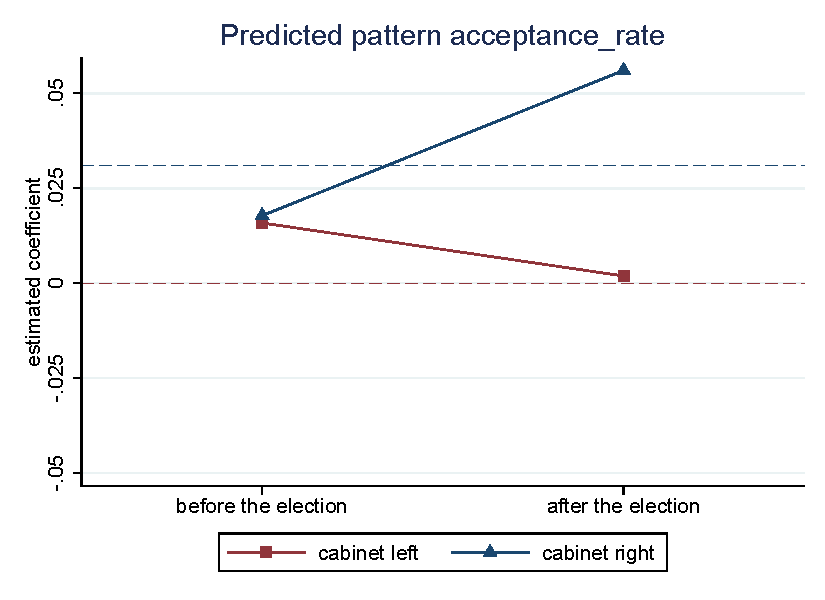
\includegraphics[width=1\textwidth]{figures_edited/acceptance_rate_graph1_baseline.pdf}
	\caption{Acceptance Rate: Predicted Pattern}
\end{figure}

\begin{table}[!ht]\centering
\renewcommand{\arraystretch}{1.25}
\def\sym#1{\ifmmode^{#1}\else\(^{#1}\)\fi}
\caption{Acceptance Rate: Predicted Pattern}
\begin{tabular}[]{l*{2}{c}}
	\hline\hline
	                    &\multicolumn{1}{c}{(1)}&\multicolumn{1}{c}{(2)}\\
                    &\multicolumn{1}{c}{left}&\multicolumn{1}{c}{right}\\
\hline
before              &     0.00122         &   -0.000995         \\
                    &   (0.00649)         &   (0.00651)         \\
after               &     -0.0107         &      0.0311\sym{***}\\
                    &   (0.00578)         &   (0.00716)         \\
\hline
Observations        &       18226         &       18226         \\

	\hline\hline
	\multicolumn{3}{c}{\footnotesize Standard errors in parentheses} \\
	\multicolumn{3}{c}{\footnotesize (\sym{*} \(p<0.05\), \sym{**} \(p<0.01\), \sym{***} \(p<0.001\))}\\
\end{tabular}
\end{table}

\clearpage
\textbf{Baseline Specification - Model 2}
\begin{table}[!ht]\centering
	\scriptsize
	\renewcommand{\arraystretch}{1.05}
	\def\sym#1{\ifmmode^{#1}\else\(^{#1}\)\fi}
	\caption{Determinants of acceptance rate}
	\begin{tabular}{l*{3}{c}}
		\hline\hline
		                    &\multicolumn{1}{c}{(1)}         &\multicolumn{1}{c}{(2)}         &\multicolumn{1}{c}{(3)}         \\
\hline
Political Terror Scale&      0.0196\sym{*}  &      0.0202\sym{*}  &                     \\
                    &   (0.00888)         &   (0.00934)         &                     \\
Civic Liberty (FHI) &      0.0354\sym{*}  &      0.0364\sym{*}  &                     \\
                    &    (0.0174)         &    (0.0167)         &                     \\
Political Rights (FHI)&    -0.00681         &    -0.00550         &                     \\
                    &    (0.0130)         &    (0.0136)         &                     \\
Quarterly civil war battle death (000s)&      0.0452\sym{***}&      0.0442\sym{***}&                     \\
                    &   (0.00439)         &   (0.00423)         &                     \\
Log origin country real GDP per capita&     -0.0355         &     -0.0285         &                     \\
                    &    (0.0203)         &    (0.0224)         &                     \\
Log destination country real GDP per capita&      -0.158         &      -0.157         &      -0.181         \\
                    &    (0.0895)         &    (0.0876)         &     (0.100)         \\
Quarterly unemployment rate at destination&    -0.00468\sym{**} &    -0.00509\sym{**} &    -0.00525\sym{**} \\
                    &   (0.00170)         &   (0.00164)         &   (0.00185)         \\
Log average past total asylum decisions per capita&     -0.0319\sym{***}&     -0.0391\sym{***}&     -0.0329\sym{***}\\
                    &   (0.00755)         &   (0.00745)         &   (0.00816)         \\
Log average past dyadic asylum decisions per capita&     0.00595         &      0.0130\sym{**} &     0.00402         \\
                    &   (0.00430)         &   (0.00409)         &   (0.00461)         \\
Cabinet position left * 6 quarters before the election&    -0.00677         &    -0.00531         &    -0.00591         \\
                    &    (0.0108)         &    (0.0104)         &    (0.0105)         \\
Cabinet position left * 5 quarters before the election&    -0.00215         &    0.000915         &    -0.00277         \\
                    &    (0.0104)         &    (0.0102)         &    (0.0107)         \\
Cabinet position left * 4 quarters before the election&     -0.0237         &     -0.0182         &     -0.0271         \\
                    &    (0.0134)         &    (0.0132)         &    (0.0136)         \\
Cabinet position left * 3 quarters before the election&    -0.00471         &    -0.00266         &    -0.00589         \\
                    &    (0.0132)         &    (0.0134)         &    (0.0123)         \\
Cabinet position left * 2 quarters before the election&      0.0145         &      0.0171         &      0.0177         \\
                    &   (0.00911)         &   (0.00952)         &   (0.00923)         \\
Cabinet position left * 1 quarters before the election&    0.000517         &     0.00427         &     0.00350         \\
                    &   (0.00903)         &   (0.00870)         &   (0.00927)         \\
Cabinet position left * election quarter&     0.00452         &     0.00778         &     0.00474         \\
                    &   (0.00961)         &   (0.00917)         &   (0.00962)         \\
Cabinet position left * 1 quarters after the election&     -0.0212\sym{**} &     -0.0168\sym{*}  &     -0.0198\sym{*}  \\
                    &   (0.00728)         &   (0.00729)         &   (0.00763)         \\
Cabinet position left * 2 quarters after the election&     -0.0183         &     -0.0180         &     -0.0145         \\
                    &   (0.00976)         &    (0.0102)         &   (0.00928)         \\
Cabinet position left * 3 quarters after the election&    -0.00615         &    -0.00617         &    -0.00541         \\
                    &   (0.00794)         &   (0.00777)         &   (0.00803)         \\
Cabinet position left * 4 quarters after the election&    -0.00409         &    -0.00634         &    -0.00202         \\
                    &    (0.0109)         &    (0.0111)         &    (0.0112)         \\
Cabinet position left * 5 quarters after the election&    -0.00502         &    -0.00758         &    -0.00432         \\
                    &    (0.0102)         &    (0.0102)         &    (0.0106)         \\
Cabinet position left * 6 quarters after the election&    -0.00722         &     -0.0105         &    -0.00898         \\
                    &   (0.00907)         &   (0.00849)         &   (0.00913)         \\
Cabinet position right * 6 quarters before the election&    -0.00487         &    -0.00198         &    -0.00754         \\
                    &   (0.00827)         &   (0.00846)         &   (0.00836)         \\
Cabinet position right * 5 quarters before the election&    0.000614         &     0.00516         &    0.000291         \\
                    &   (0.00783)         &   (0.00776)         &   (0.00846)         \\
Cabinet position right * 4 quarters before the election&    -0.00190         &     0.00244         &    -0.00204         \\
                    &    (0.0119)         &    (0.0116)         &    (0.0121)         \\
Cabinet position right * 3 quarters before the election&     -0.0175         &     -0.0170         &     -0.0167         \\
                    &   (0.00987)         &    (0.0104)         &   (0.00986)         \\
Cabinet position right * 2 quarters before the election&    -0.00848         &    -0.00578         &    -0.00776         \\
                    &    (0.0103)         &   (0.00979)         &    (0.0111)         \\
Cabinet position right * 1 quarters before the election&      0.0130         &      0.0120         &      0.0154         \\
                    &    (0.0110)         &    (0.0108)         &    (0.0119)         \\
Cabinet position right * election quarter&     0.00304         &     0.00478         &     0.00358         \\
                    &    (0.0129)         &    (0.0119)         &    (0.0134)         \\
Cabinet position right * 1 quarters after the election&      0.0237         &      0.0260\sym{*}  &      0.0209         \\
                    &    (0.0126)         &    (0.0119)         &    (0.0129)         \\
Cabinet position right * 2 quarters after the election&      0.0218         &      0.0242\sym{*}  &      0.0193         \\
                    &    (0.0111)         &    (0.0106)         &    (0.0107)         \\
Cabinet position right * 3 quarters after the election&      0.0372\sym{**} &      0.0348\sym{**} &      0.0344\sym{**} \\
                    &    (0.0127)         &    (0.0129)         &    (0.0128)         \\
Cabinet position right * 4 quarters after the election&      0.0206\sym{*}  &      0.0191\sym{*}  &      0.0208\sym{*}  \\
                    &   (0.00880)         &   (0.00849)         &   (0.00937)         \\
Cabinet position right * 5 quarters after the election&      0.0416\sym{**} &      0.0411\sym{**} &      0.0408\sym{**} \\
                    &    (0.0120)         &    (0.0118)         &    (0.0123)         \\
Cabinet position right * 6 quarters after the election&      0.0279\sym{**} &      0.0275\sym{**} &      0.0278\sym{***}\\
                    &   (0.00819)         &   (0.00783)         &   (0.00778)         \\
\hline
Observations        &       18029         &       18029         &       18029         \\
Adjusted \(R^{2}\)  &       0.154         &       0.101         &       0.099         \\
Fixed Effects       &           O         &       D x O         &       O x T         \\
Destination dummies &         Yes         &          No         &         Yes         \\
Quarter-Year dummies&         Yes         &         Yes         &          No         \\

		\hline\hline
		\multicolumn{4}{c}{\footnotesize Standard errors in parentheses (\sym{*} \(p<0.05\), \sym{**} \(p<0.01\), \sym{***} \(p<0.001\))}\\
	\end{tabular}
\end{table}


\clearpage
\textbf{Baseline Specification - Model 2}
\begin{figure}[!ht]
	\centering
	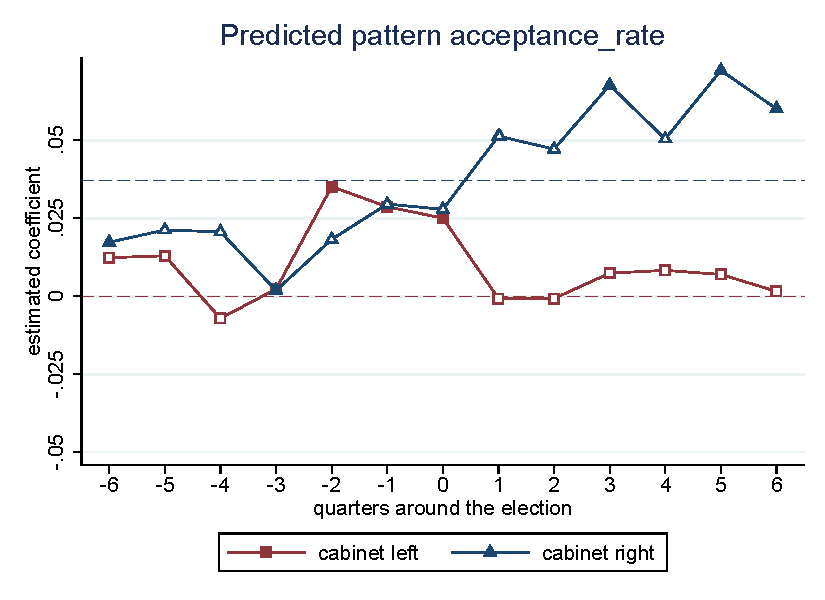
\includegraphics[width=0.7\textwidth]{figures_edited/acceptance_rate_graph2_baseline.pdf}
	\caption{Acceptance Rate: Predicted Pattern}
\end{figure}

\begin{table}[!ht]\centering
	\footnotesize
	\renewcommand{\arraystretch}{1.2}
	\def\sym#1{\ifmmode^{#1}\else\(^{#1}\)\fi}
	\caption{Acceptance Rate: Predicted Pattern}
	\begin{tabular}{l*{2}{c}}
		\hline\hline
		                    &\multicolumn{1}{c}{(1)}&\multicolumn{1}{c}{(2)}\\
                    &\multicolumn{1}{c}{left}&\multicolumn{1}{c}{right}\\
\hline
 6 quarters before the election&    -0.00325         &    -0.00427         \\
                    &    (0.0107)         &   (0.00853)         \\
 5 quarters before the election&   -0.000750         &     0.00378         \\
                    &    (0.0102)         &   (0.00780)         \\
 4 quarters before the election&     -0.0187         &     0.00214         \\
                    &    (0.0131)         &    (0.0117)         \\
 3 quarters before the election&    -0.00390         &     -0.0183         \\
                    &    (0.0133)         &    (0.0103)         \\
 2 quarters before the election&      0.0182         &    -0.00394         \\
                    &   (0.00978)         &   (0.00997)         \\
 1 quarters before the election&     0.00587         &      0.0116         \\
                    &   (0.00893)         &    (0.0107)         \\
Quarter of the election&     0.00826         &     0.00429         \\
                    &   (0.00927)         &    (0.0119)         \\
 1 quarters after the election&     -0.0170\sym{*}  &      0.0267\sym{*}  \\
                    &   (0.00724)         &    (0.0113)         \\
 2 quarters after the election&     -0.0195         &      0.0254\sym{*}  \\
                    &    (0.0105)         &    (0.0107)         \\
 3 quarters after the election&    -0.00554         &      0.0343\sym{**} \\
                    &   (0.00771)         &    (0.0128)         \\
 4 quarters after the election&    -0.00478         &      0.0179\sym{*}  \\
                    &    (0.0108)         &   (0.00839)         \\
 5 quarters after the election&    -0.00733         &      0.0407\sym{***}\\
                    &    (0.0102)         &    (0.0118)         \\
 6 quarters after the election&     -0.0103         &      0.0260\sym{***}\\
                    &   (0.00849)         &   (0.00778)         \\
\hline
Observations        &       18091         &       18091         \\

		\hline\hline
		\multicolumn{3}{c}{\footnotesize Standard errors in parentheses} \\
		\multicolumn{3}{c}{\footnotesize (\sym{*} \(p<0.05\), \sym{**} \(p<0.01\), \sym{***} \(p<0.001\))}\\
	\end{tabular}
\end{table}

% ===============================================================================================================


\FloatBarrier
\clearpage
\subsection{Robustness}

\subsubsection{Use destination, origin and time fixed effects}
\textbf{ R1: Use destination, origin and time fixed effects - Model 1}

\begin{figure}[!ht]
	\centering
	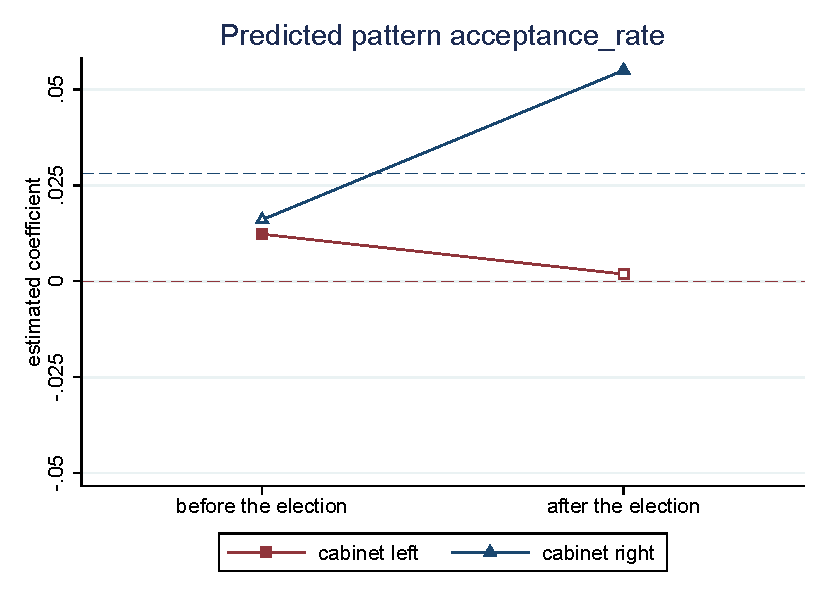
\includegraphics[width=1\textwidth]{figures_edited/acceptance_rate_graph1_R1.pdf}
	\caption{R1: Acceptance Rate: Predicted Pattern}
\end{figure}

\begin{table}[!ht]\centering
	\renewcommand{\arraystretch}{1.25}
	\def\sym#1{\ifmmode^{#1}\else\(^{#1}\)\fi}
	\caption{R1: Acceptance Rate: Predicted Pattern}
	\begin{tabular}{l*{2}{c}}
		\hline\hline
		                    &\multicolumn{1}{c}{(1)}&\multicolumn{1}{c}{(2)}\\
                    &\multicolumn{1}{c}{left}&\multicolumn{1}{c}{right}\\
\hline
before              &      0.0123\sym{*}  &     -0.0120         \\
                    &   (0.00607)         &   (0.00809)         \\
after               &     0.00188         &      0.0269\sym{***}\\
                    &   (0.00518)         &   (0.00562)         \\
\hline
Observations        &       17193         &       17193         \\

		\hline\hline
		\multicolumn{3}{c}{\footnotesize Standard errors in parentheses} \\
		\multicolumn{3}{c}{\footnotesize (\sym{*} \(p<0.05\), \sym{**} \(p<0.01\), \sym{***} \(p<0.001\))}\\
	\end{tabular}
\end{table}

\clearpage
\textbf{ R1: Use destination, origin and time fixed effects - Model 2}
\begin{figure}[!ht]
	\centering
	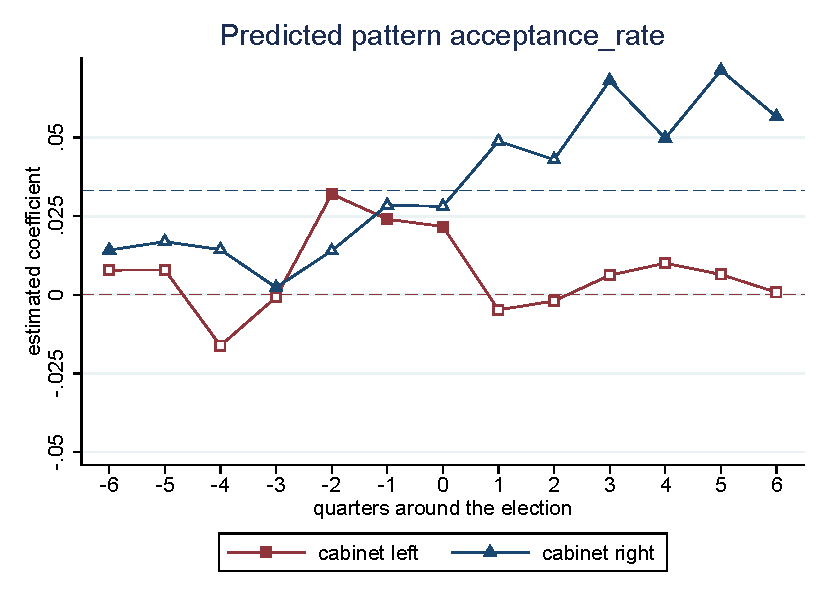
\includegraphics[width=0.7\textwidth]{figures_edited/acceptance_rate_graph2_R1.pdf}
	\caption{R1: Acceptance Rate: Predicted Pattern}
\end{figure}

\begin{table}[!ht]\centering
	\footnotesize
	\renewcommand{\arraystretch}{1.2}
	\def\sym#1{\ifmmode^{#1}\else\(^{#1}\)\fi}
	\caption{R1: Acceptance Rate: Predicted Pattern}
	\begin{tabular}{l*{2}{c}}
		\hline\hline
		                    &\multicolumn{1}{c}{(1)}&\multicolumn{1}{c}{(2)}\\
                    &\multicolumn{1}{c}{left}&\multicolumn{1}{c}{right}\\
\hline
 6 quarters before the election&     0.00785         &     -0.0188\sym{*}  \\
                    &    (0.0103)         &   (0.00794)         \\
 5 quarters before the election&     0.00788         &     -0.0161         \\
                    &    (0.0109)         &   (0.00972)         \\
 4 quarters before the election&     -0.0162         &     -0.0187         \\
                    &   (0.00966)         &    (0.0115)         \\
 3 quarters before the election&   -0.000749         &     -0.0307\sym{**} \\
                    &    (0.0130)         &    (0.0114)         \\
 2 quarters before the election&      0.0320\sym{***}&     -0.0190         \\
                    &   (0.00861)         &    (0.0115)         \\
 1 quarters before the election&      0.0240\sym{*}  &    -0.00457         \\
                    &   (0.00945)         &    (0.0115)         \\
Quarter of the election&      0.0217\sym{*}  &    -0.00489         \\
                    &   (0.00945)         &    (0.0147)         \\
 1 quarters after the election&    -0.00478         &      0.0158         \\
                    &   (0.00787)         &    (0.0126)         \\
 2 quarters after the election&    -0.00195         &     0.00992         \\
                    &   (0.00770)         &   (0.00896)         \\
 3 quarters after the election&     0.00622         &      0.0351\sym{***}\\
                    &   (0.00780)         &    (0.0105)         \\
 4 quarters after the election&      0.0101         &      0.0167\sym{*}  \\
                    &   (0.00792)         &   (0.00818)         \\
 5 quarters after the election&     0.00646         &      0.0383\sym{***}\\
                    &   (0.00827)         &    (0.0106)         \\
 6 quarters after the election&    0.000793         &      0.0236\sym{**} \\
                    &    (0.0105)         &   (0.00753)         \\
\hline
Observations        &       17193         &       17193         \\

		\hline\hline
		\multicolumn{3}{c}{\footnotesize Standard errors in parentheses} \\
		\multicolumn{3}{c}{\footnotesize (\sym{*} \(p<0.05\), \sym{**} \(p<0.01\), \sym{***} \(p<0.001\))}\\
	\end{tabular}
\end{table}

% ===============================================================================================================

\FloatBarrier
\clearpage
\subsubsection{Use destination and origin*time fixed effects}
\textbf{R2: Use destination and origin*time fixed effects - Model 1}

\begin{figure}[!ht]
	\centering
	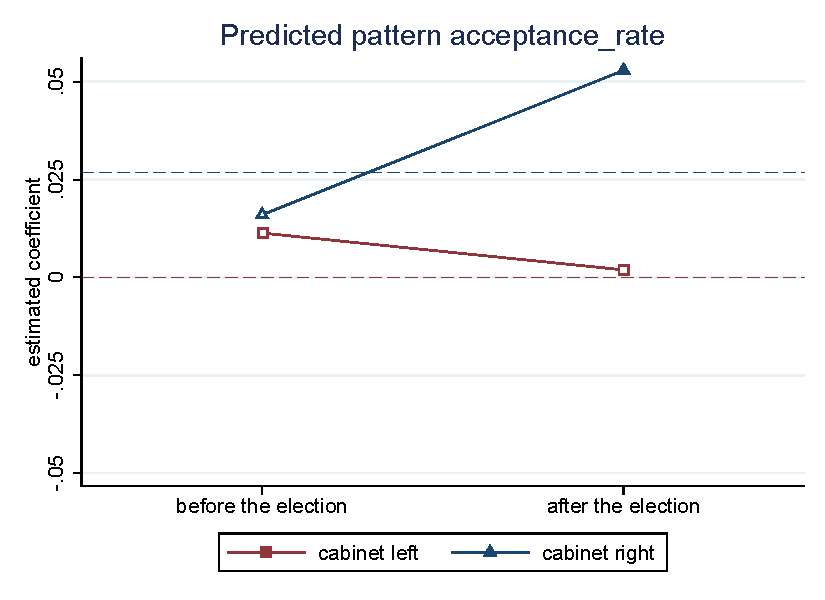
\includegraphics[width=1\textwidth]{figures_edited/acceptance_rate_graph1_R2.pdf}
	\caption{R2: Acceptance Rate: Predicted Pattern}
\end{figure}

\begin{table}[!ht]\centering
	\renewcommand{\arraystretch}{1.25}
	\def\sym#1{\ifmmode^{#1}\else\(^{#1}\)\fi}
	\caption{R2: Acceptance Rate: Predicted Pattern}
	\begin{tabular}{l*{2}{c}}
		\hline\hline
		                    &\multicolumn{1}{c}{(1)}&\multicolumn{1}{c}{(2)}\\
                    &\multicolumn{1}{c}{left}&\multicolumn{1}{c}{right}\\
\hline
before              &      0.0113         &     -0.0107         \\
                    &   (0.00622)         &   (0.00823)         \\
after               &     0.00192         &      0.0262\sym{***}\\
                    &   (0.00555)         &   (0.00583)         \\
\hline
Observations        &       17193         &       17193         \\

		\hline\hline
		\multicolumn{3}{c}{\footnotesize Standard errors in parentheses} \\
		\multicolumn{3}{c}{\footnotesize (\sym{*} \(p<0.05\), \sym{**} \(p<0.01\), \sym{***} \(p<0.001\))}\\
	\end{tabular}
\end{table}

\clearpage
\textbf{R2: Use destination and origin*time fixed effects - Model 2}
\begin{figure}[!ht]
	\centering
	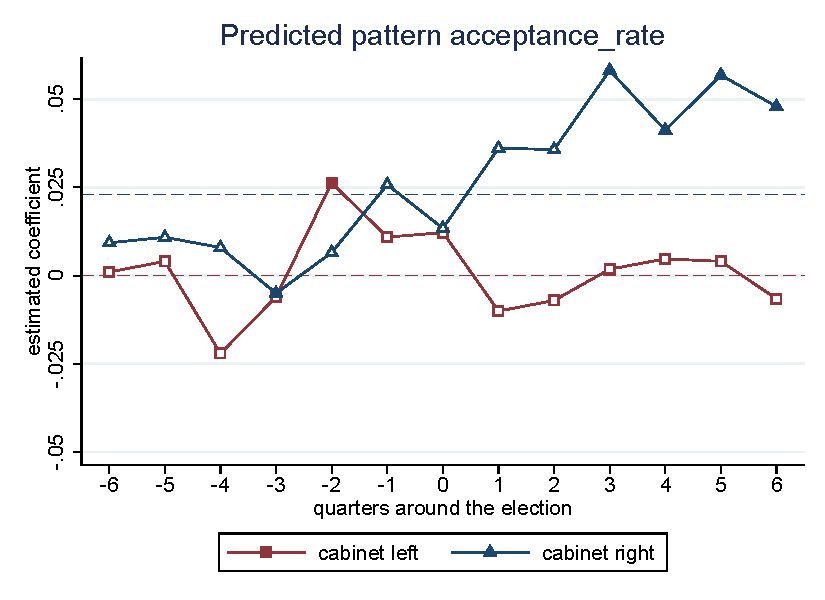
\includegraphics[width=0.7\textwidth]{figures_edited/acceptance_rate_graph2_R2.pdf}
	\caption{R2: Acceptance Rate: Predicted Pattern}
\end{figure}

\begin{table}[!ht]\centering
	\footnotesize
	\renewcommand{\arraystretch}{1.2}
	\def\sym#1{\ifmmode^{#1}\else\(^{#1}\)\fi}
	\caption{R2: Acceptance Rate: Predicted Pattern}
	\begin{tabular}{l*{2}{c}}
		\hline\hline
		                    &\multicolumn{1}{c}{(1)}&\multicolumn{1}{c}{(2)}\\
                    &\multicolumn{1}{c}{left}&\multicolumn{1}{c}{right}\\
\hline
 6 quarters before the election&     0.00743         &     -0.0193\sym{*}  \\
                    &    (0.0110)         &   (0.00830)         \\
 5 quarters before the election&     0.00721         &     -0.0150         \\
                    &    (0.0117)         &    (0.0104)         \\
 4 quarters before the election&     -0.0207\sym{*}  &     -0.0170         \\
                    &    (0.0102)         &    (0.0113)         \\
 3 quarters before the election&    -0.00326         &     -0.0288\sym{*}  \\
                    &    (0.0124)         &    (0.0119)         \\
 2 quarters before the election&      0.0330\sym{***}&     -0.0198         \\
                    &   (0.00924)         &    (0.0116)         \\
 1 quarters before the election&      0.0246\sym{**} &   -0.000716         \\
                    &   (0.00950)         &    (0.0115)         \\
Quarter of the election&      0.0210\sym{*}  &    -0.00526         \\
                    &   (0.00949)         &    (0.0150)         \\
 1 quarters after the election&    -0.00480         &      0.0151         \\
                    &   (0.00848)         &    (0.0132)         \\
 2 quarters after the election&    0.000366         &     0.00834         \\
                    &   (0.00749)         &   (0.00882)         \\
 3 quarters after the election&     0.00455         &      0.0339\sym{**} \\
                    &   (0.00849)         &    (0.0107)         \\
 4 quarters after the election&      0.0112         &      0.0158         \\
                    &   (0.00837)         &   (0.00865)         \\
 5 quarters after the election&     0.00695         &      0.0368\sym{***}\\
                    &   (0.00903)         &    (0.0107)         \\
 6 quarters after the election&    -0.00174         &      0.0245\sym{***}\\
                    &    (0.0111)         &   (0.00734)         \\
\hline
Observations        &       17193         &       17193         \\

		\hline\hline
		\multicolumn{3}{c}{\footnotesize Standard errors in parentheses} \\
		\multicolumn{3}{c}{\footnotesize (\sym{*} \(p<0.05\), \sym{**} \(p<0.01\), \sym{***} \(p<0.001\))}\\
	\end{tabular}
\end{table}


% ===============================================================================================================


\clearpage
\FloatBarrier
\subsubsection{Control for past asylum applications}
\begin{table}[!ht]\centering
	\renewcommand{\arraystretch}{1.25}
	\small
	\def\sym#1{\ifmmode^{#1}\else\(^{#1}\)\fi}
	\caption{R3: Determinants of acceptance rate}
	\begin{tabular}{l*{3}{c}}
		\hline\hline
		                                        &\multicolumn{1}{c}{(1)}         &\multicolumn{1}{c}{(2)}         &\multicolumn{1}{c}{(3)}         \\
\hline
Political Terror Scale                  &    0.0168         &    0.0216\sym{*}  &                   \\
                                        & (0.00989)         &  (0.0103)         &                   \\
Civic Liberty (FHI)                     &    0.0407\sym{*}  &    0.0378         &                   \\
                                        &  (0.0190)         &  (0.0192)         &                   \\
Political Rights (FHI)                  &  -0.00987         &  -0.00840         &                   \\
                                        &  (0.0150)         &  (0.0160)         &                   \\
Quarterly civil war battle death (000s) &    0.0452\sym{***}&    0.0451\sym{***}&                   \\
                                        & (0.00430)         & (0.00480)         &                   \\
Log origin country real GDP per capita  &   -0.0149         &   -0.0173         &                   \\
                                        &  (0.0317)         &  (0.0365)         &                   \\
Log migrant stock in 2000/1             & -0.000776         &                   & -0.000274         \\
                                        & (0.00241)         &                   & (0.00246)         \\
Log distance from origin to destination &    0.0141         &                   &    0.0154         \\
                                        &  (0.0234)         &                   &  (0.0238)         \\
Log destination country real GDP per capita&    0.0684         &    0.0898         &    0.0717         \\
                                        &  (0.0697)         &  (0.0733)         &  (0.0658)         \\
Quarterly unemployment rate at destination&  -0.00109         &  -0.00119         &  -0.00135         \\
                                        & (0.00122)         & (0.00112)         & (0.00124)         \\
Log average past total asylum decisions per capita&    -152.9\sym{***}&    -158.5\sym{***}&    -150.8\sym{***}\\
                                        &   (36.22)         &   (36.69)         &   (37.57)         \\
Log average past dyadic asylum decisions per capita&     416.3\sym{*}  &     300.1         &     274.0         \\
                                        &   (196.9)         &   (228.7)         &   (209.7)         \\
Log average past asylum applications at destination per capita&  -0.00442         &  -0.00601         &  -0.00514         \\
                                        & (0.00807)         & (0.00803)         & (0.00830)         \\
Weighted cabinet position right         &    0.0283\sym{*}  &    0.0308\sym{**} &    0.0271\sym{*}  \\
                                        &  (0.0108)         &  (0.0111)         &  (0.0112)         \\
Cabinet position left * Before the election&    0.0127\sym{*}  &    0.0157\sym{*}  &    0.0116         \\
                                        & (0.00596)         & (0.00594)         & (0.00608)         \\
Cabinet position left * After the election&   0.00252         &   0.00259         &   0.00253         \\
                                        & (0.00522)         & (0.00547)         & (0.00566)         \\
Cabinet position right * Before the election&   -0.0127         &   -0.0132         &   -0.0113         \\
                                        & (0.00785)         & (0.00767)         & (0.00795)         \\
Cabinet position right * After the election&    0.0269\sym{***}&    0.0252\sym{***}&    0.0261\sym{***}\\
                                        & (0.00573)         & (0.00545)         & (0.00595)         \\
\hline
Observations                            &     17138         &     17138         &     17138         \\
Adjusted \(R^{2}\)                      &     0.156         &     0.106         &     0.104         \\
Fixed Effects                           &         O         &     D x O         &     O x T         \\
Destination dummies                     &       Yes         &        No         &       Yes         \\
Quarter-Year dummies                    &       Yes         &       Yes         &        No         \\

		\hline\hline
		\multicolumn{4}{l}{\footnotesize Standard errors in parentheses (\sym{*} \(p<0.05\), \sym{**} \(p<0.01\), \sym{***} \(p<0.001\))}\\
	\end{tabular}
\end{table}

\clearpage
\textbf{R3: Control for past asylum applications - Model 1}
\begin{figure}[!ht]
	\centering
	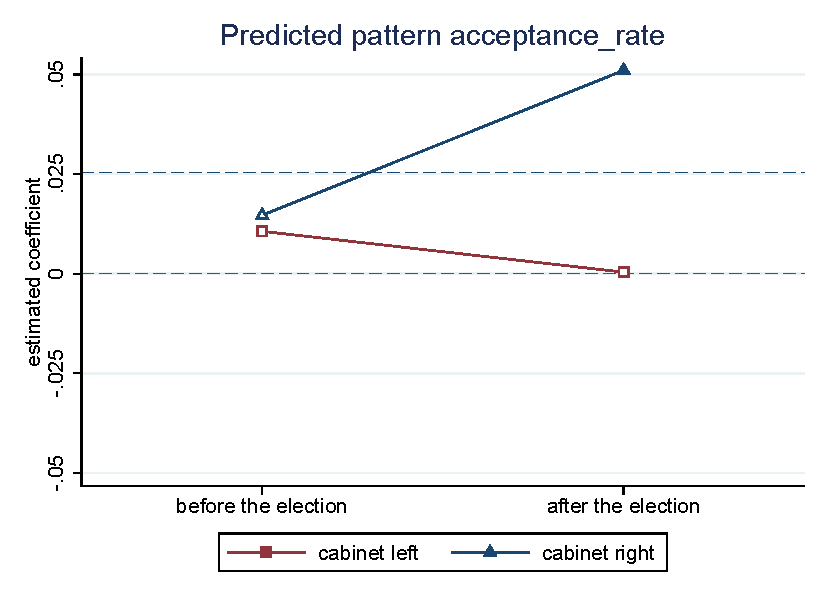
\includegraphics[width=1\textwidth]{figures_edited/acceptance_rate_graph1_R3.pdf}
	\caption{R3: Acceptance Rate: Predicted Pattern}
\end{figure}

\begin{table}[!ht]\centering
	\renewcommand{\arraystretch}{1.25}
	\def\sym#1{\ifmmode^{#1}\else\(^{#1}\)\fi}
	\caption{R3: Acceptance Rate: Predicted Pattern}
	\begin{tabular}{l*{2}{c}}
		\hline\hline
		                    &\multicolumn{1}{c}{(1)}&\multicolumn{1}{c}{(2)}\\
                    &\multicolumn{1}{c}{left}&\multicolumn{1}{c}{right}\\
\hline
before              &      0.0157\sym{**} &     -0.0132         \\
                    &   (0.00594)         &   (0.00767)         \\
after               &     0.00259         &      0.0252\sym{***}\\
                    &   (0.00547)         &   (0.00545)         \\
\hline
Observations        &       17138         &       17138         \\

		\hline\hline
		\multicolumn{3}{c}{\footnotesize Standard errors in parentheses} \\
	    \multicolumn{3}{c}{\footnotesize (\sym{*} \(p<0.05\), \sym{**} \(p<0.01\), \sym{***} \(p<0.001\))}\\
	\end{tabular}
\end{table}

\clearpage
\textbf{R3: Control for past asylum applications - Model 2}
\begin{figure}[!ht]
	\centering
	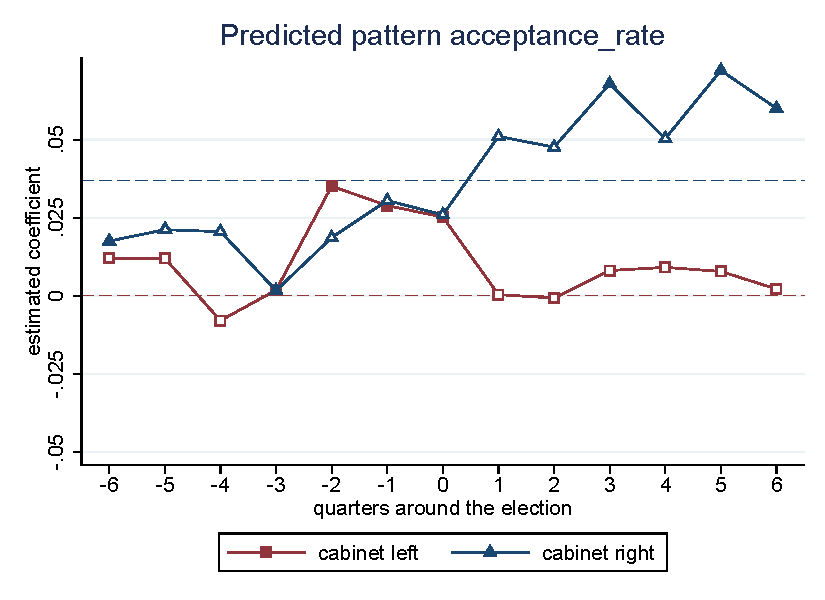
\includegraphics[width=0.7\textwidth]{figures_edited/acceptance_rate_graph2_R3.pdf}
	\caption{R3: Acceptance Rate: Predicted Pattern}
\end{figure}

\begin{table}[!ht]\centering
	\footnotesize
	\renewcommand{\arraystretch}{1.2}
	\def\sym#1{\ifmmode^{#1}\else\(^{#1}\)\fi}
	\caption{R3: Acceptance Rate: Predicted Pattern}
	\begin{tabular}{l*{2}{c}}
		\hline\hline
		                    &\multicolumn{1}{c}{(1)}&\multicolumn{1}{c}{(2)}\\
                    &\multicolumn{1}{c}{left}&\multicolumn{1}{c}{right}\\
\hline
 6 quarters before the election&      0.0121         &     -0.0193\sym{*}  \\
                    &   (0.00995)         &   (0.00755)         \\
 5 quarters before the election&      0.0121         &     -0.0156         \\
                    &    (0.0101)         &   (0.00938)         \\
 4 quarters before the election&    -0.00788         &     -0.0162         \\
                    &   (0.00915)         &    (0.0107)         \\
 3 quarters before the election&     0.00188         &     -0.0351\sym{**} \\
                    &    (0.0133)         &    (0.0117)         \\
 2 quarters before the election&      0.0352\sym{***}&     -0.0181         \\
                    &   (0.00904)         &    (0.0108)         \\
 1 quarters before the election&      0.0290\sym{**} &    -0.00627         \\
                    &   (0.00940)         &    (0.0109)         \\
Quarter of the election&      0.0253\sym{**} &     -0.0108         \\
                    &   (0.00904)         &    (0.0134)         \\
 1 quarters after the election&    0.000442         &      0.0143         \\
                    &   (0.00837)         &    (0.0122)         \\
 2 quarters after the election&   -0.000675         &      0.0108         \\
                    &   (0.00883)         &   (0.00918)         \\
 3 quarters after the election&     0.00815         &      0.0311\sym{**} \\
                    &   (0.00803)         &    (0.0107)         \\
 4 quarters after the election&     0.00917         &      0.0136         \\
                    &   (0.00814)         &   (0.00768)         \\
 5 quarters after the election&     0.00787         &      0.0354\sym{***}\\
                    &   (0.00819)         &    (0.0106)         \\
 6 quarters after the election&     0.00222         &      0.0232\sym{**} \\
                    &    (0.0105)         &   (0.00719)         \\
\hline
Observations        &       17138         &       17138         \\

		\hline\hline
		\multicolumn{3}{c}{\footnotesize Standard errors in parentheses} \\
		\multicolumn{3}{c}{\footnotesize (\sym{*} \(p<0.05\), \sym{**} \(p<0.01\), \sym{***} \(p<0.001\))} \\
	\end{tabular}
\end{table}


% ===============================================================================================================


\clearpage
\FloatBarrier
\subsubsection{Do not include cabinet right dummy}
\begin{table}[!ht]\centering
	\renewcommand{\arraystretch}{1.25}
	\small
	\def\sym#1{\ifmmode^{#1}\else\(^{#1}\)\fi}
	\caption{R4: Determinants of acceptance rate}
	\begin{tabular}{l*{3}{c}}
		\hline\hline
		                                        &\multicolumn{1}{c}{(1)}         &\multicolumn{1}{c}{(2)}         &\multicolumn{1}{c}{(3)}         \\
\hline
Political Terror Scale                  &    0.0167         &    0.0218\sym{*}  &                   \\
                                        & (0.00983)         &  (0.0102)         &                   \\
Civic Liberty (FHI)                     &    0.0405\sym{*}  &    0.0375         &                   \\
                                        &  (0.0191)         &  (0.0192)         &                   \\
Political Rights (FHI)                  &  -0.00985         &  -0.00810         &                   \\
                                        &  (0.0150)         &  (0.0162)         &                   \\
Quarterly civil war battle death (000s) &    0.0451\sym{***}&    0.0451\sym{***}&                   \\
                                        & (0.00430)         & (0.00475)         &                   \\
Log origin country real GDP per capita  &   -0.0162         &   -0.0197         &                   \\
                                        &  (0.0315)         &  (0.0365)         &                   \\
Log migrant stock in 2000/1             & -0.000682         &                   & -0.000188         \\
                                        & (0.00240)         &                   & (0.00245)         \\
Log distance from origin to destination &    0.0143         &                   &    0.0154         \\
                                        &  (0.0233)         &                   &  (0.0235)         \\
Log destination country real GDP per capita&    0.0676         &    0.0981         &    0.0722         \\
                                        &  (0.0683)         &  (0.0724)         &  (0.0658)         \\
Quarterly unemployment rate at destination&  -0.00136         &  -0.00135         &  -0.00159         \\
                                        & (0.00128)         & (0.00118)         & (0.00131)         \\
Log average past total asylum decisions per capita&    -161.4\sym{***}&    -170.0\sym{***}&    -160.0\sym{***}\\
                                        &   (36.36)         &   (37.52)         &   (37.99)         \\
Log average past dyadic asylum decisions per capita&     419.7\sym{*}  &     296.5         &     272.8         \\
                                        &   (195.3)         &   (232.4)         &   (208.1)         \\
Cabinet position left * Before the election&  -0.00236         & -0.000253         &  -0.00256         \\
                                        & (0.00680)         & (0.00677)         & (0.00708)         \\
Cabinet position left * After the election&   -0.0122         &   -0.0135\sym{*}  &   -0.0115         \\
                                        & (0.00608)         & (0.00625)         & (0.00615)         \\
Cabinet position right * Before the election&   0.00104         &   0.00108         &   0.00168         \\
                                        & (0.00690)         & (0.00648)         & (0.00722)         \\
Cabinet position right * After the election&    0.0407\sym{***}&    0.0399\sym{***}&    0.0392\sym{***}\\
                                        & (0.00758)         & (0.00713)         & (0.00741)         \\
\hline
Observations                            &     17193         &     17193         &     17193         \\
Adjusted \(R^{2}\)                      &     0.155         &     0.104         &     0.103         \\
Fixed Effects                           &         O         &     D x O         &     O x T         \\
Destination dummies                     &       Yes         &        No         &       Yes         \\
Quarter-Year dummies                    &       Yes         &       Yes         &        No         \\

		\hline\hline
		\multicolumn{4}{l}{\footnotesize Standard errors in parentheses (\sym{*} \(p<0.05\), \sym{**} \(p<0.01\), \sym{***} \(p<0.001\))}\\
	\end{tabular}
\end{table}

\clearpage
\textbf{R4: Do not include cabinet right dummy - Model 1}
\begin{figure}[!ht]
	\centering
	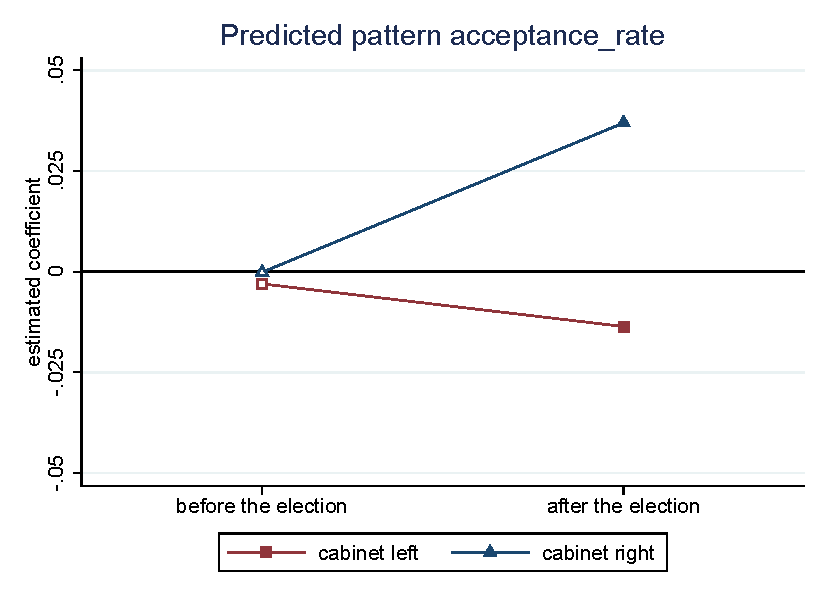
\includegraphics[width=1\textwidth]{figures_edited/acceptance_rate_graph1_R4.pdf}
	\caption{R4: Acceptance Rate: Predicted Pattern}
\end{figure}

\begin{table}[!ht]\centering
	\renewcommand{\arraystretch}{1.25}
	\def\sym#1{\ifmmode^{#1}\else\(^{#1}\)\fi}
	\caption{R4: Acceptance Rate: Predicted Pattern}
	\begin{tabular}{l*{2}{c}}
		\hline\hline
		                    &\multicolumn{1}{c}{(1)}&\multicolumn{1}{c}{(2)}\\
                    &\multicolumn{1}{c}{left}&\multicolumn{1}{c}{right}\\
\hline
before              &   -0.000253         &     0.00108         \\
                    &   (0.00677)         &   (0.00648)         \\
after               &     -0.0135\sym{*}  &      0.0399\sym{***}\\
                    &   (0.00625)         &   (0.00713)         \\
\hline
Observations        &       17193         &       17193         \\

		\hline\hline
		\multicolumn{3}{c}{\footnotesize Standard errors in parentheses} \\
		\multicolumn{3}{c}{\footnotesize (\sym{*} \(p<0.05\), \sym{**} \(p<0.01\), \sym{***} \(p<0.001\))}\\
	\end{tabular}
\end{table}

\clearpage
\textbf{R4: Do not include cabinet right dummy - Model 2}
\begin{figure}[!ht]
	\centering
	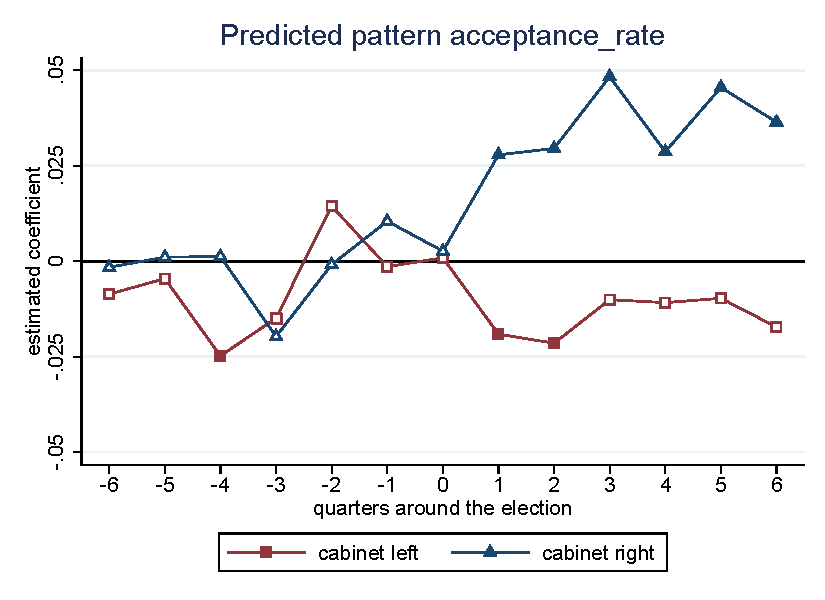
\includegraphics[width=0.7\textwidth]{figures_edited/acceptance_rate_graph2_R4.pdf}
	\caption{R4: Acceptance Rate: Predicted Pattern}
\end{figure}

\begin{table}[!ht]\centering
	\footnotesize
	\renewcommand{\arraystretch}{1.2}
	\def\sym#1{\ifmmode^{#1}\else\(^{#1}\)\fi}
	\caption{R4: Acceptance Rate: Predicted Pattern}
	\begin{tabular}{l*{2}{c}}
		\hline\hline
		                    &\multicolumn{1}{c}{(1)}&\multicolumn{1}{c}{(2)}\\
                    &\multicolumn{1}{c}{left}&\multicolumn{1}{c}{right}\\
\hline
 6 quarters before the election&    -0.00731         &    -0.00287         \\
                    &   (0.00959)         &   (0.00916)         \\
 5 quarters before the election&    -0.00645         &     0.00107         \\
                    &    (0.0105)         &   (0.00917)         \\
 4 quarters before the election&     -0.0262\sym{*}  &    0.000873         \\
                    &    (0.0113)         &    (0.0106)         \\
 3 quarters before the election&     -0.0164         &     -0.0179         \\
                    &    (0.0133)         &   (0.00935)         \\
 2 quarters before the election&      0.0166         &    -0.00106         \\
                    &   (0.00994)         &    (0.0109)         \\
 1 quarters before the election&     0.00869         &      0.0101         \\
                    &   (0.00883)         &    (0.0102)         \\
Quarter of the election&     0.00549         &     0.00843         \\
                    &   (0.00849)         &    (0.0115)         \\
 1 quarters after the election&     -0.0196\sym{*}  &      0.0320\sym{*}  \\
                    &   (0.00810)         &    (0.0127)         \\
 2 quarters after the election&     -0.0187\sym{*}  &      0.0281\sym{**} \\
                    &   (0.00852)         &    (0.0103)         \\
 3 quarters after the election&     -0.0106         &      0.0491\sym{***}\\
                    &   (0.00728)         &    (0.0119)         \\
 4 quarters after the election&     -0.0101         &      0.0316\sym{***}\\
                    &   (0.00969)         &   (0.00739)         \\
 5 quarters after the election&     -0.0115         &      0.0533\sym{***}\\
                    &   (0.00919)         &    (0.0122)         \\
 6 quarters after the election&     -0.0179         &      0.0399\sym{***}\\
                    &    (0.0107)         &   (0.00894)         \\
\hline
Observations        &       17193         &       17193         \\

		\hline\hline
		\multicolumn{3}{c}{\footnotesize Standard errors in parentheses} \\
		\multicolumn{3}{c}{\footnotesize (\sym{*} \(p<0.05\), \sym{**} \(p<0.01\), \sym{***} \(p<0.001\))} \\
	\end{tabular}
\end{table}


% ===============================================================================================================



\clearpage
\FloatBarrier
\subsubsection{Do not use lags for origin country variables}
\begin{table}[!ht]\centering
	\renewcommand{\arraystretch}{1.25}
	\small
	\def\sym#1{\ifmmode^{#1}\else\(^{#1}\)\fi}
	\caption{R5: Determinants of acceptance rate}
	\begin{tabular}{l*{3}{c}}
		\hline\hline
		                                        &\multicolumn{1}{c}{(1)}         &\multicolumn{1}{c}{(2)}         &\multicolumn{1}{c}{(3)}         \\
\hline
Political Terror Scale                  &    0.0142         &    0.0186\sym{*}  &                   \\
                                        & (0.00787)         & (0.00821)         &                   \\
Civic Liberty (FHI)                     &    0.0362\sym{*}  &    0.0352         &                   \\
                                        &  (0.0179)         &  (0.0181)         &                   \\
Political Rights (FHI)                  &  -0.00874         &  -0.00785         &                   \\
                                        &  (0.0131)         &  (0.0142)         &                   \\
Quarterly civil war battle death (000s) &    0.0374\sym{***}&    0.0369\sym{***}&                   \\
                                        & (0.00575)         & (0.00588)         &                   \\
Log origin country real GDP per capita  &   -0.0256         &   -0.0293         &                   \\
                                        &  (0.0334)         &  (0.0386)         &                   \\
Log migrant stock in 2000/1             & -0.000934         &                   & -0.000254         \\
                                        & (0.00241)         &                   & (0.00245)         \\
Log distance from origin to destination &    0.0140         &                   &    0.0153         \\
                                        &  (0.0232)         &                   &  (0.0234)         \\
Log destination country real GDP per capita&    0.0664         &    0.0944         &    0.0691         \\
                                        &  (0.0690)         &  (0.0730)         &  (0.0661)         \\
Quarterly unemployment rate at destination&  -0.00117         &  -0.00117         &  -0.00144         \\
                                        & (0.00125)         & (0.00115)         & (0.00130)         \\
Log average past total asylum decisions per capita&    -164.6\sym{***}&    -175.4\sym{***}&    -159.0\sym{***}\\
                                        &   (37.11)         &   (38.14)         &   (37.83)         \\
Log average past dyadic asylum decisions per capita&     528.4\sym{*}  &     491.1         &     272.5         \\
                                        &   (227.4)         &   (246.2)         &   (209.0)         \\
Weighted cabinet position right         &    0.0284\sym{*}  &    0.0311\sym{**} &    0.0269\sym{*}  \\
                                        &  (0.0108)         &  (0.0111)         &  (0.0112)         \\
Cabinet position left * Before the election&    0.0127\sym{*}  &    0.0161\sym{*}  &    0.0115         \\
                                        & (0.00612)         & (0.00611)         & (0.00625)         \\
Cabinet position left * After the election&   0.00192         &   0.00189         &   0.00196         \\
                                        & (0.00520)         & (0.00548)         & (0.00556)         \\
Cabinet position right * Before the election&   -0.0119         &   -0.0129         &   -0.0108         \\
                                        & (0.00820)         & (0.00804)         & (0.00821)         \\
Cabinet position right * After the election&    0.0272\sym{***}&    0.0253\sym{***}&    0.0262\sym{***}\\
                                        & (0.00567)         & (0.00540)         & (0.00589)         \\
\hline
Observations                            &     17193         &     17193         &     17193         \\
Adjusted \(R^{2}\)                      &     0.152         &     0.100         &     0.104         \\
Fixed Effects                           &         O         &     D x O         &     O x T         \\
Destination dummies                     &       Yes         &        No         &       Yes         \\
Quarter-Year dummies                    &       Yes         &       Yes         &        No         \\

		\hline\hline
		\multicolumn{4}{l}{\footnotesize Standard errors in parentheses (\sym{*} \(p<0.05\), \sym{**} \(p<0.01\), \sym{***} \(p<0.001\))}\\
	\end{tabular}
\end{table}

\clearpage
\textbf{R5: Do not use lags for origin country variables - Model 1}
\begin{figure}[!ht]
	\centering
	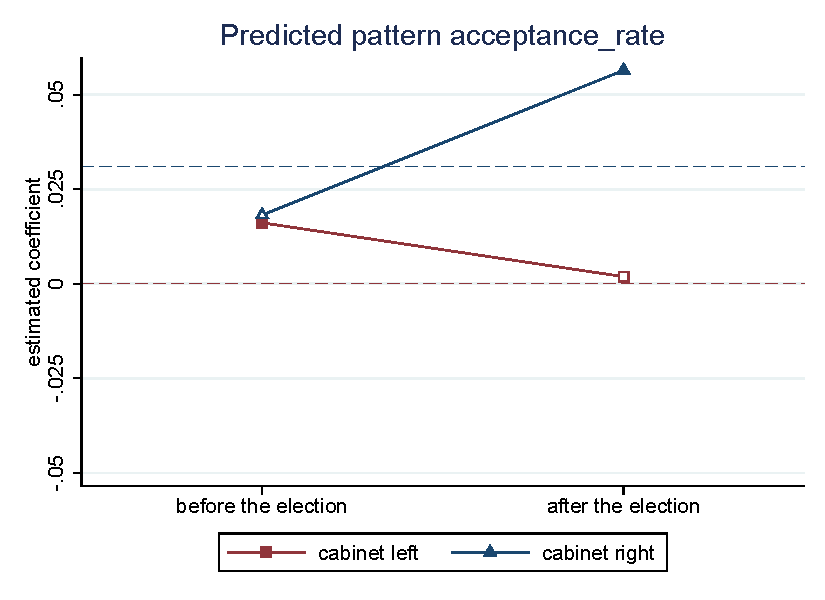
\includegraphics[width=1\textwidth]{figures_edited/acceptance_rate_graph1_R5.pdf}
	\caption{R5: Acceptance Rate: Predicted Pattern}
\end{figure}

\begin{table}[!ht]\centering
	\renewcommand{\arraystretch}{1.25}
	\def\sym#1{\ifmmode^{#1}\else\(^{#1}\)\fi}
	\caption{R5: Acceptance Rate: Predicted Pattern}
	\begin{tabular}{l*{2}{c}}
		\hline\hline
		                    &\multicolumn{1}{c}{(1)}&\multicolumn{1}{c}{(2)}\\
                    &\multicolumn{1}{c}{left}&\multicolumn{1}{c}{right}\\
\hline
before              &      0.0161\sym{**} &     -0.0129         \\
                    &   (0.00611)         &   (0.00804)         \\
after               &     0.00189         &      0.0253\sym{***}\\
                    &   (0.00548)         &   (0.00540)         \\
\hline
Observations        &       17193         &       17193         \\

		\hline\hline
		\multicolumn{3}{c}{\footnotesize Standard errors in parentheses} \\
		\multicolumn{3}{c}{\footnotesize (\sym{*} \(p<0.05\), \sym{**} \(p<0.01\), \sym{***} \(p<0.001\))}\\
	\end{tabular}
\end{table}

\clearpage
\textbf{R5: Do not use lags for origin country variables - Model 2}
\begin{figure}[!ht]
	\centering
	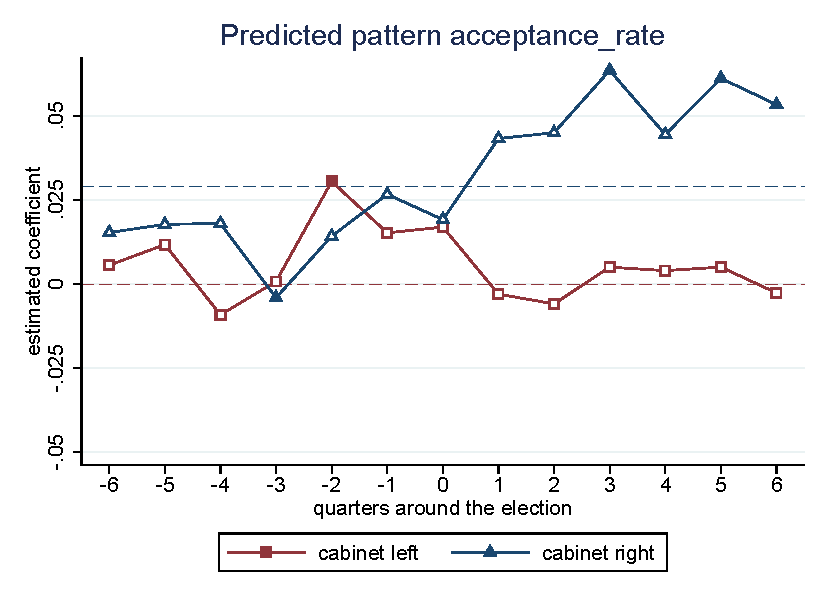
\includegraphics[width=0.7\textwidth]{figures_edited/acceptance_rate_graph2_R5.pdf}
	\caption{R5: Acceptance Rate: Predicted Pattern}
\end{figure}

\begin{table}[!ht]\centering
	\footnotesize
	\renewcommand{\arraystretch}{1.2}
	\def\sym#1{\ifmmode^{#1}\else\(^{#1}\)\fi}
	\caption{R5: Acceptance Rate: Predicted Pattern}
	\begin{tabular}{l*{2}{c}}
		\hline\hline
		                    &\multicolumn{1}{c}{(1)}&\multicolumn{1}{c}{(2)}\\
                    &\multicolumn{1}{c}{left}&\multicolumn{1}{c}{right}\\
\hline
 6 quarters before the election&      0.0121         &     -0.0196\sym{**} \\
                    &   (0.00998)         &   (0.00753)         \\
 5 quarters before the election&      0.0134         &     -0.0157         \\
                    &    (0.0104)         &   (0.00957)         \\
 4 quarters before the election&    -0.00638         &     -0.0154         \\
                    &   (0.00912)         &    (0.0109)         \\
 3 quarters before the election&     0.00264         &     -0.0349\sym{**} \\
                    &    (0.0133)         &    (0.0119)         \\
 2 quarters before the election&      0.0355\sym{***}&     -0.0193         \\
                    &   (0.00910)         &    (0.0111)         \\
 1 quarters before the election&      0.0284\sym{**} &    -0.00732         \\
                    &   (0.00974)         &    (0.0112)         \\
Quarter of the election&      0.0250\sym{**} &    -0.00874         \\
                    &   (0.00916)         &    (0.0144)         \\
 1 quarters after the election&   -0.000423         &      0.0142         \\
                    &   (0.00837)         &    (0.0123)         \\
 2 quarters after the election&   -0.000479         &      0.0102         \\
                    &   (0.00845)         &   (0.00917)         \\
 3 quarters after the election&     0.00733         &      0.0310\sym{**} \\
                    &   (0.00799)         &    (0.0105)         \\
 4 quarters after the election&     0.00833         &      0.0138         \\
                    &   (0.00811)         &   (0.00790)         \\
 5 quarters after the election&     0.00654         &      0.0357\sym{***}\\
                    &   (0.00834)         &    (0.0106)         \\
 6 quarters after the election&     0.00122         &      0.0233\sym{**} \\
                    &    (0.0106)         &   (0.00720)         \\
\hline
Observations        &       17193         &       17193         \\

		\hline\hline
		\multicolumn{3}{c}{\footnotesize Standard errors in parentheses} \\
		\multicolumn{3}{c}{\footnotesize (\sym{*} \(p<0.05\), \sym{**} \(p<0.01\), \sym{***} \(p<0.001\))} \\
	\end{tabular}
\end{table}


% ===============================================================================================================


\clearpage
\FloatBarrier
\subsubsection{Use Syrian battle death data from UCDP}
\begin{table}[!ht]\centering
	\renewcommand{\arraystretch}{1.25}
	\small
	\def\sym#1{\ifmmode^{#1}\else\(^{#1}\)\fi}
	\caption{R6: Determinants of acceptance rate}
	\begin{tabular}{l*{3}{c}}
		\hline\hline
		                                        &\multicolumn{1}{c}{(1)}         &\multicolumn{1}{c}{(2)}         &\multicolumn{1}{c}{(3)}         \\
\hline
Political Terror Scale                  &    0.0200         &    0.0250\sym{*}  &                   \\
                                        &  (0.0104)         &  (0.0107)         &                   \\
Civic Liberty (FHI)                     &    0.0412\sym{*}  &    0.0382\sym{*}  &                   \\
                                        &  (0.0179)         &  (0.0181)         &                   \\
Political Rights (FHI)                  &   -0.0110         &  -0.00905         &                   \\
                                        &  (0.0141)         &  (0.0152)         &                   \\
Quarterly civil war battle death (000s) &    0.0290\sym{***}&    0.0294\sym{***}&                   \\
                                        & (0.00205)         & (0.00220)         &                   \\
Log origin country real GDP per capita  &   -0.0156         &   -0.0193         &                   \\
                                        &  (0.0313)         &  (0.0362)         &                   \\
Log migrant stock in 2000/1             & -0.000670         &                   & -0.000254         \\
                                        & (0.00241)         &                   & (0.00245)         \\
Log distance from origin to destination &    0.0142         &                   &    0.0153         \\
                                        &  (0.0232)         &                   &  (0.0234)         \\
Log destination country real GDP per capita&    0.0636         &    0.0943         &    0.0691         \\
                                        &  (0.0689)         &  (0.0729)         &  (0.0661)         \\
Quarterly unemployment rate at destination&  -0.00122         &  -0.00121         &  -0.00144         \\
                                        & (0.00127)         & (0.00117)         & (0.00130)         \\
Log average past total asylum decisions per capita&    -158.3\sym{***}&    -165.5\sym{***}&    -159.0\sym{***}\\
                                        &   (35.83)         &   (37.28)         &   (37.83)         \\
Log average past dyadic asylum decisions per capita&     354.1         &     175.8         &     272.5         \\
                                        &   (188.5)         &   (231.6)         &   (209.0)         \\
Weighted cabinet position right         &    0.0280\sym{*}  &    0.0306\sym{**} &    0.0269\sym{*}  \\
                                        &  (0.0108)         &  (0.0111)         &  (0.0112)         \\
Cabinet position left * Before the election&    0.0122         &    0.0156\sym{*}  &    0.0115         \\
                                        & (0.00620)         & (0.00618)         & (0.00625)         \\
Cabinet position left * After the election&   0.00179         &   0.00173         &   0.00196         \\
                                        & (0.00521)         & (0.00550)         & (0.00556)         \\
Cabinet position right * Before the election&   -0.0122         &   -0.0133         &   -0.0108         \\
                                        & (0.00808)         & (0.00788)         & (0.00821)         \\
Cabinet position right * After the election&    0.0271\sym{***}&    0.0252\sym{***}&    0.0262\sym{***}\\
                                        & (0.00567)         & (0.00539)         & (0.00589)         \\
\hline
Observations                            &     17193         &     17193         &     17193         \\
Adjusted \(R^{2}\)                      &     0.156         &     0.106         &     0.104         \\
Fixed Effects                           &         O         &     D x O         &     O x T         \\
Destination dummies                     &       Yes         &        No         &       Yes         \\
Quarter-Year dummies                    &       Yes         &       Yes         &        No         \\

		\hline\hline
		\multicolumn{4}{l}{\footnotesize Standard errors in parentheses (\sym{*} \(p<0.05\), \sym{**} \(p<0.01\), \sym{***} \(p<0.001\))}\\
	\end{tabular}
\end{table}

\clearpage
\textbf{R6: Use Syrian battle death data from UCDP - Model 1}
\begin{figure}[!ht]
	\centering
	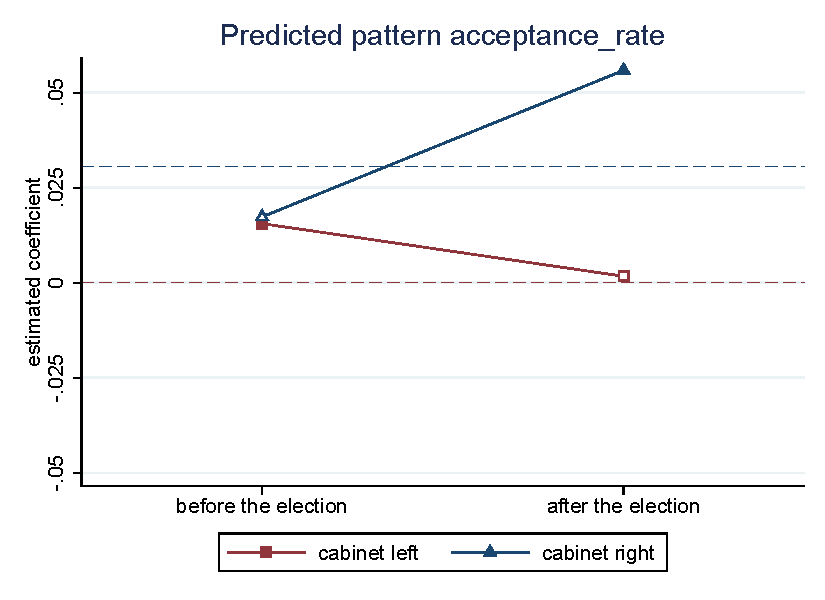
\includegraphics[width=1\textwidth]{figures_edited/acceptance_rate_graph1_R6.pdf}
	\caption{R6: Acceptance Rate: Predicted Pattern}
\end{figure}

\begin{table}[!ht]\centering
	\renewcommand{\arraystretch}{1.25}
	\def\sym#1{\ifmmode^{#1}\else\(^{#1}\)\fi}
	\caption{R6: Acceptance Rate: Predicted Pattern}
	\begin{tabular}{l*{2}{c}}
		\hline\hline
		                    &\multicolumn{1}{c}{(1)}&\multicolumn{1}{c}{(2)}\\
                    &\multicolumn{1}{c}{left}&\multicolumn{1}{c}{right}\\
\hline
before              &      0.0156\sym{*}  &     -0.0133         \\
                    &   (0.00618)         &   (0.00788)         \\
after               &     0.00173         &      0.0252\sym{***}\\
                    &   (0.00550)         &   (0.00539)         \\
\hline
Observations        &       17193         &       17193         \\

		\hline\hline
		\multicolumn{3}{c}{\footnotesize Standard errors in parentheses} \\
		\multicolumn{3}{c}{\footnotesize (\sym{*} \(p<0.05\), \sym{**} \(p<0.01\), \sym{***} \(p<0.001\))}\\
	\end{tabular}
\end{table}

\clearpage
\textbf{R6: Use Syrian battle death data from UCDP - Model 2}
\begin{figure}[!ht]
	\centering
	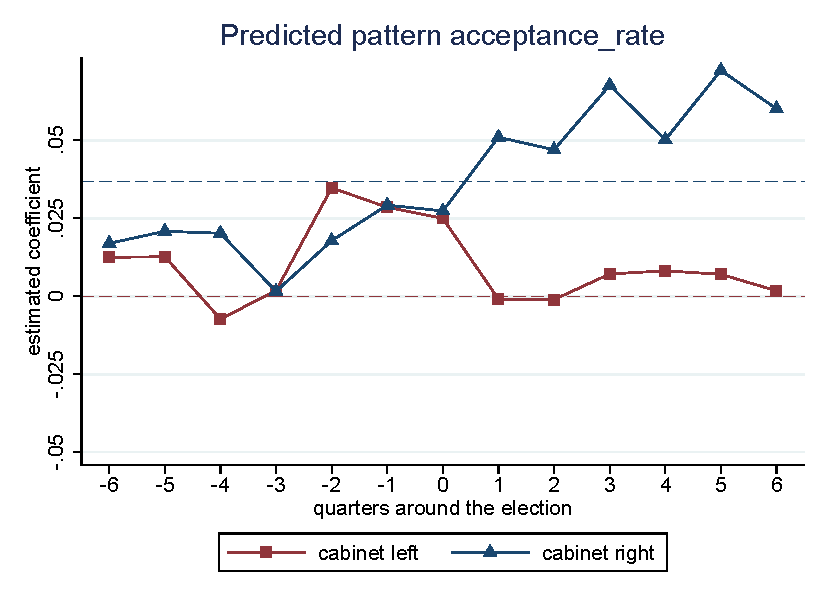
\includegraphics[width=0.7\textwidth]{figures_edited/acceptance_rate_graph2_R6.pdf}
	\caption{R6: Acceptance Rate: Predicted Pattern}
\end{figure}

\begin{table}[!ht]\centering
	\footnotesize
	\renewcommand{\arraystretch}{1.2}
	\def\sym#1{\ifmmode^{#1}\else\(^{#1}\)\fi}
	\caption{R6: Acceptance Rate: Predicted Pattern}
	\begin{tabular}{l*{2}{c}}
		\hline\hline
		                    &\multicolumn{1}{c}{(1)}&\multicolumn{1}{c}{(2)}\\
                    &\multicolumn{1}{c}{left}&\multicolumn{1}{c}{right}\\
\hline
 6 quarters before the election&      0.0125         &     -0.0199\sym{**} \\
                    &   (0.00988)         &   (0.00768)         \\
 5 quarters before the election&      0.0127         &     -0.0160         \\
                    &    (0.0105)         &   (0.00943)         \\
 4 quarters before the election&    -0.00732         &     -0.0166         \\
                    &   (0.00909)         &    (0.0107)         \\
 3 quarters before the election&     0.00181         &     -0.0353\sym{**} \\
                    &    (0.0133)         &    (0.0118)         \\
 2 quarters before the election&      0.0348\sym{***}&     -0.0190         \\
                    &   (0.00923)         &    (0.0110)         \\
 1 quarters before the election&      0.0285\sym{**} &    -0.00759         \\
                    &   (0.00963)         &    (0.0111)         \\
Quarter of the election&      0.0249\sym{**} &    -0.00948         \\
                    &   (0.00917)         &    (0.0142)         \\
 1 quarters after the election&   -0.000918         &      0.0142         \\
                    &   (0.00849)         &    (0.0123)         \\
 2 quarters after the election&    -0.00107         &      0.0101         \\
                    &   (0.00843)         &   (0.00915)         \\
 3 quarters after the election&     0.00712         &      0.0308\sym{**} \\
                    &   (0.00797)         &    (0.0104)         \\
 4 quarters after the election&     0.00816         &      0.0134         \\
                    &   (0.00811)         &   (0.00781)         \\
 5 quarters after the election&     0.00702         &      0.0356\sym{***}\\
                    &   (0.00825)         &    (0.0105)         \\
 6 quarters after the election&     0.00174         &      0.0233\sym{**} \\
                    &    (0.0105)         &   (0.00722)         \\
\hline
Observations        &       17193         &       17193         \\

		\hline\hline
		\multicolumn{3}{c}{\footnotesize Standard errors in parentheses} \\
		\multicolumn{3}{c}{\footnotesize (\sym{*} \(p<0.05\), \sym{**} \(p<0.01\), \sym{***} \(p<0.001\))} \\
	\end{tabular}
\end{table}


% ===============================================================================================================


\clearpage
\FloatBarrier
\subsubsection{Include a post 2007 dummy}
\begin{table}[!ht]\centering
	\renewcommand{\arraystretch}{1.25}
	\small
	\def\sym#1{\ifmmode^{#1}\else\(^{#1}\)\fi}
	\caption{R7: Determinants of acceptance rate}
	\begin{tabular}{l*{2}{c}}
		\hline\hline
		                                        &\multicolumn{1}{c}{(1)}         &\multicolumn{1}{c}{(2)}         \\
\hline
Political Terror Scale                  &    0.0167         &    0.0218\sym{*}  \\
                                        & (0.00984)         &  (0.0102)         \\
Civic Liberty (FHI)                     &    0.0405\sym{*}  &    0.0375         \\
                                        &  (0.0191)         &  (0.0192)         \\
Political Rights (FHI)                  &  -0.00987         &  -0.00808         \\
                                        &  (0.0150)         &  (0.0161)         \\
Quarterly civil war battle death (000s) &    0.0451\sym{***}&    0.0451\sym{***}\\
                                        & (0.00430)         & (0.00474)         \\
Log origin country real GDP per capita  &   -0.0166         &   -0.0200         \\
                                        &  (0.0315)         &  (0.0365)         \\
Log migrant stock in 2000/1             & -0.000750         &                   \\
                                        & (0.00240)         &                   \\
Log distance from origin to destination &    0.0142         &                   \\
                                        &  (0.0232)         &                   \\
Log destination country real GDP per capita&    0.0633         &    0.0934         \\
                                        &  (0.0686)         &  (0.0726)         \\
Quarterly unemployment rate at destination&  -0.00121         &  -0.00119         \\
                                        & (0.00126)         & (0.00116)         \\
Log average past total asylum decisions per capita&    -160.2\sym{***}&    -168.9\sym{***}\\
                                        &   (36.15)         &   (37.45)         \\
Log average past dyadic asylum decisions per capita&     418.9\sym{*}  &     295.9         \\
                                        &   (196.0)         &   (228.6)         \\
after 2007                              &     0.159\sym{***}&    0.0180         \\
                                        &  (0.0402)         &  (0.0278)         \\
Weighted cabinet position right         &    0.0283\sym{*}  &    0.0309\sym{**} \\
                                        &  (0.0108)         &  (0.0111)         \\
Cabinet position left * Before the election&    0.0125\sym{*}  &    0.0158\sym{*}  \\
                                        & (0.00609)         & (0.00608)         \\
Cabinet position left * After the election&   0.00194         &   0.00186         \\
                                        & (0.00519)         & (0.00548)         \\
Cabinet position right * Before the election&   -0.0121         &   -0.0131         \\
                                        & (0.00808)         & (0.00789)         \\
Cabinet position right * After the election&    0.0270\sym{***}&    0.0251\sym{***}\\
                                        & (0.00567)         & (0.00538)         \\
\hline
Observations                            &     17193         &     17193         \\
Adjusted \(R^{2}\)                      &     0.156         &     0.106         \\
Fixed Effects                           &         O         &     D x O         \\
Destination dummies                     &       Yes         &        No         \\
Quarter-Year dummies                    &       Yes         &       Yes         \\

		\hline\hline
		\multicolumn{3}{l}{\footnotesize Standard errors in parentheses (\sym{*} \(p<0.05\), \sym{**} \(p<0.01\), \sym{***} \(p<0.001\))}\\
	\end{tabular}
\end{table}

\clearpage
\textbf{R7: Include a post 2007 dummy - Model 1}
\begin{figure}[!ht]
	\centering
	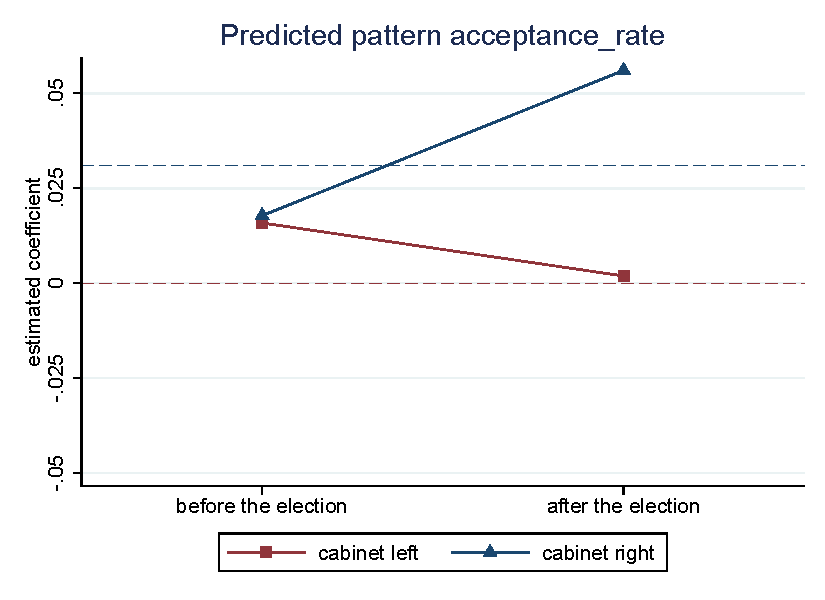
\includegraphics[width=1\textwidth]{figures_edited/acceptance_rate_graph1_R7.pdf}
	\caption{R7: Acceptance Rate: Predicted Pattern}
\end{figure}

\begin{table}[!ht]\centering
	\renewcommand{\arraystretch}{1.25}
	\def\sym#1{\ifmmode^{#1}\else\(^{#1}\)\fi}
	\caption{R7: Acceptance Rate: Predicted Pattern}
	\begin{tabular}{l*{2}{c}}
		\hline\hline
		                    &\multicolumn{1}{c}{(1)}&\multicolumn{1}{c}{(2)}\\
                    &\multicolumn{1}{c}{left}&\multicolumn{1}{c}{right}\\
\hline
before              &      0.0158\sym{**} &     -0.0131         \\
                    &   (0.00608)         &   (0.00789)         \\
after               &     0.00186         &      0.0251\sym{***}\\
                    &   (0.00548)         &   (0.00538)         \\
\hline
Observations        &       17193         &       17193         \\

		\hline\hline
		\multicolumn{3}{c}{\footnotesize Standard errors in parentheses} \\
		\multicolumn{3}{c}{\footnotesize (\sym{*} \(p<0.05\), \sym{**} \(p<0.01\), \sym{***} \(p<0.001\))}\\
	\end{tabular}
\end{table}

\clearpage
\textbf{R7: Include a post 2007 dummy - Model 2}
\begin{figure}[!ht]
	\centering
	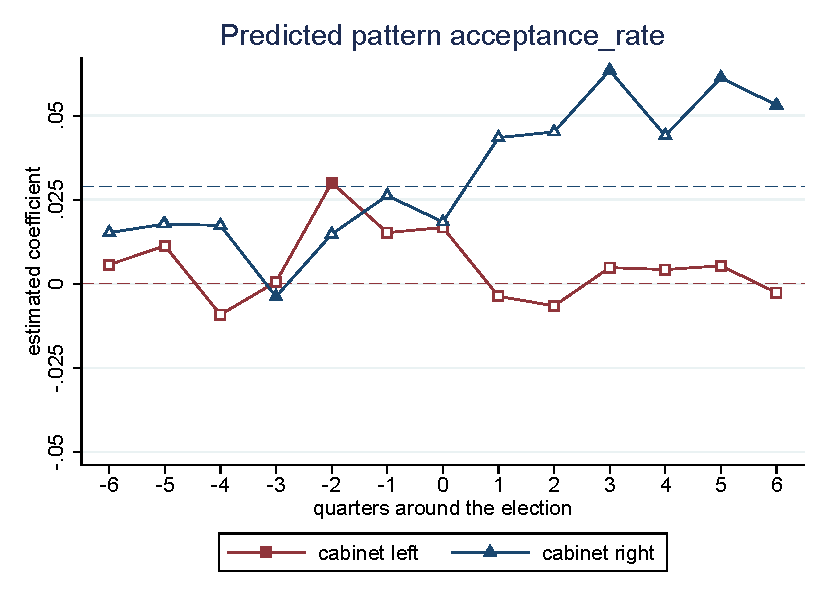
\includegraphics[width=0.7\textwidth]{figures_edited/acceptance_rate_graph2_R7.pdf}
	\caption{R7: Acceptance Rate: Predicted Pattern}
\end{figure}

\begin{table}[!ht]\centering
	\footnotesize
	\renewcommand{\arraystretch}{1.2}
	\def\sym#1{\ifmmode^{#1}\else\(^{#1}\)\fi}
	\caption{R7: Acceptance Rate: Predicted Pattern}
	\begin{tabular}{l*{2}{c}}
		\hline\hline
		                    &\multicolumn{1}{c}{(1)}&\multicolumn{1}{c}{(2)}\\
                    &\multicolumn{1}{c}{left}&\multicolumn{1}{c}{right}\\
\hline
 6 quarters before the election&      0.0123         &     -0.0197\sym{**} \\
                    &   (0.00990)         &   (0.00762)         \\
 5 quarters before the election&      0.0129         &     -0.0158         \\
                    &    (0.0104)         &   (0.00942)         \\
 4 quarters before the election&    -0.00712         &     -0.0164         \\
                    &   (0.00908)         &    (0.0108)         \\
 3 quarters before the election&     0.00230         &     -0.0352\sym{**} \\
                    &    (0.0133)         &    (0.0118)         \\
 2 quarters before the election&      0.0351\sym{***}&     -0.0188         \\
                    &   (0.00912)         &    (0.0110)         \\
 1 quarters before the election&      0.0287\sym{**} &    -0.00748         \\
                    &   (0.00961)         &    (0.0111)         \\
Quarter of the election&      0.0250\sym{**} &    -0.00918         \\
                    &   (0.00914)         &    (0.0142)         \\
 1 quarters after the election&   -0.000750         &      0.0143         \\
                    &   (0.00845)         &    (0.0122)         \\
 2 quarters after the election&   -0.000748         &      0.0101         \\
                    &   (0.00856)         &   (0.00915)         \\
 3 quarters after the election&     0.00738         &      0.0306\sym{**} \\
                    &   (0.00800)         &    (0.0104)         \\
 4 quarters after the election&     0.00828         &      0.0134         \\
                    &   (0.00807)         &   (0.00775)         \\
 5 quarters after the election&     0.00698         &      0.0354\sym{***}\\
                    &   (0.00821)         &    (0.0105)         \\
 6 quarters after the election&     0.00155         &      0.0231\sym{**} \\
                    &    (0.0105)         &   (0.00717)         \\
\hline
Observations        &       17193         &       17193         \\

		\hline\hline
		\multicolumn{3}{c}{\footnotesize Standard errors in parentheses} \\
		\multicolumn{3}{c}{\footnotesize (\sym{*} \(p<0.05\), \sym{**} \(p<0.01\), \sym{***} \(p<0.001\))} \\
	\end{tabular}
\end{table}


% ===============================================================================================================


\clearpage
\FloatBarrier
\subsubsection{Cluster standard errors on destination*origin level}
\textbf{R8: Cluster standard errors on destination*origin level - Model 1}
\begin{figure}[!ht]
	\centering
	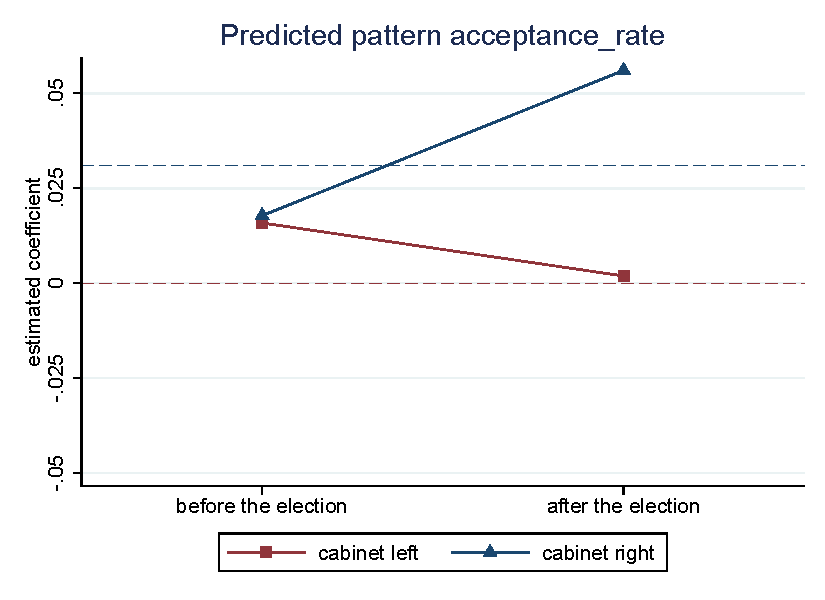
\includegraphics[width=1\textwidth]{figures_edited/acceptance_rate_graph1_R8.pdf}
	\caption{R8: Acceptance Rate: Predicted Pattern}
\end{figure}

\begin{table}[!ht]\centering
	\renewcommand{\arraystretch}{1.25}
	\def\sym#1{\ifmmode^{#1}\else\(^{#1}\)\fi}
	\caption{R8: Acceptance Rate: Predicted Pattern}
	\begin{tabular}{l*{2}{c}}
		\hline\hline
		                    &\multicolumn{1}{c}{(1)}&\multicolumn{1}{c}{(2)}\\
                    &\multicolumn{1}{c}{left}&\multicolumn{1}{c}{right}\\
\hline
before              &      0.0158\sym{*}  &     -0.0131\sym{*}  \\
                    &   (0.00684)         &   (0.00639)         \\
after               &     0.00186         &      0.0251\sym{***}\\
                    &   (0.00569)         &   (0.00648)         \\
\hline
Observations        &       17193         &       17193         \\

		\hline\hline
		\multicolumn{3}{c}{\footnotesize Standard errors in parentheses} \\
		\multicolumn{3}{c}{\footnotesize (\sym{*} \(p<0.05\), \sym{**} \(p<0.01\), \sym{***} \(p<0.001\))}\\
	\end{tabular}
\end{table}

\clearpage
\textbf{R8: Cluster standard errors on destination*origin level - Model 2}
\begin{figure}[!ht]
	\centering
	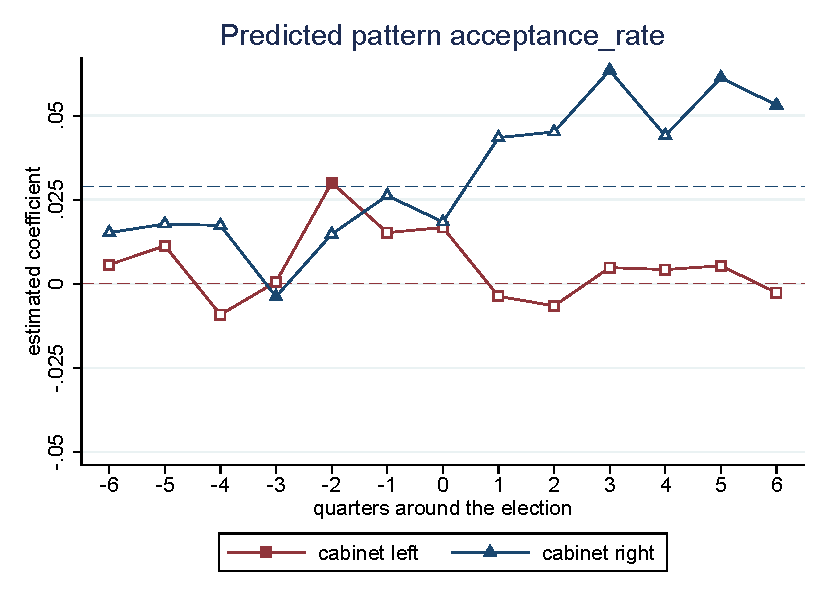
\includegraphics[width=0.7\textwidth]{figures_edited/acceptance_rate_graph2_R8.pdf}
	\caption{R8: Acceptance Rate: Predicted Pattern}
\end{figure}

\begin{table}[!ht]\centering
	\footnotesize
	\renewcommand{\arraystretch}{1.2}
	\def\sym#1{\ifmmode^{#1}\else\(^{#1}\)\fi}
	\caption{R8: Acceptance Rate: Predicted Pattern}
	\begin{tabular}{l*{2}{c}}
		\hline\hline
		                    &\multicolumn{1}{c}{(1)}&\multicolumn{1}{c}{(2)}\\
                    &\multicolumn{1}{c}{left}&\multicolumn{1}{c}{right}\\
\hline
 6 quarters before the election&      0.0123         &     -0.0197\sym{*}  \\
                    &   (0.00933)         &   (0.00886)         \\
 5 quarters before the election&      0.0129         &     -0.0158         \\
                    &   (0.00978)         &   (0.00990)         \\
 4 quarters before the election&    -0.00712         &     -0.0164         \\
                    &    (0.0113)         &   (0.00991)         \\
 3 quarters before the election&     0.00230         &     -0.0352\sym{***}\\
                    &    (0.0127)         &    (0.0100)         \\
 2 quarters before the election&      0.0351\sym{**} &     -0.0188         \\
                    &    (0.0113)         &    (0.0117)         \\
 1 quarters before the election&      0.0287\sym{**} &    -0.00748         \\
                    &    (0.0105)         &    (0.0105)         \\
Quarter of the election&      0.0250\sym{**} &    -0.00918         \\
                    &   (0.00971)         &    (0.0108)         \\
 1 quarters after the election&   -0.000750         &      0.0143         \\
                    &   (0.00902)         &    (0.0112)         \\
 2 quarters after the election&   -0.000748         &      0.0101         \\
                    &   (0.00892)         &    (0.0116)         \\
 3 quarters after the election&     0.00738         &      0.0306\sym{**} \\
                    &   (0.00865)         &    (0.0104)         \\
 4 quarters after the election&     0.00828         &      0.0134         \\
                    &   (0.00928)         &    (0.0101)         \\
 5 quarters after the election&     0.00698         &      0.0354\sym{***}\\
                    &   (0.00801)         &    (0.0100)         \\
 6 quarters after the election&     0.00155         &      0.0231\sym{*}  \\
                    &   (0.00846)         &   (0.00980)         \\
\hline
Observations        &       17193         &       17193         \\

		\hline\hline
		\multicolumn{3}{c}{\footnotesize Standard errors in parentheses} \\
		\multicolumn{3}{c}{\footnotesize (\sym{*} \(p<0.05\), \sym{**} \(p<0.01\), \sym{***} \(p<0.001\))} \\
	\end{tabular}
\end{table}



% ===============================================================================================================


\clearpage
\FloatBarrier
\subsubsection{Drop country pairs with less than one decision per quarter on average}
\begin{table}[!ht]\centering
	\renewcommand{\arraystretch}{1.25}
	\small
	\def\sym#1{\ifmmode^{#1}\else\(^{#1}\)\fi}
	\caption{R9: Determinants of acceptance rate}
	\begin{tabular}{l*{3}{c}}
		\hline\hline
		                                        &\multicolumn{1}{c}{(1)}         &\multicolumn{1}{c}{(2)}         &\multicolumn{1}{c}{(3)}         \\
\hline
Political Terror Scale                  &    0.0168         &    0.0224\sym{*}  &                   \\
                                        & (0.00994)         &  (0.0103)         &                   \\
Civic Liberty (FHI)                     &    0.0382         &    0.0360         &                   \\
                                        &  (0.0192)         &  (0.0191)         &                   \\
Political Rights (FHI)                  &  -0.00927         &  -0.00797         &                   \\
                                        &  (0.0148)         &  (0.0161)         &                   \\
Quarterly civil war battle death (000s) &    0.0452\sym{***}&    0.0451\sym{***}&                   \\
                                        & (0.00434)         & (0.00477)         &                   \\
Log origin country real GDP per capita  &   -0.0157         &   -0.0205         &                   \\
                                        &  (0.0322)         &  (0.0368)         &                   \\
Log migrant stock in 2000/1             & -0.000906         &                   & -0.000402         \\
                                        & (0.00235)         &                   & (0.00238)         \\
Log distance from origin to destination &    0.0114         &                   &    0.0132         \\
                                        &  (0.0223)         &                   &  (0.0229)         \\
Log destination country real GDP per capita&    0.0787         &     0.100         &    0.0786         \\
                                        &  (0.0706)         &  (0.0727)         &  (0.0697)         \\
Quarterly unemployment rate at destination&  -0.00105         & -0.000994         &  -0.00118         \\
                                        & (0.00122)         & (0.00110)         & (0.00126)         \\
Log average past total asylum decisions per capita&    -165.2\sym{***}&    -169.7\sym{***}&    -161.9\sym{***}\\
                                        &   (35.74)         &   (37.08)         &   (37.44)         \\
Log average past dyadic asylum decisions per capita&     432.1\sym{*}  &     296.8         &     277.9         \\
                                        &   (196.6)         &   (227.5)         &   (209.8)         \\
Weighted cabinet position right         &    0.0291\sym{**} &    0.0313\sym{**} &    0.0278\sym{*}  \\
                                        &  (0.0106)         &  (0.0108)         &  (0.0110)         \\
Cabinet position left * Before the election&    0.0113         &    0.0145\sym{*}  &    0.0112         \\
                                        & (0.00607)         & (0.00603)         & (0.00638)         \\
Cabinet position left * After the election&   0.00206         &   0.00182         &   0.00226         \\
                                        & (0.00498)         & (0.00525)         & (0.00534)         \\
Cabinet position right * Before the election&   -0.0142         &   -0.0145         &   -0.0128         \\
                                        & (0.00835)         & (0.00788)         & (0.00842)         \\
Cabinet position right * After the election&    0.0244\sym{***}&    0.0226\sym{***}&    0.0237\sym{***}\\
                                        & (0.00592)         & (0.00558)         & (0.00613)         \\
\hline
Observations                            &     17604         &     17604         &     17604         \\
Adjusted \(R^{2}\)                      &     0.152         &     0.103         &     0.101         \\
Fixed Effects                           &         O         &     D x O         &     O x T         \\
Destination dummies                     &       Yes         &        No         &       Yes         \\
Quarter-Year dummies                    &       Yes         &       Yes         &        No         \\

		\hline\hline
		\multicolumn{4}{l}{\footnotesize Standard errors in parentheses (\sym{*} \(p<0.05\), \sym{**} \(p<0.01\), \sym{***} \(p<0.001\))}\\
	\end{tabular}
\end{table}

\clearpage
\textbf{R9: Drop country pairs with less than one decision per quarter on average - Model 1}
\begin{figure}[!ht]
	\centering
	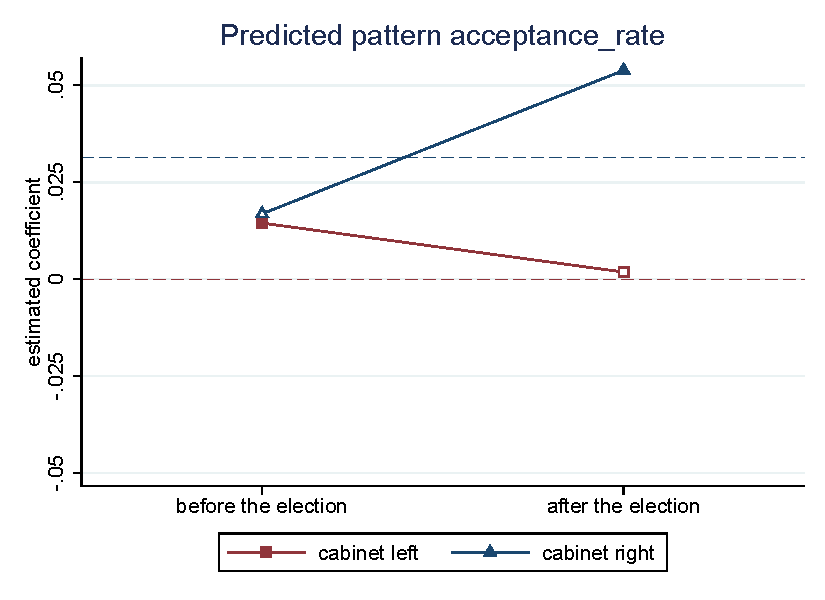
\includegraphics[width=1\textwidth]{figures_edited/acceptance_rate_graph1_R9.pdf}
	\caption{R9: Acceptance Rate: Predicted Pattern}
\end{figure}

\begin{table}[!ht]\centering
	\renewcommand{\arraystretch}{1.25}
	\def\sym#1{\ifmmode^{#1}\else\(^{#1}\)\fi}
	\caption{R9: Acceptance Rate: Predicted Pattern}
	\begin{tabular}{l*{2}{c}}
		\hline\hline
		                    &\multicolumn{1}{c}{(1)}&\multicolumn{1}{c}{(2)}\\
                    &\multicolumn{1}{c}{left}&\multicolumn{1}{c}{right}\\
\hline
before              &      0.0145\sym{*}  &     -0.0145         \\
                    &   (0.00603)         &   (0.00788)         \\
after               &     0.00182         &      0.0226\sym{***}\\
                    &   (0.00525)         &   (0.00558)         \\
\hline
Observations        &       17604         &       17604         \\

		\hline\hline
		\multicolumn{3}{c}{\footnotesize Standard errors in parentheses} \\
		\multicolumn{3}{c}{\footnotesize (\sym{*} \(p<0.05\), \sym{**} \(p<0.01\), \sym{***} \(p<0.001\))}\\
	\end{tabular}
\end{table}

\clearpage
\textbf{R9: Drop country pairs with less than one decision per quarter on average - Model 2}
\begin{figure}[!ht]
	\centering
	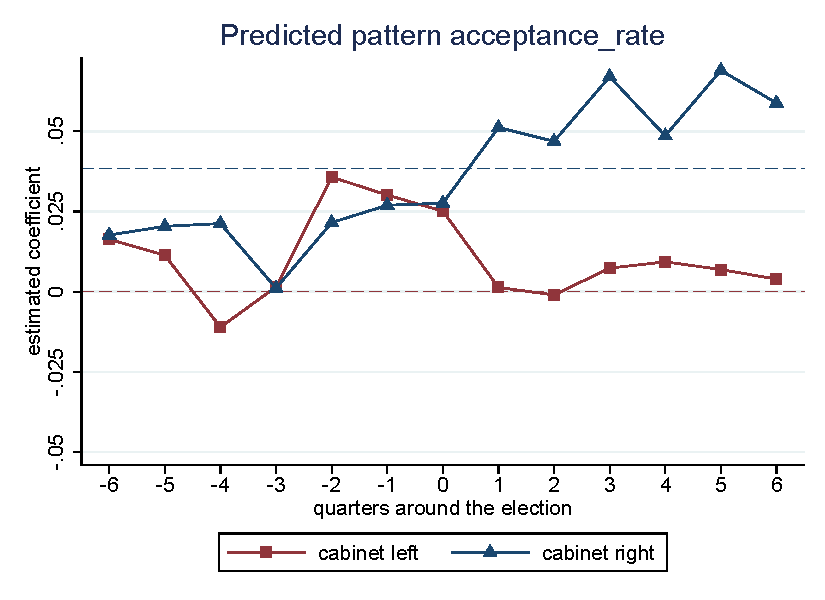
\includegraphics[width=0.7\textwidth]{figures_edited/acceptance_rate_graph2_R9.pdf}
	\caption{R9: Acceptance Rate: Predicted Pattern}
\end{figure}

\begin{table}[!ht]\centering
	\footnotesize
	\renewcommand{\arraystretch}{1.2}
	\def\sym#1{\ifmmode^{#1}\else\(^{#1}\)\fi}
	\caption{R9: Acceptance Rate: Predicted Pattern}
	\begin{tabular}{l*{2}{c}}
		\hline\hline
		                    &\multicolumn{1}{c}{(1)}&\multicolumn{1}{c}{(2)}\\
                    &\multicolumn{1}{c}{left}&\multicolumn{1}{c}{right}\\
\hline
 6 quarters before the election&      0.0163         &     -0.0208\sym{**} \\
                    &    (0.0106)         &   (0.00742)         \\
 5 quarters before the election&      0.0114         &     -0.0181         \\
                    &   (0.01000)         &   (0.00929)         \\
 4 quarters before the election&     -0.0111         &     -0.0172         \\
                    &   (0.00868)         &    (0.0110)         \\
 3 quarters before the election&     0.00151         &     -0.0373\sym{**} \\
                    &    (0.0132)         &    (0.0115)         \\
 2 quarters before the election&      0.0357\sym{***}&     -0.0169         \\
                    &   (0.00925)         &    (0.0111)         \\
 1 quarters before the election&      0.0301\sym{**} &     -0.0115         \\
                    &   (0.00964)         &    (0.0111)         \\
Quarter of the election&      0.0251\sym{**} &     -0.0108         \\
                    &   (0.00918)         &    (0.0139)         \\
 1 quarters after the election&     0.00133         &      0.0128         \\
                    &   (0.00814)         &    (0.0121)         \\
 2 quarters after the election&    -0.00101         &     0.00845         \\
                    &   (0.00835)         &   (0.00995)         \\
 3 quarters after the election&     0.00735         &      0.0286\sym{**} \\
                    &   (0.00804)         &    (0.0107)         \\
 4 quarters after the election&     0.00932         &      0.0102         \\
                    &   (0.00824)         &   (0.00772)         \\
 5 quarters after the election&     0.00692         &      0.0306\sym{**} \\
                    &   (0.00782)         &    (0.0105)         \\
 6 quarters after the election&     0.00392         &      0.0204\sym{**} \\
                    &    (0.0101)         &   (0.00733)         \\
\hline
Observations        &       17604         &       17604         \\

		\hline\hline
		\multicolumn{3}{c}{\footnotesize Standard errors in parentheses} \\
		\multicolumn{3}{c}{\footnotesize (\sym{*} \(p<0.05\), \sym{**} \(p<0.01\), \sym{***} \(p<0.001\))} \\
	\end{tabular}
\end{table}



% ===============================================================================================================


\clearpage
\FloatBarrier
\subsubsection{Drop country pairs with less than three decisions per quarter on average}
\begin{table}[!ht]\centering
	\renewcommand{\arraystretch}{1.25}
	\small
	\def\sym#1{\ifmmode^{#1}\else\(^{#1}\)\fi}
	\caption{R10: Determinants of acceptance rate}
	\begin{tabular}{l*{3}{c}}
		\hline\hline
		                                        &\multicolumn{1}{c}{(1)}         &\multicolumn{1}{c}{(2)}         &\multicolumn{1}{c}{(3)}         \\
\hline
Political Terror Scale                  &    0.0172         &    0.0213\sym{*}  &                   \\
                                        & (0.00959)         & (0.00965)         &                   \\
Civic Liberty (FHI)                     &    0.0398\sym{*}  &    0.0367         &                   \\
                                        &  (0.0196)         &  (0.0193)         &                   \\
Political Rights (FHI)                  &  -0.00816         &  -0.00649         &                   \\
                                        &  (0.0149)         &  (0.0163)         &                   \\
Quarterly civil war battle death (000s) &    0.0431\sym{***}&    0.0435\sym{***}&                   \\
                                        & (0.00417)         & (0.00454)         &                   \\
Log origin country real GDP per capita  &   -0.0226         &   -0.0240         &                   \\
                                        &  (0.0318)         &  (0.0369)         &                   \\
Log migrant stock in 2000/1             & -0.000794         &                   & -0.000377         \\
                                        & (0.00255)         &                   & (0.00258)         \\
Log distance from origin to destination &    0.0145         &                   &    0.0161         \\
                                        &  (0.0223)         &                   &  (0.0226)         \\
Log destination country real GDP per capita&    0.0517         &    0.0716         &    0.0558         \\
                                        &  (0.0709)         &  (0.0733)         &  (0.0681)         \\
Quarterly unemployment rate at destination&  -0.00137         &  -0.00151         &  -0.00166         \\
                                        & (0.00125)         & (0.00118)         & (0.00131)         \\
Log average past total asylum decisions per capita&    -140.7\sym{***}&    -151.9\sym{***}&    -138.1\sym{***}\\
                                        &   (35.66)         &   (38.01)         &   (37.02)         \\
Log average past dyadic asylum decisions per capita&     427.6\sym{*}  &     287.2         &     282.7         \\
                                        &   (202.2)         &   (235.1)         &   (215.9)         \\
Weighted cabinet position right         &    0.0294\sym{**} &    0.0299\sym{**} &    0.0258\sym{*}  \\
                                        &  (0.0108)         &  (0.0109)         &  (0.0111)         \\
Cabinet position left * Before the election&    0.0146\sym{*}  &    0.0160\sym{**} &    0.0127\sym{*}  \\
                                        & (0.00571)         & (0.00572)         & (0.00582)         \\
Cabinet position left * After the election&   0.00359         &   0.00229         &   0.00242         \\
                                        & (0.00563)         & (0.00571)         & (0.00589)         \\
Cabinet position right * Before the election&   -0.0105         &   -0.0113         &  -0.00842         \\
                                        & (0.00753)         & (0.00746)         & (0.00775)         \\
Cabinet position right * After the election&    0.0267\sym{***}&    0.0252\sym{***}&    0.0270\sym{***}\\
                                        & (0.00584)         & (0.00558)         & (0.00595)         \\
\hline
Observations                            &     16594         &     16594         &     16594         \\
Adjusted \(R^{2}\)                      &     0.158         &     0.105         &     0.106         \\
Fixed Effects                           &         O         &     D x O         &     O x T         \\
Destination dummies                     &       Yes         &        No         &       Yes         \\
Quarter-Year dummies                    &       Yes         &       Yes         &        No         \\

		\hline\hline
		\multicolumn{4}{l}{\footnotesize Standard errors in parentheses (\sym{*} \(p<0.05\), \sym{**} \(p<0.01\), \sym{***} \(p<0.001\))}\\
	\end{tabular}
\end{table}

\clearpage
\textbf{R10: Drop country pairs with less than three decisions per quarter on average - Model 1}
\begin{figure}[!ht]
	\centering
	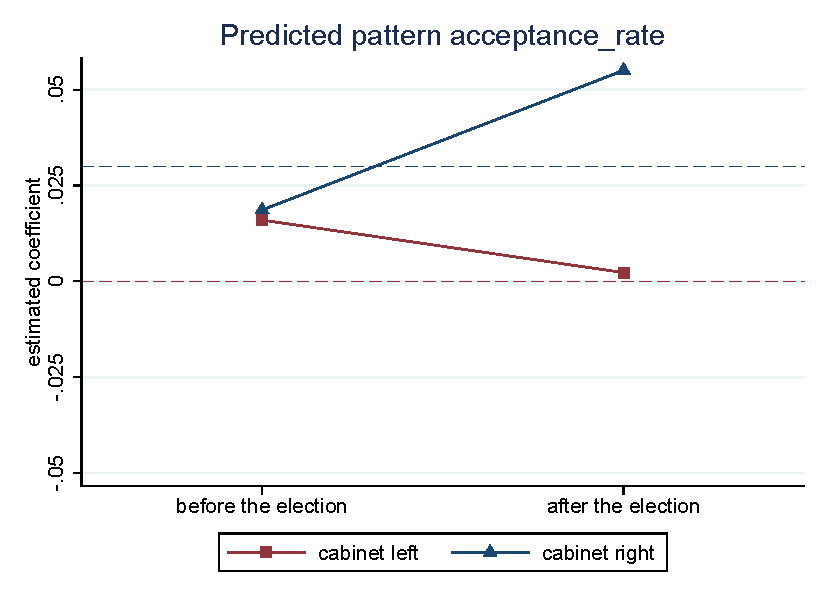
\includegraphics[width=1\textwidth]{figures_edited/acceptance_rate_graph1_R10.pdf}
	\caption{R10: Acceptance Rate: Predicted Pattern}
\end{figure}

\begin{table}[!ht]\centering
	\renewcommand{\arraystretch}{1.25}
	\def\sym#1{\ifmmode^{#1}\else\(^{#1}\)\fi}
	\caption{R10: Acceptance Rate: Predicted Pattern}
	\begin{tabular}{l*{2}{c}}
		\hline\hline
		                    &\multicolumn{1}{c}{(1)}&\multicolumn{1}{c}{(2)}\\
                    &\multicolumn{1}{c}{left}&\multicolumn{1}{c}{right}\\
\hline
before              &      0.0160\sym{**} &     -0.0113         \\
                    &   (0.00572)         &   (0.00746)         \\
after               &     0.00229         &      0.0252\sym{***}\\
                    &   (0.00571)         &   (0.00558)         \\
\hline
Observations        &       16594         &       16594         \\

		\hline\hline
		\multicolumn{3}{c}{\footnotesize Standard errors in parentheses} \\
		\multicolumn{3}{c}{\footnotesize (\sym{*} \(p<0.05\), \sym{**} \(p<0.01\), \sym{***} \(p<0.001\))}\\
	\end{tabular}
\end{table}

\clearpage
\textbf{R10: Drop country pairs with less than three decisions per quarter on average - Model 2}
\begin{figure}[!ht]
	\centering
	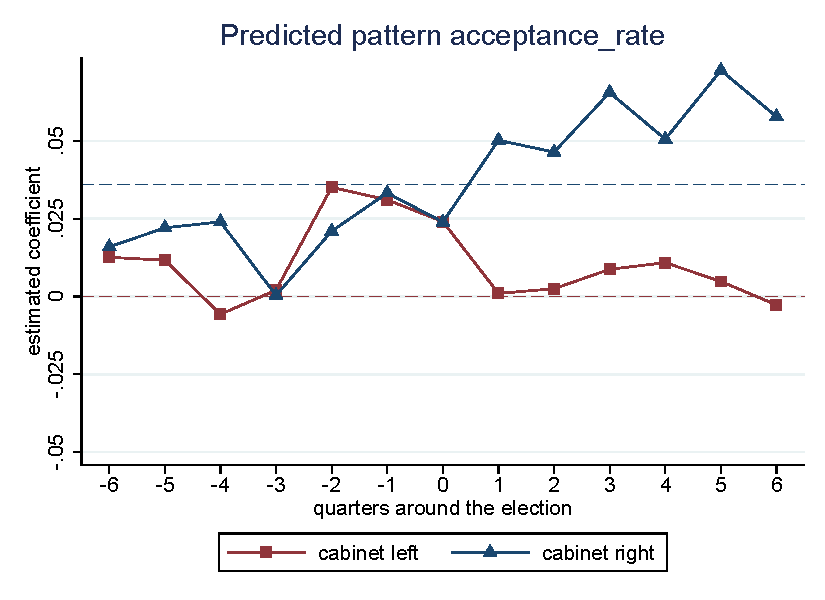
\includegraphics[width=0.7\textwidth]{figures_edited/acceptance_rate_graph2_R10.pdf}
	\caption{R10: Acceptance Rate: Predicted Pattern}
\end{figure}

\begin{table}[!ht]\centering
	\footnotesize
	\renewcommand{\arraystretch}{1.2}
	\def\sym#1{\ifmmode^{#1}\else\(^{#1}\)\fi}
	\caption{R10: Acceptance Rate: Predicted Pattern}
	\begin{tabular}{l*{2}{c}}
		\hline\hline
		                    &\multicolumn{1}{c}{(1)}&\multicolumn{1}{c}{(2)}\\
                    &\multicolumn{1}{c}{left}&\multicolumn{1}{c}{right}\\
\hline
 6 quarters before the election&      0.0126         &     -0.0202\sym{*}  \\
                    &    (0.0103)         &   (0.00831)         \\
 5 quarters before the election&      0.0117         &     -0.0141         \\
                    &    (0.0107)         &   (0.00968)         \\
 4 quarters before the election&    -0.00569         &     -0.0122         \\
                    &   (0.00989)         &    (0.0104)         \\
 3 quarters before the election&     0.00209         &     -0.0358\sym{**} \\
                    &    (0.0127)         &    (0.0115)         \\
 2 quarters before the election&      0.0351\sym{***}&     -0.0151         \\
                    &   (0.00783)         &    (0.0110)         \\
 1 quarters before the election&      0.0311\sym{**} &    -0.00288         \\
                    &   (0.00945)         &    (0.0108)         \\
Quarter of the election&      0.0241\sym{**} &     -0.0122         \\
                    &   (0.00914)         &    (0.0132)         \\
 1 quarters after the election&     0.00102         &      0.0141         \\
                    &   (0.00830)         &    (0.0115)         \\
 2 quarters after the election&     0.00252         &      0.0103         \\
                    &   (0.00907)         &   (0.00965)         \\
 3 quarters after the election&     0.00877         &      0.0294\sym{**} \\
                    &   (0.00857)         &    (0.0100)         \\
 4 quarters after the election&      0.0109         &      0.0144         \\
                    &   (0.00771)         &   (0.00777)         \\
 5 quarters after the election&     0.00485         &      0.0365\sym{***}\\
                    &   (0.00764)         &    (0.0106)         \\
 6 quarters after the election&    -0.00267         &      0.0217\sym{**} \\
                    &    (0.0107)         &   (0.00690)         \\
\hline
Observations        &       16594         &       16594         \\

		\hline\hline
		\multicolumn{3}{c}{\footnotesize Standard errors in parentheses} \\
		\multicolumn{3}{c}{\footnotesize (\sym{*} \(p<0.05\), \sym{**} \(p<0.01\), \sym{***} \(p<0.001\))} \\
	\end{tabular}
\end{table}



% ===============================================================================================================


\clearpage
\FloatBarrier
\subsubsection{Use normalized cabinet position to determine cabinet left-right dummies}
\begin{table}[!ht]\centering
	\renewcommand{\arraystretch}{1.25}
	\small
	\def\sym#1{\ifmmode^{#1}\else\(^{#1}\)\fi}
	\caption{R11: Determinants of acceptance rate}
	\begin{tabular}{l*{3}{c}}
		\hline\hline
		                                        &\multicolumn{1}{c}{(1)}         &\multicolumn{1}{c}{(2)}         &\multicolumn{1}{c}{(3)}         \\
\hline
Political Terror Scale                  &    0.0167         &    0.0218\sym{*}  &                   \\
                                        & (0.00984)         &  (0.0102)         &                   \\
Civic Liberty (FHI)                     &    0.0405\sym{*}  &    0.0375         &                   \\
                                        &  (0.0191)         &  (0.0192)         &                   \\
Political Rights (FHI)                  &  -0.00988         &  -0.00808         &                   \\
                                        &  (0.0150)         &  (0.0161)         &                   \\
Quarterly civil war battle death (000s) &    0.0451\sym{***}&    0.0451\sym{***}&                   \\
                                        & (0.00430)         & (0.00474)         &                   \\
Log origin country real GDP per capita  &   -0.0166         &   -0.0200         &                   \\
                                        &  (0.0315)         &  (0.0365)         &                   \\
Log migrant stock in 2000/1             & -0.000752         &                   & -0.000257         \\
                                        & (0.00240)         &                   & (0.00245)         \\
Log distance from origin to destination &    0.0142         &                   &    0.0153         \\
                                        &  (0.0232)         &                   &  (0.0235)         \\
Log destination country real GDP per capita&    0.0633         &    0.0933         &    0.0691         \\
                                        &  (0.0684)         &  (0.0724)         &  (0.0659)         \\
Quarterly unemployment rate at destination&  -0.00119         &  -0.00118         &  -0.00141         \\
                                        & (0.00126)         & (0.00116)         & (0.00129)         \\
Log average past total asylum decisions per capita&    -160.2\sym{***}&    -169.0\sym{***}&    -159.1\sym{***}\\
                                        &   (36.11)         &   (37.43)         &   (37.78)         \\
Log average past dyadic asylum decisions per capita&     419.0\sym{*}  &     296.0         &     272.6         \\
                                        &   (196.0)         &   (228.7)         &   (208.9)         \\
Weighted cabinet position right         &    0.0283\sym{*}  &    0.0309\sym{**} &    0.0269\sym{*}  \\
                                        &  (0.0108)         &  (0.0111)         &  (0.0112)         \\
Cabinet position left * Before the election&    0.0118         &    0.0154\sym{*}  &    0.0107         \\
                                        & (0.00608)         & (0.00609)         & (0.00623)         \\
Cabinet position left * After the election&   0.00195         &   0.00187         &   0.00198         \\
                                        & (0.00519)         & (0.00549)         & (0.00556)         \\
Cabinet position right * Before the election&   -0.0114         &   -0.0126         &  -0.00985         \\
                                        & (0.00814)         & (0.00794)         & (0.00820)         \\
Cabinet position right * After the election&    0.0270\sym{***}&    0.0251\sym{***}&    0.0263\sym{***}\\
                                        & (0.00567)         & (0.00538)         & (0.00589)         \\
\hline
Observations                            &     17193         &     17193         &     17193         \\
Adjusted \(R^{2}\)                      &     0.156         &     0.106         &     0.104         \\
Fixed Effects                           &         O         &     D x O         &     O x T         \\
Destination dummies                     &       Yes         &        No         &       Yes         \\
Quarter-Year dummies                    &       Yes         &       Yes         &        No         \\

		\hline\hline
		\multicolumn{4}{l}{\footnotesize Standard errors in parentheses (\sym{*} \(p<0.05\), \sym{**} \(p<0.01\), \sym{***} \(p<0.001\))}\\
	\end{tabular}
\end{table}

\clearpage
\textbf{R11: Use normalized cabinet position to determine cabinet left-right dummies - Model 1}
\begin{figure}[!ht]
	\centering
	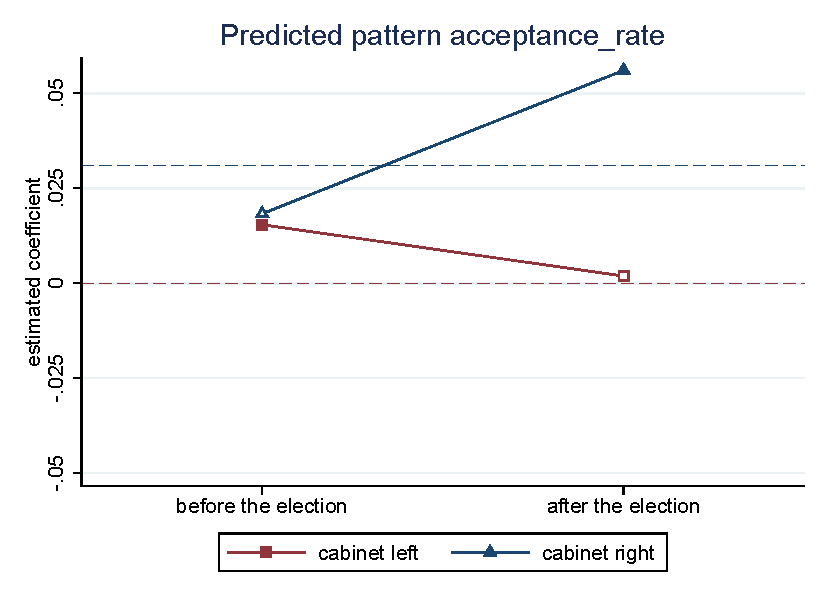
\includegraphics[width=1\textwidth]{figures_edited/acceptance_rate_graph1_R11.pdf}
	\caption{R11: Acceptance Rate: Predicted Pattern}
\end{figure}

\begin{table}[!ht]\centering
	\renewcommand{\arraystretch}{1.25}
	\def\sym#1{\ifmmode^{#1}\else\(^{#1}\)\fi}
	\caption{R11: Acceptance Rate: Predicted Pattern}
	\begin{tabular}{l*{2}{c}}
		\hline\hline
		                    &\multicolumn{1}{c}{(1)}&\multicolumn{1}{c}{(2)}\\
                    &\multicolumn{1}{c}{left}&\multicolumn{1}{c}{right}\\
\hline
before              &      0.0154\sym{*}  &     -0.0126         \\
                    &   (0.00609)         &   (0.00794)         \\
after               &     0.00187         &      0.0251\sym{***}\\
                    &   (0.00549)         &   (0.00538)         \\
\hline
Observations        &       17193         &       17193         \\

		\hline\hline
		\multicolumn{3}{c}{\footnotesize Standard errors in parentheses} \\
		\multicolumn{3}{c}{\footnotesize (\sym{*} \(p<0.05\), \sym{**} \(p<0.01\), \sym{***} \(p<0.001\))}\\
	\end{tabular}
\end{table}

\clearpage
\textbf{R11: Use normalized cabinet position to determine cabinet left-right dummies - Model 2}
\begin{figure}[!ht]
	\centering
	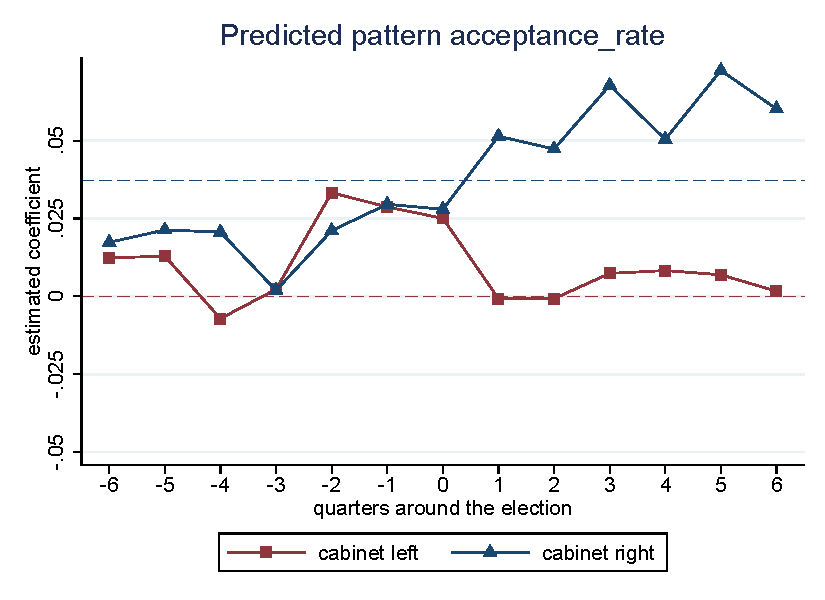
\includegraphics[width=0.7\textwidth]{figures_edited/acceptance_rate_graph2_R11.pdf}
	\caption{R11: Acceptance Rate: Predicted Pattern}
\end{figure}

\begin{table}[!ht]\centering
	\footnotesize
	\renewcommand{\arraystretch}{1.2}
	\def\sym#1{\ifmmode^{#1}\else\(^{#1}\)\fi}
	\caption{R11: Acceptance Rate: Predicted Pattern}
	\begin{tabular}{l*{2}{c}}
		\hline\hline
		                    &\multicolumn{1}{c}{(1)}&\multicolumn{1}{c}{(2)}\\
                    &\multicolumn{1}{c}{left}&\multicolumn{1}{c}{right}\\
\hline
 6 quarters before the election&      0.0123         &     -0.0197\sym{**} \\
                    &   (0.00989)         &   (0.00762)         \\
 5 quarters before the election&      0.0129         &     -0.0158         \\
                    &    (0.0104)         &   (0.00943)         \\
 4 quarters before the election&    -0.00714         &     -0.0164         \\
                    &   (0.00907)         &    (0.0108)         \\
 3 quarters before the election&     0.00228         &     -0.0351\sym{**} \\
                    &    (0.0133)         &    (0.0118)         \\
 2 quarters before the election&      0.0333\sym{***}&     -0.0160         \\
                    &   (0.00835)         &    (0.0113)         \\
 1 quarters before the election&      0.0287\sym{**} &    -0.00751         \\
                    &   (0.00960)         &    (0.0111)         \\
Quarter of the election&      0.0250\sym{**} &    -0.00913         \\
                    &   (0.00914)         &    (0.0142)         \\
 1 quarters after the election&   -0.000737         &      0.0143         \\
                    &   (0.00846)         &    (0.0122)         \\
 2 quarters after the election&   -0.000729         &      0.0102         \\
                    &   (0.00855)         &   (0.00913)         \\
 3 quarters after the election&     0.00736         &      0.0306\sym{**} \\
                    &   (0.00798)         &    (0.0104)         \\
 4 quarters after the election&     0.00829         &      0.0133         \\
                    &   (0.00807)         &   (0.00775)         \\
 5 quarters after the election&     0.00692         &      0.0355\sym{***}\\
                    &   (0.00826)         &    (0.0105)         \\
 6 quarters after the election&     0.00165         &      0.0231\sym{**} \\
                    &    (0.0105)         &   (0.00718)         \\
\hline
Observations        &       17193         &       17193         \\

		\hline\hline
		\multicolumn{3}{c}{\footnotesize Standard errors in parentheses} \\
		\multicolumn{3}{c}{\footnotesize (\sym{*} \(p<0.05\), \sym{**} \(p<0.01\), \sym{***} \(p<0.001\))} \\
	\end{tabular}
\end{table}



% ===============================================================================================================


\clearpage
\FloatBarrier
\subsubsection{Split cabinet position at 5 to determine cabinet left-right dummies}
\begin{table}[!ht]\centering
	\renewcommand{\arraystretch}{1.25}
	\small
	\def\sym#1{\ifmmode^{#1}\else\(^{#1}\)\fi}
	\caption{R12: Determinants of acceptance rate}
	\begin{tabular}{l*{3}{c}}
		\hline\hline
		                                        &\multicolumn{1}{c}{(1)}         &\multicolumn{1}{c}{(2)}         &\multicolumn{1}{c}{(3)}         \\
\hline
Political Terror Scale                  &    0.0171         &    0.0222\sym{*}  &                   \\
                                        & (0.00989)         &  (0.0103)         &                   \\
Civic Liberty (FHI)                     &    0.0406\sym{*}  &    0.0376         &                   \\
                                        &  (0.0190)         &  (0.0191)         &                   \\
Political Rights (FHI)                  &  -0.00993         &  -0.00819         &                   \\
                                        &  (0.0149)         &  (0.0161)         &                   \\
Quarterly civil war battle death (000s) &    0.0450\sym{***}&    0.0451\sym{***}&                   \\
                                        & (0.00431)         & (0.00474)         &                   \\
Log origin country real GDP per capita  &   -0.0169         &   -0.0204         &                   \\
                                        &  (0.0317)         &  (0.0367)         &                   \\
Log migrant stock in 2000/1             & -0.000707         &                   & -0.000200         \\
                                        & (0.00240)         &                   & (0.00245)         \\
Log distance from origin to destination &    0.0144         &                   &    0.0155         \\
                                        &  (0.0232)         &                   &  (0.0235)         \\
Log destination country real GDP per capita&    0.0766         &     0.106         &    0.0814         \\
                                        &  (0.0701)         &  (0.0742)         &  (0.0670)         \\
Quarterly unemployment rate at destination& -0.000730         & -0.000679         &  -0.00100         \\
                                        & (0.00129)         & (0.00120)         & (0.00132)         \\
Log average past total asylum decisions per capita&    -162.4\sym{***}&    -170.9\sym{***}&    -161.0\sym{***}\\
                                        &   (36.53)         &   (37.67)         &   (38.05)         \\
Log average past dyadic asylum decisions per capita&     421.1\sym{*}  &     295.1         &     274.2         \\
                                        &   (197.1)         &   (229.5)         &   (210.3)         \\
cabinet\_right                           &    0.0313\sym{*}  &    0.0352\sym{**} &    0.0287\sym{*}  \\
                                        &  (0.0123)         &  (0.0122)         &  (0.0128)         \\
Cabinet position left * Before the election&    0.0216\sym{*}  &    0.0262\sym{**} &    0.0206\sym{*}  \\
                                        & (0.00866)         & (0.00859)         & (0.00879)         \\
Cabinet position left * After the election&  -0.00138         &  0.000177         &  -0.00260         \\
                                        & (0.00588)         & (0.00552)         & (0.00613)         \\
Cabinet position right * Before the election&   -0.0131         &   -0.0138         &   -0.0125         \\
                                        & (0.00772)         & (0.00754)         & (0.00806)         \\
Cabinet position right * After the election&    0.0182\sym{**} &    0.0158\sym{**} &    0.0184\sym{**} \\
                                        & (0.00571)         & (0.00541)         & (0.00562)         \\
\hline
Observations                            &     17193         &     17193         &     17193         \\
Adjusted \(R^{2}\)                      &     0.155         &     0.105         &     0.103         \\
Fixed Effects                           &         O         &     D x O         &     O x T         \\
Destination dummies                     &       Yes         &        No         &       Yes         \\
Quarter-Year dummies                    &       Yes         &       Yes         &        No         \\

		\hline\hline
		\multicolumn{4}{l}{\footnotesize Standard errors in parentheses (\sym{*} \(p<0.05\), \sym{**} \(p<0.01\), \sym{***} \(p<0.001\))}\\
	\end{tabular}
\end{table}

\clearpage
\textbf{R12: Split cabinet position at 5 to determine cabinet left-right dummies - Model 1}
\begin{figure}[!ht]
	\centering
	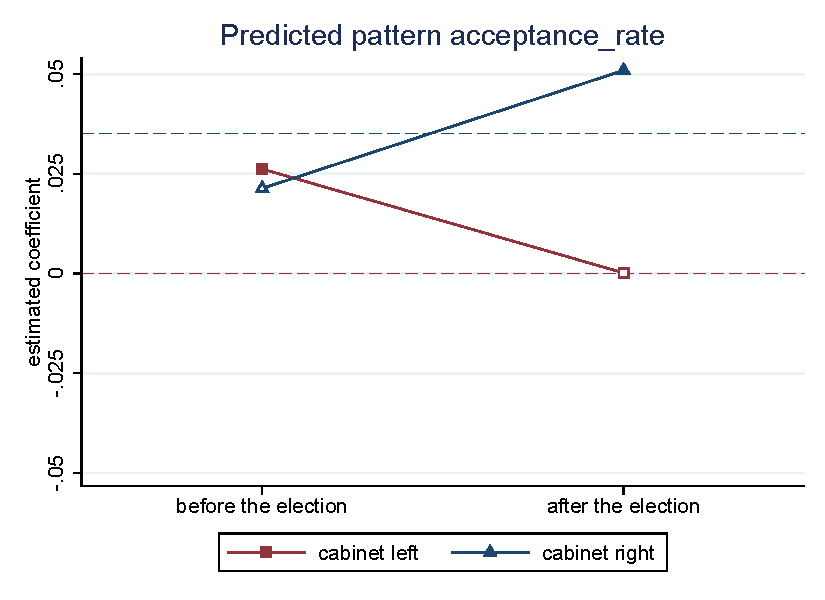
\includegraphics[width=1\textwidth]{figures_edited/acceptance_rate_graph1_R12.pdf}
	\caption{R12: Acceptance Rate: Predicted Pattern}
\end{figure}

\begin{table}[!ht]\centering
	\renewcommand{\arraystretch}{1.25}
	\def\sym#1{\ifmmode^{#1}\else\(^{#1}\)\fi}
	\caption{R12: Acceptance Rate: Predicted Pattern}
	\begin{tabular}{l*{2}{c}}
		\hline\hline
		                    &\multicolumn{1}{c}{(1)}&\multicolumn{1}{c}{(2)}\\
                    &\multicolumn{1}{c}{left}&\multicolumn{1}{c}{right}\\
\hline
before              &      0.0262\sym{**} &     -0.0138         \\
                    &   (0.00859)         &   (0.00754)         \\
after               &    0.000177         &      0.0158\sym{**} \\
                    &   (0.00552)         &   (0.00541)         \\
\hline
Observations        &       17193         &       17193         \\

		\hline\hline
		\multicolumn{3}{c}{\footnotesize Standard errors in parentheses} \\
		\multicolumn{3}{c}{\footnotesize (\sym{*} \(p<0.05\), \sym{**} \(p<0.01\), \sym{***} \(p<0.001\))}\\
	\end{tabular}
\end{table}

\clearpage
\textbf{R12: Split cabinet position at 5 to determine cabinet left-right dummies - Model 2}
\begin{figure}[!ht]
	\centering
	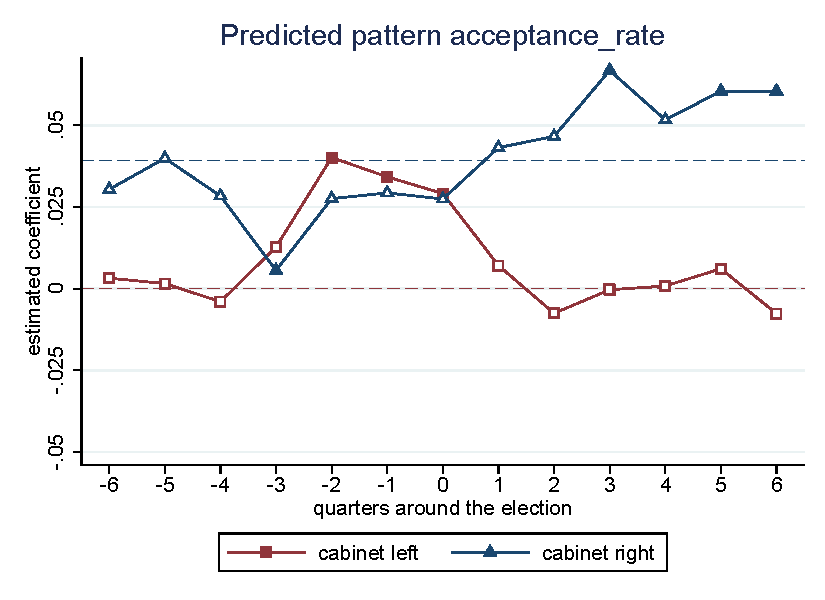
\includegraphics[width=0.7\textwidth]{figures_edited/acceptance_rate_graph2_R12.pdf}
	\caption{R12: Acceptance Rate: Predicted Pattern}
\end{figure}

\begin{table}[!ht]\centering
	\footnotesize
	\renewcommand{\arraystretch}{1.2}
	\def\sym#1{\ifmmode^{#1}\else\(^{#1}\)\fi}
	\caption{R12: Acceptance Rate: Predicted Pattern}
	\begin{tabular}{l*{2}{c}}
		\hline\hline
		                    &\multicolumn{1}{c}{(1)}&\multicolumn{1}{c}{(2)}\\
                    &\multicolumn{1}{c}{left}&\multicolumn{1}{c}{right}\\
\hline
 6 quarters before the election&      0.0103         &     -0.0116         \\
                    &    (0.0122)         &   (0.00685)         \\
 5 quarters before the election&     0.00882         &    -0.00627         \\
                    &    (0.0132)         &   (0.00872)         \\
 4 quarters before the election&     0.00309         &     -0.0170         \\
                    &    (0.0118)         &    (0.0115)         \\
 3 quarters before the election&      0.0143         &     -0.0350\sym{**} \\
                    &    (0.0142)         &    (0.0123)         \\
 2 quarters before the election&      0.0463\sym{***}&     -0.0155         \\
                    &   (0.00972)         &    (0.0107)         \\
 1 quarters before the election&      0.0417\sym{***}&    -0.00844         \\
                    &    (0.0123)         &    (0.0106)         \\
Quarter of the election&      0.0402\sym{**} &     -0.0143         \\
                    &    (0.0129)         &    (0.0121)         \\
 1 quarters after the election&     0.00799         &     0.00252         \\
                    &    (0.0104)         &    (0.0108)         \\
 2 quarters after the election&    -0.00638         &     0.00639         \\
                    &   (0.00874)         &   (0.00910)         \\
 3 quarters after the election&    -0.00138         &      0.0245\sym{**} \\
                    &   (0.00828)         &   (0.00914)         \\
 4 quarters after the election&     0.00895         &     0.00682         \\
                    &    (0.0103)         &   (0.00950)         \\
 5 quarters after the election&     0.00950         &      0.0202\sym{*}  \\
                    &    (0.0114)         &   (0.00808)         \\
 6 quarters after the election&    -0.00356         &      0.0193\sym{**} \\
                    &    (0.0110)         &   (0.00745)         \\
\hline
Observations        &       17193         &       17193         \\

		\hline\hline
		\multicolumn{3}{c}{\footnotesize Standard errors in parentheses} \\
		\multicolumn{3}{c}{\footnotesize (\sym{*} \(p<0.05\), \sym{**} \(p<0.01\), \sym{***} \(p<0.001\))} \\
	\end{tabular}
\end{table}



% ===============================================================================================================


\clearpage
\FloatBarrier
\subsubsection{Use only 5 quarters around the election}
\begin{table}[!ht]\centering
	\renewcommand{\arraystretch}{1.25}
	\small
	\def\sym#1{\ifmmode^{#1}\else\(^{#1}\)\fi}
	\caption{R13: Determinants of acceptance rate}
	\begin{tabular}{l*{3}{c}}
		\hline\hline
		                                        &\multicolumn{1}{c}{(1)}         &\multicolumn{1}{c}{(2)}         &\multicolumn{1}{c}{(3)}         \\
\hline
Political Terror Scale                  &    0.0167         &    0.0218\sym{*}  &                   \\
                                        & (0.00985)         &  (0.0102)         &                   \\
Civic Liberty (FHI)                     &    0.0405\sym{*}  &    0.0375         &                   \\
                                        &  (0.0191)         &  (0.0192)         &                   \\
Political Rights (FHI)                  &  -0.00991         &  -0.00813         &                   \\
                                        &  (0.0150)         &  (0.0161)         &                   \\
Quarterly civil war battle death (000s) &    0.0451\sym{***}&    0.0451\sym{***}&                   \\
                                        & (0.00430)         & (0.00474)         &                   \\
Log origin country real GDP per capita  &   -0.0165         &   -0.0200         &                   \\
                                        &  (0.0316)         &  (0.0366)         &                   \\
Log migrant stock in 2000/1             & -0.000751         &                   & -0.000256         \\
                                        & (0.00240)         &                   & (0.00245)         \\
Log distance from origin to destination &    0.0141         &                   &    0.0153         \\
                                        &  (0.0232)         &                   &  (0.0234)         \\
Log destination country real GDP per capita&    0.0652         &    0.0949         &    0.0713         \\
                                        &  (0.0684)         &  (0.0726)         &  (0.0660)         \\
Quarterly unemployment rate at destination&  -0.00111         &  -0.00111         &  -0.00133         \\
                                        & (0.00126)         & (0.00116)         & (0.00130)         \\
Log average past total asylum decisions per capita&    -159.3\sym{***}&    -168.3\sym{***}&    -158.4\sym{***}\\
                                        &   (36.29)         &   (37.56)         &   (37.98)         \\
Log average past dyadic asylum decisions per capita&     419.7\sym{*}  &     297.8         &     272.9         \\
                                        &   (195.5)         &   (227.8)         &   (208.6)         \\
Weighted cabinet position right         &    0.0297\sym{**} &    0.0319\sym{**} &    0.0290\sym{**} \\
                                        &  (0.0102)         &  (0.0102)         &  (0.0106)         \\
Cabinet position left * Before the election&    0.0130\sym{*}  &    0.0158\sym{*}  &    0.0125         \\
                                        & (0.00625)         & (0.00622)         & (0.00621)         \\
Cabinet position left * After the election&   0.00147         &   0.00101         &   0.00234         \\
                                        & (0.00488)         & (0.00502)         & (0.00523)         \\
Cabinet position right * Before the election&   -0.0140         &   -0.0153         &   -0.0129         \\
                                        & (0.00829)         & (0.00808)         & (0.00826)         \\
Cabinet position right * After the election&    0.0246\sym{***}&    0.0224\sym{***}&    0.0232\sym{***}\\
                                        & (0.00600)         & (0.00590)         & (0.00626)         \\
\hline
Observations                            &     17193         &     17193         &     17193         \\
Adjusted \(R^{2}\)                      &     0.156         &     0.105         &     0.104         \\
Fixed Effects                           &         O         &     D x O         &     O x T         \\
Destination dummies                     &       Yes         &        No         &       Yes         \\
Quarter-Year dummies                    &       Yes         &       Yes         &        No         \\

		\hline\hline
		\multicolumn{4}{l}{\footnotesize Standard errors in parentheses (\sym{*} \(p<0.05\), \sym{**} \(p<0.01\), \sym{***} \(p<0.001\))}\\
	\end{tabular}
\end{table}

\clearpage
\textbf{R13: Use only 5 quarters around the election - Model 1}
\begin{figure}[!ht]
	\centering
	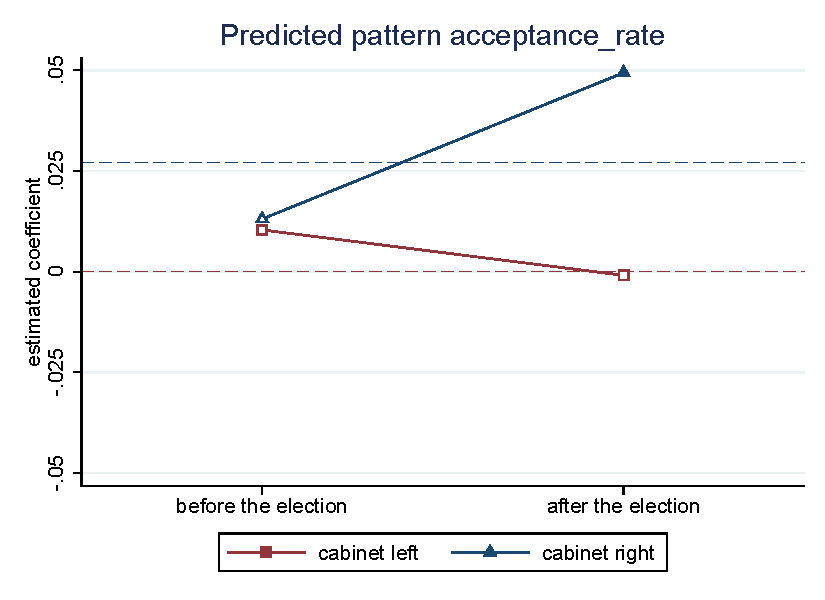
\includegraphics[width=1\textwidth]{figures_edited/acceptance_rate_graph1_R13.pdf}
	\caption{R13: Acceptance Rate: Predicted Pattern}
\end{figure}

\begin{table}[!ht]\centering
	\renewcommand{\arraystretch}{1.25}
	\def\sym#1{\ifmmode^{#1}\else\(^{#1}\)\fi}
	\caption{R13: Acceptance Rate: Predicted Pattern}
	\begin{tabular}{l*{2}{c}}
		\hline\hline
		                    &\multicolumn{1}{c}{(1)}&\multicolumn{1}{c}{(2)}\\
                    &\multicolumn{1}{c}{left}&\multicolumn{1}{c}{right}\\
\hline
before              &      0.0158\sym{*}  &     -0.0153         \\
                    &   (0.00622)         &   (0.00808)         \\
after               &     0.00101         &      0.0224\sym{***}\\
                    &   (0.00502)         &   (0.00590)         \\
\hline
Observations        &       17193         &       17193         \\

		\hline\hline
		\multicolumn{3}{c}{\footnotesize Standard errors in parentheses} \\
		\multicolumn{3}{c}{\footnotesize (\sym{*} \(p<0.05\), \sym{**} \(p<0.01\), \sym{***} \(p<0.001\))}\\
	\end{tabular}
\end{table}

\clearpage
\textbf{R13: Use only 5 quarters around the election - Model 2}
\begin{figure}[!ht]
	\centering
	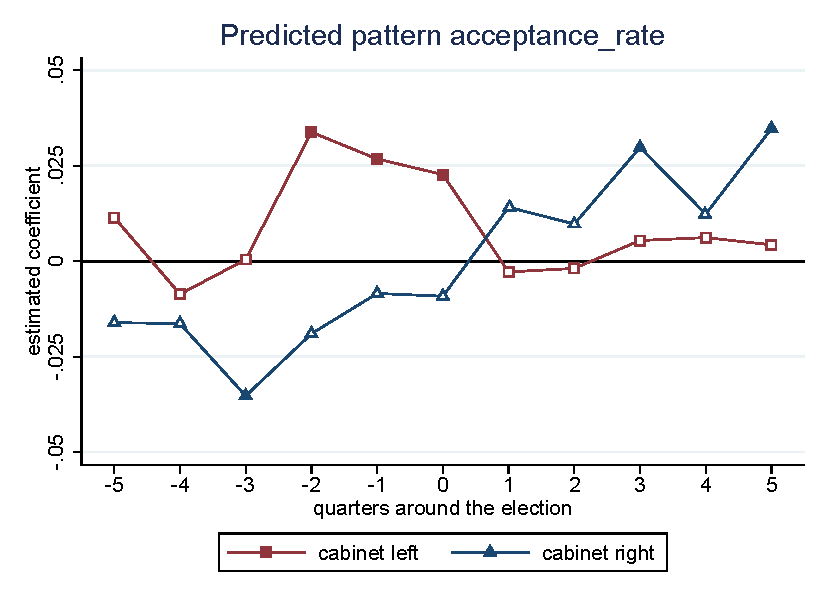
\includegraphics[width=0.7\textwidth]{figures_edited/acceptance_rate_graph2_R13.pdf}
	\caption{R13: Acceptance Rate: Predicted Pattern}
\end{figure}

\begin{table}[!ht]\centering
	\footnotesize
	\renewcommand{\arraystretch}{1.2}
	\def\sym#1{\ifmmode^{#1}\else\(^{#1}\)\fi}
	\caption{R13: Acceptance Rate: Predicted Pattern}
	\begin{tabular}{l*{2}{c}}
		\hline\hline
		                    &\multicolumn{1}{c}{(1)}&\multicolumn{1}{c}{(2)}\\
                    &\multicolumn{1}{c}{left}&\multicolumn{1}{c}{right}\\
\hline
 5 quarters before the election&      0.0115         &     -0.0161         \\
                    &    (0.0102)         &   (0.00971)         \\
 4 quarters before the election&    -0.00862         &     -0.0163         \\
                    &   (0.00887)         &    (0.0103)         \\
 3 quarters before the election&    0.000458         &     -0.0353\sym{**} \\
                    &    (0.0130)         &    (0.0115)         \\
 2 quarters before the election&      0.0338\sym{***}&     -0.0190         \\
                    &   (0.00864)         &    (0.0107)         \\
 1 quarters before the election&      0.0268\sym{**} &    -0.00844         \\
                    &   (0.00872)         &    (0.0104)         \\
Quarter of the election&      0.0227\sym{*}  &    -0.00915         \\
                    &   (0.00928)         &    (0.0137)         \\
 1 quarters after the election&    -0.00280         &      0.0141         \\
                    &   (0.00692)         &    (0.0120)         \\
 2 quarters after the election&    -0.00188         &     0.00975         \\
                    &   (0.00770)         &   (0.00873)         \\
 3 quarters after the election&     0.00543         &      0.0298\sym{**} \\
                    &   (0.00725)         &    (0.0104)         \\
 4 quarters after the election&     0.00619         &      0.0123         \\
                    &   (0.00751)         &   (0.00805)         \\
 5 quarters after the election&     0.00430         &      0.0347\sym{***}\\
                    &   (0.00742)         &    (0.0104)         \\
\hline
Observations        &       17193         &       17193         \\

		\hline\hline
		\multicolumn{3}{c}{\footnotesize Standard errors in parentheses} \\
		\multicolumn{3}{c}{\footnotesize (\sym{*} \(p<0.05\), \sym{**} \(p<0.01\), \sym{***} \(p<0.001\))} \\
	\end{tabular}
\end{table}



% ===============================================================================================================


\clearpage
\FloatBarrier
\subsubsection{Use only 4 quarters around the election}
\begin{table}[!ht]\centering
	\renewcommand{\arraystretch}{1.25}
	\small
	\def\sym#1{\ifmmode^{#1}\else\(^{#1}\)\fi}
	\caption{R14: Determinants of acceptance rate}
	\begin{tabular}{l*{3}{c}}
		\hline\hline
		                                        &\multicolumn{1}{c}{(1)}         &\multicolumn{1}{c}{(2)}         &\multicolumn{1}{c}{(3)}         \\
\hline
Political Terror Scale                  &    0.0167         &    0.0218\sym{*}  &                   \\
                                        & (0.00987)         &  (0.0103)         &                   \\
Civic Liberty (FHI)                     &    0.0405\sym{*}  &    0.0376         &                   \\
                                        &  (0.0191)         &  (0.0192)         &                   \\
Political Rights (FHI)                  &  -0.00995         &  -0.00818         &                   \\
                                        &  (0.0150)         &  (0.0161)         &                   \\
Quarterly civil war battle death (000s) &    0.0451\sym{***}&    0.0451\sym{***}&                   \\
                                        & (0.00431)         & (0.00475)         &                   \\
Log origin country real GDP per capita  &   -0.0166         &   -0.0201         &                   \\
                                        &  (0.0317)         &  (0.0367)         &                   \\
Log migrant stock in 2000/1             & -0.000749         &                   & -0.000255         \\
                                        & (0.00241)         &                   & (0.00245)         \\
Log distance from origin to destination &    0.0143         &                   &    0.0154         \\
                                        &  (0.0231)         &                   &  (0.0234)         \\
Log destination country real GDP per capita&    0.0678         &    0.0972         &    0.0741         \\
                                        &  (0.0684)         &  (0.0725)         &  (0.0660)         \\
Quarterly unemployment rate at destination& -0.000985         &  -0.00100         &  -0.00121         \\
                                        & (0.00126)         & (0.00115)         & (0.00130)         \\
Log average past total asylum decisions per capita&    -161.0\sym{***}&    -170.0\sym{***}&    -160.1\sym{***}\\
                                        &   (36.70)         &   (37.87)         &   (38.39)         \\
Log average past dyadic asylum decisions per capita&     421.2\sym{*}  &     299.7         &     274.9         \\
                                        &   (195.5)         &   (226.4)         &   (208.8)         \\
Weighted cabinet position right         &    0.0334\sym{**} &    0.0350\sym{**} &    0.0329\sym{**} \\
                                        &  (0.0107)         &  (0.0106)         &  (0.0109)         \\
Cabinet position left * Before the election&    0.0200\sym{**} &    0.0215\sym{**} &    0.0204\sym{**} \\
                                        & (0.00623)         & (0.00636)         & (0.00625)         \\
Cabinet position left * After the election&   0.00222         &   0.00135         &   0.00331         \\
                                        & (0.00448)         & (0.00467)         & (0.00478)         \\
Cabinet position right * Before the election&   -0.0154         &   -0.0178\sym{*}  &   -0.0145         \\
                                        & (0.00843)         & (0.00837)         & (0.00848)         \\
Cabinet position right * After the election&    0.0177\sym{**} &    0.0157\sym{**} &    0.0164\sym{**} \\
                                        & (0.00578)         & (0.00574)         & (0.00609)         \\
\hline
Observations                            &     17193         &     17193         &     17193         \\
Adjusted \(R^{2}\)                      &     0.155         &     0.105         &     0.103         \\
Fixed Effects                           &         O         &     D x O         &     O x T         \\
Destination dummies                     &       Yes         &        No         &       Yes         \\
Quarter-Year dummies                    &       Yes         &       Yes         &        No         \\

		\hline\hline
		\multicolumn{4}{l}{\footnotesize Standard errors in parentheses (\sym{*} \(p<0.05\), \sym{**} \(p<0.01\), \sym{***} \(p<0.001\))}\\
	\end{tabular}
\end{table}

\clearpage
\textbf{R14: Use only 4 quarters around the election - Model 1}
\begin{figure}[!ht]
	\centering
	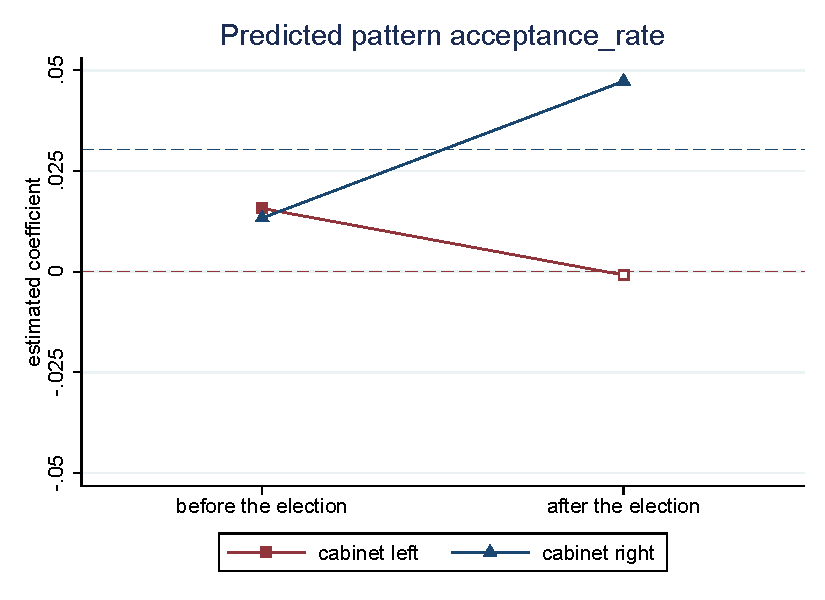
\includegraphics[width=1\textwidth]{figures_edited/acceptance_rate_graph1_R14.pdf}
	\caption{R14: Acceptance Rate: Predicted Pattern}
\end{figure}

\begin{table}[!ht]\centering
	\renewcommand{\arraystretch}{1.25}
	\def\sym#1{\ifmmode^{#1}\else\(^{#1}\)\fi}
	\caption{R14: Acceptance Rate: Predicted Pattern}
	\begin{tabular}{l*{2}{c}}
		\hline\hline
		                    &\multicolumn{1}{c}{(1)}&\multicolumn{1}{c}{(2)}\\
                    &\multicolumn{1}{c}{left}&\multicolumn{1}{c}{right}\\
\hline
before              &      0.0215\sym{***}&     -0.0178\sym{*}  \\
                    &   (0.00636)         &   (0.00837)         \\
after               &     0.00135         &      0.0157\sym{**} \\
                    &   (0.00467)         &   (0.00574)         \\
\hline
Observations        &       17193         &       17193         \\

		\hline\hline
		\multicolumn{3}{c}{\footnotesize Standard errors in parentheses} \\
		\multicolumn{3}{c}{\footnotesize (\sym{*} \(p<0.05\), \sym{**} \(p<0.01\), \sym{***} \(p<0.001\))}\\
	\end{tabular}
\end{table}

\clearpage
\textbf{R14: Use only 4 quarters around the election - Model 2}
\begin{figure}[!ht]
	\centering
	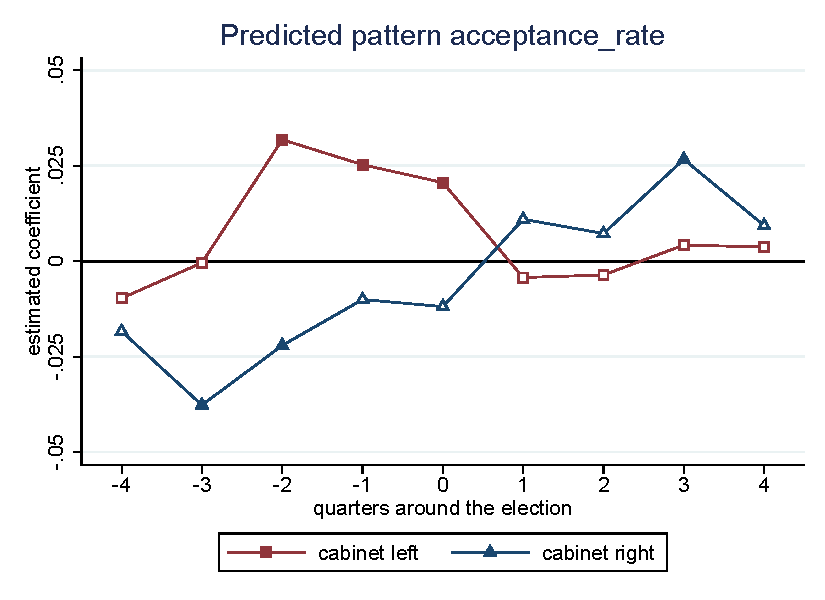
\includegraphics[width=0.7\textwidth]{figures_edited/acceptance_rate_graph2_R14.pdf}
	\caption{R14: Acceptance Rate: Predicted Pattern}
\end{figure}

\begin{table}[!ht]\centering
	\footnotesize
	\renewcommand{\arraystretch}{1.2}
	\def\sym#1{\ifmmode^{#1}\else\(^{#1}\)\fi}
	\caption{R14: Acceptance Rate: Predicted Pattern}
	\begin{tabular}{l*{2}{c}}
		\hline\hline
		                    &\multicolumn{1}{c}{(1)}&\multicolumn{1}{c}{(2)}\\
                    &\multicolumn{1}{c}{left}&\multicolumn{1}{c}{right}\\
\hline
 4 quarters before the election&    -0.00969         &     -0.0183         \\
                    &   (0.00966)         &   (0.00978)         \\
 3 quarters before the election&   -0.000403         &     -0.0377\sym{***}\\
                    &    (0.0132)         &    (0.0112)         \\
 2 quarters before the election&      0.0318\sym{***}&     -0.0221\sym{*}  \\
                    &   (0.00866)         &    (0.0102)         \\
 1 quarters before the election&      0.0253\sym{**} &     -0.0100         \\
                    &   (0.00865)         &    (0.0101)         \\
Quarter of the election&      0.0206\sym{*}  &     -0.0119         \\
                    &   (0.00951)         &    (0.0135)         \\
 1 quarters after the election&    -0.00426         &      0.0110         \\
                    &   (0.00696)         &    (0.0115)         \\
 2 quarters after the election&    -0.00360         &     0.00726         \\
                    &   (0.00799)         &   (0.00782)         \\
 3 quarters after the election&     0.00424         &      0.0267\sym{**} \\
                    &   (0.00722)         &    (0.0101)         \\
 4 quarters after the election&     0.00373         &     0.00937         \\
                    &   (0.00714)         &   (0.00750)         \\
\hline
Observations        &       17193         &       17193         \\

		\hline\hline
		\multicolumn{3}{c}{\footnotesize Standard errors in parentheses} \\
		\multicolumn{3}{c}{\footnotesize (\sym{*} \(p<0.05\), \sym{**} \(p<0.01\), \sym{***} \(p<0.001\))} \\
	\end{tabular}
\end{table}



% ===============================================================================================================


\clearpage
\FloatBarrier
\subsubsection{Impute total decisions from all positive and rejected decisions}
\begin{table}[!ht]\centering
	\renewcommand{\arraystretch}{1.25}
	\small
	\def\sym#1{\ifmmode^{#1}\else\(^{#1}\)\fi}
	\caption{R15: Determinants of acceptance rate}
	\begin{tabular}{l*{3}{c}}
		\hline\hline
		                                        &\multicolumn{1}{c}{(1)}         &\multicolumn{1}{c}{(2)}         &\multicolumn{1}{c}{(3)}         \\
\hline
Political Terror Scale                  &    0.0196         &    0.0232\sym{*}  &                   \\
                                        &  (0.0107)         &  (0.0112)         &                   \\
Civic Liberty (FHI)                     &    0.0384         &    0.0376         &                   \\
                                        &  (0.0192)         &  (0.0196)         &                   \\
Political Rights (FHI)                  &  -0.00938         &  -0.00851         &                   \\
                                        &  (0.0155)         &  (0.0166)         &                   \\
Quarterly civil war battle death (000s) &    0.0444\sym{***}&    0.0449\sym{***}&                   \\
                                        & (0.00515)         & (0.00562)         &                   \\
Log origin country real GDP per capita  &   -0.0283         &   -0.0319         &                   \\
                                        &  (0.0310)         &  (0.0359)         &                   \\
Log migrant stock in 2000/1             &   0.00103         &                   &   0.00152         \\
                                        & (0.00223)         &                   & (0.00228)         \\
Log distance from origin to destination &   0.00612         &                   &   0.00797         \\
                                        &  (0.0215)         &                   &  (0.0222)         \\
Log destination country real GDP per capita&    0.0513         &    0.0778         &    0.0613         \\
                                        &  (0.0753)         &  (0.0769)         &  (0.0750)         \\
Quarterly unemployment rate at destination&  -0.00165         &  -0.00162         &  -0.00201         \\
                                        & (0.00132)         & (0.00124)         & (0.00136)         \\
Log average past total asylum decisions per capita&    -115.6\sym{**} &    -117.0\sym{**} &    -110.5\sym{**} \\
                                        &   (33.77)         &   (35.38)         &   (35.72)         \\
Log average past dyadic asylum decisions per capita&     468.8\sym{*}  &     272.9         &     285.0         \\
                                        &   (201.8)         &   (242.9)         &   (221.6)         \\
Weighted cabinet position right         &    0.0174         &    0.0198         &    0.0158         \\
                                        & (0.00972)         & (0.00989)         &  (0.0100)         \\
Cabinet position left * Before the election&   0.00937         &    0.0123         &   0.00959         \\
                                        & (0.00617)         & (0.00626)         & (0.00636)         \\
Cabinet position left * After the election&  -0.00171         &  -0.00196         & -0.000650         \\
                                        & (0.00540)         & (0.00541)         & (0.00552)         \\
Cabinet position right * Before the election&  -0.00986         &   -0.0104         &  -0.00771         \\
                                        & (0.00784)         & (0.00771)         & (0.00792)         \\
Cabinet position right * After the election&    0.0258\sym{***}&    0.0236\sym{***}&    0.0257\sym{***}\\
                                        & (0.00618)         & (0.00583)         & (0.00626)         \\
\hline
Observations                            &     17777         &     17777         &     17777         \\
Adjusted \(R^{2}\)                      &     0.145         &     0.102         &     0.087         \\
Fixed Effects                           &         O         &     D x O         &     O x T         \\
Destination dummies                     &       Yes         &        No         &       Yes         \\
Quarter-Year dummies                    &       Yes         &       Yes         &        No         \\

		\hline\hline
		\multicolumn{4}{l}{\footnotesize Standard errors in parentheses (\sym{*} \(p<0.05\), \sym{**} \(p<0.01\), \sym{***} \(p<0.001\))}\\
	\end{tabular}
\end{table}

\clearpage
\textbf{R15: Impute total decisions from all positive and rejected decisions - Model 1}
\begin{figure}[!ht]
	\centering
	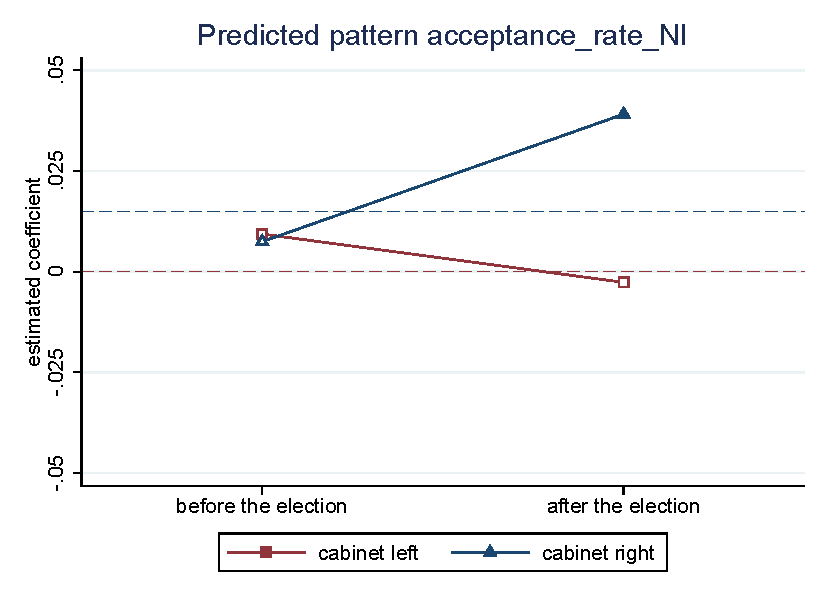
\includegraphics[width=1\textwidth]{figures_edited/acceptance_rate_NI_graph1_R15.pdf}
	\caption{R15: Acceptance Rate: Predicted Pattern}
\end{figure}

\begin{table}[!ht]\centering
	\renewcommand{\arraystretch}{1.25}
	\def\sym#1{\ifmmode^{#1}\else\(^{#1}\)\fi}
	\caption{R15: Acceptance Rate: Predicted Pattern}
	\begin{tabular}{l*{2}{c}}
		\hline\hline
		                    &\multicolumn{1}{c}{(1)}&\multicolumn{1}{c}{(2)}\\
                    &\multicolumn{1}{c}{left}&\multicolumn{1}{c}{right}\\
\hline
before              &      0.0123\sym{*}  &     -0.0104         \\
                    &   (0.00626)         &   (0.00771)         \\
after               &    -0.00196         &      0.0236\sym{***}\\
                    &   (0.00541)         &   (0.00583)         \\
\hline
Observations        &       17777         &       17777         \\

		\hline\hline
		\multicolumn{3}{c}{\footnotesize Standard errors in parentheses} \\
		\multicolumn{3}{c}{\footnotesize (\sym{*} \(p<0.05\), \sym{**} \(p<0.01\), \sym{***} \(p<0.001\))}\\
	\end{tabular}
\end{table}

\clearpage
\textbf{R15: Impute total decisions from all positive and rejected decisions - Model 2}
\begin{figure}[!ht]
	\centering
	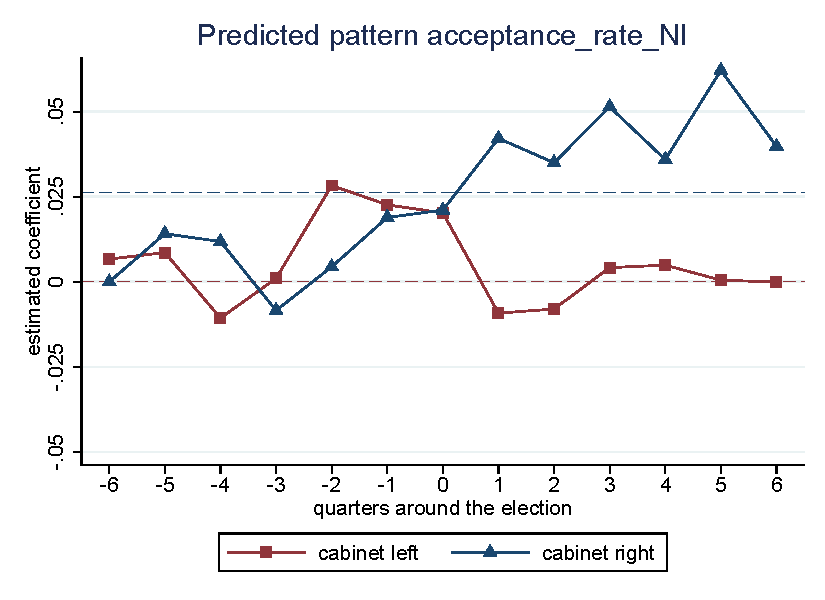
\includegraphics[width=0.7\textwidth]{figures_edited/acceptance_rate_NI_graph2_R15.pdf}
	\caption{R15: Acceptance Rate: Predicted Pattern}
\end{figure}

\begin{table}[!ht]\centering
	\footnotesize
	\renewcommand{\arraystretch}{1.2}
	\def\sym#1{\ifmmode^{#1}\else\(^{#1}\)\fi}
	\caption{R15: Acceptance Rate: Predicted Pattern}
	\begin{tabular}{l*{2}{c}}
		\hline\hline
		                    &\multicolumn{1}{c}{(1)}&\multicolumn{1}{c}{(2)}\\
                    &\multicolumn{1}{c}{left}&\multicolumn{1}{c}{right}\\
\hline
 6 quarters before the election&     0.00669         &     -0.0262\sym{***}\\
                    &    (0.0106)         &   (0.00704)         \\
 5 quarters before the election&     0.00862         &     -0.0121         \\
                    &   (0.00949)         &   (0.00823)         \\
 4 quarters before the election&     -0.0106         &     -0.0143         \\
                    &    (0.0108)         &    (0.0110)         \\
 3 quarters before the election&     0.00102         &     -0.0346\sym{**} \\
                    &    (0.0131)         &    (0.0117)         \\
 2 quarters before the election&      0.0283\sym{***}&     -0.0218\sym{*}  \\
                    &   (0.00859)         &   (0.00980)         \\
 1 quarters before the election&      0.0226\sym{*}  &    -0.00727         \\
                    &   (0.00974)         &    (0.0118)         \\
Quarter of the election&      0.0202         &    -0.00511         \\
                    &    (0.0113)         &    (0.0144)         \\
 1 quarters after the election&    -0.00917         &      0.0160         \\
                    &   (0.00762)         &    (0.0112)         \\
 2 quarters after the election&    -0.00797         &     0.00879         \\
                    &   (0.00973)         &   (0.00946)         \\
 3 quarters after the election&     0.00420         &      0.0252\sym{*}  \\
                    &   (0.00814)         &    (0.0112)         \\
 4 quarters after the election&     0.00491         &     0.00974         \\
                    &   (0.00888)         &   (0.00756)         \\
 5 quarters after the election&    0.000508         &      0.0359\sym{**} \\
                    &   (0.00942)         &    (0.0111)         \\
 6 quarters after the election&  -0.0000449         &      0.0136         \\
                    &   (0.00939)         &   (0.00770)         \\
\hline
Observations        &       17777         &       17777         \\

		\hline\hline
		\multicolumn{3}{c}{\footnotesize Standard errors in parentheses} \\
		\multicolumn{3}{c}{\footnotesize (\sym{*} \(p<0.05\), \sym{**} \(p<0.01\), \sym{***} \(p<0.001\))} \\
	\end{tabular}
\end{table}




% ===============================================================================================================


\clearpage
\FloatBarrier
\subsubsection{Include refugee crisis 2015 and 2016}
\begin{table}[!ht]\centering
	\renewcommand{\arraystretch}{1.25}
	\small
	\def\sym#1{\ifmmode^{#1}\else\(^{#1}\)\fi}
	\caption{R16: Determinants of acceptance rate}
	\begin{tabular}{l*{3}{c}}
		\hline\hline
		                                        &\multicolumn{1}{c}{(1)}         &\multicolumn{1}{c}{(2)}         &\multicolumn{1}{c}{(3)}         \\
\hline
Political Terror Scale                  &    0.0244         &    0.0287\sym{*}  &                   \\
                                        &  (0.0132)         &  (0.0135)         &                   \\
Civic Liberty (FHI)                     &    0.0328         &    0.0297         &                   \\
                                        &  (0.0197)         &  (0.0198)         &                   \\
Political Rights (FHI)                  &   -0.0101         &  -0.00867         &                   \\
                                        &  (0.0155)         &  (0.0163)         &                   \\
Quarterly civil war battle death (000s) &    0.0458\sym{***}&    0.0447\sym{***}&                   \\
                                        & (0.00509)         & (0.00515)         &                   \\
Log origin country real GDP per capita  &   -0.0443         &   -0.0454         &                   \\
                                        &  (0.0355)         &  (0.0383)         &                   \\
Log migrant stock in 2000/1             &  -0.00437         &                   &  -0.00360         \\
                                        & (0.00247)         &                   & (0.00250)         \\
Log distance from origin to destination &   0.00418         &                   &   0.00634         \\
                                        &  (0.0258)         &                   &  (0.0258)         \\
Log destination country real GDP per capita&    0.0910         &    0.0895         &    0.0878         \\
                                        &  (0.0566)         &  (0.0590)         &  (0.0560)         \\
Quarterly unemployment rate at destination&   0.00143         &   0.00110         &   0.00101         \\
                                        & (0.00134)         & (0.00125)         & (0.00135)         \\
Log average past total asylum decisions per capita&    -63.78\sym{**} &    -62.69\sym{**} &    -58.22\sym{**} \\
                                        &   (19.64)         &   (19.89)         &   (17.05)         \\
Log average past dyadic asylum decisions per capita&     436.6\sym{*}  &     388.8\sym{*}  &     159.4         \\
                                        &   (165.7)         &   (149.0)         &   (129.1)         \\
Weighted cabinet position right         &    0.0136         &    0.0168         &    0.0108         \\
                                        &  (0.0115)         &  (0.0118)         &  (0.0119)         \\
Cabinet position left * Before the election&    0.0145\sym{*}  &    0.0179\sym{**} &    0.0129\sym{*}  \\
                                        & (0.00608)         & (0.00616)         & (0.00628)         \\
Cabinet position left * After the election& -0.000775         &-0.0000405         &  -0.00164         \\
                                        & (0.00523)         & (0.00554)         & (0.00563)         \\
Cabinet position right * Before the election&  -0.00640         &  -0.00885         &  -0.00496         \\
                                        & (0.00822)         & (0.00854)         & (0.00843)         \\
Cabinet position right * After the election&    0.0172\sym{**} &    0.0169\sym{**} &    0.0156\sym{**} \\
                                        & (0.00494)         & (0.00484)         & (0.00547)         \\
\hline
Observations                            &     18410         &     18410         &     18410         \\
Adjusted \(R^{2}\)                      &     0.166         &     0.114         &     0.097         \\
Fixed Effects                           &         O         &     D x O         &     O x T         \\
Destination dummies                     &       Yes         &        No         &       Yes         \\
Quarter-Year dummies                    &       Yes         &       Yes         &        No         \\

		\hline\hline
		\multicolumn{4}{l}{\footnotesize Standard errors in parentheses (\sym{*} \(p<0.05\), \sym{**} \(p<0.01\), \sym{***} \(p<0.001\))}\\
	\end{tabular}
\end{table}

\clearpage
\textbf{R16: Include refugee crisis 2015 and 2016 - Model 1}
\begin{figure}[!ht]
	\centering
	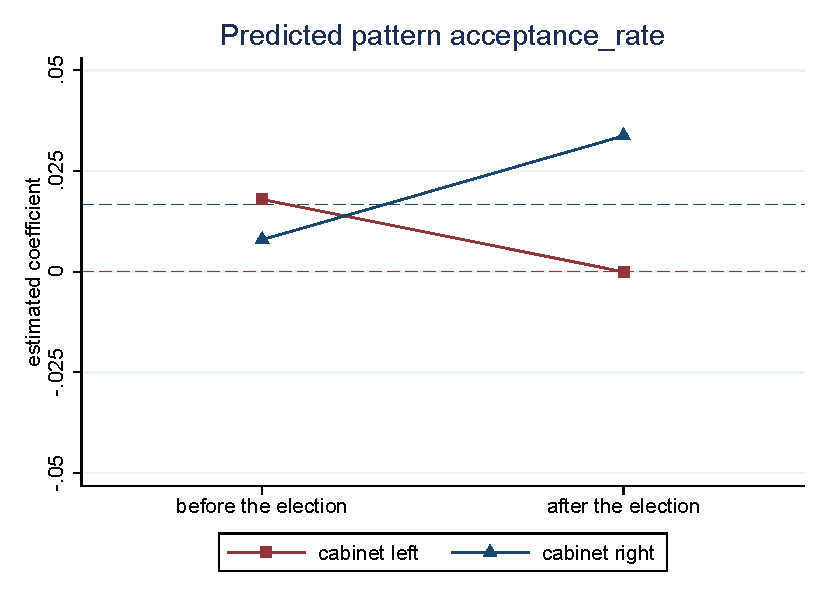
\includegraphics[width=1\textwidth]{figures_edited/acceptance_rate_graph1_R16.pdf}
	\caption{R16: Acceptance Rate: Predicted Pattern}
\end{figure}

\begin{table}[!ht]\centering
	\renewcommand{\arraystretch}{1.25}
	\def\sym#1{\ifmmode^{#1}\else\(^{#1}\)\fi}
	\caption{R16: Acceptance Rate: Predicted Pattern}
	\begin{tabular}{l*{2}{c}}
		\hline\hline
		                    &\multicolumn{1}{c}{(1)}&\multicolumn{1}{c}{(2)}\\
                    &\multicolumn{1}{c}{left}&\multicolumn{1}{c}{right}\\
\hline
before              &      0.0179\sym{**} &    -0.00885         \\
                    &   (0.00616)         &   (0.00854)         \\
after               &  -0.0000405         &      0.0169\sym{***}\\
                    &   (0.00554)         &   (0.00484)         \\
\hline
Observations        &       18410         &       18410         \\

		\hline\hline
		\multicolumn{3}{c}{\footnotesize Standard errors in parentheses} \\
		\multicolumn{3}{c}{\footnotesize (\sym{*} \(p<0.05\), \sym{**} \(p<0.01\), \sym{***} \(p<0.001\))}\\
	\end{tabular}
\end{table}

\clearpage
\textbf{R16: Include refugee crisis 2015 and 2016 - Model 2}
\begin{figure}[!ht]
	\centering
	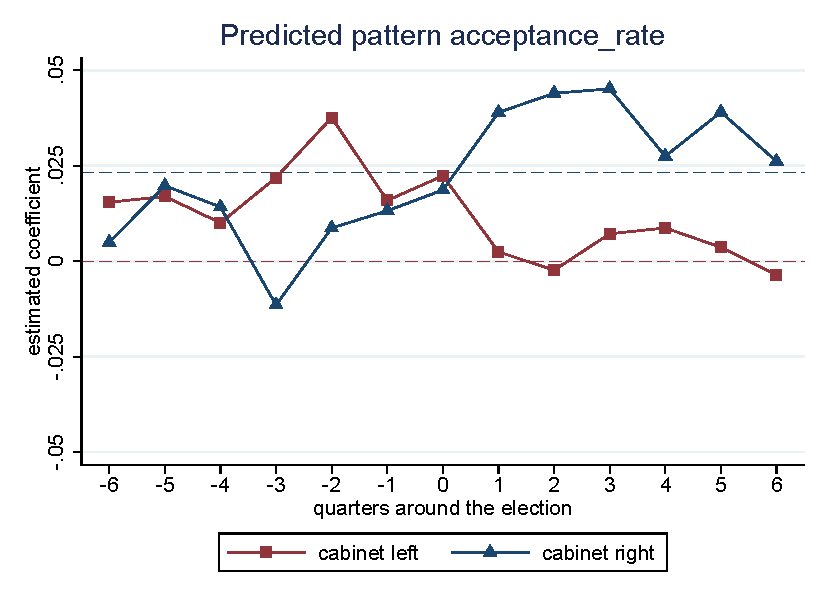
\includegraphics[width=0.7\textwidth]{figures_edited/acceptance_rate_graph2_R16.pdf}
	\caption{R16: Acceptance Rate: Predicted Pattern}
\end{figure}

\begin{table}[!ht]\centering
	\footnotesize
	\renewcommand{\arraystretch}{1.2}
	\def\sym#1{\ifmmode^{#1}\else\(^{#1}\)\fi}
	\caption{R16: Acceptance Rate: Predicted Pattern}
	\begin{tabular}{l*{2}{c}}
		\hline\hline
		                    &\multicolumn{1}{c}{(1)}&\multicolumn{1}{c}{(2)}\\
                    &\multicolumn{1}{c}{left}&\multicolumn{1}{c}{right}\\
\hline
 6 quarters before the election&      0.0154         &     -0.0184\sym{*}  \\
                    &    (0.0103)         &   (0.00792)         \\
 5 quarters before the election&      0.0170         &    -0.00352         \\
                    &   (0.00907)         &   (0.00946)         \\
 4 quarters before the election&      0.0100         &    -0.00908         \\
                    &   (0.00808)         &    (0.0110)         \\
 3 quarters before the election&      0.0219         &     -0.0348\sym{**} \\
                    &    (0.0114)         &    (0.0123)         \\
 2 quarters before the election&      0.0376\sym{***}&     -0.0146         \\
                    &   (0.00915)         &    (0.0107)         \\
 1 quarters before the election&      0.0159         &     -0.0101         \\
                    &   (0.00949)         &    (0.0117)         \\
Quarter of the election&      0.0224\sym{*}  &    -0.00462         \\
                    &   (0.00913)         &    (0.0150)         \\
 1 quarters after the election&     0.00247         &      0.0157         \\
                    &   (0.00736)         &    (0.0100)         \\
 2 quarters after the election&    -0.00236         &      0.0207         \\
                    &   (0.00939)         &    (0.0107)         \\
 3 quarters after the election&     0.00719         &      0.0219\sym{*}  \\
                    &   (0.00794)         &    (0.0101)         \\
 4 quarters after the election&     0.00873         &     0.00421         \\
                    &   (0.00804)         &   (0.00754)         \\
 5 quarters after the election&     0.00366         &      0.0158         \\
                    &   (0.00892)         &   (0.00896)         \\
 6 quarters after the election&    -0.00356         &     0.00288         \\
                    &   (0.00950)         &   (0.00745)         \\
\hline
Observations        &       18410         &       18410         \\

		\hline\hline
		\multicolumn{3}{c}{\footnotesize Standard errors in parentheses} \\
		\multicolumn{3}{c}{\footnotesize (\sym{*} \(p<0.05\), \sym{**} \(p<0.01\), \sym{***} \(p<0.001\))} \\
	\end{tabular}
\end{table}




% ===============================================================================================================


\clearpage
\FloatBarrier
\subsubsection{Use all destination countries with a maximum of two years missing decision data}
\begin{table}[!ht]\centering
	\renewcommand{\arraystretch}{1.25}
	\small
	\def\sym#1{\ifmmode^{#1}\else\(^{#1}\)\fi}
	\caption{R17: Determinants of acceptance rate}
	\begin{tabular}{l*{3}{c}}
		\hline\hline
		                                        &\multicolumn{1}{c}{(1)}         &\multicolumn{1}{c}{(2)}         &\multicolumn{1}{c}{(3)}         \\
\hline
Political Terror Scale                  &    0.0175         &    0.0211\sym{*}  &                   \\
                                        & (0.00872)         & (0.00921)         &                   \\
Civic Liberty (FHI)                     &    0.0413\sym{*}  &    0.0384\sym{*}  &                   \\
                                        &  (0.0169)         &  (0.0171)         &                   \\
Political Rights (FHI)                  &   -0.0106         &  -0.00845         &                   \\
                                        &  (0.0122)         &  (0.0133)         &                   \\
Quarterly civil war battle death (000s) &    0.0461\sym{***}&    0.0465\sym{***}&                   \\
                                        & (0.00369)         & (0.00389)         &                   \\
Log origin country real GDP per capita  &   -0.0147         &   -0.0176         &                   \\
                                        &  (0.0257)         &  (0.0300)         &                   \\
Log migrant stock in 2000/1             &  -0.00124         &                   & -0.000837         \\
                                        & (0.00237)         &                   & (0.00240)         \\
Log distance from origin to destination &   0.00851         &                   &   0.00923         \\
                                        &  (0.0226)         &                   &  (0.0228)         \\
Log destination country real GDP per capita&    -0.187         &    -0.172         &    -0.197         \\
                                        &   (0.103)         &   (0.107)         &   (0.108)         \\
Quarterly unemployment rate at destination&  -0.00499\sym{*}  &  -0.00468\sym{*}  &  -0.00548\sym{**} \\
                                        & (0.00188)         & (0.00180)         & (0.00192)         \\
Log average past total asylum decisions per capita&    -175.8\sym{***}&    -156.6\sym{***}&    -184.9\sym{***}\\
                                        &   (29.94)         &   (32.19)         &   (32.67)         \\
Log average past dyadic asylum decisions per capita&     490.5\sym{***}&     182.0         &     392.8\sym{*}  \\
                                        &   (128.5)         &   (134.4)         &   (156.6)         \\
Weighted cabinet position right         &    0.0198         &    0.0255\sym{*}  &    0.0178         \\
                                        &  (0.0103)         &  (0.0106)         &  (0.0106)         \\
Cabinet position left * Before the election&   0.00840         &    0.0137\sym{*}  &   0.00787         \\
                                        & (0.00600)         & (0.00571)         & (0.00599)         \\
Cabinet position left * After the election&  -0.00378         &  -0.00229         &  -0.00358         \\
                                        & (0.00590)         & (0.00611)         & (0.00593)         \\
Cabinet position right * Before the election&  -0.00899         &   -0.0101         &  -0.00786         \\
                                        & (0.00722)         & (0.00720)         & (0.00748)         \\
Cabinet position right * After the election&    0.0283\sym{***}&    0.0267\sym{***}&    0.0279\sym{***}\\
                                        & (0.00618)         & (0.00578)         & (0.00632)         \\
\hline
Observations                            &     18331         &     18331         &     18331         \\
Adjusted \(R^{2}\)                      &     0.164         &     0.097         &     0.117         \\
Fixed Effects                           &         O         &     D x O         &     O x T         \\
Destination dummies                     &       Yes         &        No         &       Yes         \\
Quarter-Year dummies                    &       Yes         &       Yes         &        No         \\

		\hline\hline
		\multicolumn{4}{l}{\footnotesize Standard errors in parentheses (\sym{*} \(p<0.05\), \sym{**} \(p<0.01\), \sym{***} \(p<0.001\))}\\
	\end{tabular}
\end{table}

\clearpage
\textbf{R17: Use all destination countries with a maximum of two years missing decision data - Model 1}
\begin{figure}[!ht]
	\centering
	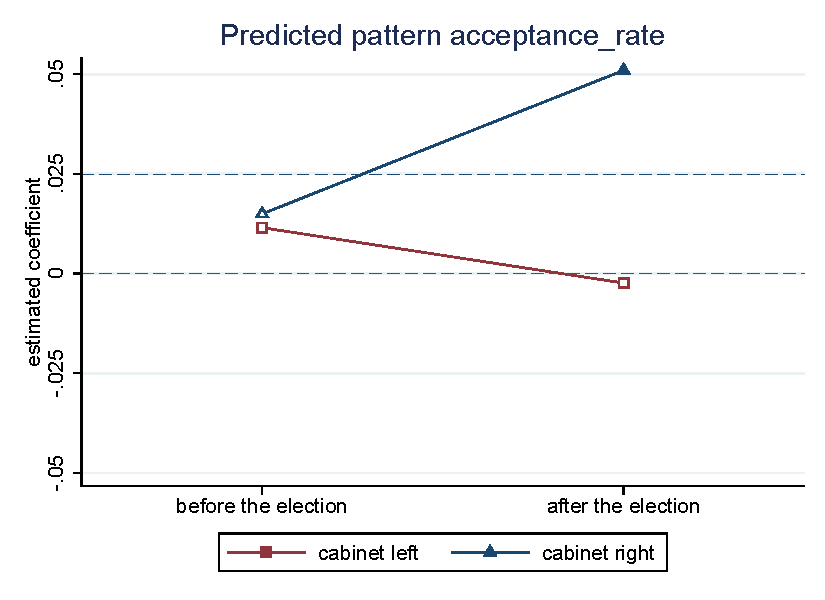
\includegraphics[width=1\textwidth]{figures_edited/acceptance_rate_graph1_R17.pdf}
	\caption{R17: Acceptance Rate: Predicted Pattern}
\end{figure}

\begin{table}[!ht]\centering
	\renewcommand{\arraystretch}{1.25}
	\def\sym#1{\ifmmode^{#1}\else\(^{#1}\)\fi}
	\caption{R17: Acceptance Rate: Predicted Pattern}
	\begin{tabular}{l*{2}{c}}
		\hline\hline
		                    &\multicolumn{1}{c}{(1)}&\multicolumn{1}{c}{(2)}\\
                    &\multicolumn{1}{c}{left}&\multicolumn{1}{c}{right}\\
\hline
before              &      0.0137\sym{*}  &     -0.0101         \\
                    &   (0.00571)         &   (0.00720)         \\
after               &    -0.00229         &      0.0267\sym{***}\\
                    &   (0.00611)         &   (0.00578)         \\
\hline
Observations        &       18331         &       18331         \\

		\hline\hline
		\multicolumn{3}{c}{\footnotesize Standard errors in parentheses} \\
		\multicolumn{3}{c}{\footnotesize (\sym{*} \(p<0.05\), \sym{**} \(p<0.01\), \sym{***} \(p<0.001\))}\\
	\end{tabular}
\end{table}

\clearpage
\textbf{R17: Use all destination countries with a maximum of two years missing decision data - Model 2}
\begin{figure}[!ht]
	\centering
	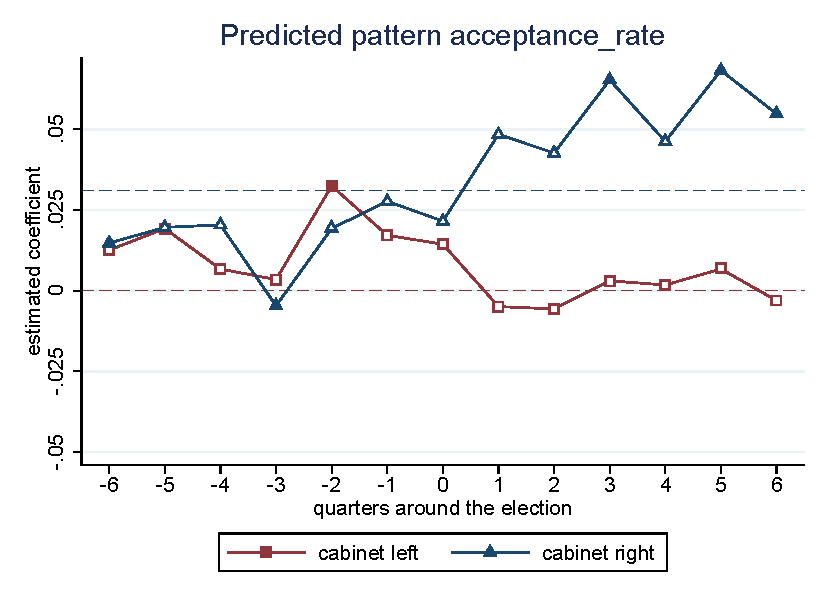
\includegraphics[width=0.7\textwidth]{figures_edited/acceptance_rate_graph2_R17.pdf}
	\caption{R17: Acceptance Rate: Predicted Pattern}
\end{figure}

\begin{table}[!ht]\centering
	\footnotesize
	\renewcommand{\arraystretch}{1.15}
	\def\sym#1{\ifmmode^{#1}\else\(^{#1}\)\fi}
	\caption{R17: Acceptance Rate: Predicted Pattern}
	\begin{tabular}{l*{2}{c}}
		\hline\hline
		                    &\multicolumn{1}{c}{(1)}&\multicolumn{1}{c}{(2)}\\
                    &\multicolumn{1}{c}{left}&\multicolumn{1}{c}{right}\\
\hline
 6 quarters before the election&      0.0126         &     -0.0163\sym{*}  \\
                    &   (0.00995)         &   (0.00815)         \\
 5 quarters before the election&      0.0192         &     -0.0114         \\
                    &    (0.0102)         &   (0.00862)         \\
 4 quarters before the election&     0.00668         &     -0.0107         \\
                    &   (0.00999)         &   (0.00957)         \\
 3 quarters before the election&     0.00343         &     -0.0357\sym{**} \\
                    &    (0.0129)         &    (0.0124)         \\
 2 quarters before the election&      0.0324\sym{***}&     -0.0118         \\
                    &   (0.00890)         &    (0.0108)         \\
 1 quarters before the election&      0.0171         &    -0.00335         \\
                    &   (0.00940)         &   (0.00990)         \\
Quarter of the election&      0.0144         &    -0.00950         \\
                    &   (0.00928)         &    (0.0132)         \\
 1 quarters after the election&    -0.00495         &      0.0174         \\
                    &   (0.00841)         &    (0.0118)         \\
 2 quarters after the election&    -0.00566         &      0.0116         \\
                    &   (0.00862)         &   (0.00982)         \\
 3 quarters after the election&     0.00305         &      0.0342\sym{**} \\
                    &   (0.00824)         &    (0.0107)         \\
 4 quarters after the election&     0.00174         &      0.0152         \\
                    &    (0.0107)         &   (0.00807)         \\
 5 quarters after the election&     0.00671         &      0.0372\sym{***}\\
                    &    (0.0102)         &    (0.0108)         \\
 6 quarters after the election&    -0.00305         &      0.0237\sym{**} \\
                    &    (0.0107)         &   (0.00809)         \\
\hline
Observations        &       18331         &       18331         \\

		\hline\hline
		\multicolumn{3}{c}{\footnotesize Standard errors in parentheses} \\
		\multicolumn{3}{c}{\footnotesize (\sym{*} \(p<0.05\), \sym{**} \(p<0.01\), \sym{***} \(p<0.001\))} \\
	\end{tabular}
\end{table}


% ===============================================================================================================


\clearpage
\FloatBarrier
\subsubsection{Use only destination countries that report decision data in all years}
\begin{table}[!ht]\centering
	\renewcommand{\arraystretch}{1.25}
	\small
	\def\sym#1{\ifmmode^{#1}\else\(^{#1}\)\fi}
	\caption{R18: Determinants of acceptance rate}
	\begin{tabular}{l*{3}{c}}
		\hline\hline
		                                        &\multicolumn{1}{c}{(1)}         &\multicolumn{1}{c}{(2)}         &\multicolumn{1}{c}{(3)}         \\
\hline
Political Terror Scale                  &    0.0213         &    0.0219         &                   \\
                                        &  (0.0110)         &  (0.0112)         &                   \\
Civic Liberty (FHI)                     &    0.0770\sym{***}&    0.0727\sym{**} &                   \\
                                        &  (0.0216)         &  (0.0219)         &                   \\
Political Rights (FHI)                  &   -0.0193         &   -0.0177         &                   \\
                                        &  (0.0145)         &  (0.0146)         &                   \\
Quarterly civil war battle death (000s) &    0.0464\sym{***}&    0.0462\sym{***}&                   \\
                                        & (0.00522)         & (0.00572)         &                   \\
Log origin country real GDP per capita  &   -0.0506         &   -0.0455         &                   \\
                                        &  (0.0319)         &  (0.0345)         &                   \\
Log migrant stock in 2000/1             & -0.000936         &                   & -0.000863         \\
                                        & (0.00362)         &                   & (0.00352)         \\
Log distance from origin to destination &   -0.0305         &                   &   -0.0225         \\
                                        &  (0.0377)         &                   &  (0.0355)         \\
Log destination country real GDP per capita&    -0.352\sym{*}  &    -0.283         &    -0.326         \\
                                        &   (0.167)         &   (0.175)         &   (0.171)         \\
Quarterly unemployment rate at destination&   -0.0163\sym{***}&   -0.0150\sym{**} &   -0.0152\sym{***}\\
                                        & (0.00421)         & (0.00460)         & (0.00408)         \\
Log average past total asylum decisions per capita&    -121.0\sym{*}  &    -130.3\sym{*}  &    -129.7\sym{*}  \\
                                        &   (49.80)         &   (50.18)         &   (48.59)         \\
Log average past dyadic asylum decisions per capita&     47.22         &     388.8         &    -104.6         \\
                                        &   (312.8)         &   (215.9)         &   (354.9)         \\
Weighted cabinet position right         &    0.0222         &    0.0264\sym{*}  &    0.0184         \\
                                        &  (0.0138)         &  (0.0128)         &  (0.0137)         \\
Cabinet position left * Before the election&    0.0342\sym{*}  &    0.0399\sym{**} &    0.0337\sym{**} \\
                                        &  (0.0131)         &  (0.0126)         &  (0.0124)         \\
Cabinet position left * After the election&   0.00206         &   0.00310         &  -0.00176         \\
                                        & (0.00945)         & (0.00996)         &  (0.0101)         \\
Cabinet position right * Before the election&    0.0212\sym{*}  &    0.0184\sym{*}  &    0.0222\sym{*}  \\
                                        & (0.00927)         & (0.00904)         & (0.00976)         \\
Cabinet position right * After the election&    0.0380\sym{**} &    0.0372\sym{**} &    0.0362\sym{**} \\
                                        &  (0.0120)         &  (0.0115)         &  (0.0112)         \\
\hline
Observations                            &      8567         &      8567         &      8567         \\
Adjusted \(R^{2}\)                      &     0.156         &     0.130         &     0.083         \\
Fixed Effects                           &         O         &     D x O         &     O x T         \\
Destination dummies                     &       Yes         &        No         &       Yes         \\
Quarter-Year dummies                    &       Yes         &       Yes         &        No         \\

		\hline\hline
		\multicolumn{4}{l}{\footnotesize Standard errors in parentheses (\sym{*} \(p<0.05\), \sym{**} \(p<0.01\), \sym{***} \(p<0.001\))}\\
	\end{tabular}
\end{table}

\clearpage
\textbf{R18: Use only destination countries that report decision data in all years - Model 1}
\begin{figure}[!ht]
	\centering
	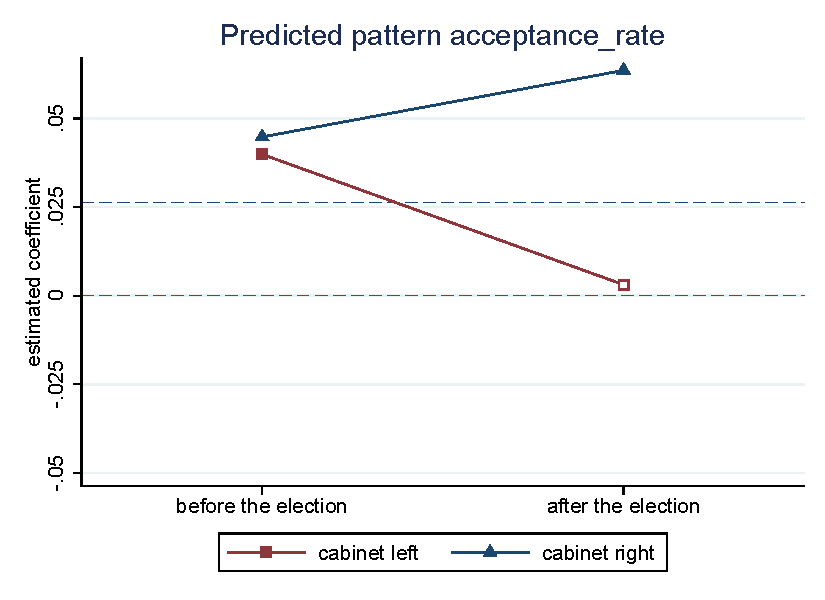
\includegraphics[width=1\textwidth]{figures_edited/acceptance_rate_graph1_R18.pdf}
	\caption{R18: Acceptance Rate: Predicted Pattern}
\end{figure}

\begin{table}[!ht]\centering
	\renewcommand{\arraystretch}{1.25}
	\def\sym#1{\ifmmode^{#1}\else\(^{#1}\)\fi}
	\caption{R18: Acceptance Rate: Predicted Pattern}
	\begin{tabular}{l*{2}{c}}
		\hline\hline
		                    &\multicolumn{1}{c}{(1)}&\multicolumn{1}{c}{(2)}\\
                    &\multicolumn{1}{c}{left}&\multicolumn{1}{c}{right}\\
\hline
before              &      0.0399\sym{**} &      0.0184\sym{*}  \\
                    &    (0.0126)         &   (0.00904)         \\
after               &     0.00310         &      0.0372\sym{**} \\
                    &   (0.00996)         &    (0.0115)         \\
\hline
Observations        &        8567         &        8567         \\

		\hline\hline
		\multicolumn{3}{c}{\footnotesize Standard errors in parentheses} \\
		\multicolumn{3}{c}{\footnotesize (\sym{*} \(p<0.05\), \sym{**} \(p<0.01\), \sym{***} \(p<0.001\))}\\
	\end{tabular}
\end{table}

\clearpage
\textbf{R18: Use only destination countries that report decision data in all years - Model 2}
\begin{figure}[!ht]
	\centering
	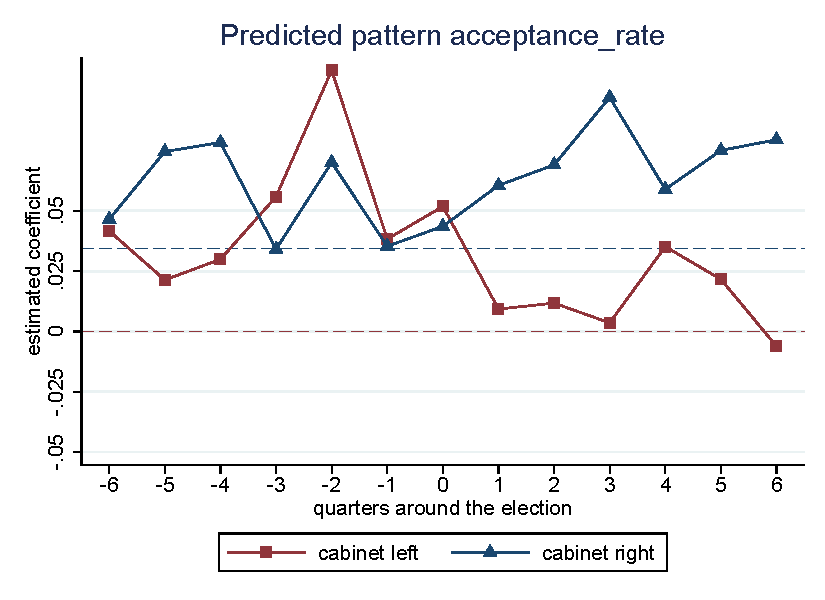
\includegraphics[width=0.7\textwidth]{figures_edited/acceptance_rate_graph2_R18.pdf}
	\caption{R18: Acceptance Rate: Predicted Pattern}
\end{figure}

\begin{table}[!ht]\centering
	\footnotesize
	\renewcommand{\arraystretch}{1.2}
	\def\sym#1{\ifmmode^{#1}\else\(^{#1}\)\fi}
	\caption{R18: Acceptance Rate: Predicted Pattern}
	\begin{tabular}{l*{2}{c}}
		\hline\hline
		                    &\multicolumn{1}{c}{(1)}&\multicolumn{1}{c}{(2)}\\
                    &\multicolumn{1}{c}{left}&\multicolumn{1}{c}{right}\\
\hline
 6 quarters before the election&      0.0417\sym{*}  &      0.0120         \\
                    &    (0.0208)         &    (0.0158)         \\
 5 quarters before the election&      0.0214         &      0.0401\sym{**} \\
                    &    (0.0173)         &    (0.0155)         \\
 4 quarters before the election&      0.0299\sym{*}  &      0.0439\sym{**} \\
                    &    (0.0146)         &    (0.0151)         \\
 3 quarters before the election&      0.0559\sym{*}  &   -0.000379         \\
                    &    (0.0221)         &    (0.0212)         \\
 2 quarters before the election&       0.108\sym{***}&      0.0356         \\
                    &    (0.0199)         &    (0.0188)         \\
 1 quarters before the election&      0.0383\sym{*}  &    0.000864         \\
                    &    (0.0183)         &    (0.0146)         \\
Quarter of the election&      0.0519\sym{***}&     0.00912         \\
                    &    (0.0143)         &    (0.0153)         \\
 1 quarters after the election&     0.00931         &      0.0261         \\
                    &    (0.0139)         &    (0.0165)         \\
 2 quarters after the election&      0.0118         &      0.0346         \\
                    &    (0.0154)         &    (0.0202)         \\
 3 quarters after the election&     0.00359         &      0.0626\sym{**} \\
                    &    (0.0146)         &    (0.0205)         \\
 4 quarters after the election&      0.0352         &      0.0245         \\
                    &    (0.0189)         &    (0.0174)         \\
 5 quarters after the election&      0.0217         &      0.0406\sym{*}  \\
                    &    (0.0135)         &    (0.0198)         \\
 6 quarters after the election&    -0.00613         &      0.0450\sym{*}  \\
                    &    (0.0170)         &    (0.0188)         \\
\hline
Observations        &        8567         &        8567         \\

		\hline\hline
		\multicolumn{3}{c}{\footnotesize Standard errors in parentheses} \\
		\multicolumn{3}{c}{\footnotesize (\sym{*} \(p<0.05\), \sym{**} \(p<0.01\), \sym{***} \(p<0.001\))} \\
	\end{tabular}
\end{table}



% ===============================================================================================================


\clearpage
\FloatBarrier
\subsubsection{Use only countries that are also in baseline application analysis}
\begin{table}[!ht]\centering
	\renewcommand{\arraystretch}{1.25}
	\small
	\def\sym#1{\ifmmode^{#1}\else\(^{#1}\)\fi}
	\caption{R19: Determinants of acceptance rate}
	\begin{tabular}{l*{3}{c}}
		\hline\hline
		                                        &\multicolumn{1}{c}{(1)}         &\multicolumn{1}{c}{(2)}         &\multicolumn{1}{c}{(3)}         \\
\hline
Political Terror Scale                  &    0.0252\sym{*}  &    0.0270\sym{*}  &                   \\
                                        &  (0.0107)         &  (0.0110)         &                   \\
Civic Liberty (FHI)                     &    0.0368         &    0.0339         &                   \\
                                        &  (0.0220)         &  (0.0220)         &                   \\
Political Rights (FHI)                  &  -0.00839         &  -0.00815         &                   \\
                                        &  (0.0185)         &  (0.0200)         &                   \\
Quarterly civil war battle death (000s) &    0.0515\sym{***}&    0.0513\sym{***}&                   \\
                                        & (0.00479)         & (0.00559)         &                   \\
Log origin country real GDP per capita  &   -0.0185         &   -0.0198         &                   \\
                                        &  (0.0288)         &  (0.0334)         &                   \\
Log migrant stock in 2000/1             &  0.000112         &                   &  0.000759         \\
                                        & (0.00246)         &                   & (0.00249)         \\
Log distance from origin to destination &   -0.0108         &                   &   -0.0157         \\
                                        &  (0.0191)         &                   &  (0.0188)         \\
Log destination country real GDP per capita&     0.215\sym{*}  &     0.232\sym{*}  &     0.244\sym{**} \\
                                        &  (0.0837)         &  (0.0873)         &  (0.0724)         \\
Quarterly unemployment rate at destination&  0.000446         &  0.000116         &  0.000403         \\
                                        & (0.00138)         & (0.00116)         & (0.00145)         \\
Log average past total asylum decisions per capita&    -78.14         &    -88.16         &    -67.48         \\
                                        &   (43.93)         &   (44.88)         &   (45.15)         \\
Log average past dyadic asylum decisions per capita&     458.2\sym{**} &     438.5         &     196.7         \\
                                        &   (142.5)         &   (271.9)         &   (144.3)         \\
Weighted cabinet position right         &    0.0312\sym{*}  &    0.0322\sym{*}  &    0.0311\sym{*}  \\
                                        &  (0.0124)         &  (0.0127)         &  (0.0128)         \\
Cabinet position left * Before the election&    0.0236\sym{**} &    0.0245\sym{***}&    0.0210\sym{**} \\
                                        & (0.00698)         & (0.00698)         & (0.00746)         \\
Cabinet position left * After the election&  -0.00795         &  -0.00810         &  -0.00724         \\
                                        & (0.00607)         & (0.00629)         & (0.00590)         \\
Cabinet position right * Before the election&   -0.0239\sym{*}  &   -0.0248\sym{**} &   -0.0234\sym{*}  \\
                                        & (0.00909)         & (0.00898)         & (0.00927)         \\
Cabinet position right * After the election&    0.0372\sym{***}&    0.0356\sym{***}&    0.0369\sym{***}\\
                                        & (0.00732)         & (0.00713)         & (0.00790)         \\
\hline
Observations                            &     12921         &     12921         &     12921         \\
Adjusted \(R^{2}\)                      &     0.144         &     0.137         &     0.056         \\
Fixed Effects                           &         O         &     D x O         &     O x T         \\
Destination dummies                     &       Yes         &        No         &       Yes         \\
Quarter-Year dummies                    &       Yes         &       Yes         &        No         \\

		\hline\hline
		\multicolumn{4}{l}{\footnotesize Standard errors in parentheses (\sym{*} \(p<0.05\), \sym{**} \(p<0.01\), \sym{***} \(p<0.001\))}\\
	\end{tabular}
\end{table}

\clearpage
\textbf{R19: Use only countries that are also in baseline application analysis - Model 1}
\begin{figure}[!ht]
	\centering
	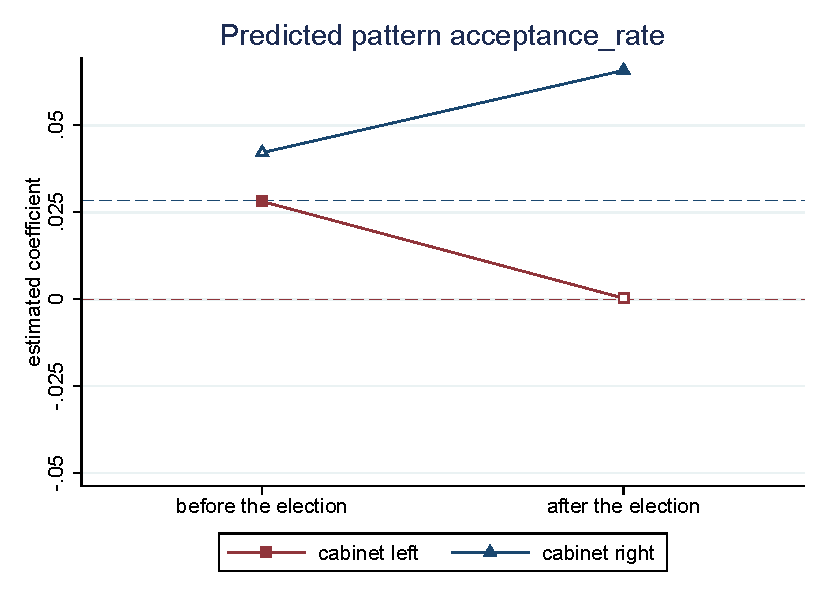
\includegraphics[width=1\textwidth]{figures_edited/acceptance_rate_graph1_R19.pdf}
	\caption{R19: Acceptance Rate: Predicted Pattern}
\end{figure}

\begin{table}[!ht]\centering
	\renewcommand{\arraystretch}{1.25}
	\def\sym#1{\ifmmode^{#1}\else\(^{#1}\)\fi}
	\caption{R19: Acceptance Rate: Predicted Pattern}
	\begin{tabular}{l*{2}{c}}
		\hline\hline
		                    &\multicolumn{1}{c}{(1)}&\multicolumn{1}{c}{(2)}\\
                    &\multicolumn{1}{c}{left}&\multicolumn{1}{c}{right}\\
\hline
before              &      0.0245\sym{***}&     -0.0248\sym{**} \\
                    &   (0.00698)         &   (0.00898)         \\
after               &    -0.00810         &      0.0356\sym{***}\\
                    &   (0.00629)         &   (0.00713)         \\
\hline
Observations        &       12921         &       12921         \\

		\hline\hline
		\multicolumn{3}{c}{\footnotesize Standard errors in parentheses} \\
		\multicolumn{3}{c}{\footnotesize (\sym{*} \(p<0.05\), \sym{**} \(p<0.01\), \sym{***} \(p<0.001\))}\\
	\end{tabular}
\end{table}

\clearpage
\textbf{R19: Use only countries that are also in baseline application analysis - Model 2}
\begin{figure}[!ht]
	\centering
	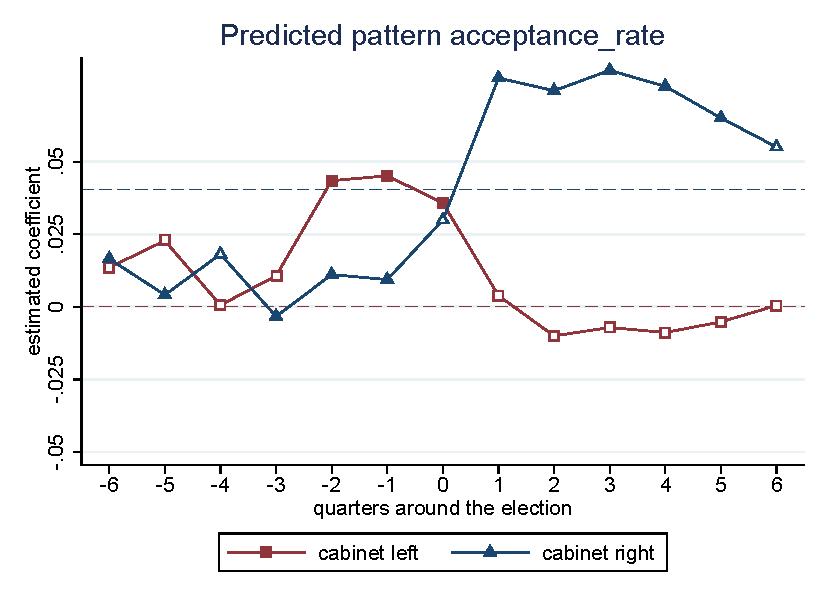
\includegraphics[width=0.7\textwidth]{figures_edited/acceptance_rate_graph2_R19.pdf}
	\caption{R19: Acceptance Rate: Predicted Pattern}
\end{figure}

\begin{table}[!ht]\centering
	\footnotesize
	\renewcommand{\arraystretch}{1.2}
	\def\sym#1{\ifmmode^{#1}\else\(^{#1}\)\fi}
	\caption{R19: Acceptance Rate: Predicted Pattern}
	\begin{tabular}{l*{2}{c}}
		\hline\hline
		                    &\multicolumn{1}{c}{(1)}&\multicolumn{1}{c}{(2)}\\
                    &\multicolumn{1}{c}{left}&\multicolumn{1}{c}{right}\\
\hline
 6 quarters before the election&      0.0135         &     -0.0237\sym{*}  \\
                    &   (0.00935)         &   (0.00967)         \\
 5 quarters before the election&      0.0228         &     -0.0361\sym{***}\\
                    &    (0.0127)         &   (0.00978)         \\
 4 quarters before the election&    0.000602         &     -0.0221         \\
                    &    (0.0124)         &    (0.0117)         \\
 3 quarters before the election&      0.0107         &     -0.0435\sym{***}\\
                    &    (0.0131)         &    (0.0125)         \\
 2 quarters before the election&      0.0435\sym{***}&     -0.0291\sym{*}  \\
                    &   (0.00977)         &    (0.0131)         \\
 1 quarters before the election&      0.0451\sym{***}&     -0.0309\sym{*}  \\
                    &    (0.0103)         &    (0.0152)         \\
Quarter of the election&      0.0357\sym{**} &     -0.0104         \\
                    &    (0.0120)         &    (0.0156)         \\
 1 quarters after the election&     0.00385         &      0.0385\sym{*}  \\
                    &   (0.00986)         &    (0.0168)         \\
 2 quarters after the election&    -0.01000         &      0.0342\sym{*}  \\
                    &    (0.0109)         &    (0.0148)         \\
 3 quarters after the election&    -0.00710         &      0.0412\sym{***}\\
                    &   (0.00834)         &    (0.0111)         \\
 4 quarters after the election&    -0.00882         &      0.0357\sym{***}\\
                    &   (0.00839)         &   (0.00943)         \\
 5 quarters after the election&    -0.00518         &      0.0248\sym{*}  \\
                    &   (0.00979)         &    (0.0119)         \\
 6 quarters after the election&    0.000472         &      0.0148         \\
                    &    (0.0127)         &    (0.0101)         \\
\hline
Observations        &       12921         &       12921         \\

		\hline\hline
		\multicolumn{3}{c}{\footnotesize Standard errors in parentheses} \\
		\multicolumn{3}{c}{\footnotesize (\sym{*} \(p<0.05\), \sym{**} \(p<0.01\), \sym{***} \(p<0.001\))} \\
	\end{tabular}
\end{table}


% ===============================================================================================================


\clearpage
\FloatBarrier
\subsubsection{Use only countries with a maximum of one early elections}
\begin{table}[!ht]\centering
	\renewcommand{\arraystretch}{1.25}
	\small
	\def\sym#1{\ifmmode^{#1}\else\(^{#1}\)\fi}
	\caption{R20: Determinants of acceptance rate}
	\begin{tabular}{l*{3}{c}}
		\hline\hline
		                                        &\multicolumn{1}{c}{(1)}         &\multicolumn{1}{c}{(2)}         &\multicolumn{1}{c}{(3)}         \\
\hline
Political Terror Scale                  &    0.0207         &    0.0235\sym{*}  &                   \\
                                        &  (0.0106)         &  (0.0106)         &                   \\
Civic Liberty (FHI)                     &    0.0413         &    0.0381         &                   \\
                                        &  (0.0208)         &  (0.0206)         &                   \\
Political Rights (FHI)                  &   -0.0124         &  -0.00992         &                   \\
                                        &  (0.0181)         &  (0.0185)         &                   \\
Quarterly civil war battle death (000s) &    0.0531\sym{***}&    0.0516\sym{***}&                   \\
                                        & (0.00523)         & (0.00593)         &                   \\
Log origin country real GDP per capita  &   -0.0227         &   -0.0266         &                   \\
                                        &  (0.0287)         &  (0.0326)         &                   \\
Log migrant stock in 2000/1             &   0.00364         &                   &   0.00440         \\
                                        & (0.00243)         &                   & (0.00245)         \\
Log distance from origin to destination &    0.0135         &                   &    0.0161         \\
                                        &  (0.0252)         &                   &  (0.0252)         \\
Log destination country real GDP per capita&     0.129         &     0.166         &     0.130         \\
                                        &  (0.0894)         &  (0.0932)         &  (0.0826)         \\
Quarterly unemployment rate at destination&  -0.00107         & -0.000846         &  -0.00109         \\
                                        & (0.00144)         & (0.00132)         & (0.00146)         \\
Log average past total asylum decisions per capita&    -39.90         &    -59.66         &    -26.35         \\
                                        &   (41.58)         &   (44.16)         &   (40.70)         \\
Log average past dyadic asylum decisions per capita&     188.1         &     418.0         &    -13.76         \\
                                        &   (147.7)         &   (252.3)         &   (145.7)         \\
Weighted cabinet position right         &    0.0102         &    0.0133         &   0.00897         \\
                                        &  (0.0118)         &  (0.0123)         &  (0.0128)         \\
Cabinet position left * Before the election&    0.0198\sym{*}  &    0.0230\sym{**} &    0.0186\sym{*}  \\
                                        & (0.00767)         & (0.00755)         & (0.00779)         \\
Cabinet position left * After the election&   -0.0114         &   -0.0101         &   -0.0122         \\
                                        & (0.00633)         & (0.00646)         & (0.00658)         \\
Cabinet position right * Before the election&   -0.0228\sym{*}  &   -0.0227\sym{*}  &   -0.0228\sym{*}  \\
                                        & (0.00877)         & (0.00889)         & (0.00910)         \\
Cabinet position right * After the election&    0.0295\sym{***}&    0.0279\sym{***}&    0.0292\sym{***}\\
                                        & (0.00813)         & (0.00769)         & (0.00820)         \\
\hline
Observations                            &     13486         &     13486         &     13486         \\
Adjusted \(R^{2}\)                      &     0.148         &     0.128         &     0.061         \\
Fixed Effects                           &         O         &     D x O         &     O x T         \\
Destination dummies                     &       Yes         &        No         &       Yes         \\
Quarter-Year dummies                    &       Yes         &       Yes         &        No         \\

		\hline\hline
		\multicolumn{4}{l}{\footnotesize Standard errors in parentheses (\sym{*} \(p<0.05\), \sym{**} \(p<0.01\), \sym{***} \(p<0.001\))}\\
	\end{tabular}
\end{table}

\clearpage
\textbf{R20: Use only countries with a maximum of one early elections - Model1}
\begin{figure}[!ht]
	\centering
	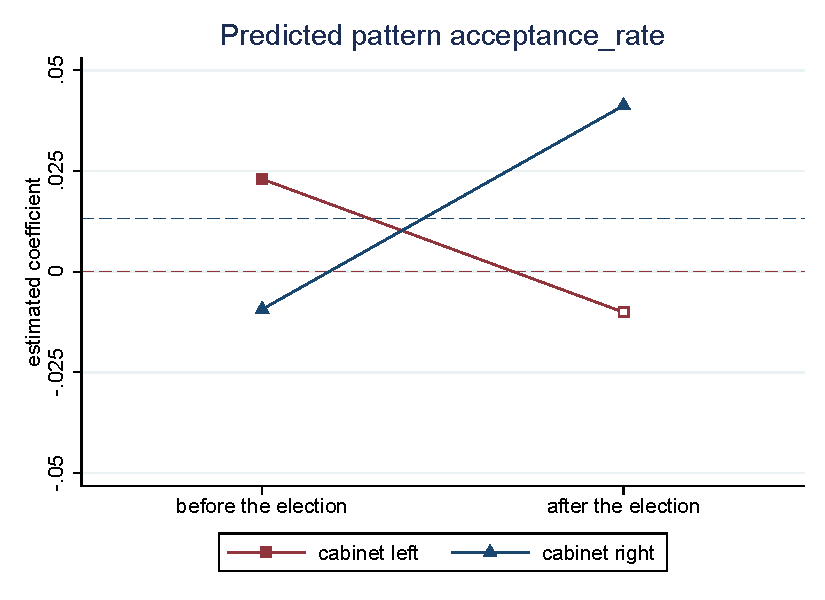
\includegraphics[width=1\textwidth]{figures_edited/acceptance_rate_graph1_R20.pdf}
	\caption{R20: Acceptance Rate: Predicted Pattern}
\end{figure}

\begin{table}[!ht]\centering
	\renewcommand{\arraystretch}{1.25}
	\def\sym#1{\ifmmode^{#1}\else\(^{#1}\)\fi}
	\caption{R20: Acceptance Rate: Predicted Pattern}
	\begin{tabular}{l*{2}{c}}
		\hline\hline
		                    &\multicolumn{1}{c}{(1)}&\multicolumn{1}{c}{(2)}\\
                    &\multicolumn{1}{c}{left}&\multicolumn{1}{c}{right}\\
\hline
before              &      0.0230\sym{**} &     -0.0227\sym{*}  \\
                    &   (0.00755)         &   (0.00889)         \\
after               &     -0.0101         &      0.0279\sym{***}\\
                    &   (0.00646)         &   (0.00769)         \\
\hline
Observations        &       13486         &       13486         \\

		\hline\hline
		\multicolumn{3}{c}{\footnotesize Standard errors in parentheses} \\
		\multicolumn{3}{c}{\footnotesize (\sym{*} \(p<0.05\), \sym{**} \(p<0.01\), \sym{***} \(p<0.001\))}\\
	\end{tabular}
\end{table}

\clearpage
\textbf{R20: Use only countries with a maximum of one early elections - Model2}
\begin{figure}[!ht]
	\centering
	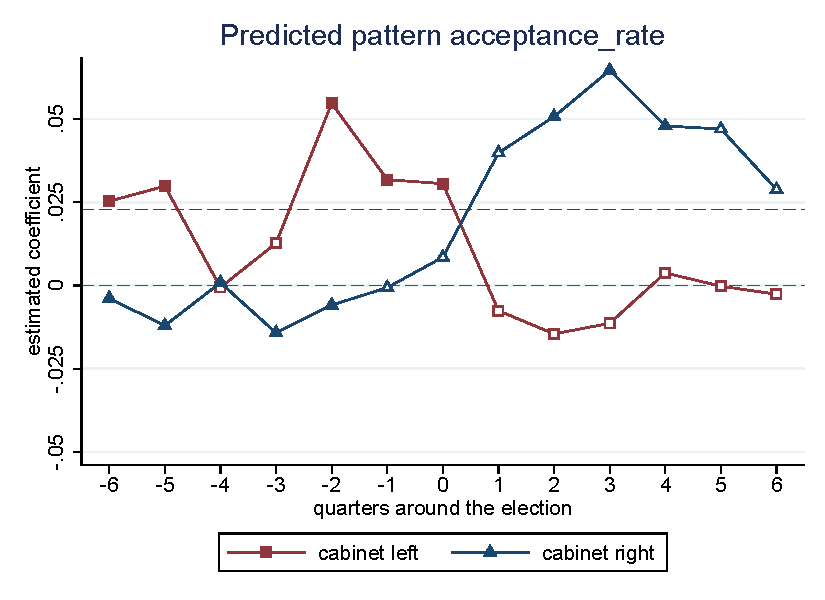
\includegraphics[width=0.7\textwidth]{figures_edited/acceptance_rate_graph2_R20.pdf}
	\caption{R20: Acceptance Rate: Predicted Pattern}
\end{figure}

\begin{table}[!ht]\centering
	\footnotesize
	\renewcommand{\arraystretch}{1.15}
	\def\sym#1{\ifmmode^{#1}\else\(^{#1}\)\fi}
	\caption{R20: Acceptance Rate: Predicted Pattern}
	\begin{tabular}{l*{2}{c}}
		\hline\hline
		                    &\multicolumn{1}{c}{(1)}&\multicolumn{1}{c}{(2)}\\
                    &\multicolumn{1}{c}{left}&\multicolumn{1}{c}{right}\\
\hline
 6 quarters before the election&      0.0253\sym{*}  &     -0.0267\sym{**} \\
                    &    (0.0105)         &    (0.0102)         \\
 5 quarters before the election&      0.0299\sym{*}  &     -0.0349\sym{***}\\
                    &    (0.0123)         &    (0.0102)         \\
 4 quarters before the election&   -0.000531         &     -0.0220\sym{*}  \\
                    &    (0.0107)         &    (0.0109)         \\
 3 quarters before the election&      0.0127         &     -0.0371\sym{**} \\
                    &    (0.0147)         &    (0.0125)         \\
 2 quarters before the election&      0.0547\sym{***}&     -0.0288\sym{*}  \\
                    &    (0.0118)         &    (0.0128)         \\
 1 quarters before the election&      0.0318\sym{**} &     -0.0235         \\
                    &    (0.0119)         &    (0.0134)         \\
Quarter of the election&      0.0306\sym{*}  &     -0.0144         \\
                    &    (0.0130)         &    (0.0155)         \\
 1 quarters after the election&    -0.00755         &      0.0169         \\
                    &    (0.0101)         &    (0.0132)         \\
 2 quarters after the election&     -0.0145         &      0.0278\sym{*}  \\
                    &   (0.00953)         &    (0.0119)         \\
 3 quarters after the election&     -0.0113         &      0.0417\sym{**} \\
                    &   (0.00857)         &    (0.0145)         \\
 4 quarters after the election&     0.00380         &      0.0250\sym{*}  \\
                    &    (0.0104)         &    (0.0106)         \\
 5 quarters after the election&   -0.000182         &      0.0241         \\
                    &    (0.0106)         &    (0.0133)         \\
 6 quarters after the election&    -0.00259         &     0.00597         \\
                    &    (0.0119)         &   (0.00990)         \\
\hline
Observations        &       13486         &       13486         \\

		\hline\hline
		\multicolumn{3}{c}{\footnotesize Standard errors in parentheses} \\
		\multicolumn{3}{c}{\footnotesize (\sym{*} \(p<0.05\), \sym{**} \(p<0.01\), \sym{***} \(p<0.001\))} \\
	\end{tabular}
\end{table}


% ===============================================================================================================


\clearpage
\FloatBarrier
\subsubsection{Use only countries with no early elections}
\begin{table}[!ht]\centering
	\renewcommand{\arraystretch}{1.25}
	\small
	\def\sym#1{\ifmmode^{#1}\else\(^{#1}\)\fi}
	\caption{R21: Determinants of acceptance rate}
	\begin{tabular}{l*{3}{c}}
		\hline\hline
		                                        &\multicolumn{1}{c}{(1)}         &\multicolumn{1}{c}{(2)}         &\multicolumn{1}{c}{(3)}         \\
\hline
Political Terror Scale                  &   0.00886         &    0.0121         &                   \\
                                        &  (0.0147)         &  (0.0135)         &                   \\
Civic Liberty (FHI)                     &    0.0455\sym{*}  &    0.0435\sym{*}  &                   \\
                                        &  (0.0206)         &  (0.0204)         &                   \\
Political Rights (FHI)                  &   -0.0111         &  -0.00797         &                   \\
                                        &  (0.0167)         &  (0.0149)         &                   \\
Quarterly civil war battle death (000s) &    0.0491\sym{***}&    0.0464\sym{***}&                   \\
                                        & (0.00693)         & (0.00691)         &                   \\
Log origin country real GDP per capita  &   -0.0240         &   -0.0292         &                   \\
                                        &  (0.0234)         &  (0.0254)         &                   \\
Log migrant stock in 2000/1             &   0.00634\sym{*}  &                   &   0.00709\sym{*}  \\
                                        & (0.00296)         &                   & (0.00305)         \\
Log distance from origin to destination &    0.0249         &                   &    0.0289         \\
                                        &  (0.0453)         &                   &  (0.0443)         \\
Log destination country real GDP per capita&     0.115         &     0.142         &     0.138         \\
                                        &  (0.0885)         &  (0.0881)         &  (0.0937)         \\
Quarterly unemployment rate at destination&  -0.00485         &  -0.00358         &  -0.00583         \\
                                        & (0.00331)         & (0.00311)         & (0.00340)         \\
Log average past total asylum decisions per capita&    -52.06         &    -69.07         &    -36.32         \\
                                        &   (43.63)         &   (46.57)         &   (43.50)         \\
Log average past dyadic asylum decisions per capita&     181.8         &     482.4\sym{*}  &    -13.16         \\
                                        &   (139.5)         &   (206.8)         &   (147.7)         \\
Weighted cabinet position right         &    0.0114         &    0.0174         &   0.00396         \\
                                        &  (0.0164)         &  (0.0166)         &  (0.0174)         \\
Cabinet position left * Before the election&    0.0137         &    0.0196\sym{*}  &    0.0111         \\
                                        & (0.00847)         & (0.00794)         & (0.00895)         \\
Cabinet position left * After the election&   -0.0167         &   -0.0139         &   -0.0192\sym{*}  \\
                                        & (0.00894)         & (0.00893)         & (0.00910)         \\
Cabinet position right * Before the election&   -0.0409\sym{***}&   -0.0396\sym{***}&   -0.0421\sym{***}\\
                                        & (0.00956)         & (0.00975)         &  (0.0103)         \\
Cabinet position right * After the election&    0.0211\sym{*}  &    0.0201\sym{*}  &    0.0229\sym{*}  \\
                                        & (0.00900)         & (0.00851)         &  (0.0103)         \\
\hline
Observations                            &      9363         &      9363         &      9363         \\
Adjusted \(R^{2}\)                      &     0.142         &     0.116         &     0.070         \\
Fixed Effects                           &         O         &     D x O         &     O x T         \\
Destination dummies                     &       Yes         &        No         &       Yes         \\
Quarter-Year dummies                    &       Yes         &       Yes         &        No         \\

		\hline\hline
		\multicolumn{4}{l}{\footnotesize Standard errors in parentheses (\sym{*} \(p<0.05\), \sym{**} \(p<0.01\), \sym{***} \(p<0.001\))}\\
	\end{tabular}
\end{table}

\clearpage
\textbf{R21: Use only countries with no early elections - Model1}
\begin{figure}[!ht]
	\centering
	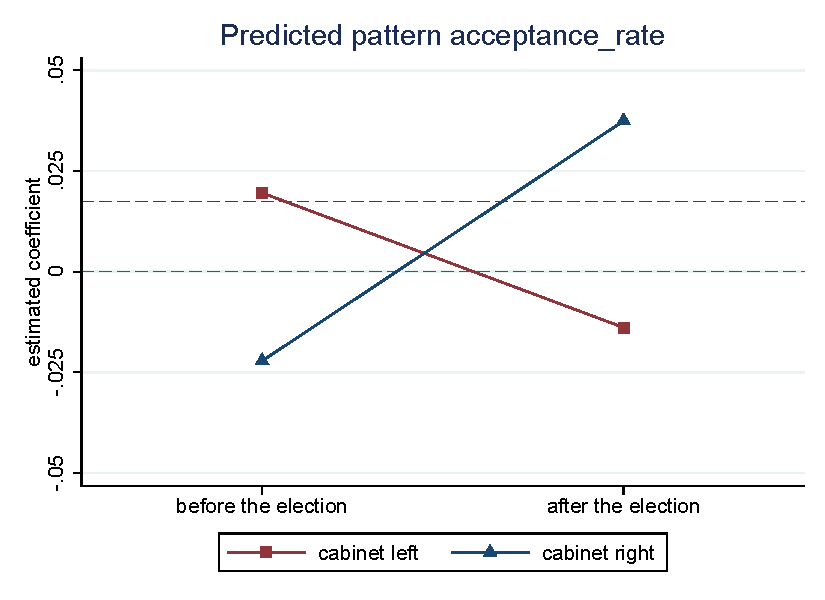
\includegraphics[width=1\textwidth]{figures_edited/acceptance_rate_graph1_R21.pdf}
	\caption{R21: Acceptance Rate: Predicted Pattern}
\end{figure}

\begin{table}[!ht]\centering
	\renewcommand{\arraystretch}{1.25}
	\def\sym#1{\ifmmode^{#1}\else\(^{#1}\)\fi}
	\caption{R21: Acceptance Rate: Predicted Pattern}
	\begin{tabular}{l*{2}{c}}
		\hline\hline
		                    &\multicolumn{1}{c}{(1)}&\multicolumn{1}{c}{(2)}\\
                    &\multicolumn{1}{c}{left}&\multicolumn{1}{c}{right}\\
\hline
before              &      0.0196\sym{*}  &     -0.0396\sym{***}\\
                    &   (0.00794)         &   (0.00975)         \\
after               &     -0.0139         &      0.0201\sym{*}  \\
                    &   (0.00893)         &   (0.00851)         \\
\hline
Observations        &        9363         &        9363         \\

		\hline\hline
		\multicolumn{3}{c}{\footnotesize Standard errors in parentheses} \\
		\multicolumn{3}{c}{\footnotesize (\sym{*} \(p<0.05\), \sym{**} \(p<0.01\), \sym{***} \(p<0.001\))}\\
	\end{tabular}
\end{table}

\clearpage
\textbf{R21: Use only countries with no early elections - Model2}
\begin{figure}[!ht]
	\centering
	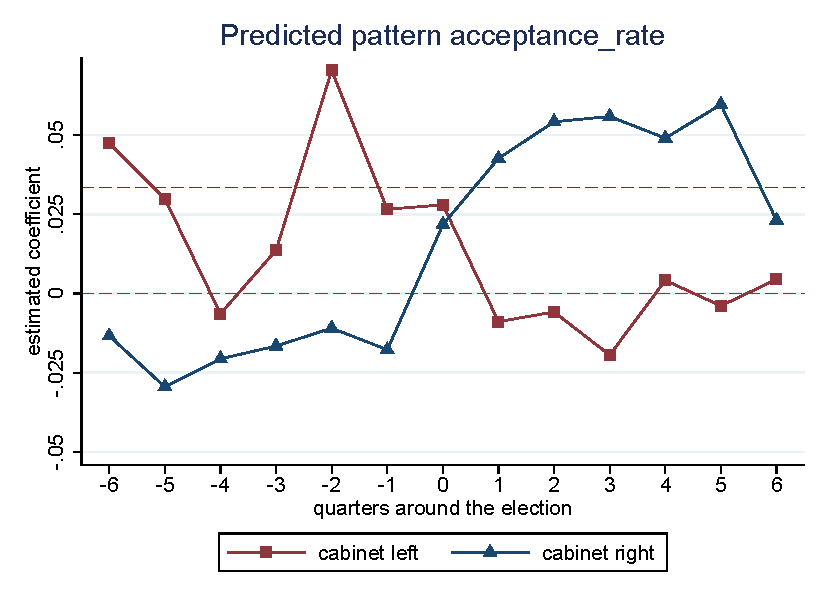
\includegraphics[width=0.7\textwidth]{figures_edited/acceptance_rate_graph2_R21.pdf}
	\caption{R21: Acceptance Rate: Predicted Pattern}
\end{figure}

\begin{table}[!ht]\centering
	\footnotesize
	\renewcommand{\arraystretch}{1.15}
	\def\sym#1{\ifmmode^{#1}\else\(^{#1}\)\fi}
	\caption{R21: Acceptance Rate: Predicted Pattern}
	\begin{tabular}{l*{2}{c}}
		\hline\hline
		                    &\multicolumn{1}{c}{(1)}&\multicolumn{1}{c}{(2)}\\
                    &\multicolumn{1}{c}{left}&\multicolumn{1}{c}{right}\\
\hline
 6 quarters before the election&      0.0474\sym{***}&     -0.0468\sym{***}\\
                    &    (0.0121)         &    (0.0110)         \\
 5 quarters before the election&      0.0299\sym{**} &     -0.0629\sym{***}\\
                    &    (0.0115)         &    (0.0151)         \\
 4 quarters before the election&    -0.00634         &     -0.0541\sym{***}\\
                    &    (0.0117)         &    (0.0133)         \\
 3 quarters before the election&      0.0137         &     -0.0500\sym{***}\\
                    &    (0.0159)         &    (0.0136)         \\
 2 quarters before the election&      0.0704\sym{***}&     -0.0444\sym{**} \\
                    &    (0.0143)         &    (0.0154)         \\
 1 quarters before the election&      0.0266         &     -0.0512\sym{***}\\
                    &    (0.0155)         &    (0.0152)         \\
Quarter of the election&      0.0280         &     -0.0117         \\
                    &    (0.0184)         &    (0.0186)         \\
 1 quarters after the election&    -0.00885         &     0.00916         \\
                    &    (0.0150)         &    (0.0204)         \\
 2 quarters after the election&    -0.00579         &      0.0207         \\
                    &    (0.0148)         &    (0.0165)         \\
 3 quarters after the election&     -0.0194         &      0.0224         \\
                    &    (0.0135)         &    (0.0145)         \\
 4 quarters after the election&     0.00417         &      0.0156         \\
                    &    (0.0155)         &    (0.0125)         \\
 5 quarters after the election&    -0.00386         &      0.0261         \\
                    &    (0.0120)         &    (0.0150)         \\
 6 quarters after the election&     0.00450         &     -0.0103         \\
                    &    (0.0135)         &    (0.0147)         \\
\hline
Observations        &        9363         &        9363         \\

		\hline\hline
		\multicolumn{3}{c}{\footnotesize Standard errors in parentheses} \\
		\multicolumn{3}{c}{\footnotesize (\sym{*} \(p<0.05\), \sym{**} \(p<0.01\), \sym{***} \(p<0.001\))} \\
	\end{tabular}
\end{table}
 % ===============================================================================================================
 % ===============================================================================================================

\clearpage
\FloatBarrier
\subsection{Heterogeneity by origin country region}
\begin{table}[!ht]\centering
	\renewcommand{\arraystretch}{1.25}
	\small
	\def\sym#1{\ifmmode^{#1}\else\(^{#1}\)\fi}
	\caption{Determinants of acceptance rate}
	\begin{tabular}{l*{4}{c}}
		\hline\hline
		                    &\multicolumn{1}{c}{(1)}         &\multicolumn{1}{c}{(2)}         &\multicolumn{1}{c}{(3)}         &\multicolumn{1}{c}{(4)}         \\
\hline
Political Terror Scale&      0.0638\sym{***}&      0.0214         &      0.0232\sym{*}  &      0.0134         \\
                    &   (0.00945)         &    (0.0189)         &   (0.00886)         &   (0.00775)         \\
Civic Liberty (FHI) &      0.0743\sym{*}  &      0.0161         &     0.00712         &    -0.00259         \\
                    &    (0.0236)         &    (0.0233)         &    (0.0225)         &    (0.0113)         \\
Political Rights (FHI)&     -0.0784\sym{**} &    -0.00757         &      0.0265\sym{**} &      0.0282\sym{*}  \\
                    &    (0.0148)         &    (0.0193)         &   (0.00665)         &    (0.0131)         \\
Quarterly civil war battle death (000s)&      0.0356\sym{***}&     0.00202         &      0.0520\sym{**} &      0.0164         \\
                    &   (0.00630)         &    (0.0173)         &    (0.0109)         &    (0.0143)         \\
Log origin country real GDP per capita&     0.00946         &     -0.0683\sym{*}  &      0.0424         &      0.0688\sym{**} \\
                    &    (0.0531)         &    (0.0299)         &    (0.0555)         &    (0.0208)         \\
Log destination country real GDP per capita&       0.143         &      0.0383         &       0.184\sym{**} &       0.150         \\
                    &     (0.173)         &    (0.0863)         &    (0.0543)         &     (0.178)         \\
Quarterly unemployment rate at destination&    -0.00523         &    -0.00304         &     0.00177         &    0.000991         \\
                    &   (0.00256)         &   (0.00186)         &   (0.00181)         &   (0.00181)         \\
Log average past total asylum decisions per capita&      -347.3\sym{**} &      -138.1\sym{*}  &       4.036         &      -183.5\sym{**} \\
                    &     (94.85)         &     (53.92)         &     (63.96)         &     (55.97)         \\
Log average past dyadic asylum decisions per capita&       673.2\sym{**} &       15.26         &      -748.6         &      -747.0\sym{*}  \\
                    &     (163.3)         &     (821.5)         &     (466.2)         &     (292.5)         \\
Weighted cabinet position right&     0.00475         &      0.0714\sym{**} &     -0.0171         &      0.0349         \\
                    &    (0.0136)         &    (0.0236)         &    (0.0148)         &    (0.0180)         \\
Cabinet position left * Before the election&     0.00307         &      0.0237         &     0.00706         &      0.0233\sym{*}  \\
                    &    (0.0117)         &    (0.0140)         &    (0.0124)         &   (0.00958)         \\
Cabinet position left * After the election&   -0.000343         &     0.00600         &    -0.00780         &      0.0111         \\
                    &   (0.00585)         &    (0.0114)         &    (0.0157)         &    (0.0101)         \\
Cabinet position right * Before the election&      0.0118         &     -0.0343         &    0.000432         &    -0.00492         \\
                    &    (0.0104)         &    (0.0180)         &    (0.0143)         &    (0.0134)         \\
Cabinet position right * After the election&      0.0227         &      0.0284\sym{**} &      0.0256         &      0.0341\sym{**} \\
                    &    (0.0160)         &   (0.00949)         &    (0.0121)         &   (0.00844)         \\
\hline
Observations        &        3176         &        5271         &        3592         &        5507         \\
Adjusted \(R^{2}\)  &       0.303         &       0.092         &       0.061         &       0.043         \\
Fixed Effects       &       D x O         &       D x O         &       D x O         &       D x O         \\
Destination dummies &          No         &          No         &          No         &          No         \\
Quarter-Year dummies&         Yes         &         Yes         &         Yes         &         Yes         \\
Area of origin      &        MENA         &      Africa         &         SEA         &         ECA         \\

		\hline\hline
		\multicolumn{5}{l}{\footnotesize Standard errors in parentheses (\sym{*} \(p<0.05\), \sym{**} \(p<0.01\), \sym{***} \(p<0.001\))}\\
	\end{tabular}
\end{table}

\clearpage
\textbf{Baseline Specification - Model 1 by region}
\begin{figure}[!ht]
	\centering
	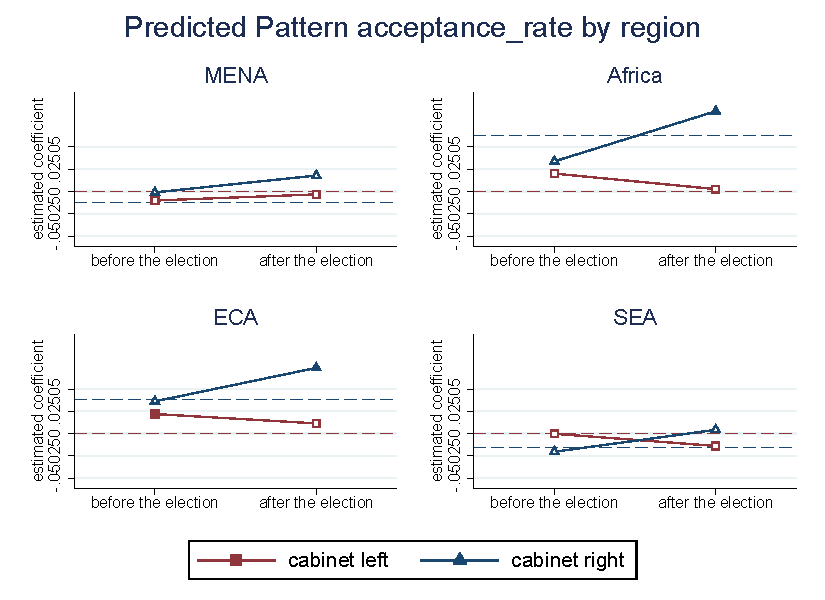
\includegraphics[width=0.8\textwidth]{figures_edited/acceptance_rate_graph1_by_region.pdf}
	\caption{Acceptance Rate: Predicted Pattern}
\end{figure}

\begin{table}[!ht]\centering
	\footnotesize
	\renewcommand{\arraystretch}{1.1}
	\def\sym#1{\ifmmode^{#1}\else\(^{#1}\)\fi}
	\caption{Acceptance Rate: Predicted Pattern}
	\begin{subtable}{.5\linewidth}
		\centering
		\caption{Middle East and North Africa}
		\begin{tabular}{l*{2}{c}}
			\hline\hline
			                    &\multicolumn{1}{c}{(1)}&\multicolumn{1}{c}{(2)}\\
                    &\multicolumn{1}{c}{left}&\multicolumn{1}{c}{right}\\
\hline
before              &     0.00307         &      0.0118         \\
                    &    (0.0117)         &    (0.0104)         \\
after               &   -0.000343         &      0.0227         \\
                    &   (0.00585)         &    (0.0160)         \\
\hline
Observations        &        3176         &        3176         \\

			\hline\hline
			\multicolumn{3}{c}{\footnotesize Standard errors in parentheses} \\
			\multicolumn{3}{c}{\footnotesize (\sym{*} \(p<0.05\), \sym{**} \(p<0.01\), \sym{***} \(p<0.001\))}\\
		\end{tabular}
	\end{subtable}%
	\begin{subtable}{.5\linewidth}
		\centering
		\caption{Africa}
		\begin{tabular}{l*{2}{c}}
			\hline\hline
			                    &\multicolumn{1}{c}{(1)}&\multicolumn{1}{c}{(2)}\\
                    &\multicolumn{1}{c}{left}&\multicolumn{1}{c}{right}\\
\hline
before              &      0.0237         &     -0.0343         \\
                    &    (0.0140)         &    (0.0180)         \\
after               &     0.00600         &      0.0284\sym{**} \\
                    &    (0.0114)         &   (0.00949)         \\
\hline
Observations        &        5271         &        5271         \\

			\hline\hline
			\multicolumn{3}{c}{\footnotesize Standard errors in parentheses} \\
			\multicolumn{3}{c}{\footnotesize (\sym{*} \(p<0.05\), \sym{**} \(p<0.01\), \sym{***} \(p<0.001\))}\\
		\end{tabular}
	\end{subtable}%
\end{table}

\begin{table}[!ht]\centering
	\footnotesize
	\renewcommand{\arraystretch}{1.1}
	\def\sym#1{\ifmmode^{#1}\else\(^{#1}\)\fi}
	\caption{Acceptance Rate: Predicted Pattern}
	\begin{subtable}{.5\linewidth}
		\centering
		\caption{Europe and Central Asia}
		\begin{tabular}{l*{2}{c}}
			\hline\hline
			                    &\multicolumn{1}{c}{(1)}&\multicolumn{1}{c}{(2)}\\
                    &\multicolumn{1}{c}{left}&\multicolumn{1}{c}{right}\\
\hline
before              &      0.0233\sym{*}  &    -0.00492         \\
                    &   (0.00958)         &    (0.0134)         \\
after               &      0.0111         &      0.0341\sym{***}\\
                    &    (0.0101)         &   (0.00844)         \\
\hline
Observations        &        5507         &        5507         \\

			\hline\hline
			\multicolumn{3}{c}{\footnotesize Standard errors in parentheses} \\
			\multicolumn{3}{c}{\footnotesize (\sym{*} \(p<0.05\), \sym{**} \(p<0.01\), \sym{***} \(p<0.001\))}\\
		\end{tabular}
	\end{subtable}%
	\begin{subtable}{.5\linewidth}
		\centering
		\caption{South and East Asia}
		\begin{tabular}{l*{2}{c}}
			\hline\hline
			                    &\multicolumn{1}{c}{(1)}&\multicolumn{1}{c}{(2)}\\
                    &\multicolumn{1}{c}{left}&\multicolumn{1}{c}{right}\\
\hline
before              &     0.00706         &    0.000432         \\
                    &    (0.0124)         &    (0.0143)         \\
after               &    -0.00780         &      0.0256\sym{*}  \\
                    &    (0.0157)         &    (0.0121)         \\
\hline
Observations        &        3592         &        3592         \\

			\hline\hline
			\multicolumn{3}{c}{\footnotesize Standard errors in parentheses} \\
			\multicolumn{3}{c}{\footnotesize (\sym{*} \(p<0.05\), \sym{**} \(p<0.01\), \sym{***} \(p<0.001\))}\\
		\end{tabular}
	\end{subtable}%
\end{table}

\clearpage
\textbf{Baseline Specification - Model 2 by region}

\begin{figure}[!ht]
	\centering
	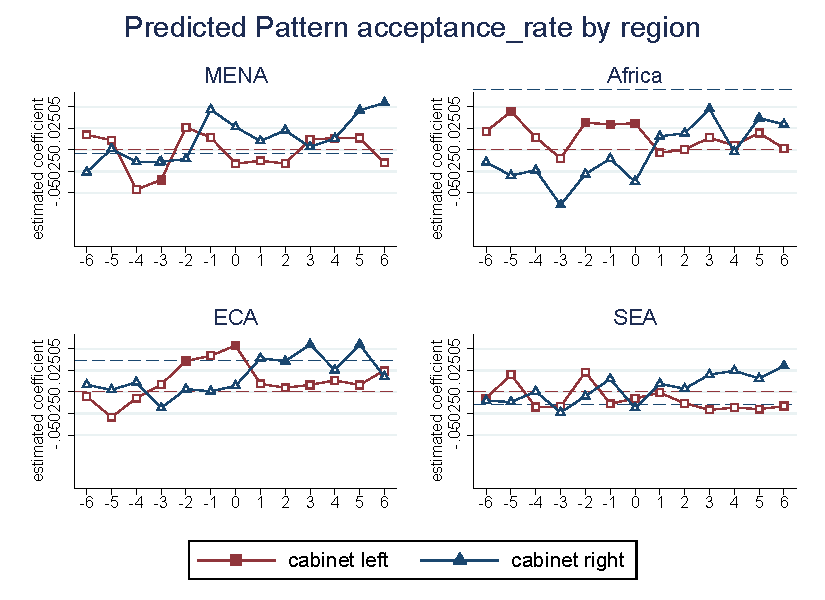
\includegraphics[width=0.7\textwidth]{figures_edited/acceptance_rate_graph2_by_region.pdf}
	\caption{Acceptance Rate: Predicted Pattern}
\end{figure}

\begin{table}[!ht]\centering
	\footnotesize
	\renewcommand{\arraystretch}{1.1}
	\def\sym#1{\ifmmode^{#1}\else\(^{#1}\)\fi}
	\caption{Acceptance Rate: Predicted Pattern}
	\begin{subtable}{.5\linewidth}
	\centering
	\caption{Middle East and North Africa}
	\begin{tabular}{l*{2}{c}}
		\hline\hline
		                    &\multicolumn{1}{c}{(1)}&\multicolumn{1}{c}{(2)}\\
                    &\multicolumn{1}{c}{left}&\multicolumn{1}{c}{right}\\
\hline
 6 quarters before the election&      0.0278         &     -0.0189         \\
                    &    (0.0200)         &    (0.0241)         \\
 5 quarters before the election&      0.0161         &   -0.000981         \\
                    &    (0.0262)         &    (0.0203)         \\
 4 quarters before the election&     -0.0424\sym{*}  &    -0.00438         \\
                    &    (0.0194)         &    (0.0277)         \\
 3 quarters before the election&     -0.0270         &     -0.0239         \\
                    &    (0.0176)         &    (0.0156)         \\
 2 quarters before the election&      0.0389         &     -0.0165         \\
                    &    (0.0287)         &    (0.0127)         \\
 1 quarters before the election&      0.0453\sym{*}  &      0.0421         \\
                    &    (0.0223)         &    (0.0285)         \\
Quarter of the election&     0.00213         &      0.0505\sym{*}  \\
                    &    (0.0195)         &    (0.0244)         \\
 1 quarters after the election&     -0.0107         &      0.0144         \\
                    &    (0.0154)         &    (0.0348)         \\
 2 quarters after the election&    -0.00352         &     0.00638         \\
                    &    (0.0229)         &    (0.0182)         \\
 3 quarters after the election&      0.0163         &    -0.00660         \\
                    &    (0.0209)         &    (0.0256)         \\
 4 quarters after the election&      0.0178         &     0.00187         \\
                    &    (0.0173)         &    (0.0166)         \\
 5 quarters after the election&     0.00955         &      0.0518\sym{**} \\
                    &    (0.0201)         &    (0.0189)         \\
 6 quarters after the election&    -0.00501         &      0.0469\sym{***}\\
                    &    (0.0191)         &    (0.0127)         \\
\hline
Observations        &        3176         &        3176         \\

		\hline\hline
		\multicolumn{3}{c}{\footnotesize Standard errors in parentheses} \\
		\multicolumn{3}{c}{\footnotesize (\sym{*} \(p<0.05\), \sym{**} \(p<0.01\), \sym{***} \(p<0.001\))}\\
	\end{tabular}
	\end{subtable}%
	\begin{subtable}{.5\linewidth}
	\centering
	\caption{Africa}
	\begin{tabular}{l*{2}{c}}
		\hline\hline
		                    &\multicolumn{1}{c}{(1)}&\multicolumn{1}{c}{(2)}\\
                    &\multicolumn{1}{c}{left}&\multicolumn{1}{c}{right}\\
\hline
 6 quarters before the election&      0.0125         &     -0.0177         \\
                    &    (0.0132)         &    (0.0149)         \\
 5 quarters before the election&      0.0477\sym{*}  &     -0.0305         \\
                    &    (0.0221)         &    (0.0185)         \\
 4 quarters before the election&    -0.00445         &     -0.0313         \\
                    &    (0.0209)         &    (0.0236)         \\
 3 quarters before the election&     -0.0117         &     -0.0631\sym{*}  \\
                    &    (0.0332)         &    (0.0300)         \\
 2 quarters before the election&      0.0312         &     -0.0375         \\
                    &    (0.0174)         &    (0.0202)         \\
 1 quarters before the election&      0.0411\sym{**} &     -0.0175         \\
                    &    (0.0135)         &    (0.0218)         \\
Quarter of the election&      0.0402\sym{**} &     -0.0495         \\
                    &    (0.0149)         &    (0.0308)         \\
 1 quarters after the election&    0.000658         &     0.00894         \\
                    &    (0.0162)         &    (0.0216)         \\
 2 quarters after the election&    -0.00449         &      0.0153         \\
                    &    (0.0122)         &    (0.0236)         \\
 3 quarters after the election&      0.0160         &      0.0409\sym{*}  \\
                    &    (0.0149)         &    (0.0207)         \\
 4 quarters after the election&      0.0123         &     0.00500         \\
                    &    (0.0141)         &    (0.0137)         \\
 5 quarters after the election&      0.0215         &      0.0412\sym{***}\\
                    &    (0.0161)         &    (0.0124)         \\
 6 quarters after the election&     0.00106         &      0.0383\sym{*}  \\
                    &    (0.0180)         &    (0.0164)         \\
\hline
Observations        &        5271         &        5271         \\

		\hline\hline
		\multicolumn{3}{c}{\footnotesize Standard errors in parentheses} \\
		\multicolumn{3}{c}{\footnotesize (\sym{*} \(p<0.05\), \sym{**} \(p<0.01\), \sym{***} \(p<0.001\))}\\
	\end{tabular}
	\end{subtable}%
\end{table}

\begin{table}[!ht]\centering
	\footnotesize
	\renewcommand{\arraystretch}{1.1}
	\def\sym#1{\ifmmode^{#1}\else\(^{#1}\)\fi}
	\caption{Acceptance Rate: Predicted Pattern}
	\begin{subtable}{.5\linewidth}
		\centering
		\caption{Europe and Central Asia}
		\begin{tabular}{l*{2}{c}}
			\hline\hline
			                    &\multicolumn{1}{c}{(1)}&\multicolumn{1}{c}{(2)}\\
                    &\multicolumn{1}{c}{left}&\multicolumn{1}{c}{right}\\
\hline
 6 quarters before the election&    0.000889         &    -0.00225         \\
                    &    (0.0120)         &    (0.0132)         \\
 5 quarters before the election&     -0.0232         &    -0.00902         \\
                    &    (0.0145)         &    (0.0179)         \\
 4 quarters before the election&     0.00468         &     0.00452         \\
                    &    (0.0140)         &    (0.0198)         \\
 3 quarters before the election&     0.00708         &     -0.0204         \\
                    &    (0.0215)         &    (0.0185)         \\
 2 quarters before the election&      0.0357\sym{*}  &   -0.000982         \\
                    &    (0.0165)         &    (0.0219)         \\
 1 quarters before the election&      0.0441\sym{*}  &    -0.00209         \\
                    &    (0.0204)         &    (0.0232)         \\
Quarter of the election&      0.0509\sym{**} &     0.00201         \\
                    &    (0.0157)         &    (0.0235)         \\
 1 quarters after the election&     0.00775         &      0.0422         \\
                    &    (0.0168)         &    (0.0246)         \\
 2 quarters after the election&     0.00606         &      0.0311         \\
                    &    (0.0167)         &    (0.0162)         \\
 3 quarters after the election&      0.0100         &      0.0488\sym{**} \\
                    &    (0.0132)         &    (0.0172)         \\
 4 quarters after the election&      0.0106         &      0.0215         \\
                    &    (0.0167)         &    (0.0116)         \\
 5 quarters after the election&     0.00890         &      0.0543\sym{*}  \\
                    &    (0.0135)         &    (0.0252)         \\
 6 quarters after the election&      0.0294\sym{*}  &      0.0105         \\
                    &    (0.0147)         &    (0.0139)         \\
\hline
Observations        &        5507         &        5507         \\

			\hline\hline
			\multicolumn{3}{c}{\footnotesize Standard errors in parentheses} \\
			\multicolumn{3}{c}{\footnotesize (\sym{*} \(p<0.05\), \sym{**} \(p<0.01\), \sym{***} \(p<0.001\))}\\
		\end{tabular}
	\end{subtable}%
	\begin{subtable}{.5\linewidth}
		\centering
		\caption{South and East Asia}
		\begin{tabular}{l*{2}{c}}
			\hline\hline
			                    &\multicolumn{1}{c}{(1)}&\multicolumn{1}{c}{(2)}\\
                    &\multicolumn{1}{c}{left}&\multicolumn{1}{c}{right}\\
\hline
 6 quarters before the election&      0.0204         &     -0.0260         \\
                    &    (0.0362)         &    (0.0200)         \\
 5 quarters before the election&      0.0126         &     -0.0120         \\
                    &    (0.0125)         &    (0.0194)         \\
 4 quarters before the election&    -0.00403         &    -0.00722         \\
                    &    (0.0138)         &    (0.0216)         \\
 3 quarters before the election&     0.00175         &     -0.0235\sym{*}  \\
                    &    (0.0279)         &    (0.0108)         \\
 2 quarters before the election&      0.0401\sym{*}  &    -0.00542         \\
                    &    (0.0174)         &    (0.0247)         \\
 1 quarters before the election&     0.00337         &      0.0171         \\
                    &    (0.0250)         &    (0.0307)         \\
Quarter of the election&     0.00514         &    -0.00197         \\
                    &    (0.0201)         &    (0.0187)         \\
 1 quarters after the election&     0.00621         &     0.00943         \\
                    &    (0.0248)         &    (0.0187)         \\
 2 quarters after the election&    0.000923         &     0.00303         \\
                    &    (0.0219)         &    (0.0139)         \\
 3 quarters after the election&     -0.0128         &      0.0283         \\
                    &    (0.0227)         &    (0.0158)         \\
 4 quarters after the election&    -0.00146         &      0.0268         \\
                    &    (0.0176)         &    (0.0206)         \\
 5 quarters after the election&    -0.00768         &      0.0195         \\
                    &    (0.0223)         &    (0.0195)         \\
 6 quarters after the election&     -0.0111         &      0.0312\sym{**} \\
                    &    (0.0322)         &    (0.0109)         \\
\hline
Observations        &        3592         &        3592         \\

			\hline\hline
			\multicolumn{3}{c}{\footnotesize Standard errors in parentheses} \\
			\multicolumn{3}{c}{\footnotesize (\sym{*} \(p<0.05\), \sym{**} \(p<0.01\), \sym{***} \(p<0.001\))}\\
		\end{tabular}
	\end{subtable}%
\end{table}

%========================================================================================================================
%========================================================================================================================
%========================================================================================================================


\clearpage
\FloatBarrier
\section{Refugee Status Rate}
\subsection{Baseline Specification}
\begin{table}[!ht]\centering
	\renewcommand{\arraystretch}{1.25}
	\small
	\def\sym#1{\ifmmode^{#1}\else\(^{#1}\)\fi}
	\caption{Determinants of refugee status rate}
	\begin{tabular}{l*{3}{c}}
		\hline\hline
		                                        &\multicolumn{1}{c}{(1)}         &\multicolumn{1}{c}{(2)}         &\multicolumn{1}{c}{(3)}         \\
\hline
Political Terror Scale                  &    0.0197\sym{*}  &    0.0202\sym{*}  &                   \\
                                        & (0.00885)         & (0.00931)         &                   \\
Civic Liberty (FHI)                     &    0.0353\sym{*}  &    0.0363\sym{*}  &                   \\
                                        &  (0.0174)         &  (0.0167)         &                   \\
Political Rights (FHI)                  &  -0.00670         &  -0.00541         &                   \\
                                        &  (0.0130)         &  (0.0136)         &                   \\
Quarterly civil war battle death (000s) &    0.0452\sym{***}&    0.0442\sym{***}&                   \\
                                        & (0.00438)         & (0.00422)         &                   \\
Log origin country real GDP per capita  &   -0.0352         &   -0.0283         &                   \\
                                        &  (0.0203)         &  (0.0224)         &                   \\
Log migrant stock in 2000/1             & 0.0000756         &                   &  0.000685         \\
                                        & (0.00212)         &                   & (0.00208)         \\
Log distance from origin to destination & -0.000536         &                   &   0.00104         \\
                                        &  (0.0246)         &                   &  (0.0246)         \\
Log destination country real GDP per capita&    -0.156         &    -0.153         &    -0.178         \\
                                        &  (0.0891)         &  (0.0869)         &  (0.0997)         \\
Quarterly unemployment rate at destination&  -0.00460\sym{**} &  -0.00500\sym{**} &  -0.00516\sym{**} \\
                                        & (0.00167)         & (0.00161)         & (0.00182)         \\
Log average past total asylum decisions per capita&   -0.0320\sym{***}&   -0.0393\sym{***}&   -0.0330\sym{***}\\
                                        & (0.00753)         & (0.00740)         & (0.00813)         \\
Log average past dyadic asylum decisions per capita&   0.00598         &    0.0131\sym{**} &   0.00404         \\
                                        & (0.00430)         & (0.00412)         & (0.00460)         \\
Cabinet position left * Before the election&  0.000164         &   0.00302         &  0.000726         \\
                                        & (0.00669)         & (0.00671)         & (0.00662)         \\
Cabinet position left * After the election&  -0.00901         &   -0.0101         &  -0.00761         \\
                                        & (0.00576)         & (0.00574)         & (0.00570)         \\
Cabinet position right * Before the election& -0.000805         &  0.000905         & 0.0000190         \\
                                        & (0.00668)         & (0.00652)         & (0.00696)         \\
Cabinet position right * After the election&    0.0299\sym{***}&    0.0295\sym{***}&    0.0287\sym{***}\\
                                        & (0.00750)         & (0.00699)         & (0.00730)         \\
\hline
Observations                            &     18029         &     18029         &     18029         \\
Adjusted \(R^{2}\)                      &     0.154         &     0.102         &     0.099         \\
Fixed Effects                           &         O         &     D x O         &     O x T         \\
Destination dummies                     &       Yes         &        No         &       Yes         \\
Quarter-Year dummies                    &       Yes         &       Yes         &        No         \\

		\hline\hline
		\multicolumn{4}{l}{\footnotesize Standard errors in parentheses (\sym{*} \(p<0.05\), \sym{**} \(p<0.01\), \sym{***} \(p<0.001\))}\\
	\end{tabular}
\end{table}

\clearpage
\textbf{Baseline Specification - Model 1}
\begin{figure}[!ht]
	\centering
	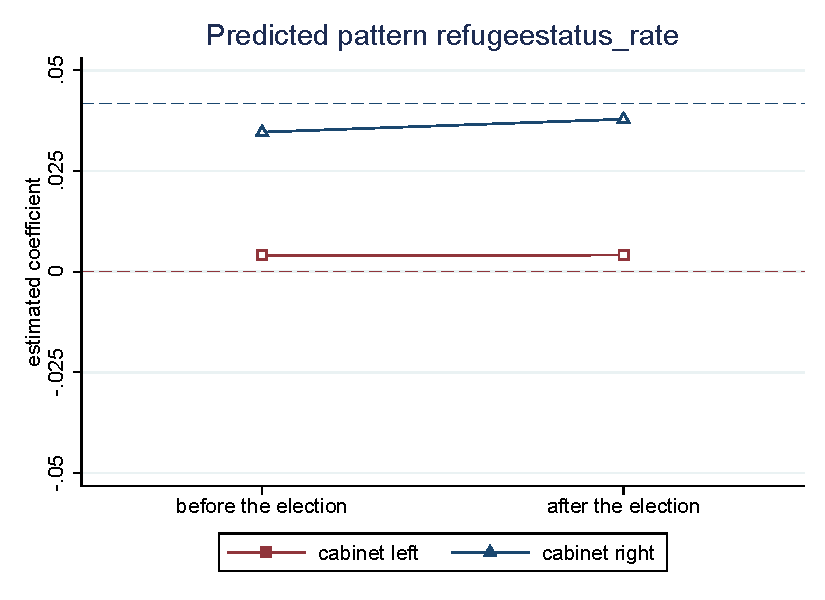
\includegraphics[width=1\textwidth]{figures_edited/refugeestatus_rate_graph1_baseline.pdf}
	\caption{Refugee Status Rate: Predicted Pattern}
\end{figure}

\begin{table}[!ht]\centering
	\renewcommand{\arraystretch}{1.25}
	\def\sym#1{\ifmmode^{#1}\else\(^{#1}\)\fi}
	\caption{Refugee Status Rate: Predicted Pattern}
	\begin{tabular}[]{l*{2}{c}}
		\hline\hline
		                    &\multicolumn{1}{c}{(1)}&\multicolumn{1}{c}{(2)}\\
                    &\multicolumn{1}{c}{left}&\multicolumn{1}{c}{right}\\
\hline
before              &     -0.0147\sym{***}&     0.00575         \\
                    &   (0.00385)         &   (0.00453)         \\
after               &     -0.0139\sym{**} &      0.0100\sym{*}  \\
                    &   (0.00436)         &   (0.00392)         \\
\hline
Observations        &       18224         &       18224         \\

		\hline\hline
		\multicolumn{3}{c}{\footnotesize Standard errors in parentheses} \\
		\multicolumn{3}{c}{\footnotesize (\sym{*} \(p<0.05\), \sym{**} \(p<0.01\), \sym{***} \(p<0.001\))}\\
	\end{tabular}
\end{table}

\clearpage
\textbf{Baseline Specification - Model 2}
\begin{table}[!ht]\centering
	\scriptsize
	\renewcommand{\arraystretch}{1.05}
	\def\sym#1{\ifmmode^{#1}\else\(^{#1}\)\fi}
	\caption{Determinants of refugee status rate}
	\begin{tabular}{l*{3}{c}}
		\hline\hline
		                    &\multicolumn{1}{c}{(1)}         &\multicolumn{1}{c}{(2)}         &\multicolumn{1}{c}{(3)}         \\
\hline
Political Terror Scale&      0.0208\sym{**} &      0.0207\sym{**} &                     \\
                    &   (0.00725)         &   (0.00712)         &                     \\
Civic Liberty (FHI) &      0.0239\sym{*}  &      0.0212         &                     \\
                    &    (0.0107)         &    (0.0109)         &                     \\
Political Rights (FHI)&    -0.00810         &    -0.00613         &                     \\
                    &   (0.00798)         &   (0.00832)         &                     \\
Quarterly civil war battle death (000s)&      0.0110\sym{***}&     0.00981\sym{**} &                     \\
                    &   (0.00282)         &   (0.00284)         &                     \\
Log origin country real GDP per capita&     -0.0204         &     -0.0191         &                     \\
                    &    (0.0191)         &    (0.0203)         &                     \\
Log destination country real GDP per capita&      -0.173\sym{**} &      -0.158\sym{**} &      -0.198\sym{**} \\
                    &    (0.0552)         &    (0.0535)         &    (0.0652)         \\
Quarterly unemployment rate at destination&    -0.00454\sym{***}&    -0.00433\sym{***}&    -0.00525\sym{***}\\
                    &   (0.00121)         &   (0.00115)         &   (0.00139)         \\
Log average past total asylum decisions per capita&     -0.0201\sym{***}&     -0.0262\sym{***}&     -0.0205\sym{***}\\
                    &   (0.00525)         &   (0.00491)         &   (0.00573)         \\
Log average past dyadic asylum decisions per capita&     0.00196         &      0.0103\sym{**} &    -0.00102         \\
                    &   (0.00306)         &   (0.00300)         &   (0.00291)         \\
Cabinet position left * 6 quarters before the election&    -0.00840         &     -0.0111         &    -0.00882         \\
                    &   (0.00858)         &   (0.00872)         &   (0.00864)         \\
Cabinet position left * 5 quarters before the election&     -0.0211\sym{**} &     -0.0202\sym{**} &     -0.0208\sym{**} \\
                    &   (0.00661)         &   (0.00645)         &   (0.00642)         \\
Cabinet position left * 4 quarters before the election&     -0.0301\sym{**} &     -0.0272\sym{**} &     -0.0317\sym{**} \\
                    &   (0.00916)         &   (0.00891)         &   (0.00965)         \\
Cabinet position left * 3 quarters before the election&     -0.0118         &    -0.00957         &     -0.0118         \\
                    &   (0.00869)         &   (0.00857)         &   (0.00857)         \\
Cabinet position left * 2 quarters before the election&     -0.0190\sym{***}&     -0.0171\sym{**} &     -0.0190\sym{***}\\
                    &   (0.00519)         &   (0.00508)         &   (0.00524)         \\
Cabinet position left * 1 quarters before the election&    -0.00657         &    -0.00545         &    -0.00717         \\
                    &   (0.00567)         &   (0.00559)         &   (0.00626)         \\
Cabinet position left * election quarter&    -0.00952         &    -0.00791         &     -0.0112         \\
                    &   (0.00569)         &   (0.00547)         &   (0.00625)         \\
Cabinet position left * 1 quarters after the election&     -0.0200\sym{**} &     -0.0187\sym{**} &     -0.0203\sym{**} \\
                    &   (0.00634)         &   (0.00592)         &   (0.00645)         \\
Cabinet position left * 2 quarters after the election&     -0.0197\sym{**} &     -0.0191\sym{**} &     -0.0194\sym{**} \\
                    &   (0.00709)         &   (0.00699)         &   (0.00711)         \\
Cabinet position left * 3 quarters after the election&    -0.00925         &    -0.00886         &    -0.00957         \\
                    &   (0.00633)         &   (0.00625)         &   (0.00632)         \\
Cabinet position left * 4 quarters after the election&     -0.0106         &     -0.0129         &    -0.00968         \\
                    &   (0.00665)         &   (0.00686)         &   (0.00679)         \\
Cabinet position left * 5 quarters after the election&     -0.0113         &     -0.0134         &     -0.0112         \\
                    &   (0.00701)         &   (0.00738)         &   (0.00736)         \\
Cabinet position left * 6 quarters after the election&    -0.00695         &    -0.00816         &    -0.00831         \\
                    &   (0.00690)         &   (0.00649)         &   (0.00703)         \\
Cabinet position right * 6 quarters before the election&      0.0132\sym{*}  &      0.0128\sym{*}  &     0.00976         \\
                    &   (0.00575)         &   (0.00541)         &   (0.00531)         \\
Cabinet position right * 5 quarters before the election&     0.00843         &      0.0108         &     0.00901         \\
                    &   (0.00708)         &   (0.00676)         &   (0.00765)         \\
Cabinet position right * 4 quarters before the election&    -0.00130         &    0.000531         &    -0.00144         \\
                    &   (0.00891)         &   (0.00865)         &   (0.00937)         \\
Cabinet position right * 3 quarters before the election&     0.00332         &     0.00345         &     0.00571         \\
                    &   (0.00775)         &   (0.00750)         &   (0.00796)         \\
Cabinet position right * 2 quarters before the election&     0.00379         &     0.00428         &     0.00529         \\
                    &   (0.00823)         &   (0.00784)         &   (0.00830)         \\
Cabinet position right * 1 quarters before the election&      0.0164         &      0.0150         &      0.0211\sym{*}  \\
                    &   (0.00865)         &   (0.00845)         &   (0.00893)         \\
Cabinet position right * election quarter&      0.0116         &      0.0128         &      0.0106         \\
                    &   (0.00832)         &   (0.00784)         &   (0.00816)         \\
Cabinet position right * 1 quarters after the election&     0.00424         &     0.00551         &     0.00158         \\
                    &   (0.00706)         &   (0.00714)         &   (0.00734)         \\
Cabinet position right * 2 quarters after the election&     0.00228         &     0.00434         &     0.00163         \\
                    &   (0.00677)         &   (0.00676)         &   (0.00673)         \\
Cabinet position right * 3 quarters after the election&      0.0112         &     0.00879         &      0.0102         \\
                    &   (0.00602)         &   (0.00610)         &   (0.00656)         \\
Cabinet position right * 4 quarters after the election&     0.00768         &     0.00678         &     0.00925         \\
                    &   (0.00541)         &   (0.00520)         &   (0.00561)         \\
Cabinet position right * 5 quarters after the election&      0.0213\sym{**} &      0.0202\sym{*}  &      0.0227\sym{**} \\
                    &   (0.00794)         &   (0.00789)         &   (0.00782)         \\
Cabinet position right * 6 quarters after the election&      0.0126\sym{*}  &      0.0121\sym{*}  &      0.0130\sym{*}  \\
                    &   (0.00590)         &   (0.00543)         &   (0.00579)         \\
\hline
Observations        &       18089         &       18089         &       18089         \\
Adjusted \(R^{2}\)  &       0.133         &       0.060         &       0.117         \\
Fixed Effects       &           O         &       D x O         &       O x T         \\
Destination dummies &         Yes         &          No         &         Yes         \\
Quarter-Year dummies&         Yes         &         Yes         &          No         \\

		\hline\hline
		\multicolumn{4}{c}{\footnotesize Standard errors in parentheses (\sym{*} \(p<0.05\), \sym{**} \(p<0.01\), \sym{***} \(p<0.001\))}\\
	\end{tabular}
\end{table}


\clearpage
\textbf{Baseline Specification - Model 2}
\begin{figure}[!ht]
	\centering
	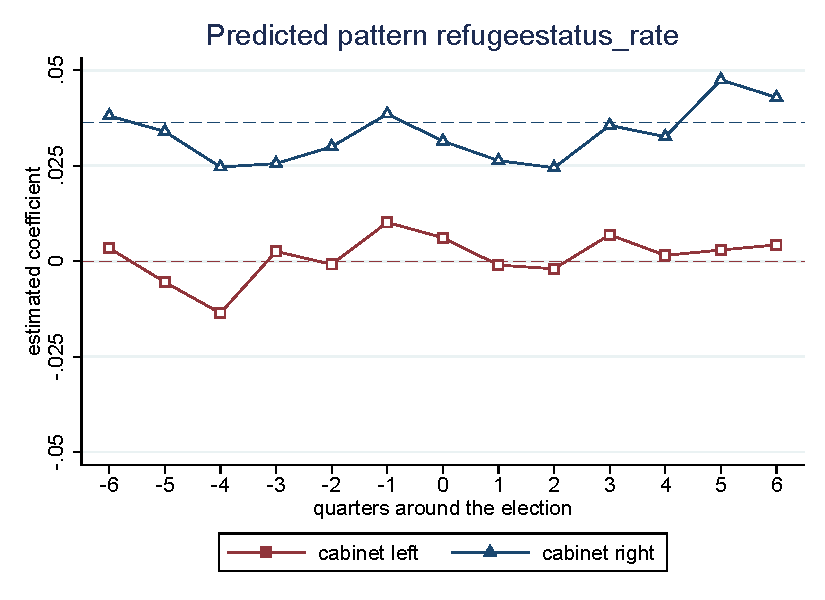
\includegraphics[width=0.7\textwidth]{figures_edited/refugeestatus_rate_graph2_baseline.pdf}
	\caption{Refugee Status Rate: Predicted Pattern}
\end{figure}

\begin{table}[!ht]\centering
	\footnotesize
	\renewcommand{\arraystretch}{1.2}
	\def\sym#1{\ifmmode^{#1}\else\(^{#1}\)\fi}
	\caption{Refugee Status Rate: Predicted Pattern}
	\begin{tabular}{l*{2}{c}}
		\hline\hline
		                    &\multicolumn{1}{c}{(1)}&\multicolumn{1}{c}{(2)}\\
                    &\multicolumn{1}{c}{left}&\multicolumn{1}{c}{right}\\
\hline
 6 quarters before the election&     -0.0111         &      0.0128\sym{*}  \\
                    &   (0.00872)         &   (0.00541)         \\
 5 quarters before the election&     -0.0202\sym{**} &      0.0108         \\
                    &   (0.00645)         &   (0.00676)         \\
 4 quarters before the election&     -0.0272\sym{**} &    0.000531         \\
                    &   (0.00891)         &   (0.00865)         \\
 3 quarters before the election&    -0.00957         &     0.00345         \\
                    &   (0.00857)         &   (0.00750)         \\
 2 quarters before the election&     -0.0171\sym{***}&     0.00428         \\
                    &   (0.00508)         &   (0.00784)         \\
 1 quarters before the election&    -0.00545         &      0.0150         \\
                    &   (0.00559)         &   (0.00845)         \\
Quarter of the election&    -0.00791         &      0.0128         \\
                    &   (0.00547)         &   (0.00784)         \\
 1 quarters after the election&     -0.0187\sym{**} &     0.00551         \\
                    &   (0.00592)         &   (0.00714)         \\
 2 quarters after the election&     -0.0191\sym{**} &     0.00434         \\
                    &   (0.00699)         &   (0.00676)         \\
 3 quarters after the election&    -0.00886         &     0.00879         \\
                    &   (0.00625)         &   (0.00610)         \\
 4 quarters after the election&     -0.0129         &     0.00678         \\
                    &   (0.00686)         &   (0.00520)         \\
 5 quarters after the election&     -0.0134         &      0.0202\sym{*}  \\
                    &   (0.00738)         &   (0.00789)         \\
 6 quarters after the election&    -0.00816         &      0.0121\sym{*}  \\
                    &   (0.00649)         &   (0.00543)         \\
\hline
Observations        &       18089         &       18089         \\

		\hline\hline
		\multicolumn{3}{c}{\footnotesize Standard errors in parentheses} \\
		\multicolumn{3}{c}{\footnotesize (\sym{*} \(p<0.05\), \sym{**} \(p<0.01\), \sym{***} \(p<0.001\))}\\
	\end{tabular}
\end{table}

% ===============================================================================================================


\FloatBarrier
\clearpage
\subsection{Robustness}

\subsubsection{Use destination, origin and time fixed effects}
\textbf{ R1: Use destination, origin and time fixed effects - Model 1}

\begin{figure}[!ht]
	\centering
	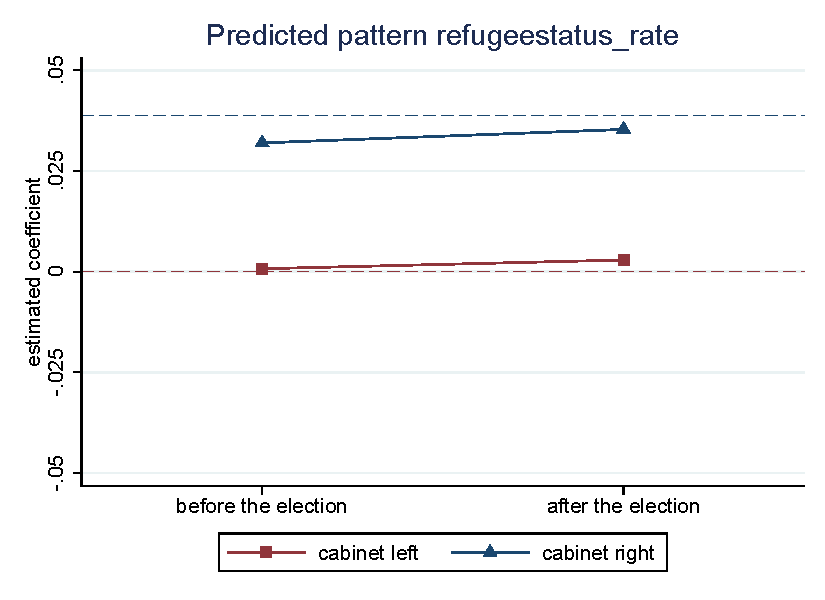
\includegraphics[width=1\textwidth]{figures_edited/refugeestatus_rate_graph1_R1.pdf}
	\caption{R1: Refugee Status Rate: Predicted Pattern}
\end{figure}

\begin{table}[!ht]\centering
	\renewcommand{\arraystretch}{1.25}
	\def\sym#1{\ifmmode^{#1}\else\(^{#1}\)\fi}
	\caption{R1: Refugee Status Rate: Predicted Pattern}
	\begin{tabular}{l*{2}{c}}
		\hline\hline
		                    &\multicolumn{1}{c}{(1)}&\multicolumn{1}{c}{(2)}\\
                    &\multicolumn{1}{c}{left}&\multicolumn{1}{c}{right}\\
\hline
before              &    0.000724         &    -0.00685         \\
                    &   (0.00453)         &   (0.00621)         \\
after               &     0.00290         &    -0.00349         \\
                    &   (0.00358)         &   (0.00390)         \\
\hline
Observations        &       17191         &       17191         \\

		\hline\hline
		\multicolumn{3}{c}{\footnotesize Standard errors in parentheses} \\
		\multicolumn{3}{c}{\footnotesize (\sym{*} \(p<0.05\), \sym{**} \(p<0.01\), \sym{***} \(p<0.001\))}\\
	\end{tabular}
\end{table}

\clearpage
\textbf{ R1: Use destination, origin and time fixed effects - Model 2}
\begin{figure}[!ht]
	\centering
	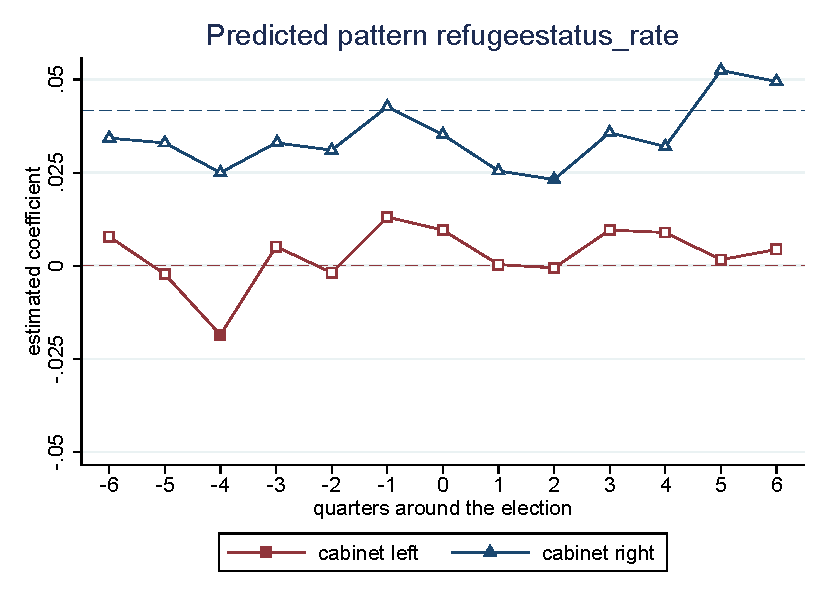
\includegraphics[width=0.7\textwidth]{figures_edited/refugeestatus_rate_graph2_R1.pdf}
	\caption{R1: Refugee Status Rate: Predicted Pattern}
\end{figure}

\begin{table}[!ht]\centering
	\footnotesize
	\renewcommand{\arraystretch}{1.2}
	\def\sym#1{\ifmmode^{#1}\else\(^{#1}\)\fi}
	\caption{R1: Refugee Status Rate: Predicted Pattern}
	\begin{tabular}{l*{2}{c}}
		\hline\hline
		                    &\multicolumn{1}{c}{(1)}&\multicolumn{1}{c}{(2)}\\
                    &\multicolumn{1}{c}{left}&\multicolumn{1}{c}{right}\\
\hline
 6 quarters before the election&     0.00782         &    -0.00747         \\
                    &   (0.00667)         &   (0.00639)         \\
 5 quarters before the election&    -0.00224         &    -0.00877         \\
                    &   (0.00620)         &   (0.00910)         \\
 4 quarters before the election&     -0.0185\sym{*}  &     -0.0167         \\
                    &   (0.00777)         &    (0.0104)         \\
 3 quarters before the election&     0.00516         &    -0.00873         \\
                    &   (0.00966)         &   (0.00976)         \\
 2 quarters before the election&    -0.00184         &     -0.0107         \\
                    &   (0.00614)         &   (0.00804)         \\
 1 quarters before the election&      0.0131         &    0.000911         \\
                    &   (0.00788)         &   (0.00857)         \\
Quarter of the election&     0.00958         &    -0.00654         \\
                    &   (0.00639)         &    (0.0108)         \\
 1 quarters after the election&    0.000343         &     -0.0163         \\
                    &   (0.00700)         &   (0.00904)         \\
 2 quarters after the election&   -0.000576         &     -0.0186\sym{*}  \\
                    &   (0.00521)         &   (0.00811)         \\
 3 quarters after the election&     0.00959         &    -0.00600         \\
                    &   (0.00509)         &   (0.00701)         \\
 4 quarters after the election&     0.00894         &    -0.00975         \\
                    &   (0.00590)         &   (0.00739)         \\
 5 quarters after the election&     0.00164         &      0.0107         \\
                    &   (0.00472)         &   (0.00708)         \\
 6 quarters after the election&     0.00437         &     0.00772         \\
                    &   (0.00672)         &   (0.00592)         \\
\hline
Observations        &       17191         &       17191         \\

		\hline\hline
		\multicolumn{3}{c}{\footnotesize Standard errors in parentheses} \\
		\multicolumn{3}{c}{\footnotesize (\sym{*} \(p<0.05\), \sym{**} \(p<0.01\), \sym{***} \(p<0.001\))}\\
	\end{tabular}
\end{table}

% ===============================================================================================================

\FloatBarrier
\clearpage
\subsubsection{Use destination and origin*time fixed effects}
\textbf{R2: Use destination and origin*time fixed effects - Model 1}

\begin{figure}[!ht]
	\centering
	\includegraphics[width=1\textwidth]{figures_edited/refugeestatus_rate_graph1_R2.pdf}
	\caption{R2: Refugee Status Rate: Predicted Pattern}
\end{figure}

\begin{table}[!ht]\centering
	\renewcommand{\arraystretch}{1.25}
	\def\sym#1{\ifmmode^{#1}\else\(^{#1}\)\fi}
	\caption{R2: Refugee Status Rate: Predicted Pattern}
	\begin{tabular}{l*{2}{c}}
		\hline\hline
		                    &\multicolumn{1}{c}{(1)}&\multicolumn{1}{c}{(2)}\\
                    &\multicolumn{1}{c}{left}&\multicolumn{1}{c}{right}\\
\hline
before              &   -0.000409         &    -0.00590         \\
                    &   (0.00475)         &   (0.00629)         \\
after               &     0.00258         &    -0.00436         \\
                    &   (0.00393)         &   (0.00399)         \\
\hline
Observations        &       17191         &       17191         \\

		\hline\hline
		\multicolumn{3}{c}{\footnotesize Standard errors in parentheses} \\
		\multicolumn{3}{c}{\footnotesize (\sym{*} \(p<0.05\), \sym{**} \(p<0.01\), \sym{***} \(p<0.001\))}\\
	\end{tabular}
\end{table}

\clearpage
\textbf{R2: Use destination and origin*time fixed effects - Model 2}
\begin{figure}[!ht]
	\centering
	\includegraphics[width=0.7\textwidth]{figures_edited/refugeestatus_rate_graph2_R2.pdf}
	\caption{R2: Refugee Status Rate: Predicted Pattern}
\end{figure}

\begin{table}[!ht]\centering
	\footnotesize
	\renewcommand{\arraystretch}{1.2}
	\def\sym#1{\ifmmode^{#1}\else\(^{#1}\)\fi}
	\caption{R2: Refugee Status Rate: Predicted Pattern}
	\begin{tabular}{l*{2}{c}}
		\hline\hline
		                    &\multicolumn{1}{c}{(1)}&\multicolumn{1}{c}{(2)}\\
                    &\multicolumn{1}{c}{left}&\multicolumn{1}{c}{right}\\
\hline
 6 quarters before the election&     0.00768         &     -0.0115         \\
                    &   (0.00685)         &   (0.00662)         \\
 5 quarters before the election&    -0.00223         &    -0.00888         \\
                    &   (0.00592)         &   (0.00955)         \\
 4 quarters before the election&     -0.0225\sym{**} &     -0.0169         \\
                    &   (0.00805)         &    (0.0106)         \\
 3 quarters before the election&     0.00478         &    -0.00863         \\
                    &   (0.00964)         &    (0.0103)         \\
 2 quarters before the election&    -0.00104         &     -0.0129         \\
                    &   (0.00675)         &   (0.00835)         \\
 1 quarters before the election&      0.0120         &     0.00450         \\
                    &   (0.00766)         &   (0.00871)         \\
Quarter of the election&     0.00675         &    -0.00730         \\
                    &   (0.00667)         &    (0.0105)         \\
 1 quarters after the election&    0.000292         &     -0.0187         \\
                    &   (0.00712)         &   (0.00961)         \\
 2 quarters after the election&   -0.000904         &     -0.0218\sym{*}  \\
                    &   (0.00557)         &   (0.00855)         \\
 3 quarters after the election&     0.00914         &    -0.00847         \\
                    &   (0.00546)         &   (0.00715)         \\
 4 quarters after the election&     0.00936         &     -0.0103         \\
                    &   (0.00607)         &   (0.00760)         \\
 5 quarters after the election&     0.00136         &      0.0101         \\
                    &   (0.00537)         &   (0.00679)         \\
 6 quarters after the election&     0.00211         &     0.00647         \\
                    &   (0.00710)         &   (0.00594)         \\
\hline
Observations        &       17191         &       17191         \\

		\hline\hline
		\multicolumn{3}{c}{\footnotesize Standard errors in parentheses} \\
		\multicolumn{3}{c}{\footnotesize (\sym{*} \(p<0.05\), \sym{**} \(p<0.01\), \sym{***} \(p<0.001\))}\\
	\end{tabular}
\end{table}


% ===============================================================================================================


\clearpage
\FloatBarrier
\subsubsection{Control for past asylum applications}
\begin{table}[!ht]\centering
	\renewcommand{\arraystretch}{1.25}
	\small
	\def\sym#1{\ifmmode^{#1}\else\(^{#1}\)\fi}
	\caption{R3: Determinants of refugee status rate}
	\begin{tabular}{l*{3}{c}}
		\hline\hline
		                                        &\multicolumn{1}{c}{(1)}         &\multicolumn{1}{c}{(2)}         &\multicolumn{1}{c}{(3)}         \\
\hline
Political Terror Scale                  &    0.0198\sym{*}  &    0.0231\sym{**} &                   \\
                                        & (0.00779)         & (0.00810)         &                   \\
Civic Liberty (FHI)                     &    0.0239\sym{*}  &    0.0211         &                   \\
                                        &  (0.0116)         &  (0.0123)         &                   \\
Political Rights (FHI)                  &  -0.00825         &  -0.00650         &                   \\
                                        & (0.00788)         & (0.00860)         &                   \\
Quarterly civil war battle death (000s) &    0.0145\sym{***}&    0.0153\sym{***}&                   \\
                                        & (0.00360)         & (0.00394)         &                   \\
Log origin country real GDP per capita  &   -0.0149         &   -0.0175         &                   \\
                                        &  (0.0258)         &  (0.0273)         &                   \\
Log migrant stock in 2000/1             &  -0.00337         &                   &  -0.00304         \\
                                        & (0.00234)         &                   & (0.00240)         \\
Log distance from origin to destination &    0.0166         &                   &    0.0159         \\
                                        &  (0.0143)         &                   &  (0.0144)         \\
Log destination country real GDP per capita&    -0.161\sym{**} &    -0.157\sym{**} &    -0.154\sym{**} \\
                                        &  (0.0585)         &  (0.0565)         &  (0.0567)         \\
Quarterly unemployment rate at destination&  -0.00426\sym{**} &  -0.00417\sym{**} &  -0.00447\sym{**} \\
                                        & (0.00132)         & (0.00124)         & (0.00136)         \\
Log average past total asylum decisions per capita&    -165.0\sym{***}&    -167.5\sym{***}&    -164.5\sym{***}\\
                                        &   (38.59)         &   (34.96)         &   (38.82)         \\
Log average past dyadic asylum decisions per capita&    -206.9         &    -191.4         &    -371.4         \\
                                        &   (212.3)         &   (142.8)         &   (226.7)         \\
Log average past asylum applications at destination per capita&    0.0244\sym{**} &    0.0230\sym{**} &    0.0238\sym{**} \\
                                        & (0.00828)         & (0.00786)         & (0.00866)         \\
Weighted cabinet position right         &    0.0394\sym{***}&    0.0420\sym{***}&    0.0394\sym{***}\\
                                        &  (0.0100)         & (0.00994)         &  (0.0100)         \\
Cabinet position left * Before the election&   0.00180         &   0.00456         &  0.000736         \\
                                        & (0.00448)         & (0.00447)         & (0.00466)         \\
Cabinet position left * After the election&  0.000674         &   0.00178         &  0.000340         \\
                                        & (0.00377)         & (0.00369)         & (0.00414)         \\
Cabinet position right * Before the election&  -0.00768         &  -0.00757         &  -0.00684         \\
                                        & (0.00622)         & (0.00586)         & (0.00628)         \\
Cabinet position right * After the election&  -0.00376         &  -0.00427         &  -0.00462         \\
                                        & (0.00390)         & (0.00371)         & (0.00399)         \\
\hline
Observations                            &     17136         &     17136         &     17136         \\
Adjusted \(R^{2}\)                      &     0.145         &     0.069         &     0.131         \\
Fixed Effects                           &         O         &     D x O         &     O x T         \\
Destination dummies                     &       Yes         &        No         &       Yes         \\
Quarter-Year dummies                    &       Yes         &       Yes         &        No         \\

		\hline\hline
		\multicolumn{4}{l}{\footnotesize Standard errors in parentheses (\sym{*} \(p<0.05\), \sym{**} \(p<0.01\), \sym{***} \(p<0.001\))}\\
	\end{tabular}
\end{table}

\clearpage
\textbf{R3: Control for past asylum applications - Model 1}
\begin{figure}[!ht]
	\centering
	\includegraphics[width=1\textwidth]{figures_edited/refugeestatus_rate_graph1_R3.pdf}
	\caption{R3: Refugee Status Rate: Predicted Pattern}
\end{figure}

\begin{table}[!ht]\centering
	\renewcommand{\arraystretch}{1.25}
	\def\sym#1{\ifmmode^{#1}\else\(^{#1}\)\fi}
	\caption{R3: Refugee Status Rate: Predicted Pattern}
	\begin{tabular}{l*{2}{c}}
		\hline\hline
		                    &\multicolumn{1}{c}{(1)}&\multicolumn{1}{c}{(2)}\\
                    &\multicolumn{1}{c}{left}&\multicolumn{1}{c}{right}\\
\hline
before              &     0.00456         &    -0.00757         \\
                    &   (0.00447)         &   (0.00586)         \\
after               &     0.00178         &    -0.00427         \\
                    &   (0.00369)         &   (0.00371)         \\
\hline
Observations        &       17136         &       17136         \\

		\hline\hline
		\multicolumn{3}{c}{\footnotesize Standard errors in parentheses} \\
		\multicolumn{3}{c}{\footnotesize (\sym{*} \(p<0.05\), \sym{**} \(p<0.01\), \sym{***} \(p<0.001\))}\\
	\end{tabular}
\end{table}

\clearpage
\textbf{R3: Control for past asylum applications - Model 2}
\begin{figure}[!ht]
	\centering
	\includegraphics[width=0.7\textwidth]{figures_edited/refugeestatus_rate_graph2_R3.pdf}
	\caption{R3: Refugee Status Rate: Predicted Pattern}
\end{figure}

\begin{table}[!ht]\centering
	\footnotesize
	\renewcommand{\arraystretch}{1.2}
	\def\sym#1{\ifmmode^{#1}\else\(^{#1}\)\fi}
	\caption{R3: Refugee Status Rate: Predicted Pattern}
	\begin{tabular}{l*{2}{c}}
		\hline\hline
		                    &\multicolumn{1}{c}{(1)}&\multicolumn{1}{c}{(2)}\\
                    &\multicolumn{1}{c}{left}&\multicolumn{1}{c}{right}\\
\hline
 6 quarters before the election&      0.0106         &     -0.0103         \\
                    &   (0.00632)         &   (0.00654)         \\
 5 quarters before the election&     0.00580         &    -0.00907         \\
                    &   (0.00621)         &   (0.00887)         \\
 4 quarters before the election&     -0.0116         &     -0.0155         \\
                    &   (0.00704)         &   (0.00993)         \\
 3 quarters before the election&      0.0105         &     -0.0125         \\
                    &   (0.00931)         &    (0.0100)         \\
 2 quarters before the election&   -0.000361         &     -0.0121         \\
                    &   (0.00644)         &   (0.00751)         \\
 1 quarters before the election&      0.0165\sym{*}  &    0.000502         \\
                    &   (0.00803)         &   (0.00842)         \\
Quarter of the election&      0.0125         &     -0.0104         \\
                    &   (0.00653)         &   (0.00987)         \\
 1 quarters after the election&     0.00217         &     -0.0146         \\
                    &   (0.00736)         &   (0.00869)         \\
 2 quarters after the election&    0.000710         &     -0.0182\sym{*}  \\
                    &   (0.00589)         &   (0.00806)         \\
 3 quarters after the election&     0.00955         &    -0.00946         \\
                    &   (0.00551)         &   (0.00695)         \\
 4 quarters after the election&     0.00500         &     -0.0139         \\
                    &   (0.00609)         &   (0.00727)         \\
 5 quarters after the election&     0.00134         &     0.00769         \\
                    &   (0.00439)         &   (0.00741)         \\
 6 quarters after the election&     0.00220         &     0.00779         \\
                    &   (0.00669)         &   (0.00536)         \\
\hline
Observations        &       17136         &       17136         \\

		\hline\hline
		\multicolumn{3}{c}{\footnotesize Standard errors in parentheses} \\
		\multicolumn{3}{c}{\footnotesize (\sym{*} \(p<0.05\), \sym{**} \(p<0.01\), \sym{***} \(p<0.001\))} \\
	\end{tabular}
\end{table}


% ===============================================================================================================


\clearpage
\FloatBarrier
\subsubsection{Include cabinet right dummy}
\begin{table}[!ht]\centering
	\renewcommand{\arraystretch}{1.25}
	\small
	\def\sym#1{\ifmmode^{#1}\else\(^{#1}\)\fi}
	\caption{R4: Determinants of refugee status rate}
	\begin{tabular}{l*{3}{c}}
		\hline\hline
		                                        &\multicolumn{1}{c}{(1)}         &\multicolumn{1}{c}{(2)}         &\multicolumn{1}{c}{(3)}         \\
\hline
Political Terror Scale                  &    0.0206\sym{*}  &    0.0238\sym{**} &                   \\
                                        & (0.00777)         & (0.00804)         &                   \\
Civic Liberty (FHI)                     &    0.0239\sym{*}  &    0.0209         &                   \\
                                        &  (0.0116)         &  (0.0123)         &                   \\
Political Rights (FHI)                  &  -0.00855         &  -0.00663         &                   \\
                                        & (0.00803)         & (0.00884)         &                   \\
Quarterly civil war battle death (000s) &    0.0144\sym{***}&    0.0152\sym{***}&                   \\
                                        & (0.00357)         & (0.00388)         &                   \\
Log origin country real GDP per capita  &   -0.0146         &   -0.0177         &                   \\
                                        &  (0.0257)         &  (0.0272)         &                   \\
Log migrant stock in 2000/1             &  -0.00317         &                   &  -0.00283         \\
                                        & (0.00234)         &                   & (0.00240)         \\
Log distance from origin to destination &    0.0178         &                   &    0.0170         \\
                                        &  (0.0143)         &                   &  (0.0143)         \\
Log destination country real GDP per capita&    -0.171\sym{**} &    -0.160\sym{**} &    -0.167\sym{**} \\
                                        &  (0.0563)         &  (0.0543)         &  (0.0559)         \\
Quarterly unemployment rate at destination&  -0.00443\sym{**} &  -0.00426\sym{**} &  -0.00469\sym{**} \\
                                        & (0.00132)         & (0.00124)         & (0.00137)         \\
Log average past total asylum decisions per capita&    -122.9\sym{***}&    -128.4\sym{***}&    -123.1\sym{***}\\
                                        &   (28.99)         &   (26.67)         &   (29.20)         \\
Log average past dyadic asylum decisions per capita&    -204.3         &    -193.0         &    -371.9         \\
                                        &   (214.0)         &   (151.5)         &   (227.3)         \\
Cabinet position left * Before the election&   -0.0195\sym{***}&   -0.0177\sym{***}&   -0.0207\sym{***}\\
                                        & (0.00441)         & (0.00415)         & (0.00467)         \\
Cabinet position left * After the election&   -0.0166\sym{***}&   -0.0167\sym{***}&   -0.0169\sym{***}\\
                                        & (0.00448)         & (0.00442)         & (0.00455)         \\
Cabinet position right * Before the election&    0.0113\sym{*}  &    0.0121\sym{*}  &    0.0122\sym{*}  \\
                                        & (0.00557)         & (0.00526)         & (0.00586)         \\
Cabinet position right * After the election&    0.0158\sym{***}&    0.0161\sym{***}&    0.0148\sym{***}\\
                                        & (0.00392)         & (0.00386)         & (0.00365)         \\
\hline
Observations                            &     17191         &     17191         &     17191         \\
Adjusted \(R^{2}\)                      &     0.140         &     0.062         &     0.126         \\
Fixed Effects                           &         O         &     D x O         &     O x T         \\
Destination dummies                     &       Yes         &        No         &       Yes         \\
Quarter-Year dummies                    &       Yes         &       Yes         &        No         \\

		\hline\hline
		\multicolumn{4}{l}{\footnotesize Standard errors in parentheses (\sym{*} \(p<0.05\), \sym{**} \(p<0.01\), \sym{***} \(p<0.001\))}\\
	\end{tabular}
\end{table}

\clearpage
\textbf{R4: Include cabinet right dummy - Model 1}
\begin{figure}[!ht]
	\centering
	\includegraphics[width=1\textwidth]{figures_edited/refugeestatus_rate_graph1_R4.pdf}
	\caption{R4: Refugee Status Rate: Predicted Pattern}
\end{figure}

\begin{table}[!ht]\centering
	\renewcommand{\arraystretch}{1.25}
	\def\sym#1{\ifmmode^{#1}\else\(^{#1}\)\fi}
	\caption{R4: Refugee Status Rate: Predicted Pattern}
	\begin{tabular}{l*{2}{c}}
		\hline\hline
		                    &\multicolumn{1}{c}{(1)}&\multicolumn{1}{c}{(2)}\\
                    &\multicolumn{1}{c}{left}&\multicolumn{1}{c}{right}\\
\hline
before              &     -0.0177\sym{***}&      0.0121\sym{*}  \\
                    &   (0.00415)         &   (0.00526)         \\
after               &     -0.0167\sym{***}&      0.0161\sym{***}\\
                    &   (0.00442)         &   (0.00386)         \\
\hline
Observations        &       17191         &       17191         \\

		\hline\hline
		\multicolumn{3}{c}{\footnotesize Standard errors in parentheses} \\
		\multicolumn{3}{c}{\footnotesize (\sym{*} \(p<0.05\), \sym{**} \(p<0.01\), \sym{***} \(p<0.001\))}\\
	\end{tabular}
\end{table}

\clearpage
\textbf{R4: Include cabinet right dummy - Model 2}
\begin{figure}[!ht]
	\centering
	\includegraphics[width=0.7\textwidth]{figures_edited/refugeestatus_rate_graph2_R4.pdf}
	\caption{R4: Refugee Status Rate: Predicted Pattern}
\end{figure}

\begin{table}[!ht]\centering
	\footnotesize
	\renewcommand{\arraystretch}{1.2}
	\def\sym#1{\ifmmode^{#1}\else\(^{#1}\)\fi}
	\caption{R4: Refugee Status Rate: Predicted Pattern}
	\begin{tabular}{l*{2}{c}}
		\hline\hline
		                    &\multicolumn{1}{c}{(1)}&\multicolumn{1}{c}{(2)}\\
                    &\multicolumn{1}{c}{left}&\multicolumn{1}{c}{right}\\
\hline
 6 quarters before the election&     -0.0151         &      0.0114\sym{*}  \\
                    &   (0.00857)         &   (0.00568)         \\
 5 quarters before the election&     -0.0204\sym{**} &      0.0124         \\
                    &   (0.00734)         &   (0.00793)         \\
 4 quarters before the election&     -0.0365\sym{***}&     0.00587         \\
                    &   (0.00914)         &   (0.00923)         \\
 3 quarters before the election&     -0.0141         &     0.00903         \\
                    &   (0.00881)         &   (0.00794)         \\
 2 quarters before the election&     -0.0218\sym{**} &      0.0115         \\
                    &   (0.00664)         &   (0.00870)         \\
 1 quarters before the election&    -0.00864         &      0.0208\sym{*}  \\
                    &   (0.00646)         &   (0.00847)         \\
Quarter of the election&     -0.0118\sym{*}  &      0.0131         \\
                    &   (0.00529)         &   (0.00789)         \\
 1 quarters after the election&     -0.0190\sym{**} &     0.00671         \\
                    &   (0.00623)         &   (0.00724)         \\
 2 quarters after the election&     -0.0202\sym{**} &     0.00557         \\
                    &   (0.00621)         &   (0.00587)         \\
 3 quarters after the election&     -0.0101         &      0.0143\sym{*}  \\
                    &   (0.00604)         &   (0.00653)         \\
 4 quarters after the election&     -0.0155\sym{*}  &     0.00902         \\
                    &   (0.00758)         &   (0.00513)         \\
 5 quarters after the election&     -0.0187\sym{**} &      0.0297\sym{**} \\
                    &   (0.00633)         &   (0.00945)         \\
 6 quarters after the election&     -0.0194\sym{**} &      0.0288\sym{***}\\
                    &   (0.00730)         &   (0.00633)         \\
\hline
Observations        &       17191         &       17191         \\

		\hline\hline
		\multicolumn{3}{c}{\footnotesize Standard errors in parentheses} \\
		\multicolumn{3}{c}{\footnotesize (\sym{*} \(p<0.05\), \sym{**} \(p<0.01\), \sym{***} \(p<0.001\))} \\
	\end{tabular}
\end{table}


% ===============================================================================================================



\clearpage
\FloatBarrier
\subsubsection{Do not use lags for origin country variables}
\begin{table}[!ht]\centering
	\renewcommand{\arraystretch}{1.25}
	\small
	\def\sym#1{\ifmmode^{#1}\else\(^{#1}\)\fi}
	\caption{R5: Determinants of refugee status rate}
	\begin{tabular}{l*{3}{c}}
		\hline\hline
		                                        &\multicolumn{1}{c}{(1)}         &\multicolumn{1}{c}{(2)}         &\multicolumn{1}{c}{(3)}         \\
\hline
Political Terror Scale                  &    0.0159\sym{*}  &    0.0190\sym{**} &                   \\
                                        & (0.00641)         & (0.00676)         &                   \\
Civic Liberty (FHI)                     &    0.0208         &    0.0188         &                   \\
                                        &  (0.0106)         &  (0.0112)         &                   \\
Political Rights (FHI)                  &  -0.00778         &  -0.00640         &                   \\
                                        & (0.00740)         & (0.00798)         &                   \\
Quarterly civil war battle death (000s) &    0.0116\sym{***}&    0.0118\sym{***}&                   \\
                                        & (0.00311)         & (0.00333)         &                   \\
Log origin country real GDP per capita  &   -0.0211         &   -0.0243         &                   \\
                                        &  (0.0273)         &  (0.0286)         &                   \\
Log migrant stock in 2000/1             &  -0.00335         &                   &  -0.00293         \\
                                        & (0.00234)         &                   & (0.00240)         \\
Log distance from origin to destination &    0.0175         &                   &    0.0170         \\
                                        &  (0.0142)         &                   &  (0.0143)         \\
Log destination country real GDP per capita&    -0.175\sym{**} &    -0.165\sym{**} &    -0.172\sym{**} \\
                                        &  (0.0568)         &  (0.0548)         &  (0.0561)         \\
Quarterly unemployment rate at destination&  -0.00420\sym{**} &  -0.00402\sym{**} &  -0.00446\sym{**} \\
                                        & (0.00129)         & (0.00120)         & (0.00134)         \\
Log average past total asylum decisions per capita&    -123.2\sym{***}&    -129.8\sym{***}&    -121.6\sym{***}\\
                                        &   (29.46)         &   (27.33)         &   (29.17)         \\
Log average past dyadic asylum decisions per capita&    -159.9         &    -107.4         &    -372.3         \\
                                        &   (217.3)         &   (134.1)         &   (227.9)         \\
Weighted cabinet position right         &    0.0396\sym{***}&    0.0420\sym{***}&    0.0394\sym{***}\\
                                        &  (0.0101)         &  (0.0100)         &  (0.0101)         \\
Cabinet position left * Before the election&   0.00135         &   0.00432         &-0.0000109         \\
                                        & (0.00459)         & (0.00455)         & (0.00477)         \\
Cabinet position left * After the election&   0.00315         &   0.00418         &   0.00276         \\
                                        & (0.00358)         & (0.00357)         & (0.00391)         \\
Cabinet position right * Before the election&  -0.00695         &  -0.00719         &  -0.00605         \\
                                        & (0.00627)         & (0.00591)         & (0.00628)         \\
Cabinet position right * After the election&  -0.00327         &  -0.00390         &  -0.00423         \\
                                        & (0.00391)         & (0.00371)         & (0.00400)         \\
\hline
Observations                            &     17191         &     17191         &     17191         \\
Adjusted \(R^{2}\)                      &     0.141         &     0.064         &     0.129         \\
Fixed Effects                           &         O         &     D x O         &     O x T         \\
Destination dummies                     &       Yes         &        No         &       Yes         \\
Quarter-Year dummies                    &       Yes         &       Yes         &        No         \\

		\hline\hline
		\multicolumn{4}{l}{\footnotesize Standard errors in parentheses (\sym{*} \(p<0.05\), \sym{**} \(p<0.01\), \sym{***} \(p<0.001\))}\\
	\end{tabular}
\end{table}

\clearpage
\textbf{R5: Do not use lags for origin country variables - Model 1}
\begin{figure}[!ht]
	\centering
	\includegraphics[width=1\textwidth]{figures_edited/refugeestatus_rate_graph1_R5.pdf}
	\caption{R5: Refugee Status Rate: Predicted Pattern}
\end{figure}

\begin{table}[!ht]\centering
	\renewcommand{\arraystretch}{1.25}
	\def\sym#1{\ifmmode^{#1}\else\(^{#1}\)\fi}
	\caption{R5: Refugee Status Rate: Predicted Pattern}
	\begin{tabular}{l*{2}{c}}
		\hline\hline
		                    &\multicolumn{1}{c}{(1)}&\multicolumn{1}{c}{(2)}\\
                    &\multicolumn{1}{c}{left}&\multicolumn{1}{c}{right}\\
\hline
before              &     0.00432         &    -0.00719         \\
                    &   (0.00455)         &   (0.00591)         \\
after               &     0.00418         &    -0.00390         \\
                    &   (0.00357)         &   (0.00371)         \\
\hline
Observations        &       17191         &       17191         \\

		\hline\hline
		\multicolumn{3}{c}{\footnotesize Standard errors in parentheses} \\
		\multicolumn{3}{c}{\footnotesize (\sym{*} \(p<0.05\), \sym{**} \(p<0.01\), \sym{***} \(p<0.001\))}\\
	\end{tabular}
\end{table}

\clearpage
\textbf{R5: Do not use lags for origin country variables - Model 2}
\begin{figure}[!ht]
	\centering
	\includegraphics[width=0.7\textwidth]{figures_edited/refugeestatus_rate_graph2_R5.pdf}
	\caption{R5: Refugee Status Rate: Predicted Pattern}
\end{figure}

\begin{table}[!ht]\centering
	\footnotesize
	\renewcommand{\arraystretch}{1.2}
	\def\sym#1{\ifmmode^{#1}\else\(^{#1}\)\fi}
	\caption{R5: Refugee Status Rate: Predicted Pattern}
	\begin{tabular}{l*{2}{c}}
		\hline\hline
		                    &\multicolumn{1}{c}{(1)}&\multicolumn{1}{c}{(2)}\\
                    &\multicolumn{1}{c}{left}&\multicolumn{1}{c}{right}\\
\hline
 6 quarters before the election&     0.00904         &    -0.00930         \\
                    &   (0.00642)         &   (0.00657)         \\
 5 quarters before the election&     0.00382         &    -0.00834         \\
                    &   (0.00615)         &   (0.00892)         \\
 4 quarters before the election&     -0.0125         &     -0.0151         \\
                    &   (0.00716)         &   (0.00988)         \\
 3 quarters before the election&     0.00912         &     -0.0121         \\
                    &   (0.00938)         &    (0.0100)         \\
 2 quarters before the election&     0.00121         &     -0.0106         \\
                    &   (0.00653)         &   (0.00753)         \\
 1 quarters before the election&      0.0159\sym{*}  &   -0.000877         \\
                    &   (0.00792)         &   (0.00807)         \\
Quarter of the election&      0.0123         &    -0.00844         \\
                    &   (0.00646)         &    (0.0103)         \\
 1 quarters after the election&     0.00420         &     -0.0152         \\
                    &   (0.00714)         &   (0.00869)         \\
 2 quarters after the election&     0.00183         &     -0.0165\sym{*}  \\
                    &   (0.00589)         &   (0.00792)         \\
 3 quarters after the election&      0.0121\sym{*}  &    -0.00825         \\
                    &   (0.00527)         &   (0.00683)         \\
 4 quarters after the election&     0.00717         &     -0.0132         \\
                    &   (0.00610)         &   (0.00728)         \\
 5 quarters after the election&     0.00393         &     0.00794         \\
                    &   (0.00439)         &   (0.00741)         \\
 6 quarters after the election&     0.00451         &     0.00824         \\
                    &   (0.00650)         &   (0.00543)         \\
\hline
Observations        &       17191         &       17191         \\

		\hline\hline
		\multicolumn{3}{c}{\footnotesize Standard errors in parentheses} \\
		\multicolumn{3}{c}{\footnotesize (\sym{*} \(p<0.05\), \sym{**} \(p<0.01\), \sym{***} \(p<0.001\))} \\
	\end{tabular}
\end{table}


% ===============================================================================================================


\clearpage
\FloatBarrier
\subsubsection{Use Syrian battle death data from UCDP}
\begin{table}[!ht]\centering
	\renewcommand{\arraystretch}{1.25}
	\small
	\def\sym#1{\ifmmode^{#1}\else\(^{#1}\)\fi}
	\caption{R6: Determinants of refugee status rate}
	\begin{tabular}{l*{3}{c}}
		\hline\hline
		                                        &\multicolumn{1}{c}{(1)}         &\multicolumn{1}{c}{(2)}         &\multicolumn{1}{c}{(3)}         \\
\hline
Political Terror Scale                  &    0.0197\sym{*}  &    0.0229\sym{**} &                   \\
                                        & (0.00744)         & (0.00769)         &                   \\
Civic Liberty (FHI)                     &    0.0237\sym{*}  &    0.0206         &                   \\
                                        &  (0.0112)         &  (0.0120)         &                   \\
Political Rights (FHI)                  &  -0.00850         &  -0.00649         &                   \\
                                        & (0.00777)         & (0.00852)         &                   \\
Quarterly civil war battle death (000s) &    0.0114\sym{***}&    0.0122\sym{***}&                   \\
                                        & (0.00201)         & (0.00221)         &                   \\
Log origin country real GDP per capita  &   -0.0127         &   -0.0159         &                   \\
                                        &  (0.0261)         &  (0.0274)         &                   \\
Log migrant stock in 2000/1             &  -0.00319         &                   &  -0.00293         \\
                                        & (0.00234)         &                   & (0.00240)         \\
Log distance from origin to destination &    0.0177         &                   &    0.0170         \\
                                        &  (0.0142)         &                   &  (0.0143)         \\
Log destination country real GDP per capita&    -0.179\sym{**} &    -0.167\sym{**} &    -0.172\sym{**} \\
                                        &  (0.0569)         &  (0.0546)         &  (0.0561)         \\
Quarterly unemployment rate at destination&  -0.00424\sym{**} &  -0.00406\sym{**} &  -0.00446\sym{**} \\
                                        & (0.00130)         & (0.00121)         & (0.00134)         \\
Log average past total asylum decisions per capita&    -119.6\sym{***}&    -124.2\sym{***}&    -121.6\sym{***}\\
                                        &   (28.31)         &   (26.11)         &   (29.17)         \\
Log average past dyadic asylum decisions per capita&    -248.7         &    -277.3         &    -372.3         \\
                                        &   (216.5)         &   (177.5)         &   (227.9)         \\
Weighted cabinet position right         &    0.0393\sym{***}&    0.0418\sym{***}&    0.0394\sym{***}\\
                                        &  (0.0101)         &  (0.0100)         &  (0.0101)         \\
Cabinet position left * Before the election&   0.00101         &   0.00393         &-0.0000109         \\
                                        & (0.00462)         & (0.00456)         & (0.00477)         \\
Cabinet position left * After the election&   0.00309         &   0.00410         &   0.00276         \\
                                        & (0.00358)         & (0.00357)         & (0.00391)         \\
Cabinet position right * Before the election&  -0.00697         &  -0.00722         &  -0.00605         \\
                                        & (0.00621)         & (0.00584)         & (0.00628)         \\
Cabinet position right * After the election&  -0.00329         &  -0.00393         &  -0.00423         \\
                                        & (0.00391)         & (0.00371)         & (0.00400)         \\
\hline
Observations                            &     17191         &     17191         &     17191         \\
Adjusted \(R^{2}\)                      &     0.145         &     0.069         &     0.129         \\
Fixed Effects                           &         O         &     D x O         &     O x T         \\
Destination dummies                     &       Yes         &        No         &       Yes         \\
Quarter-Year dummies                    &       Yes         &       Yes         &        No         \\

		\hline\hline
		\multicolumn{4}{l}{\footnotesize Standard errors in parentheses (\sym{*} \(p<0.05\), \sym{**} \(p<0.01\), \sym{***} \(p<0.001\))}\\
	\end{tabular}
\end{table}

\clearpage
\textbf{R6: Use Syrian battle death data from UCDP - Model 1}
\begin{figure}[!ht]
	\centering
	\includegraphics[width=1\textwidth]{figures_edited/refugeestatus_rate_graph1_R6.pdf}
	\caption{R6: Refugee Status Rate: Predicted Pattern}
\end{figure}

\begin{table}[!ht]\centering
	\renewcommand{\arraystretch}{1.25}
	\def\sym#1{\ifmmode^{#1}\else\(^{#1}\)\fi}
	\caption{R6: Refugee Status Rate: Predicted Pattern}
	\begin{tabular}{l*{2}{c}}
		\hline\hline
		                    &\multicolumn{1}{c}{(1)}&\multicolumn{1}{c}{(2)}\\
                    &\multicolumn{1}{c}{left}&\multicolumn{1}{c}{right}\\
\hline
before              &     0.00393         &    -0.00722         \\
                    &   (0.00456)         &   (0.00584)         \\
after               &     0.00410         &    -0.00393         \\
                    &   (0.00357)         &   (0.00371)         \\
\hline
Observations        &       17191         &       17191         \\

		\hline\hline
		\multicolumn{3}{c}{\footnotesize Standard errors in parentheses} \\
		\multicolumn{3}{c}{\footnotesize (\sym{*} \(p<0.05\), \sym{**} \(p<0.01\), \sym{***} \(p<0.001\))}\\
	\end{tabular}
\end{table}

\clearpage
\textbf{R6: Use Syrian battle death data from UCDP - Model 2}
\begin{figure}[!ht]
	\centering
	\includegraphics[width=0.7\textwidth]{figures_edited/refugeestatus_rate_graph2_R6.pdf}
	\caption{R6: Refugee Status Rate: Predicted Pattern}
\end{figure}

\begin{table}[!ht]\centering
	\footnotesize
	\renewcommand{\arraystretch}{1.2}
	\def\sym#1{\ifmmode^{#1}\else\(^{#1}\)\fi}
	\caption{R6: Refugee Status Rate: Predicted Pattern}
	\begin{tabular}{l*{2}{c}}
		\hline\hline
		                    &\multicolumn{1}{c}{(1)}&\multicolumn{1}{c}{(2)}\\
                    &\multicolumn{1}{c}{left}&\multicolumn{1}{c}{right}\\
\hline
 6 quarters before the election&     0.00907         &    -0.00925         \\
                    &   (0.00644)         &   (0.00651)         \\
 5 quarters before the election&     0.00328         &    -0.00835         \\
                    &   (0.00619)         &   (0.00885)         \\
 4 quarters before the election&     -0.0132         &     -0.0154         \\
                    &   (0.00721)         &   (0.00984)         \\
 3 quarters before the election&     0.00857         &     -0.0121         \\
                    &   (0.00936)         &   (0.01000)         \\
 2 quarters before the election&    0.000735         &     -0.0103         \\
                    &   (0.00659)         &   (0.00745)         \\
 1 quarters before the election&      0.0158\sym{*}  &   -0.000780         \\
                    &   (0.00792)         &   (0.00801)         \\
Quarter of the election&      0.0121         &    -0.00854         \\
                    &   (0.00650)         &    (0.0103)         \\
 1 quarters after the election&     0.00401         &     -0.0151         \\
                    &   (0.00719)         &   (0.00868)         \\
 2 quarters after the election&     0.00178         &     -0.0165\sym{*}  \\
                    &   (0.00590)         &   (0.00790)         \\
 3 quarters after the election&      0.0119\sym{*}  &    -0.00820         \\
                    &   (0.00527)         &   (0.00681)         \\
 4 quarters after the election&     0.00700         &     -0.0133         \\
                    &   (0.00608)         &   (0.00721)         \\
 5 quarters after the election&     0.00401         &     0.00783         \\
                    &   (0.00435)         &   (0.00739)         \\
 6 quarters after the election&     0.00455         &     0.00816         \\
                    &   (0.00647)         &   (0.00548)         \\
\hline
Observations        &       17191         &       17191         \\

		\hline\hline
		\multicolumn{3}{c}{\footnotesize Standard errors in parentheses} \\
		\multicolumn{3}{c}{\footnotesize (\sym{*} \(p<0.05\), \sym{**} \(p<0.01\), \sym{***} \(p<0.001\))} \\
	\end{tabular}
\end{table}


% ===============================================================================================================


\clearpage
\FloatBarrier
\subsubsection{Include a post 2007 dummy}
\begin{table}[!ht]\centering
	\renewcommand{\arraystretch}{1.25}
	\small
	\def\sym#1{\ifmmode^{#1}\else\(^{#1}\)\fi}
	\caption{R7: Determinants of refugee status rate}
	\begin{tabular}{l*{2}{c}}
		\hline\hline
		                                        &\multicolumn{1}{c}{(1)}         &\multicolumn{1}{c}{(2)}         \\
\hline
Political Terror Scale                  &    0.0205\sym{*}  &    0.0238\sym{**} \\
                                        & (0.00780)         & (0.00808)         \\
Civic Liberty (FHI)                     &    0.0240\sym{*}  &    0.0209         \\
                                        &  (0.0115)         &  (0.0122)         \\
Political Rights (FHI)                  &  -0.00858         &  -0.00660         \\
                                        & (0.00803)         & (0.00882)         \\
Quarterly civil war battle death (000s) &    0.0144\sym{***}&    0.0152\sym{***}\\
                                        & (0.00356)         & (0.00386)         \\
Log origin country real GDP per capita  &   -0.0151         &   -0.0182         \\
                                        &  (0.0256)         &  (0.0270)         \\
Log migrant stock in 2000/1             &  -0.00327         &                   \\
                                        & (0.00234)         &                   \\
Log distance from origin to destination &    0.0176         &                   \\
                                        &  (0.0142)         &                   \\
Log destination country real GDP per capita&    -0.177\sym{**} &    -0.166\sym{**} \\
                                        &  (0.0566)         &  (0.0545)         \\
Quarterly unemployment rate at destination&  -0.00422\sym{**} &  -0.00405\sym{**} \\
                                        & (0.00130)         & (0.00121)         \\
Log average past total asylum decisions per capita&    -121.2\sym{***}&    -126.9\sym{***}\\
                                        &   (28.88)         &   (26.71)         \\
Log average past dyadic asylum decisions per capita&    -205.3         &    -193.9         \\
                                        &   (215.0)         &   (147.8)         \\
after 2007                              &     0.156\sym{***}&    0.0428         \\
                                        &  (0.0410)         &  (0.0272)         \\
Weighted cabinet position right         &    0.0394\sym{***}&    0.0419\sym{***}\\
                                        &  (0.0101)         & (0.00999)         \\
Cabinet position left * Before the election&   0.00113         &   0.00409         \\
                                        & (0.00456)         & (0.00451)         \\
Cabinet position left * After the election&   0.00311         &   0.00412         \\
                                        & (0.00357)         & (0.00357)         \\
Cabinet position right * Before the election&  -0.00700         &  -0.00722         \\
                                        & (0.00621)         & (0.00584)         \\
Cabinet position right * After the election&  -0.00336         &  -0.00400         \\
                                        & (0.00390)         & (0.00371)         \\
\hline
Observations                            &     17191         &     17191         \\
Adjusted \(R^{2}\)                      &     0.143         &     0.067         \\
Fixed Effects                           &         O         &     D x O         \\
Destination dummies                     &       Yes         &        No         \\
Quarter-Year dummies                    &       Yes         &       Yes         \\

		\hline\hline
		\multicolumn{3}{l}{\footnotesize Standard errors in parentheses (\sym{*} \(p<0.05\), \sym{**} \(p<0.01\), \sym{***} \(p<0.001\))}\\
	\end{tabular}
\end{table}

\clearpage
\textbf{R7: Include a post 2007 dummy - Model 1}
\begin{figure}[!ht]
	\centering
	\includegraphics[width=1\textwidth]{figures_edited/refugeestatus_rate_graph1_R7.pdf}
	\caption{R7: Refugee Status Rate: Predicted Pattern}
\end{figure}

\begin{table}[!ht]\centering
	\renewcommand{\arraystretch}{1.25}
	\def\sym#1{\ifmmode^{#1}\else\(^{#1}\)\fi}
	\caption{R7: Refugee Status Rate: Predicted Pattern}
	\begin{tabular}{l*{2}{c}}
		\hline\hline
		                    &\multicolumn{1}{c}{(1)}&\multicolumn{1}{c}{(2)}\\
                    &\multicolumn{1}{c}{left}&\multicolumn{1}{c}{right}\\
\hline
before              &     0.00409         &    -0.00722         \\
                    &   (0.00451)         &   (0.00584)         \\
after               &     0.00412         &    -0.00400         \\
                    &   (0.00357)         &   (0.00371)         \\
\hline
Observations        &       17191         &       17191         \\

		\hline\hline
		\multicolumn{3}{c}{\footnotesize Standard errors in parentheses} \\
		\multicolumn{3}{c}{\footnotesize (\sym{*} \(p<0.05\), \sym{**} \(p<0.01\), \sym{***} \(p<0.001\))}\\
	\end{tabular}
\end{table}

\clearpage
\textbf{R7: Include a post 2007 dummy - Model 2}
\begin{figure}[!ht]
	\centering
	\includegraphics[width=0.7\textwidth]{figures_edited/refugeestatus_rate_graph2_R7.pdf}
	\caption{R7: Refugee Status Rate: Predicted Pattern}
\end{figure}

\begin{table}[!ht]\centering
	\footnotesize
	\renewcommand{\arraystretch}{1.2}
	\def\sym#1{\ifmmode^{#1}\else\(^{#1}\)\fi}
	\caption{R7: Refugee Status Rate: Predicted Pattern}
	\begin{tabular}{l*{2}{c}}
		\hline\hline
		                    &\multicolumn{1}{c}{(1)}&\multicolumn{1}{c}{(2)}\\
                    &\multicolumn{1}{c}{left}&\multicolumn{1}{c}{right}\\
\hline
 6 quarters before the election&     0.00907         &    -0.00928         \\
                    &   (0.00644)         &   (0.00654)         \\
 5 quarters before the election&     0.00340         &    -0.00832         \\
                    &   (0.00616)         &   (0.00884)         \\
 4 quarters before the election&     -0.0130         &     -0.0153         \\
                    &   (0.00719)         &   (0.00984)         \\
 3 quarters before the election&     0.00884         &     -0.0122         \\
                    &   (0.00930)         &    (0.0100)         \\
 2 quarters before the election&    0.000954         &     -0.0103         \\
                    &   (0.00652)         &   (0.00748)         \\
 1 quarters before the election&      0.0159\sym{*}  &   -0.000830         \\
                    &   (0.00789)         &   (0.00802)         \\
Quarter of the election&      0.0122         &    -0.00851         \\
                    &   (0.00648)         &    (0.0103)         \\
 1 quarters after the election&     0.00409         &     -0.0151         \\
                    &   (0.00716)         &   (0.00868)         \\
 2 quarters after the election&     0.00183         &     -0.0165\sym{*}  \\
                    &   (0.00591)         &   (0.00791)         \\
 3 quarters after the election&      0.0120\sym{*}  &    -0.00839         \\
                    &   (0.00528)         &   (0.00680)         \\
 4 quarters after the election&     0.00704         &     -0.0133         \\
                    &   (0.00607)         &   (0.00723)         \\
 5 quarters after the election&     0.00397         &     0.00775         \\
                    &   (0.00435)         &   (0.00742)         \\
 6 quarters after the election&     0.00448         &     0.00808         \\
                    &   (0.00648)         &   (0.00546)         \\
\hline
Observations        &       17191         &       17191         \\

		\hline\hline
		\multicolumn{3}{c}{\footnotesize Standard errors in parentheses} \\
		\multicolumn{3}{c}{\footnotesize (\sym{*} \(p<0.05\), \sym{**} \(p<0.01\), \sym{***} \(p<0.001\))} \\
	\end{tabular}
\end{table}


% ===============================================================================================================


\clearpage
\FloatBarrier
\subsubsection{Cluster standard errors on destination*origin level}
\textbf{R8: Cluster standard errors on destination*origin level - Model 1}
\begin{figure}[!ht]
	\centering
	\includegraphics[width=1\textwidth]{figures_edited/refugeestatus_rate_graph1_R8.pdf}
	\caption{R8: Refugee Status Rate: Predicted Pattern}
\end{figure}

\begin{table}[!ht]\centering
	\renewcommand{\arraystretch}{1.25}
	\def\sym#1{\ifmmode^{#1}\else\(^{#1}\)\fi}
	\caption{R8: Refugee Status Rate: Predicted Pattern}
	\begin{tabular}{l*{2}{c}}
		\hline\hline
		                    &\multicolumn{1}{c}{(1)}&\multicolumn{1}{c}{(2)}\\
                    &\multicolumn{1}{c}{left}&\multicolumn{1}{c}{right}\\
\hline
before              &     0.00409         &    -0.00722         \\
                    &   (0.00466)         &   (0.00527)         \\
after               &     0.00412         &    -0.00400         \\
                    &   (0.00475)         &   (0.00526)         \\
\hline
Observations        &       17191         &       17191         \\

		\hline\hline
		\multicolumn{3}{c}{\footnotesize Standard errors in parentheses} \\
		\multicolumn{3}{c}{\footnotesize (\sym{*} \(p<0.05\), \sym{**} \(p<0.01\), \sym{***} \(p<0.001\))}\\
	\end{tabular}
\end{table}

\clearpage
\textbf{R8: Cluster standard errors on destination*origin level - Model 2}
\begin{figure}[!ht]
	\centering
	\includegraphics[width=0.7\textwidth]{figures_edited/refugeestatus_rate_graph2_R8.pdf}
	\caption{R8: Refugee Status Rate: Predicted Pattern}
\end{figure}

\begin{table}[!ht]\centering
	\footnotesize
	\renewcommand{\arraystretch}{1.2}
	\def\sym#1{\ifmmode^{#1}\else\(^{#1}\)\fi}
	\caption{R8: Refugee Status Rate: Predicted Pattern}
	\begin{tabular}{l*{2}{c}}
		\hline\hline
		                    &\multicolumn{1}{c}{(1)}&\multicolumn{1}{c}{(2)}\\
                    &\multicolumn{1}{c}{left}&\multicolumn{1}{c}{right}\\
\hline
 6 quarters before the election&     0.00907         &    -0.00928         \\
                    &   (0.00784)         &   (0.00765)         \\
 5 quarters before the election&     0.00340         &    -0.00832         \\
                    &   (0.00741)         &   (0.00778)         \\
 4 quarters before the election&     -0.0130         &     -0.0153         \\
                    &   (0.00733)         &   (0.00812)         \\
 3 quarters before the election&     0.00884         &     -0.0122         \\
                    &   (0.00878)         &   (0.00865)         \\
 2 quarters before the election&    0.000954         &     -0.0103         \\
                    &   (0.00772)         &   (0.00908)         \\
 1 quarters before the election&      0.0159\sym{*}  &   -0.000830         \\
                    &   (0.00778)         &   (0.00875)         \\
Quarter of the election&      0.0122         &    -0.00851         \\
                    &   (0.00667)         &   (0.00954)         \\
 1 quarters after the election&     0.00409         &     -0.0151\sym{*}  \\
                    &   (0.00774)         &   (0.00736)         \\
 2 quarters after the election&     0.00183         &     -0.0165\sym{*}  \\
                    &   (0.00674)         &   (0.00789)         \\
 3 quarters after the election&      0.0120         &    -0.00839         \\
                    &   (0.00721)         &   (0.00806)         \\
 4 quarters after the election&     0.00704         &     -0.0133         \\
                    &   (0.00733)         &   (0.00750)         \\
 5 quarters after the election&     0.00397         &     0.00775         \\
                    &   (0.00614)         &   (0.00868)         \\
 6 quarters after the election&     0.00448         &     0.00808         \\
                    &   (0.00694)         &   (0.00831)         \\
\hline
Observations        &       17191         &       17191         \\

		\hline\hline
		\multicolumn{3}{c}{\footnotesize Standard errors in parentheses} \\
		\multicolumn{3}{c}{\footnotesize (\sym{*} \(p<0.05\), \sym{**} \(p<0.01\), \sym{***} \(p<0.001\))} \\
	\end{tabular}
\end{table}



% ===============================================================================================================


\clearpage
\FloatBarrier
\subsubsection{Drop country pairs with less than one decision per quarter on average}
\begin{table}[!ht]\centering
	\renewcommand{\arraystretch}{1.25}
	\small
	\def\sym#1{\ifmmode^{#1}\else\(^{#1}\)\fi}
	\caption{R9: Determinants of refugee status rate}
	\begin{tabular}{l*{3}{c}}
		\hline\hline
		                                        &\multicolumn{1}{c}{(1)}         &\multicolumn{1}{c}{(2)}         &\multicolumn{1}{c}{(3)}         \\
\hline
Political Terror Scale                  &    0.0212\sym{**} &    0.0246\sym{**} &                   \\
                                        & (0.00779)         & (0.00803)         &                   \\
Civic Liberty (FHI)                     &    0.0226         &    0.0200         &                   \\
                                        &  (0.0115)         &  (0.0121)         &                   \\
Political Rights (FHI)                  &  -0.00830         &  -0.00646         &                   \\
                                        & (0.00799)         & (0.00879)         &                   \\
Quarterly civil war battle death (000s) &    0.0143\sym{***}&    0.0150\sym{***}&                   \\
                                        & (0.00359)         & (0.00389)         &                   \\
Log origin country real GDP per capita  &   -0.0132         &   -0.0176         &                   \\
                                        &  (0.0256)         &  (0.0268)         &                   \\
Log migrant stock in 2000/1             &  -0.00337         &                   &  -0.00302         \\
                                        & (0.00229)         &                   & (0.00234)         \\
Log distance from origin to destination &    0.0148         &                   &    0.0147         \\
                                        &  (0.0135)         &                   &  (0.0136)         \\
Log destination country real GDP per capita&    -0.157\sym{**} &    -0.148\sym{**} &    -0.151\sym{**} \\
                                        &  (0.0568)         &  (0.0540)         &  (0.0563)         \\
Quarterly unemployment rate at destination&  -0.00398\sym{**} &  -0.00375\sym{**} &  -0.00412\sym{**} \\
                                        & (0.00123)         & (0.00115)         & (0.00127)         \\
Log average past total asylum decisions per capita&    -123.1\sym{***}&    -126.0\sym{***}&    -122.7\sym{***}\\
                                        &   (28.83)         &   (26.76)         &   (29.00)         \\
Log average past dyadic asylum decisions per capita&    -193.9         &    -192.8         &    -362.3         \\
                                        &   (215.9)         &   (148.6)         &   (228.7)         \\
Weighted cabinet position right         &    0.0406\sym{***}&    0.0429\sym{***}&    0.0402\sym{***}\\
                                        &  (0.0101)         & (0.00998)         &  (0.0101)         \\
Cabinet position left * Before the election&   0.00109         &   0.00408         &  0.000146         \\
                                        & (0.00450)         & (0.00444)         & (0.00476)         \\
Cabinet position left * After the election&   0.00427         &   0.00539         &   0.00374         \\
                                        & (0.00348)         & (0.00353)         & (0.00376)         \\
Cabinet position right * Before the election&  -0.00918         &  -0.00889         &  -0.00810         \\
                                        & (0.00648)         & (0.00596)         & (0.00659)         \\
Cabinet position right * After the election&  -0.00516         &  -0.00571         &  -0.00559         \\
                                        & (0.00403)         & (0.00381)         & (0.00410)         \\
\hline
Observations                            &     17602         &     17602         &     17602         \\
Adjusted \(R^{2}\)                      &     0.139         &     0.065         &     0.124         \\
Fixed Effects                           &         O         &     D x O         &     O x T         \\
Destination dummies                     &       Yes         &        No         &       Yes         \\
Quarter-Year dummies                    &       Yes         &       Yes         &        No         \\

		\hline\hline
		\multicolumn{4}{l}{\footnotesize Standard errors in parentheses (\sym{*} \(p<0.05\), \sym{**} \(p<0.01\), \sym{***} \(p<0.001\))}\\
	\end{tabular}
\end{table}

\clearpage
\textbf{R9: Drop country pairs with less than one decision per quarter on average - Model 1}
\begin{figure}[!ht]
	\centering
	\includegraphics[width=1\textwidth]{figures_edited/refugeestatus_rate_graph1_R9.pdf}
	\caption{R9: Refugee Status Rate: Predicted Pattern}
\end{figure}

\begin{table}[!ht]\centering
	\renewcommand{\arraystretch}{1.25}
	\def\sym#1{\ifmmode^{#1}\else\(^{#1}\)\fi}
	\caption{R9: Refugee Status Rate: Predicted Pattern}
	\begin{tabular}{l*{2}{c}}
		\hline\hline
		                    &\multicolumn{1}{c}{(1)}&\multicolumn{1}{c}{(2)}\\
                    &\multicolumn{1}{c}{left}&\multicolumn{1}{c}{right}\\
\hline
before              &     0.00408         &    -0.00889         \\
                    &   (0.00444)         &   (0.00596)         \\
after               &     0.00539         &    -0.00571         \\
                    &   (0.00353)         &   (0.00381)         \\
\hline
Observations        &       17602         &       17602         \\

		\hline\hline
		\multicolumn{3}{c}{\footnotesize Standard errors in parentheses} \\
		\multicolumn{3}{c}{\footnotesize (\sym{*} \(p<0.05\), \sym{**} \(p<0.01\), \sym{***} \(p<0.001\))}\\
	\end{tabular}
\end{table}

\clearpage
\textbf{R9: Drop country pairs with less than one decision per quarter on average - Model 2}
\begin{figure}[!ht]
	\centering
	\includegraphics[width=0.7\textwidth]{figures_edited/refugeestatus_rate_graph2_R9.pdf}
	\caption{R9: Refugee Status Rate: Predicted Pattern}
\end{figure}

\begin{table}[!ht]\centering
	\footnotesize
	\renewcommand{\arraystretch}{1.2}
	\def\sym#1{\ifmmode^{#1}\else\(^{#1}\)\fi}
	\caption{R9: Refugee Status Rate: Predicted Pattern}
	\begin{tabular}{l*{2}{c}}
		\hline\hline
		                    &\multicolumn{1}{c}{(1)}&\multicolumn{1}{c}{(2)}\\
                    &\multicolumn{1}{c}{left}&\multicolumn{1}{c}{right}\\
\hline
 6 quarters before the election&      0.0107         &     -0.0106         \\
                    &   (0.00670)         &   (0.00647)         \\
 5 quarters before the election&     0.00282         &     -0.0118         \\
                    &   (0.00604)         &   (0.00891)         \\
 4 quarters before the election&     -0.0136         &     -0.0144         \\
                    &   (0.00708)         &    (0.0101)         \\
 3 quarters before the election&      0.0108         &     -0.0137         \\
                    &   (0.00933)         &   (0.00992)         \\
 2 quarters before the election&   -0.000654         &     -0.0122         \\
                    &   (0.00614)         &   (0.00768)         \\
 1 quarters before the election&      0.0166\sym{*}  &    -0.00438         \\
                    &   (0.00767)         &   (0.00812)         \\
Quarter of the election&      0.0142\sym{*}  &     -0.0106         \\
                    &   (0.00644)         &    (0.0100)         \\
 1 quarters after the election&     0.00722         &     -0.0151         \\
                    &   (0.00728)         &   (0.00922)         \\
 2 quarters after the election&     0.00239         &     -0.0172\sym{*}  \\
                    &   (0.00573)         &   (0.00852)         \\
 3 quarters after the election&      0.0131\sym{*}  &     -0.0110         \\
                    &   (0.00532)         &   (0.00680)         \\
 4 quarters after the election&     0.00913         &     -0.0155\sym{*}  \\
                    &   (0.00634)         &   (0.00701)         \\
 5 quarters after the election&     0.00372         &     0.00340         \\
                    &   (0.00463)         &   (0.00654)         \\
 6 quarters after the election&     0.00802         &     0.00633         \\
                    &   (0.00622)         &   (0.00563)         \\
\hline
Observations        &       17602         &       17602         \\

		\hline\hline
		\multicolumn{3}{c}{\footnotesize Standard errors in parentheses} \\
		\multicolumn{3}{c}{\footnotesize (\sym{*} \(p<0.05\), \sym{**} \(p<0.01\), \sym{***} \(p<0.001\))} \\
	\end{tabular}
\end{table}



% ===============================================================================================================


\clearpage
\FloatBarrier
\subsubsection{Drop country pairs with less than three decisions per quarter on average}
\begin{table}[!ht]\centering
	\renewcommand{\arraystretch}{1.25}
	\small
	\def\sym#1{\ifmmode^{#1}\else\(^{#1}\)\fi}
	\caption{R10: Determinants of refugee status rate}
	\begin{tabular}{l*{3}{c}}
		\hline\hline
		                                        &\multicolumn{1}{c}{(1)}         &\multicolumn{1}{c}{(2)}         &\multicolumn{1}{c}{(3)}         \\
\hline
Political Terror Scale                  &    0.0206\sym{**} &    0.0230\sym{**} &                   \\
                                        & (0.00763)         & (0.00773)         &                   \\
Civic Liberty (FHI)                     &    0.0250\sym{*}  &    0.0224         &                   \\
                                        &  (0.0115)         &  (0.0120)         &                   \\
Political Rights (FHI)                  &  -0.00700         &  -0.00508         &                   \\
                                        & (0.00795)         & (0.00880)         &                   \\
Quarterly civil war battle death (000s) &    0.0112\sym{**} &    0.0124\sym{**} &                   \\
                                        & (0.00338)         & (0.00362)         &                   \\
Log origin country real GDP per capita  &   -0.0208         &   -0.0214         &                   \\
                                        &  (0.0258)         &  (0.0271)         &                   \\
Log migrant stock in 2000/1             &  -0.00304         &                   &  -0.00271         \\
                                        & (0.00262)         &                   & (0.00269)         \\
Log distance from origin to destination &    0.0146         &                   &    0.0143         \\
                                        &  (0.0133)         &                   &  (0.0135)         \\
Log destination country real GDP per capita&    -0.183\sym{**} &    -0.175\sym{**} &    -0.177\sym{**} \\
                                        &  (0.0536)         &  (0.0525)         &  (0.0531)         \\
Quarterly unemployment rate at destination&  -0.00417\sym{**} &  -0.00409\sym{**} &  -0.00444\sym{**} \\
                                        & (0.00125)         & (0.00118)         & (0.00131)         \\
Log average past total asylum decisions per capita&    -98.64\sym{***}&    -108.9\sym{***}&    -99.64\sym{***}\\
                                        &   (26.49)         &   (25.56)         &   (27.24)         \\
Log average past dyadic asylum decisions per capita&    -198.5         &    -192.5         &    -359.3         \\
                                        &   (225.7)         &   (139.3)         &   (235.9)         \\
Weighted cabinet position right         &    0.0411\sym{***}&    0.0417\sym{***}&    0.0403\sym{***}\\
                                        & (0.00973)         & (0.00962)         & (0.00992)         \\
Cabinet position left * Before the election&   0.00253         &   0.00371         &  0.000863         \\
                                        & (0.00377)         & (0.00370)         & (0.00402)         \\
Cabinet position left * After the election&   0.00418         &   0.00376         &   0.00374         \\
                                        & (0.00387)         & (0.00394)         & (0.00417)         \\
Cabinet position right * Before the election&  -0.00559         &  -0.00561         &  -0.00456         \\
                                        & (0.00592)         & (0.00568)         & (0.00612)         \\
Cabinet position right * After the election&  -0.00342         &  -0.00372         &  -0.00441         \\
                                        & (0.00389)         & (0.00377)         & (0.00411)         \\
\hline
Observations                            &     16592         &     16592         &     16592         \\
Adjusted \(R^{2}\)                      &     0.147         &     0.066         &     0.135         \\
Fixed Effects                           &         O         &     D x O         &     O x T         \\
Destination dummies                     &       Yes         &        No         &       Yes         \\
Quarter-Year dummies                    &       Yes         &       Yes         &        No         \\

		\hline\hline
		\multicolumn{4}{l}{\footnotesize Standard errors in parentheses (\sym{*} \(p<0.05\), \sym{**} \(p<0.01\), \sym{***} \(p<0.001\))}\\
	\end{tabular}
\end{table}

\clearpage
\textbf{R10: Drop country pairs with less than three decisions per quarter on average - Model 1}
\begin{figure}[!ht]
	\centering
	\includegraphics[width=1\textwidth]{figures_edited/refugeestatus_rate_graph1_R10.pdf}
	\caption{R10: Refugee Status Rate: Predicted Pattern}
\end{figure}

\begin{table}[!ht]\centering
	\renewcommand{\arraystretch}{1.25}
	\def\sym#1{\ifmmode^{#1}\else\(^{#1}\)\fi}
	\caption{R10: Refugee Status Rate: Predicted Pattern}
	\begin{tabular}{l*{2}{c}}
		\hline\hline
		                    &\multicolumn{1}{c}{(1)}&\multicolumn{1}{c}{(2)}\\
                    &\multicolumn{1}{c}{left}&\multicolumn{1}{c}{right}\\
\hline
before              &     0.00371         &    -0.00561         \\
                    &   (0.00370)         &   (0.00568)         \\
after               &     0.00376         &    -0.00372         \\
                    &   (0.00394)         &   (0.00377)         \\
\hline
Observations        &       16592         &       16592         \\

		\hline\hline
		\multicolumn{3}{c}{\footnotesize Standard errors in parentheses} \\
		\multicolumn{3}{c}{\footnotesize (\sym{*} \(p<0.05\), \sym{**} \(p<0.01\), \sym{***} \(p<0.001\))}\\
	\end{tabular}
\end{table}

\clearpage
\textbf{R10: Drop country pairs with less than three decisions per quarter on average - Model 2}
\begin{figure}[!ht]
	\centering
	\includegraphics[width=0.7\textwidth]{figures_edited/refugeestatus_rate_graph2_R10.pdf}
	\caption{R10: Refugee Status Rate: Predicted Pattern}
\end{figure}

\begin{table}[!ht]\centering
	\footnotesize
	\renewcommand{\arraystretch}{1.2}
	\def\sym#1{\ifmmode^{#1}\else\(^{#1}\)\fi}
	\caption{R10: Refugee Status Rate: Predicted Pattern}
	\begin{tabular}{l*{2}{c}}
		\hline\hline
		                    &\multicolumn{1}{c}{(1)}&\multicolumn{1}{c}{(2)}\\
                    &\multicolumn{1}{c}{left}&\multicolumn{1}{c}{right}\\
\hline
 6 quarters before the election&      0.0107         &    -0.00941         \\
                    &   (0.00702)         &   (0.00600)         \\
 5 quarters before the election&     0.00198         &    -0.00734         \\
                    &   (0.00614)         &   (0.00917)         \\
 4 quarters before the election&    -0.00853         &     -0.0129         \\
                    &   (0.00724)         &   (0.00949)         \\
 3 quarters before the election&     0.00637         &    -0.00973         \\
                    &   (0.00784)         &   (0.00969)         \\
 2 quarters before the election&    -0.00107         &    -0.00628         \\
                    &   (0.00536)         &   (0.00845)         \\
 1 quarters before the election&      0.0183\sym{*}  &     0.00300         \\
                    &   (0.00726)         &   (0.00744)         \\
Quarter of the election&      0.0116\sym{*}  &     -0.0127         \\
                    &   (0.00559)         &   (0.00913)         \\
 1 quarters after the election&     0.00709         &     -0.0160\sym{*}  \\
                    &   (0.00719)         &   (0.00817)         \\
 2 quarters after the election&     0.00322         &     -0.0145         \\
                    &   (0.00625)         &   (0.00798)         \\
 3 quarters after the election&      0.0124\sym{*}  &    -0.00798         \\
                    &   (0.00599)         &   (0.00727)         \\
 4 quarters after the election&     0.00864         &     -0.0132         \\
                    &   (0.00590)         &   (0.00785)         \\
 5 quarters after the election&     0.00370         &     0.00800         \\
                    &   (0.00429)         &   (0.00728)         \\
 6 quarters after the election&    -0.00191         &     0.00812         \\
                    &   (0.00634)         &   (0.00585)         \\
\hline
Observations        &       16592         &       16592         \\

		\hline\hline
		\multicolumn{3}{c}{\footnotesize Standard errors in parentheses} \\
		\multicolumn{3}{c}{\footnotesize (\sym{*} \(p<0.05\), \sym{**} \(p<0.01\), \sym{***} \(p<0.001\))} \\
	\end{tabular}
\end{table}



% ===============================================================================================================


\clearpage
\FloatBarrier
\subsubsection{Use normalized cabinet position to determine cabinet left-right dummies}
\begin{table}[!ht]\centering
	\renewcommand{\arraystretch}{1.25}
	\small
	\def\sym#1{\ifmmode^{#1}\else\(^{#1}\)\fi}
	\caption{R11: Determinants of refugee status rate}
	\begin{tabular}{l*{3}{c}}
		\hline\hline
		                                        &\multicolumn{1}{c}{(1)}         &\multicolumn{1}{c}{(2)}         &\multicolumn{1}{c}{(3)}         \\
\hline
Political Terror Scale                  &    0.0205\sym{*}  &    0.0238\sym{**} &                   \\
                                        & (0.00780)         & (0.00808)         &                   \\
Civic Liberty (FHI)                     &    0.0240\sym{*}  &    0.0209         &                   \\
                                        &  (0.0115)         &  (0.0122)         &                   \\
Political Rights (FHI)                  &  -0.00860         &  -0.00662         &                   \\
                                        & (0.00803)         & (0.00882)         &                   \\
Quarterly civil war battle death (000s) &    0.0144\sym{***}&    0.0151\sym{***}&                   \\
                                        & (0.00356)         & (0.00387)         &                   \\
Log origin country real GDP per capita  &   -0.0151         &   -0.0182         &                   \\
                                        &  (0.0256)         &  (0.0271)         &                   \\
Log migrant stock in 2000/1             &  -0.00327         &                   &  -0.00294         \\
                                        & (0.00234)         &                   & (0.00240)         \\
Log distance from origin to destination &    0.0175         &                   &    0.0169         \\
                                        &  (0.0142)         &                   &  (0.0143)         \\
Log destination country real GDP per capita&    -0.176\sym{**} &    -0.165\sym{**} &    -0.171\sym{**} \\
                                        &  (0.0565)         &  (0.0544)         &  (0.0559)         \\
Quarterly unemployment rate at destination&  -0.00418\sym{**} &  -0.00400\sym{**} &  -0.00441\sym{**} \\
                                        & (0.00129)         & (0.00120)         & (0.00134)         \\
Log average past total asylum decisions per capita&    -121.0\sym{***}&    -126.7\sym{***}&    -121.4\sym{***}\\
                                        &   (28.87)         &   (26.70)         &   (29.15)         \\
Log average past dyadic asylum decisions per capita&    -205.2         &    -193.7         &    -372.1         \\
                                        &   (214.9)         &   (147.6)         &   (227.8)         \\
Weighted cabinet position right         &    0.0394\sym{***}&    0.0418\sym{***}&    0.0393\sym{***}\\
                                        &  (0.0101)         & (0.00998)         &  (0.0101)         \\
Cabinet position left * Before the election& 0.0000858         &   0.00319         &  -0.00105         \\
                                        & (0.00478)         & (0.00466)         & (0.00495)         \\
Cabinet position left * After the election&   0.00316         &   0.00417         &   0.00280         \\
                                        & (0.00357)         & (0.00357)         & (0.00391)         \\
Cabinet position right * Before the election&  -0.00597         &  -0.00635         &  -0.00503         \\
                                        & (0.00624)         & (0.00588)         & (0.00629)         \\
Cabinet position right * After the election&  -0.00330         &  -0.00394         &  -0.00417         \\
                                        & (0.00391)         & (0.00371)         & (0.00400)         \\
\hline
Observations                            &     17191         &     17191         &     17191         \\
Adjusted \(R^{2}\)                      &     0.144         &     0.067         &     0.129         \\
Fixed Effects                           &         O         &     D x O         &     O x T         \\
Destination dummies                     &       Yes         &        No         &       Yes         \\
Quarter-Year dummies                    &       Yes         &       Yes         &        No         \\

		\hline\hline
		\multicolumn{4}{l}{\footnotesize Standard errors in parentheses (\sym{*} \(p<0.05\), \sym{**} \(p<0.01\), \sym{***} \(p<0.001\))}\\
	\end{tabular}
\end{table}

\clearpage
\textbf{R11: Use normalized cabinet position to determine cabinet left-right dummies - Model 1}
\begin{figure}[!ht]
	\centering
	\includegraphics[width=1\textwidth]{figures_edited/refugeestatus_rate_graph1_R11.pdf}
	\caption{R11: Refugee Status Rate: Predicted Pattern}
\end{figure}

\begin{table}[!ht]\centering
	\renewcommand{\arraystretch}{1.25}
	\def\sym#1{\ifmmode^{#1}\else\(^{#1}\)\fi}
	\caption{R11: Refugee Status Rate: Predicted Pattern}
	\begin{tabular}{l*{2}{c}}
		\hline\hline
		                    &\multicolumn{1}{c}{(1)}&\multicolumn{1}{c}{(2)}\\
                    &\multicolumn{1}{c}{left}&\multicolumn{1}{c}{right}\\
\hline
before              &     0.00319         &    -0.00635         \\
                    &   (0.00466)         &   (0.00588)         \\
after               &     0.00417         &    -0.00394         \\
                    &   (0.00357)         &   (0.00371)         \\
\hline
Observations        &       17191         &       17191         \\

		\hline\hline
		\multicolumn{3}{c}{\footnotesize Standard errors in parentheses} \\
		\multicolumn{3}{c}{\footnotesize (\sym{*} \(p<0.05\), \sym{**} \(p<0.01\), \sym{***} \(p<0.001\))}\\
	\end{tabular}
\end{table}

\clearpage
\textbf{R11: Use normalized cabinet position to determine cabinet left-right dummies - Model 2}
\begin{figure}[!ht]
	\centering
	\includegraphics[width=0.7\textwidth]{figures_edited/refugeestatus_rate_graph2_R11.pdf}
	\caption{R11: Refugee Status Rate: Predicted Pattern}
\end{figure}

\begin{table}[!ht]\centering
	\footnotesize
	\renewcommand{\arraystretch}{1.2}
	\def\sym#1{\ifmmode^{#1}\else\(^{#1}\)\fi}
	\caption{R11: Refugee Status Rate: Predicted Pattern}
	\begin{tabular}{l*{2}{c}}
		\hline\hline
		                    &\multicolumn{1}{c}{(1)}&\multicolumn{1}{c}{(2)}\\
                    &\multicolumn{1}{c}{left}&\multicolumn{1}{c}{right}\\
\hline
 6 quarters before the election&     0.00899         &    -0.00931         \\
                    &   (0.00642)         &   (0.00654)         \\
 5 quarters before the election&     0.00345         &    -0.00820         \\
                    &   (0.00617)         &   (0.00886)         \\
 4 quarters before the election&     -0.0130         &     -0.0151         \\
                    &   (0.00720)         &   (0.00983)         \\
 3 quarters before the election&     0.00881         &     -0.0121         \\
                    &   (0.00930)         &   (0.01000)         \\
 2 quarters before the election&    -0.00429         &    -0.00578         \\
                    &   (0.00625)         &   (0.00773)         \\
 1 quarters before the election&      0.0158\sym{*}  &   -0.000587         \\
                    &   (0.00789)         &   (0.00801)         \\
Quarter of the election&      0.0121         &    -0.00836         \\
                    &   (0.00648)         &    (0.0103)         \\
 1 quarters after the election&     0.00427         &     -0.0151         \\
                    &   (0.00716)         &   (0.00869)         \\
 2 quarters after the election&     0.00176         &     -0.0161\sym{*}  \\
                    &   (0.00590)         &   (0.00790)         \\
 3 quarters after the election&      0.0119\sym{*}  &    -0.00834         \\
                    &   (0.00528)         &   (0.00680)         \\
 4 quarters after the election&     0.00709         &     -0.0134         \\
                    &   (0.00607)         &   (0.00722)         \\
 5 quarters after the election&     0.00427         &     0.00786         \\
                    &   (0.00435)         &   (0.00741)         \\
 6 quarters after the election&     0.00463         &     0.00814         \\
                    &   (0.00645)         &   (0.00547)         \\
\hline
Observations        &       17191         &       17191         \\

		\hline\hline
		\multicolumn{3}{c}{\footnotesize Standard errors in parentheses} \\
		\multicolumn{3}{c}{\footnotesize (\sym{*} \(p<0.05\), \sym{**} \(p<0.01\), \sym{***} \(p<0.001\))} \\
	\end{tabular}
\end{table}



% ===============================================================================================================


\clearpage
\FloatBarrier
\subsubsection{Split cabinet position at 5 to determine cabinet left-right dummies}
\begin{table}[!ht]\centering
	\renewcommand{\arraystretch}{1.25}
	\small
	\def\sym#1{\ifmmode^{#1}\else\(^{#1}\)\fi}
	\caption{R12: Determinants of refugee status rate}
	\begin{tabular}{l*{3}{c}}
		\hline\hline
		                                        &\multicolumn{1}{c}{(1)}         &\multicolumn{1}{c}{(2)}         &\multicolumn{1}{c}{(3)}         \\
\hline
Political Terror Scale                  &    0.0208\sym{*}  &    0.0241\sym{**} &                   \\
                                        & (0.00781)         & (0.00810)         &                   \\
Civic Liberty (FHI)                     &    0.0240\sym{*}  &    0.0210         &                   \\
                                        &  (0.0115)         &  (0.0122)         &                   \\
Political Rights (FHI)                  &  -0.00862         &  -0.00670         &                   \\
                                        & (0.00799)         & (0.00881)         &                   \\
Quarterly civil war battle death (000s) &    0.0143\sym{***}&    0.0150\sym{***}&                   \\
                                        & (0.00359)         & (0.00389)         &                   \\
Log origin country real GDP per capita  &   -0.0152         &   -0.0184         &                   \\
                                        &  (0.0258)         &  (0.0273)         &                   \\
Log migrant stock in 2000/1             &  -0.00319         &                   &  -0.00283         \\
                                        & (0.00234)         &                   & (0.00240)         \\
Log distance from origin to destination &    0.0178         &                   &    0.0171         \\
                                        &  (0.0143)         &                   &  (0.0144)         \\
Log destination country real GDP per capita&    -0.166\sym{**} &    -0.156\sym{**} &    -0.162\sym{**} \\
                                        &  (0.0562)         &  (0.0547)         &  (0.0553)         \\
Quarterly unemployment rate at destination&  -0.00419\sym{**} &  -0.00398\sym{**} &  -0.00447\sym{**} \\
                                        & (0.00131)         & (0.00122)         & (0.00135)         \\
Log average past total asylum decisions per capita&    -124.2\sym{***}&    -129.5\sym{***}&    -124.3\sym{***}\\
                                        &   (29.01)         &   (26.58)         &   (29.15)         \\
Log average past dyadic asylum decisions per capita&    -201.9         &    -192.5         &    -369.4         \\
                                        &   (216.4)         &   (154.2)         &   (229.7)         \\
cabinet\_right                           &    0.0222\sym{*}  &    0.0261\sym{**} &    0.0217\sym{*}  \\
                                        & (0.00870)         & (0.00886)         & (0.00900)         \\
Cabinet position left * Before the election&  -0.00193         &   0.00212         &  -0.00258         \\
                                        & (0.00488)         & (0.00477)         & (0.00526)         \\
Cabinet position left * After the election&  -0.00913\sym{*}  &  -0.00647         &  -0.01000\sym{*}  \\
                                        & (0.00389)         & (0.00368)         & (0.00404)         \\
Cabinet position right * Before the election&  -0.00506         &  -0.00510         &  -0.00496         \\
                                        & (0.00508)         & (0.00483)         & (0.00534)         \\
Cabinet position right * After the election&   0.00134         & 0.0000511         &  0.000844         \\
                                        & (0.00332)         & (0.00324)         & (0.00338)         \\
\hline
Observations                            &     17191         &     17191         &     17191         \\
Adjusted \(R^{2}\)                      &     0.139         &     0.060         &     0.124         \\
Fixed Effects                           &         O         &     D x O         &     O x T         \\
Destination dummies                     &       Yes         &        No         &       Yes         \\
Quarter-Year dummies                    &       Yes         &       Yes         &        No         \\

		\hline\hline
		\multicolumn{4}{l}{\footnotesize Standard errors in parentheses (\sym{*} \(p<0.05\), \sym{**} \(p<0.01\), \sym{***} \(p<0.001\))}\\
	\end{tabular}
\end{table}

\clearpage
\textbf{R12: Split cabinet position at 5 to determine cabinet left-right dummies - Model 1}
\begin{figure}[!ht]
	\centering
	\includegraphics[width=1\textwidth]{figures_edited/refugeestatus_rate_graph1_R12.pdf}
	\caption{R12: Refugee Status Rate: Predicted Pattern}
\end{figure}

\begin{table}[!ht]\centering
	\renewcommand{\arraystretch}{1.25}
	\def\sym#1{\ifmmode^{#1}\else\(^{#1}\)\fi}
	\caption{R12: Refugee Status Rate: Predicted Pattern}
	\begin{tabular}{l*{2}{c}}
		\hline\hline
		                    &\multicolumn{1}{c}{(1)}&\multicolumn{1}{c}{(2)}\\
                    &\multicolumn{1}{c}{left}&\multicolumn{1}{c}{right}\\
\hline
before              &     0.00212         &    -0.00510         \\
                    &   (0.00477)         &   (0.00483)         \\
after               &    -0.00647         &   0.0000511         \\
                    &   (0.00368)         &   (0.00324)         \\
\hline
Observations        &       17191         &       17191         \\

		\hline\hline
		\multicolumn{3}{c}{\footnotesize Standard errors in parentheses} \\
		\multicolumn{3}{c}{\footnotesize (\sym{*} \(p<0.05\), \sym{**} \(p<0.01\), \sym{***} \(p<0.001\))}\\
	\end{tabular}
\end{table}

\clearpage
\textbf{R12: Split cabinet position at 5 to determine cabinet left-right dummies - Model 2}
\begin{figure}[!ht]
	\centering
	\includegraphics[width=0.7\textwidth]{figures_edited/refugeestatus_rate_graph2_R12.pdf}
	\caption{R12: Refugee Status Rate: Predicted Pattern}
\end{figure}

\begin{table}[!ht]\centering
	\footnotesize
	\renewcommand{\arraystretch}{1.2}
	\def\sym#1{\ifmmode^{#1}\else\(^{#1}\)\fi}
	\caption{R12: Refugee Status Rate: Predicted Pattern}
	\begin{tabular}{l*{2}{c}}
		\hline\hline
		                    &\multicolumn{1}{c}{(1)}&\multicolumn{1}{c}{(2)}\\
                    &\multicolumn{1}{c}{left}&\multicolumn{1}{c}{right}\\
\hline
 6 quarters before the election&      0.0133         &    -0.00803         \\
                    &   (0.00857)         &   (0.00662)         \\
 5 quarters before the election&     0.00203         &    -0.00501         \\
                    &   (0.00696)         &   (0.00809)         \\
 4 quarters before the election&    -0.00891         &     -0.0156         \\
                    &   (0.00752)         &   (0.00939)         \\
 3 quarters before the election&     0.00895         &    -0.00905         \\
                    &   (0.00984)         &   (0.00901)         \\
 2 quarters before the election&    -0.00488         &    -0.00504         \\
                    &   (0.00623)         &   (0.00626)         \\
 1 quarters before the election&      0.0166\sym{*}  &   -0.000372         \\
                    &   (0.00757)         &   (0.00804)         \\
Quarter of the election&     0.00989         &    -0.00597         \\
                    &   (0.00748)         &   (0.00861)         \\
 1 quarters after the election&    -0.00323         &    -0.00927         \\
                    &   (0.00734)         &   (0.00743)         \\
 2 quarters after the election&    -0.00631         &     -0.0117         \\
                    &   (0.00621)         &   (0.00627)         \\
 3 quarters after the election&    -0.00387         &     0.00227         \\
                    &   (0.00615)         &   (0.00591)         \\
 4 quarters after the election&    -0.00592         &    -0.00470         \\
                    &   (0.00674)         &   (0.00702)         \\
 5 quarters after the election&    -0.00185         &     0.00457         \\
                    &   (0.00564)         &   (0.00548)         \\
 6 quarters after the election&    -0.00139         &     0.00809         \\
                    &   (0.00682)         &   (0.00520)         \\
\hline
Observations        &       17191         &       17191         \\

		\hline\hline
		\multicolumn{3}{c}{\footnotesize Standard errors in parentheses} \\
		\multicolumn{3}{c}{\footnotesize (\sym{*} \(p<0.05\), \sym{**} \(p<0.01\), \sym{***} \(p<0.001\))} \\
	\end{tabular}
\end{table}



% ===============================================================================================================


\clearpage
\FloatBarrier
\subsubsection{Use only 5 quarters around the election}
\begin{table}[!ht]\centering
	\renewcommand{\arraystretch}{1.25}
	\small
	\def\sym#1{\ifmmode^{#1}\else\(^{#1}\)\fi}
	\caption{R13: Determinants of refugee status rate}
	\begin{tabular}{l*{3}{c}}
		\hline\hline
		                                        &\multicolumn{1}{c}{(1)}         &\multicolumn{1}{c}{(2)}         &\multicolumn{1}{c}{(3)}         \\
\hline
Political Terror Scale                  &    0.0205\sym{*}  &    0.0238\sym{**} &                   \\
                                        & (0.00781)         & (0.00809)         &                   \\
Civic Liberty (FHI)                     &    0.0239\sym{*}  &    0.0209         &                   \\
                                        &  (0.0115)         &  (0.0122)         &                   \\
Political Rights (FHI)                  &  -0.00859         &  -0.00661         &                   \\
                                        & (0.00803)         & (0.00883)         &                   \\
Quarterly civil war battle death (000s) &    0.0144\sym{***}&    0.0151\sym{***}&                   \\
                                        & (0.00356)         & (0.00386)         &                   \\
Log origin country real GDP per capita  &   -0.0150         &   -0.0182         &                   \\
                                        &  (0.0256)         &  (0.0271)         &                   \\
Log migrant stock in 2000/1             &  -0.00327         &                   &  -0.00293         \\
                                        & (0.00234)         &                   & (0.00240)         \\
Log distance from origin to destination &    0.0176         &                   &    0.0170         \\
                                        &  (0.0142)         &                   &  (0.0143)         \\
Log destination country real GDP per capita&    -0.178\sym{**} &    -0.168\sym{**} &    -0.173\sym{**} \\
                                        &  (0.0569)         &  (0.0549)         &  (0.0564)         \\
Quarterly unemployment rate at destination&  -0.00421\sym{**} &  -0.00404\sym{**} &  -0.00444\sym{**} \\
                                        & (0.00130)         & (0.00121)         & (0.00134)         \\
Log average past total asylum decisions per capita&    -122.1\sym{***}&    -128.1\sym{***}&    -122.7\sym{***}\\
                                        &   (29.05)         &   (26.94)         &   (29.33)         \\
Log average past dyadic asylum decisions per capita&    -204.9         &    -193.2         &    -371.6         \\
                                        &   (215.1)         &   (148.3)         &   (228.0)         \\
Weighted cabinet position right         &    0.0396\sym{***}&    0.0417\sym{***}&    0.0399\sym{***}\\
                                        & (0.00931)         & (0.00907)         & (0.00936)         \\
Cabinet position left * Before the election&   0.00172         &   0.00377         &  0.000659         \\
                                        & (0.00432)         & (0.00416)         & (0.00446)         \\
Cabinet position left * After the election&   0.00298         &   0.00362         &   0.00324         \\
                                        & (0.00344)         & (0.00331)         & (0.00380)         \\
Cabinet position right * Before the election&  -0.00730         &  -0.00794         &  -0.00634         \\
                                        & (0.00555)         & (0.00528)         & (0.00545)         \\
Cabinet position right * After the election&  -0.00637         &  -0.00751         &  -0.00735         \\
                                        & (0.00457)         & (0.00463)         & (0.00475)         \\
\hline
Observations                            &     17191         &     17191         &     17191         \\
Adjusted \(R^{2}\)                      &     0.143         &     0.067         &     0.129         \\
Fixed Effects                           &         O         &     D x O         &     O x T         \\
Destination dummies                     &       Yes         &        No         &       Yes         \\
Quarter-Year dummies                    &       Yes         &       Yes         &        No         \\

		\hline\hline
		\multicolumn{4}{l}{\footnotesize Standard errors in parentheses (\sym{*} \(p<0.05\), \sym{**} \(p<0.01\), \sym{***} \(p<0.001\))}\\
	\end{tabular}
\end{table}

\clearpage
\textbf{R13: Use only 5 quarters around the election - Model 1}
\begin{figure}[!ht]
	\centering
	\includegraphics[width=1\textwidth]{figures_edited/refugeestatus_rate_graph1_R13.pdf}
	\caption{R13: Refugee Status Rate: Predicted Pattern}
\end{figure}

\begin{table}[!ht]\centering
	\renewcommand{\arraystretch}{1.25}
	\def\sym#1{\ifmmode^{#1}\else\(^{#1}\)\fi}
	\caption{R13: Refugee Status Rate: Predicted Pattern}
	\begin{tabular}{l*{2}{c}}
		\hline\hline
		                    &\multicolumn{1}{c}{(1)}&\multicolumn{1}{c}{(2)}\\
                    &\multicolumn{1}{c}{left}&\multicolumn{1}{c}{right}\\
\hline
before              &     0.00377         &    -0.00794         \\
                    &   (0.00416)         &   (0.00528)         \\
after               &     0.00362         &    -0.00751         \\
                    &   (0.00331)         &   (0.00463)         \\
\hline
Observations        &       17191         &       17191         \\

		\hline\hline
		\multicolumn{3}{c}{\footnotesize Standard errors in parentheses} \\
		\multicolumn{3}{c}{\footnotesize (\sym{*} \(p<0.05\), \sym{**} \(p<0.01\), \sym{***} \(p<0.001\))}\\
	\end{tabular}
\end{table}

\clearpage
\textbf{R13: Use only 5 quarters around the election - Model 2}
\begin{figure}[!ht]
	\centering
	\includegraphics[width=0.7\textwidth]{figures_edited/refugeestatus_rate_graph2_R13.pdf}
	\caption{R13: Refugee Status Rate: Predicted Pattern}
\end{figure}

\begin{table}[!ht]\centering
	\footnotesize
	\renewcommand{\arraystretch}{1.2}
	\def\sym#1{\ifmmode^{#1}\else\(^{#1}\)\fi}
	\caption{R13: Refugee Status Rate: Predicted Pattern}
	\begin{tabular}{l*{2}{c}}
		\hline\hline
		                    &\multicolumn{1}{c}{(1)}&\multicolumn{1}{c}{(2)}\\
                    &\multicolumn{1}{c}{left}&\multicolumn{1}{c}{right}\\
\hline
 5 quarters before the election&     0.00137         &    -0.00792         \\
                    &   (0.00612)         &   (0.00881)         \\
 4 quarters before the election&     -0.0150\sym{*}  &     -0.0148         \\
                    &   (0.00703)         &   (0.00996)         \\
 3 quarters before the election&     0.00667         &     -0.0118         \\
                    &   (0.00913)         &   (0.00965)         \\
 2 quarters before the election&   -0.000858         &    -0.00994         \\
                    &   (0.00624)         &   (0.00736)         \\
 1 quarters before the election&      0.0137         &   -0.000724         \\
                    &   (0.00766)         &   (0.00829)         \\
Quarter of the election&     0.00990         &    -0.00807         \\
                    &   (0.00612)         &   (0.00977)         \\
 1 quarters after the election&     0.00179         &     -0.0147         \\
                    &   (0.00648)         &   (0.00827)         \\
 2 quarters after the election&    0.000120         &     -0.0162\sym{*}  \\
                    &   (0.00551)         &   (0.00753)         \\
 3 quarters after the election&     0.00993         &    -0.00817         \\
                    &   (0.00521)         &   (0.00695)         \\
 4 quarters after the election&     0.00480         &     -0.0132\sym{*}  \\
                    &   (0.00641)         &   (0.00661)         \\
 5 quarters after the election&     0.00150         &     0.00803         \\
                    &   (0.00436)         &   (0.00752)         \\
\hline
Observations        &       17191         &       17191         \\

		\hline\hline
		\multicolumn{3}{c}{\footnotesize Standard errors in parentheses} \\
		\multicolumn{3}{c}{\footnotesize (\sym{*} \(p<0.05\), \sym{**} \(p<0.01\), \sym{***} \(p<0.001\))} \\
	\end{tabular}
\end{table}



% ===============================================================================================================


\clearpage
\FloatBarrier
\subsubsection{Use only 4 quarters around the election}
\begin{table}[!ht]\centering
	\renewcommand{\arraystretch}{1.25}
	\small
	\def\sym#1{\ifmmode^{#1}\else\(^{#1}\)\fi}
	\caption{R14: Determinants of refugee status rate}
	\begin{tabular}{l*{3}{c}}
		\hline\hline
		                                        &\multicolumn{1}{c}{(1)}         &\multicolumn{1}{c}{(2)}         &\multicolumn{1}{c}{(3)}         \\
\hline
Political Terror Scale                  &    0.0205\sym{*}  &    0.0239\sym{**} &                   \\
                                        & (0.00782)         & (0.00810)         &                   \\
Civic Liberty (FHI)                     &    0.0240\sym{*}  &    0.0209         &                   \\
                                        &  (0.0115)         &  (0.0122)         &                   \\
Political Rights (FHI)                  &  -0.00859         &  -0.00662         &                   \\
                                        & (0.00804)         & (0.00883)         &                   \\
Quarterly civil war battle death (000s) &    0.0144\sym{***}&    0.0151\sym{***}&                   \\
                                        & (0.00357)         & (0.00387)         &                   \\
Log origin country real GDP per capita  &   -0.0151         &   -0.0182         &                   \\
                                        &  (0.0257)         &  (0.0271)         &                   \\
Log migrant stock in 2000/1             &  -0.00327         &                   &  -0.00293         \\
                                        & (0.00234)         &                   & (0.00240)         \\
Log distance from origin to destination &    0.0177         &                   &    0.0171         \\
                                        &  (0.0142)         &                   &  (0.0143)         \\
Log destination country real GDP per capita&    -0.177\sym{**} &    -0.167\sym{**} &    -0.172\sym{**} \\
                                        &  (0.0568)         &  (0.0548)         &  (0.0564)         \\
Quarterly unemployment rate at destination&  -0.00414\sym{**} &  -0.00398\sym{**} &  -0.00437\sym{**} \\
                                        & (0.00129)         & (0.00120)         & (0.00134)         \\
Log average past total asylum decisions per capita&    -123.8\sym{***}&    -129.6\sym{***}&    -124.3\sym{***}\\
                                        &   (29.27)         &   (27.10)         &   (29.57)         \\
Log average past dyadic asylum decisions per capita&    -204.5         &    -192.7         &    -371.3         \\
                                        &   (215.3)         &   (148.8)         &   (228.1)         \\
Weighted cabinet position right         &    0.0412\sym{***}&    0.0425\sym{***}&    0.0418\sym{***}\\
                                        & (0.00934)         & (0.00921)         & (0.00938)         \\
Cabinet position left * Before the election&   0.00765         &   0.00865         &   0.00730         \\
                                        & (0.00470)         & (0.00484)         & (0.00495)         \\
Cabinet position left * After the election&   0.00569         &   0.00555         &   0.00627         \\
                                        & (0.00324)         & (0.00345)         & (0.00355)         \\
Cabinet position right * Before the election&  -0.00470         &  -0.00575         &  -0.00376         \\
                                        & (0.00520)         & (0.00499)         & (0.00520)         \\
Cabinet position right * After the election&   -0.0112\sym{*}  &   -0.0117\sym{*}  &   -0.0126\sym{*}  \\
                                        & (0.00548)         & (0.00525)         & (0.00565)         \\
\hline
Observations                            &     17191         &     17191         &     17191         \\
Adjusted \(R^{2}\)                      &     0.144         &     0.067         &     0.129         \\
Fixed Effects                           &         O         &     D x O         &     O x T         \\
Destination dummies                     &       Yes         &        No         &       Yes         \\
Quarter-Year dummies                    &       Yes         &       Yes         &        No         \\

		\hline\hline
		\multicolumn{4}{l}{\footnotesize Standard errors in parentheses (\sym{*} \(p<0.05\), \sym{**} \(p<0.01\), \sym{***} \(p<0.001\))}\\
	\end{tabular}
\end{table}

\clearpage
\textbf{R14: Use only 4 quarters around the election - Model 1}
\begin{figure}[!ht]
	\centering
	\includegraphics[width=1\textwidth]{figures_edited/refugeestatus_rate_graph1_R14.pdf}
	\caption{R14: Refugee Status Rate: Predicted Pattern}
\end{figure}

\begin{table}[!ht]\centering
	\renewcommand{\arraystretch}{1.25}
	\def\sym#1{\ifmmode^{#1}\else\(^{#1}\)\fi}
	\caption{R14: Refugee Status Rate: Predicted Pattern}
	\begin{tabular}{l*{2}{c}}
		\hline\hline
		                    &\multicolumn{1}{c}{(1)}&\multicolumn{1}{c}{(2)}\\
                    &\multicolumn{1}{c}{left}&\multicolumn{1}{c}{right}\\
\hline
before              &     0.00865         &    -0.00575         \\
                    &   (0.00484)         &   (0.00499)         \\
after               &     0.00555         &     -0.0117\sym{*}  \\
                    &   (0.00345)         &   (0.00525)         \\
\hline
Observations        &       17191         &       17191         \\

		\hline\hline
		\multicolumn{3}{c}{\footnotesize Standard errors in parentheses} \\
		\multicolumn{3}{c}{\footnotesize (\sym{*} \(p<0.05\), \sym{**} \(p<0.01\), \sym{***} \(p<0.001\))}\\
	\end{tabular}
\end{table}

\clearpage
\textbf{R14: Use only 4 quarters around the election - Model 2}
\begin{figure}[!ht]
	\centering
	\includegraphics[width=0.7\textwidth]{figures_edited/refugeestatus_rate_graph2_R14.pdf}
	\caption{R14: Refugee Status Rate: Predicted Pattern}
\end{figure}

\begin{table}[!ht]\centering
	\footnotesize
	\renewcommand{\arraystretch}{1.2}
	\def\sym#1{\ifmmode^{#1}\else\(^{#1}\)\fi}
	\caption{R14: Refugee Status Rate: Predicted Pattern}
	\begin{tabular}{l*{2}{c}}
		\hline\hline
		                    &\multicolumn{1}{c}{(1)}&\multicolumn{1}{c}{(2)}\\
                    &\multicolumn{1}{c}{left}&\multicolumn{1}{c}{right}\\
\hline
 4 quarters before the election&     -0.0151\sym{*}  &     -0.0148         \\
                    &   (0.00720)         &   (0.00914)         \\
 3 quarters before the election&     0.00657         &     -0.0119         \\
                    &   (0.00919)         &   (0.00932)         \\
 2 quarters before the election&    -0.00124         &     -0.0101         \\
                    &   (0.00590)         &   (0.00672)         \\
 1 quarters before the election&      0.0135         &   -0.000590         \\
                    &   (0.00743)         &   (0.00810)         \\
Quarter of the election&     0.00945         &    -0.00817         \\
                    &   (0.00597)         &   (0.00967)         \\
 1 quarters after the election&     0.00154         &     -0.0150         \\
                    &   (0.00641)         &   (0.00812)         \\
 2 quarters after the election&   -0.000124         &     -0.0162\sym{*}  \\
                    &   (0.00552)         &   (0.00728)         \\
 3 quarters after the election&     0.00975         &    -0.00840         \\
                    &   (0.00506)         &   (0.00677)         \\
 4 quarters after the election&     0.00432         &     -0.0135\sym{*}  \\
                    &   (0.00577)         &   (0.00644)         \\
\hline
Observations        &       17191         &       17191         \\

		\hline\hline
		\multicolumn{3}{c}{\footnotesize Standard errors in parentheses} \\
		\multicolumn{3}{c}{\footnotesize (\sym{*} \(p<0.05\), \sym{**} \(p<0.01\), \sym{***} \(p<0.001\))} \\
	\end{tabular}
\end{table}



% ===============================================================================================================


\clearpage
\FloatBarrier
\subsubsection{Impute total decisions from all positive and rejected decisions}
\begin{table}[!ht]\centering
	\renewcommand{\arraystretch}{1.25}
	\small
	\def\sym#1{\ifmmode^{#1}\else\(^{#1}\)\fi}
	\caption{R15: Determinants of refugee status rate}
	\begin{tabular}{l*{3}{c}}
		\hline\hline
		                                        &\multicolumn{1}{c}{(1)}         &\multicolumn{1}{c}{(2)}         &\multicolumn{1}{c}{(3)}         \\
\hline
Political Terror Scale                  &    0.0221\sym{*}  &    0.0245\sym{**} &                   \\
                                        & (0.00836)         & (0.00873)         &                   \\
Civic Liberty (FHI)                     &    0.0222         &    0.0210         &                   \\
                                        &  (0.0118)         &  (0.0125)         &                   \\
Political Rights (FHI)                  &  -0.00772         &  -0.00594         &                   \\
                                        & (0.00832)         & (0.00892)         &                   \\
Quarterly civil war battle death (000s) &    0.0145\sym{***}&    0.0152\sym{***}&                   \\
                                        & (0.00400)         & (0.00425)         &                   \\
Log origin country real GDP per capita  &   -0.0236         &   -0.0265         &                   \\
                                        &  (0.0259)         &  (0.0279)         &                   \\
Log migrant stock in 2000/1             &  -0.00151         &                   &  -0.00111         \\
                                        & (0.00212)         &                   & (0.00219)         \\
Log distance from origin to destination &    0.0152         &                   &    0.0160         \\
                                        &  (0.0120)         &                   &  (0.0121)         \\
Log destination country real GDP per capita&    -0.165\sym{**} &    -0.148\sym{*}  &    -0.161\sym{*}  \\
                                        &  (0.0614)         &  (0.0586)         &  (0.0612)         \\
Quarterly unemployment rate at destination&  -0.00426\sym{**} &  -0.00395\sym{**} &  -0.00464\sym{**} \\
                                        & (0.00133)         & (0.00125)         & (0.00139)         \\
Log average past total asylum decisions per capita&    -87.13\sym{**} &    -87.45\sym{**} &    -85.41\sym{**} \\
                                        &   (27.64)         &   (25.83)         &   (28.13)         \\
Log average past dyadic asylum decisions per capita&    -187.9         &    -208.5         &    -379.7         \\
                                        &   (234.1)         &   (150.8)         &   (250.7)         \\
Weighted cabinet position right         &    0.0297\sym{**} &    0.0316\sym{***}&    0.0297\sym{**} \\
                                        & (0.00879)         & (0.00868)         & (0.00884)         \\
Cabinet position left * Before the election& -0.000750         &   0.00210         & -0.000710         \\
                                        & (0.00420)         & (0.00413)         & (0.00434)         \\
Cabinet position left * After the election&  0.000842         &   0.00167         &   0.00166         \\
                                        & (0.00367)         & (0.00371)         & (0.00383)         \\
Cabinet position right * Before the election&  -0.00746         &  -0.00759         &  -0.00590         \\
                                        & (0.00545)         & (0.00531)         & (0.00549)         \\
Cabinet position right * After the election&  -0.00258         &  -0.00384         &  -0.00272         \\
                                        & (0.00441)         & (0.00434)         & (0.00447)         \\
\hline
Observations                            &     17775         &     17775         &     17775         \\
Adjusted \(R^{2}\)                      &     0.131         &     0.065         &     0.112         \\
Fixed Effects                           &         O         &     D x O         &     O x T         \\
Destination dummies                     &       Yes         &        No         &       Yes         \\
Quarter-Year dummies                    &       Yes         &       Yes         &        No         \\

		\hline\hline
		\multicolumn{4}{l}{\footnotesize Standard errors in parentheses (\sym{*} \(p<0.05\), \sym{**} \(p<0.01\), \sym{***} \(p<0.001\))}\\
	\end{tabular}
\end{table}

\clearpage
\textbf{R15: Impute total decisions from all positive and rejected decisions - Model 1}
\begin{figure}[!ht]
	\centering
	\includegraphics[width=1\textwidth]{figures_edited/refugeestatus_rate_NI_graph1_R15.pdf}
	\caption{R15: Refugee Status Rate: Predicted Pattern}
\end{figure}

\begin{table}[!ht]\centering
	\renewcommand{\arraystretch}{1.25}
	\def\sym#1{\ifmmode^{#1}\else\(^{#1}\)\fi}
	\caption{R15: Refugee Status Rate: Predicted Pattern}
	\begin{tabular}{l*{2}{c}}
		\hline\hline
		                    &\multicolumn{1}{c}{(1)}&\multicolumn{1}{c}{(2)}\\
                    &\multicolumn{1}{c}{left}&\multicolumn{1}{c}{right}\\
\hline
before              &     0.00210         &    -0.00759         \\
                    &   (0.00413)         &   (0.00531)         \\
after               &     0.00167         &    -0.00384         \\
                    &   (0.00371)         &   (0.00434)         \\
\hline
Observations        &       17775         &       17775         \\

		\hline\hline
		\multicolumn{3}{c}{\footnotesize Standard errors in parentheses} \\
		\multicolumn{3}{c}{\footnotesize (\sym{*} \(p<0.05\), \sym{**} \(p<0.01\), \sym{***} \(p<0.001\))}\\
	\end{tabular}
\end{table}

\clearpage
\textbf{R15: Impute total decisions from all positive and rejected decisions - Model 2}
\begin{figure}[!ht]
	\centering
	\includegraphics[width=0.7\textwidth]{figures_edited/refugeestatus_rate_NI_graph2_R15.pdf}
	\caption{R15: Refugee Status Rate: Predicted Pattern}
\end{figure}

\begin{table}[!ht]\centering
	\footnotesize
	\renewcommand{\arraystretch}{1.2}
	\def\sym#1{\ifmmode^{#1}\else\(^{#1}\)\fi}
	\caption{R15: Refugee Status Rate: Predicted Pattern}
	\begin{tabular}{l*{2}{c}}
		\hline\hline
		                    &\multicolumn{1}{c}{(1)}&\multicolumn{1}{c}{(2)}\\
                    &\multicolumn{1}{c}{left}&\multicolumn{1}{c}{right}\\
\hline
 6 quarters before the election&     0.00371         &     -0.0131\sym{*}  \\
                    &   (0.00706)         &   (0.00532)         \\
 5 quarters before the election&     0.00203         &    -0.00890         \\
                    &   (0.00560)         &   (0.00774)         \\
 4 quarters before the election&     -0.0149\sym{*}  &     -0.0169         \\
                    &   (0.00656)         &   (0.00926)         \\
 3 quarters before the election&     0.00590         &     -0.0135         \\
                    &   (0.00862)         &   (0.00962)         \\
 2 quarters before the election&    -0.00508         &     -0.0148\sym{*}  \\
                    &   (0.00621)         &   (0.00736)         \\
 1 quarters before the election&      0.0116         &    -0.00361         \\
                    &   (0.00701)         &   (0.00807)         \\
Quarter of the election&      0.0105         &    -0.00474         \\
                    &   (0.00719)         &    (0.0101)         \\
 1 quarters after the election&    -0.00272         &     -0.0114         \\
                    &   (0.00605)         &   (0.00879)         \\
 2 quarters after the election&    -0.00391         &     -0.0144         \\
                    &   (0.00639)         &   (0.00854)         \\
 3 quarters after the election&      0.0110\sym{*}  &    -0.00906         \\
                    &   (0.00555)         &   (0.00661)         \\
 4 quarters after the election&     0.00399         &     -0.0127         \\
                    &   (0.00553)         &   (0.00699)         \\
 5 quarters after the election&   -0.000421         &     0.00606         \\
                    &   (0.00616)         &   (0.00678)         \\
 6 quarters after the election&     0.00411         &    0.000848         \\
                    &   (0.00637)         &   (0.00586)         \\
\hline
Observations        &       17775         &       17775         \\

		\hline\hline
		\multicolumn{3}{c}{\footnotesize Standard errors in parentheses} \\
		\multicolumn{3}{c}{\footnotesize (\sym{*} \(p<0.05\), \sym{**} \(p<0.01\), \sym{***} \(p<0.001\))} \\
	\end{tabular}
\end{table}




% ===============================================================================================================


\clearpage
\FloatBarrier
\subsubsection{Include refugee crisis 2015 and 2016}
\begin{table}[!ht]\centering
	\renewcommand{\arraystretch}{1.25}
	\small
	\def\sym#1{\ifmmode^{#1}\else\(^{#1}\)\fi}
	\caption{R16: Determinants of refugee status rate}
	\begin{tabular}{l*{3}{c}}
		\hline\hline
		                                        &\multicolumn{1}{c}{(1)}         &\multicolumn{1}{c}{(2)}         &\multicolumn{1}{c}{(3)}         \\
\hline
Political Terror Scale                  &    0.0269\sym{*}  &    0.0289\sym{*}  &                   \\
                                        &  (0.0114)         &  (0.0113)         &                   \\
Civic Liberty (FHI)                     &    0.0210         &    0.0176         &                   \\
                                        &  (0.0131)         &  (0.0133)         &                   \\
Political Rights (FHI)                  &  -0.00780         &  -0.00602         &                   \\
                                        &  (0.0104)         &  (0.0108)         &                   \\
Quarterly civil war battle death (000s) &    0.0151\sym{**} &    0.0151\sym{**} &                   \\
                                        & (0.00457)         & (0.00455)         &                   \\
Log origin country real GDP per capita  &   -0.0372         &   -0.0357         &                   \\
                                        &  (0.0371)         &  (0.0372)         &                   \\
Log migrant stock in 2000/1             &  -0.00595\sym{*}  &                   &  -0.00542\sym{*}  \\
                                        & (0.00233)         &                   & (0.00237)         \\
Log distance from origin to destination &   0.00637         &                   &   0.00711         \\
                                        &  (0.0162)         &                   &  (0.0158)         \\
Log destination country real GDP per capita&    -0.148\sym{***}&    -0.154\sym{***}&    -0.136\sym{***}\\
                                        &  (0.0367)         &  (0.0337)         &  (0.0328)         \\
Quarterly unemployment rate at destination&  -0.00266\sym{**} &  -0.00263\sym{**} &  -0.00289\sym{**} \\
                                        &(0.000917)         &(0.000833)         &(0.000905)         \\
Log average past total asylum decisions per capita&    -46.00\sym{**} &    -46.88\sym{***}&    -41.86\sym{***}\\
                                        &   (13.72)         &   (13.05)         &   (10.87)         \\
Log average past dyadic asylum decisions per capita&     3.087         &     34.07         &    -232.1\sym{*}  \\
                                        &   (121.8)         &   (97.37)         &   (103.4)         \\
Weighted cabinet position right         &    0.0345\sym{**} &    0.0372\sym{**} &    0.0338\sym{**} \\
                                        &  (0.0107)         &  (0.0106)         &  (0.0108)         \\
Cabinet position left * Before the election&   0.00156         &   0.00454         &  0.000456         \\
                                        & (0.00388)         & (0.00385)         & (0.00414)         \\
Cabinet position left * After the election&   0.00760         &   0.00903\sym{*}  &   0.00696         \\
                                        & (0.00450)         & (0.00440)         & (0.00461)         \\
Cabinet position right * Before the election&  -0.00457         &  -0.00618         &  -0.00346         \\
                                        & (0.00581)         & (0.00580)         & (0.00600)         \\
Cabinet position right * After the election&  -0.00432         &  -0.00516         &  -0.00651         \\
                                        & (0.00420)         & (0.00404)         & (0.00441)         \\
\hline
Observations                            &     18408         &     18408         &     18408         \\
Adjusted \(R^{2}\)                      &     0.154         &     0.078         &     0.125         \\
Fixed Effects                           &         O         &     D x O         &     O x T         \\
Destination dummies                     &       Yes         &        No         &       Yes         \\
Quarter-Year dummies                    &       Yes         &       Yes         &        No         \\

		\hline\hline
		\multicolumn{4}{l}{\footnotesize Standard errors in parentheses (\sym{*} \(p<0.05\), \sym{**} \(p<0.01\), \sym{***} \(p<0.001\))}\\
	\end{tabular}
\end{table}

\clearpage
\textbf{R16: Include refugee crisis 2015 and 2016 - Model 1}
\begin{figure}[!ht]
	\centering
	\includegraphics[width=1\textwidth]{figures_edited/refugeestatus_rate_graph1_R16.pdf}
	\caption{R16: Refugee Status Rate: Predicted Pattern}
\end{figure}

\begin{table}[!ht]\centering
	\renewcommand{\arraystretch}{1.25}
	\def\sym#1{\ifmmode^{#1}\else\(^{#1}\)\fi}
	\caption{R16: Refugee Status Rate: Predicted Pattern}
	\begin{tabular}{l*{2}{c}}
		\hline\hline
		                    &\multicolumn{1}{c}{(1)}&\multicolumn{1}{c}{(2)}\\
                    &\multicolumn{1}{c}{left}&\multicolumn{1}{c}{right}\\
\hline
before              &     0.00454         &    -0.00618         \\
                    &   (0.00385)         &   (0.00580)         \\
after               &     0.00903\sym{*}  &    -0.00516         \\
                    &   (0.00440)         &   (0.00404)         \\
\hline
Observations        &       18408         &       18408         \\

		\hline\hline
		\multicolumn{3}{c}{\footnotesize Standard errors in parentheses} \\
		\multicolumn{3}{c}{\footnotesize (\sym{*} \(p<0.05\), \sym{**} \(p<0.01\), \sym{***} \(p<0.001\))}\\
	\end{tabular}
\end{table}

\clearpage
\textbf{R16: Include refugee crisis 2015 and 2016 - Model 2}
\begin{figure}[!ht]
	\centering
	\includegraphics[width=0.7\textwidth]{figures_edited/refugeestatus_rate_graph2_R16.pdf}
	\caption{R16: Refugee Status Rate: Predicted Pattern}
\end{figure}

\begin{table}[!ht]\centering
	\footnotesize
	\renewcommand{\arraystretch}{1.2}
	\def\sym#1{\ifmmode^{#1}\else\(^{#1}\)\fi}
	\caption{R16: Refugee Status Rate: Predicted Pattern}
	\begin{tabular}{l*{2}{c}}
		\hline\hline
		                    &\multicolumn{1}{c}{(1)}&\multicolumn{1}{c}{(2)}\\
                    &\multicolumn{1}{c}{left}&\multicolumn{1}{c}{right}\\
\hline
 6 quarters before the election&     0.00290         &    -0.00636         \\
                    &   (0.00753)         &   (0.00698)         \\
 5 quarters before the election&     0.00104         &    0.000288         \\
                    &   (0.00554)         &   (0.00913)         \\
 4 quarters before the election&     -0.0128\sym{*}  &    -0.00762         \\
                    &   (0.00570)         &   (0.00903)         \\
 3 quarters before the election&      0.0118         &     -0.0166         \\
                    &   (0.00712)         &    (0.0105)         \\
 2 quarters before the election&   -0.000432         &    -0.00945         \\
                    &   (0.00656)         &   (0.00783)         \\
 1 quarters before the election&     0.00919         &    -0.00201         \\
                    &   (0.00796)         &   (0.00880)         \\
Quarter of the election&      0.0188\sym{**} &    -0.00855         \\
                    &   (0.00714)         &    (0.0100)         \\
 1 quarters after the election&      0.0109         &     -0.0120         \\
                    &   (0.00703)         &   (0.00775)         \\
 2 quarters after the election&     0.00870         &     0.00160         \\
                    &   (0.00711)         &   (0.00813)         \\
 3 quarters after the election&      0.0171\sym{**} &    -0.00615         \\
                    &   (0.00565)         &   (0.00688)         \\
 4 quarters after the election&      0.0145\sym{*}  &     -0.0163\sym{*}  \\
                    &   (0.00604)         &   (0.00783)         \\
 5 quarters after the election&     0.00374         &   -0.000771         \\
                    &   (0.00542)         &   (0.00635)         \\
 6 quarters after the election&     0.00389         &    -0.00381         \\
                    &   (0.00646)         &   (0.00622)         \\
\hline
Observations        &       18408         &       18408         \\

		\hline\hline
		\multicolumn{3}{c}{\footnotesize Standard errors in parentheses} \\
		\multicolumn{3}{c}{\footnotesize (\sym{*} \(p<0.05\), \sym{**} \(p<0.01\), \sym{***} \(p<0.001\))} \\
	\end{tabular}
\end{table}




% ===============================================================================================================


\clearpage
\FloatBarrier
\subsubsection{Use all destination countries with a maximum of two years missing decision data}
\begin{table}[!ht]\centering
	\renewcommand{\arraystretch}{1.25}
	\small
	\def\sym#1{\ifmmode^{#1}\else\(^{#1}\)\fi}
	\caption{R17: Determinants of refugee status rate}
	\begin{tabular}{l*{3}{c}}
		\hline\hline
		                                        &\multicolumn{1}{c}{(1)}         &\multicolumn{1}{c}{(2)}         &\multicolumn{1}{c}{(3)}         \\
\hline
Political Terror Scale                  &    0.0196\sym{*}  &    0.0225\sym{**} &                   \\
                                        & (0.00743)         & (0.00752)         &                   \\
Civic Liberty (FHI)                     &    0.0243\sym{*}  &    0.0207         &                   \\
                                        &  (0.0106)         &  (0.0112)         &                   \\
Political Rights (FHI)                  &  -0.00834         &  -0.00651         &                   \\
                                        & (0.00728)         & (0.00797)         &                   \\
Quarterly civil war battle death (000s) &    0.0122\sym{***}&    0.0115\sym{***}&                   \\
                                        & (0.00277)         & (0.00297)         &                   \\
Log origin country real GDP per capita  &   -0.0101         &   -0.0133         &                   \\
                                        &  (0.0237)         &  (0.0249)         &                   \\
Log migrant stock in 2000/1             &  -0.00283         &                   &  -0.00259         \\
                                        & (0.00227)         &                   & (0.00235)         \\
Log distance from origin to destination &    0.0200         &                   &    0.0197         \\
                                        &  (0.0140)         &                   &  (0.0141)         \\
Log destination country real GDP per capita&    -0.175\sym{***}&    -0.156\sym{**} &    -0.183\sym{**} \\
                                        &  (0.0473)         &  (0.0464)         &  (0.0551)         \\
Quarterly unemployment rate at destination&  -0.00376\sym{**} &  -0.00357\sym{**} &  -0.00418\sym{**} \\
                                        & (0.00118)         & (0.00109)         & (0.00130)         \\
Log average past total asylum decisions per capita&    -79.82\sym{**} &    -102.1\sym{***}&    -88.10\sym{**} \\
                                        &   (25.41)         &   (22.76)         &   (25.65)         \\
Log average past dyadic asylum decisions per capita&    -239.6\sym{**} &    -29.28         &    -362.1\sym{**} \\
                                        &   (78.92)         &   (82.58)         &   (113.9)         \\
Weighted cabinet position right         &    0.0367\sym{***}&    0.0387\sym{***}&    0.0365\sym{**} \\
                                        &  (0.0104)         &  (0.0102)         &  (0.0105)         \\
Cabinet position left * Before the election& -0.000818         &   0.00174         &  -0.00150         \\
                                        & (0.00556)         & (0.00518)         & (0.00585)         \\
Cabinet position left * After the election&   0.00331         &   0.00444         &   0.00284         \\
                                        & (0.00429)         & (0.00394)         & (0.00462)         \\
Cabinet position right * Before the election&  -0.00541         &  -0.00561         &  -0.00410         \\
                                        & (0.00627)         & (0.00590)         & (0.00639)         \\
Cabinet position right * After the election& -0.000993         &  -0.00143         &  -0.00101         \\
                                        & (0.00345)         & (0.00321)         & (0.00359)         \\
\hline
Observations                            &     18329         &     18329         &     18329         \\
Adjusted \(R^{2}\)                      &     0.145         &     0.058         &     0.135         \\
Fixed Effects                           &         O         &     D x O         &     O x T         \\
Destination dummies                     &       Yes         &        No         &       Yes         \\
Quarter-Year dummies                    &       Yes         &       Yes         &        No         \\

		\hline\hline
		\multicolumn{4}{l}{\footnotesize Standard errors in parentheses (\sym{*} \(p<0.05\), \sym{**} \(p<0.01\), \sym{***} \(p<0.001\))}\\
	\end{tabular}
\end{table}

\clearpage
\textbf{R17: Use all destination countries with a maximum of two years missing decision data - Model 1}
\begin{figure}[!ht]
	\centering
	\includegraphics[width=1\textwidth]{figures_edited/refugeestatus_rate_graph1_R17.pdf}
	\caption{R17: Refugee Status Rate: Predicted Pattern}
\end{figure}

\begin{table}[!ht]\centering
	\renewcommand{\arraystretch}{1.25}
	\def\sym#1{\ifmmode^{#1}\else\(^{#1}\)\fi}
	\caption{R17: Refugee Status Rate: Predicted Pattern}
	\begin{tabular}{l*{2}{c}}
		\hline\hline
		                    &\multicolumn{1}{c}{(1)}&\multicolumn{1}{c}{(2)}\\
                    &\multicolumn{1}{c}{left}&\multicolumn{1}{c}{right}\\
\hline
before              &     0.00174         &    -0.00561         \\
                    &   (0.00518)         &   (0.00590)         \\
after               &     0.00444         &    -0.00143         \\
                    &   (0.00394)         &   (0.00321)         \\
\hline
Observations        &       18329         &       18329         \\

		\hline\hline
		\multicolumn{3}{c}{\footnotesize Standard errors in parentheses} \\
		\multicolumn{3}{c}{\footnotesize (\sym{*} \(p<0.05\), \sym{**} \(p<0.01\), \sym{***} \(p<0.001\))}\\
	\end{tabular}
\end{table}

\clearpage
\textbf{R17: Use all destination countries with a maximum of two years missing decision data - Model 2}
\begin{figure}[!ht]
	\centering
	\includegraphics[width=0.7\textwidth]{figures_edited/refugeestatus_rate_graph2_R17.pdf}
	\caption{R17: Refugee Status Rate: Predicted Pattern}
\end{figure}

\begin{table}[!ht]\centering
	\footnotesize
	\renewcommand{\arraystretch}{1.15}
	\def\sym#1{\ifmmode^{#1}\else\(^{#1}\)\fi}
	\caption{R17: Refugee Status Rate: Predicted Pattern}
	\begin{tabular}{l*{2}{c}}
		\hline\hline
		                    &\multicolumn{1}{c}{(1)}&\multicolumn{1}{c}{(2)}\\
                    &\multicolumn{1}{c}{left}&\multicolumn{1}{c}{right}\\
\hline
 6 quarters before the election&      0.0116         &    -0.00827         \\
                    &   (0.00648)         &   (0.00591)         \\
 5 quarters before the election&    -0.00119         &    -0.00635         \\
                    &   (0.00627)         &   (0.00879)         \\
 4 quarters before the election&    -0.00966         &     -0.0141         \\
                    &   (0.00804)         &   (0.00909)         \\
 3 quarters before the election&     0.00612         &     -0.0117         \\
                    &   (0.00977)         &   (0.00992)         \\
 2 quarters before the election&    0.000622         &    -0.00638         \\
                    &   (0.00662)         &   (0.00652)         \\
 1 quarters before the election&      0.0135         &   -0.000328         \\
                    &   (0.00767)         &   (0.00864)         \\
Quarter of the election&     0.00900         &    -0.00594         \\
                    &   (0.00684)         &    (0.0100)         \\
 1 quarters after the election&     0.00291         &     -0.0122         \\
                    &   (0.00754)         &   (0.00827)         \\
 2 quarters after the election&     0.00266         &     -0.0144\sym{*}  \\
                    &   (0.00575)         &   (0.00726)         \\
 3 quarters after the election&      0.0129\sym{*}  &    -0.00472         \\
                    &   (0.00555)         &   (0.00616)         \\
 4 quarters after the election&     0.00520         &    -0.00688         \\
                    &   (0.00567)         &   (0.00679)         \\
 5 quarters after the election&     0.00789         &      0.0101         \\
                    &   (0.00411)         &   (0.00721)         \\
 6 quarters after the election&     0.00706         &     0.00730         \\
                    &   (0.00680)         &   (0.00561)         \\
\hline
Observations        &       18329         &       18329         \\

		\hline\hline
		\multicolumn{3}{c}{\footnotesize Standard errors in parentheses} \\
		\multicolumn{3}{c}{\footnotesize (\sym{*} \(p<0.05\), \sym{**} \(p<0.01\), \sym{***} \(p<0.001\))} \\
	\end{tabular}
\end{table}



% ===============================================================================================================


\clearpage
\FloatBarrier
\subsubsection{Use only destination countries that report decision data in all years}
\begin{table}[!ht]\centering
	\renewcommand{\arraystretch}{1.25}
	\small
	\def\sym#1{\ifmmode^{#1}\else\(^{#1}\)\fi}
	\caption{R18: Determinants of refugee status rate}
	\begin{tabular}{l*{3}{c}}
		\hline\hline
		                                        &\multicolumn{1}{c}{(1)}         &\multicolumn{1}{c}{(2)}         &\multicolumn{1}{c}{(3)}         \\
\hline
Political Terror Scale                  &    0.0156         &    0.0162         &                   \\
                                        & (0.00888)         & (0.00809)         &                   \\
Civic Liberty (FHI)                     &    0.0449\sym{*}  &    0.0437\sym{*}  &                   \\
                                        &  (0.0166)         &  (0.0164)         &                   \\
Political Rights (FHI)                  &  -0.00704         &  -0.00794         &                   \\
                                        &  (0.0120)         &  (0.0116)         &                   \\
Quarterly civil war battle death (000s) &   0.00621         &   0.00720         &                   \\
                                        & (0.00398)         & (0.00396)         &                   \\
Log origin country real GDP per capita  &   -0.0609         &   -0.0583         &                   \\
                                        &  (0.0308)         &  (0.0306)         &                   \\
Log migrant stock in 2000/1             &  -0.00795         &                   &  -0.00797         \\
                                        & (0.00452)         &                   & (0.00446)         \\
Log distance from origin to destination &  -0.00697         &                   &  -0.00141         \\
                                        &  (0.0389)         &                   &  (0.0383)         \\
Log destination country real GDP per capita&   -0.0811         &   -0.0864         &   -0.0879         \\
                                        &  (0.0560)         &  (0.0578)         &  (0.0611)         \\
Quarterly unemployment rate at destination&  -0.00415\sym{*}  &  -0.00417\sym{*}  &  -0.00394         \\
                                        & (0.00201)         & (0.00173)         & (0.00218)         \\
Log average past total asylum decisions per capita&    -115.8\sym{**} &    -115.8\sym{**} &    -112.5\sym{*}  \\
                                        &   (40.75)         &   (34.61)         &   (44.23)         \\
Log average past dyadic asylum decisions per capita&    -269.4         &    -114.9         &    -584.7\sym{*}  \\
                                        &   (283.0)         &   (234.3)         &   (277.4)         \\
Weighted cabinet position right         &    0.0411\sym{**} &    0.0438\sym{***}&    0.0417\sym{**} \\
                                        &  (0.0129)         &  (0.0119)         &  (0.0124)         \\
Cabinet position left * Before the election&    0.0116         &    0.0158         &   0.00868         \\
                                        & (0.00919)         & (0.00897)         & (0.00872)         \\
Cabinet position left * After the election&    0.0103         &    0.0112         &   0.00800         \\
                                        & (0.00839)         & (0.00847)         & (0.00855)         \\
Cabinet position right * Before the election&    0.0180\sym{*}  &    0.0152         &    0.0195\sym{*}  \\
                                        & (0.00858)         & (0.00796)         & (0.00849)         \\
Cabinet position right * After the election&   0.00196         &   0.00113         &  0.000713         \\
                                        & (0.00657)         & (0.00625)         & (0.00590)         \\
\hline
Observations                            &      8565         &      8565         &      8565         \\
Adjusted \(R^{2}\)                      &     0.167         &     0.066         &     0.168         \\
Fixed Effects                           &         O         &     D x O         &     O x T         \\
Destination dummies                     &       Yes         &        No         &       Yes         \\
Quarter-Year dummies                    &       Yes         &       Yes         &        No         \\

		\hline\hline
		\multicolumn{4}{l}{\footnotesize Standard errors in parentheses (\sym{*} \(p<0.05\), \sym{**} \(p<0.01\), \sym{***} \(p<0.001\))}\\
	\end{tabular}
\end{table}

\clearpage
\textbf{R18: Use only destination countries that report decision data in all years - Model 1}
\begin{figure}[!ht]
	\centering
	\includegraphics[width=1\textwidth]{figures_edited/refugeestatus_rate_graph1_R18.pdf}
	\caption{R18: Refugee Status Rate: Predicted Pattern}
\end{figure}

\begin{table}[!ht]\centering
	\renewcommand{\arraystretch}{1.25}
	\def\sym#1{\ifmmode^{#1}\else\(^{#1}\)\fi}
	\caption{R18: Refugee Status Rate: Predicted Pattern}
	\begin{tabular}{l*{2}{c}}
		\hline\hline
		                    &\multicolumn{1}{c}{(1)}&\multicolumn{1}{c}{(2)}\\
                    &\multicolumn{1}{c}{left}&\multicolumn{1}{c}{right}\\
\hline
before              &      0.0158         &      0.0152         \\
                    &   (0.00897)         &   (0.00796)         \\
after               &      0.0112         &     0.00113         \\
                    &   (0.00847)         &   (0.00625)         \\
\hline
Observations        &        8565         &        8565         \\

		\hline\hline
		\multicolumn{3}{c}{\footnotesize Standard errors in parentheses} \\
		\multicolumn{3}{c}{\footnotesize (\sym{*} \(p<0.05\), \sym{**} \(p<0.01\), \sym{***} \(p<0.001\))}\\
	\end{tabular}
\end{table}

\clearpage
\textbf{R18: Use only destination countries that report decision data in all years - Model 2}
\begin{figure}[!ht]
	\centering
	\includegraphics[width=0.7\textwidth]{figures_edited/refugeestatus_rate_graph2_R18.pdf}
	\caption{R18: Refugee Status Rate: Predicted Pattern}
\end{figure}

\begin{table}[!ht]\centering
	\footnotesize
	\renewcommand{\arraystretch}{1.2}
	\def\sym#1{\ifmmode^{#1}\else\(^{#1}\)\fi}
	\caption{R18: Refugee Status Rate: Predicted Pattern}
	\begin{tabular}{l*{2}{c}}
		\hline\hline
		                    &\multicolumn{1}{c}{(1)}&\multicolumn{1}{c}{(2)}\\
                    &\multicolumn{1}{c}{left}&\multicolumn{1}{c}{right}\\
\hline
 6 quarters before the election&      0.0357\sym{**} &      0.0157         \\
                    &    (0.0134)         &   (0.00908)         \\
 5 quarters before the election&      0.0216\sym{*}  &      0.0295\sym{**} \\
                    &    (0.0110)         &    (0.0114)         \\
 4 quarters before the election&     0.00878         &      0.0178         \\
                    &   (0.00967)         &    (0.0124)         \\
 3 quarters before the election&      0.0273\sym{*}  &      0.0301         \\
                    &    (0.0124)         &    (0.0163)         \\
 2 quarters before the election&      0.0384\sym{*}  &      0.0251\sym{*}  \\
                    &    (0.0149)         &    (0.0113)         \\
 1 quarters before the election&      0.0250         &    -0.00142         \\
                    &    (0.0151)         &    (0.0136)         \\
Quarter of the election&      0.0189         &     0.00459         \\
                    &    (0.0114)         &    (0.0131)         \\
 1 quarters after the election&      0.0137         &    -0.00386         \\
                    &    (0.0116)         &   (0.00834)         \\
 2 quarters after the election&      0.0150         &     -0.0132         \\
                    &    (0.0125)         &   (0.00940)         \\
 3 quarters after the election&      0.0170         &   -0.000158         \\
                    &    (0.0137)         &   (0.00944)         \\
 4 quarters after the election&      0.0200         &    -0.00739         \\
                    &    (0.0113)         &    (0.0132)         \\
 5 quarters after the election&      0.0115         &      0.0153         \\
                    &   (0.00969)         &    (0.0151)         \\
 6 quarters after the election&      0.0290\sym{**} &      0.0271         \\
                    &   (0.00919)         &    (0.0145)         \\
\hline
Observations        &        8565         &        8565         \\

		\hline\hline
		\multicolumn{3}{c}{\footnotesize Standard errors in parentheses} \\
		\multicolumn{3}{c}{\footnotesize (\sym{*} \(p<0.05\), \sym{**} \(p<0.01\), \sym{***} \(p<0.001\))} \\
	\end{tabular}
\end{table}



% ===============================================================================================================


\clearpage
\FloatBarrier
\subsubsection{Use only countries that are also in baseline application analysis}
\begin{table}[!ht]\centering
	\renewcommand{\arraystretch}{1.25}
	\small
	\def\sym#1{\ifmmode^{#1}\else\(^{#1}\)\fi}
	\caption{R19: Determinants of refugee status rate}
	\begin{tabular}{l*{3}{c}}
		\hline\hline
		                                        &\multicolumn{1}{c}{(1)}         &\multicolumn{1}{c}{(2)}         &\multicolumn{1}{c}{(3)}         \\
\hline
Political Terror Scale                  &    0.0276\sym{**} &    0.0297\sym{**} &                   \\
                                        & (0.00871)         & (0.00873)         &                   \\
Civic Liberty (FHI)                     &    0.0253         &    0.0222         &                   \\
                                        &  (0.0143)         &  (0.0146)         &                   \\
Political Rights (FHI)                  &   -0.0101         &  -0.00946         &                   \\
                                        &  (0.0109)         &  (0.0117)         &                   \\
Quarterly civil war battle death (000s) &    0.0177\sym{***}&    0.0166\sym{***}&                   \\
                                        & (0.00347)         & (0.00382)         &                   \\
Log origin country real GDP per capita  &   -0.0104         &   -0.0144         &                   \\
                                        &  (0.0242)         &  (0.0246)         &                   \\
Log migrant stock in 2000/1             &  0.000605         &                   &   0.00114         \\
                                        & (0.00180)         &                   & (0.00178)         \\
Log distance from origin to destination &   0.00983         &                   &   0.00509         \\
                                        &  (0.0153)         &                   &  (0.0164)         \\
Log destination country real GDP per capita&    -0.135\sym{*}  &    -0.131\sym{*}  &    -0.120\sym{*}  \\
                                        &  (0.0603)         &  (0.0602)         &  (0.0543)         \\
Quarterly unemployment rate at destination&  -0.00400\sym{*}  &  -0.00390\sym{*}  &  -0.00414\sym{*}  \\
                                        & (0.00173)         & (0.00160)         & (0.00179)         \\
Log average past total asylum decisions per capita&    -20.70         &    -37.32         &    -17.86         \\
                                        &   (30.22)         &   (26.31)         &   (30.20)         \\
Log average past dyadic asylum decisions per capita&    -517.2\sym{***}&    -166.9         &    -761.9\sym{***}\\
                                        &   (129.2)         &   (227.2)         &   (110.7)         \\
Weighted cabinet position right         &    0.0260\sym{*}  &    0.0276\sym{*}  &    0.0277\sym{*}  \\
                                        &  (0.0109)         &  (0.0109)         &  (0.0113)         \\
Cabinet position left * Before the election&  -0.00251         & -0.000884         &  -0.00409         \\
                                        & (0.00514)         & (0.00497)         & (0.00557)         \\
Cabinet position left * After the election&   -0.0114\sym{*}  &  -0.00977\sym{*}  &   -0.0103         \\
                                        & (0.00506)         & (0.00471)         & (0.00513)         \\
Cabinet position right * Before the election&   -0.0191\sym{**} &   -0.0184\sym{**} &   -0.0183\sym{**} \\
                                        & (0.00647)         & (0.00629)         & (0.00640)         \\
Cabinet position right * After the election&   0.00197         &   0.00133         &   0.00171         \\
                                        & (0.00433)         & (0.00422)         & (0.00438)         \\
\hline
Observations                            &     12921         &     12921         &     12921         \\
Adjusted \(R^{2}\)                      &     0.108         &     0.085         &     0.066         \\
Fixed Effects                           &         O         &     D x O         &     O x T         \\
Destination dummies                     &       Yes         &        No         &       Yes         \\
Quarter-Year dummies                    &       Yes         &       Yes         &        No         \\

		\hline\hline
		\multicolumn{4}{l}{\footnotesize Standard errors in parentheses (\sym{*} \(p<0.05\), \sym{**} \(p<0.01\), \sym{***} \(p<0.001\))}\\
	\end{tabular}
\end{table}

\clearpage
\textbf{R19: Use only countries that are also in baseline application analysis - Model 1}
\begin{figure}[!ht]
	\centering
	\includegraphics[width=1\textwidth]{figures_edited/refugeestatus_rate_graph1_R19.pdf}
	\caption{R19: Refugee Status Rate: Predicted Pattern}
\end{figure}

\begin{table}[!ht]\centering
	\renewcommand{\arraystretch}{1.25}
	\def\sym#1{\ifmmode^{#1}\else\(^{#1}\)\fi}
	\caption{R19: Refugee Status Rate: Predicted Pattern}
	\begin{tabular}{l*{2}{c}}
		\hline\hline
		                    &\multicolumn{1}{c}{(1)}&\multicolumn{1}{c}{(2)}\\
                    &\multicolumn{1}{c}{left}&\multicolumn{1}{c}{right}\\
\hline
before              &   -0.000884         &     -0.0184\sym{**} \\
                    &   (0.00497)         &   (0.00629)         \\
after               &    -0.00977\sym{*}  &     0.00133         \\
                    &   (0.00471)         &   (0.00422)         \\
\hline
Observations        &       12921         &       12921         \\

		\hline\hline
		\multicolumn{3}{c}{\footnotesize Standard errors in parentheses} \\
		\multicolumn{3}{c}{\footnotesize (\sym{*} \(p<0.05\), \sym{**} \(p<0.01\), \sym{***} \(p<0.001\))}\\
	\end{tabular}
\end{table}

\clearpage
\textbf{R19: Use only countries that are also in baseline application analysis - Model 2}
\begin{figure}[!ht]
	\centering
	\includegraphics[width=0.7\textwidth]{figures_edited/refugeestatus_rate_graph2_R19.pdf}
	\caption{R19: Refugee Status Rate: Predicted Pattern}
\end{figure}

\begin{table}[!ht]\centering
	\footnotesize
	\renewcommand{\arraystretch}{1.2}
	\def\sym#1{\ifmmode^{#1}\else\(^{#1}\)\fi}
	\caption{R19: Refugee Status Rate: Predicted Pattern}
	\begin{tabular}{l*{2}{c}}
		\hline\hline
		                    &\multicolumn{1}{c}{(1)}&\multicolumn{1}{c}{(2)}\\
                    &\multicolumn{1}{c}{left}&\multicolumn{1}{c}{right}\\
\hline
 6 quarters before the election&    -0.00131         &     -0.0132         \\
                    &   (0.00643)         &   (0.00773)         \\
 5 quarters before the election&    -0.00563         &     -0.0226\sym{*}  \\
                    &   (0.00669)         &   (0.00971)         \\
 4 quarters before the election&     -0.0161         &     -0.0206         \\
                    &   (0.00845)         &    (0.0114)         \\
 3 quarters before the election&     0.00885         &     -0.0255\sym{**} \\
                    &    (0.0108)         &   (0.00926)         \\
 2 quarters before the election&     -0.0145\sym{*}  &     -0.0166\sym{*}  \\
                    &   (0.00681)         &   (0.00818)         \\
 1 quarters before the election&      0.0128         &     -0.0187\sym{*}  \\
                    &   (0.00835)         &   (0.00924)         \\
Quarter of the election&     0.00559         &     -0.0206\sym{*}  \\
                    &   (0.00893)         &   (0.00903)         \\
 1 quarters after the election&    -0.00315         &    -0.00918         \\
                    &    (0.0102)         &   (0.00873)         \\
 2 quarters after the election&     -0.0138\sym{*}  &     0.00128         \\
                    &   (0.00650)         &   (0.00763)         \\
 3 quarters after the election&     -0.0145\sym{*}  &     0.00171         \\
                    &   (0.00660)         &   (0.00803)         \\
 4 quarters after the election&     -0.0158\sym{*}  &    -0.00283         \\
                    &   (0.00632)         &   (0.00804)         \\
 5 quarters after the election&    -0.00501         &     0.00366         \\
                    &   (0.00786)         &   (0.00670)         \\
 6 quarters after the election&    -0.00478         &    -0.00129         \\
                    &   (0.00992)         &   (0.00749)         \\
\hline
Observations        &       12921         &       12921         \\

		\hline\hline
		\multicolumn{3}{c}{\footnotesize Standard errors in parentheses} \\
		\multicolumn{3}{c}{\footnotesize (\sym{*} \(p<0.05\), \sym{**} \(p<0.01\), \sym{***} \(p<0.001\))} \\
	\end{tabular}
\end{table}


% ===============================================================================================================


\clearpage
\FloatBarrier
\subsubsection{Use only countries with a maximum of one early elections}
\begin{table}[!ht]\centering
	\renewcommand{\arraystretch}{1.25}
	\small
	\def\sym#1{\ifmmode^{#1}\else\(^{#1}\)\fi}
	\caption{R20: Determinants of refugee status rate}
	\begin{tabular}{l*{3}{c}}
		\hline\hline
		                                        &\multicolumn{1}{c}{(1)}         &\multicolumn{1}{c}{(2)}         &\multicolumn{1}{c}{(3)}         \\
\hline
Political Terror Scale                  &    0.0232\sym{**} &    0.0256\sym{**} &                   \\
                                        & (0.00748)         & (0.00779)         &                   \\
Civic Liberty (FHI)                     &    0.0280         &    0.0249         &                   \\
                                        &  (0.0150)         &  (0.0153)         &                   \\
Political Rights (FHI)                  &  -0.00963         &  -0.00780         &                   \\
                                        &  (0.0122)         &  (0.0125)         &                   \\
Quarterly civil war battle death (000s) &    0.0188\sym{***}&    0.0173\sym{***}&                   \\
                                        & (0.00381)         & (0.00414)         &                   \\
Log origin country real GDP per capita  &   -0.0173         &   -0.0205         &                   \\
                                        &  (0.0245)         &  (0.0251)         &                   \\
Log migrant stock in 2000/1             &   0.00143         &                   &   0.00221         \\
                                        & (0.00170)         &                   & (0.00167)         \\
Log distance from origin to destination &    0.0126         &                   &    0.0121         \\
                                        &  (0.0102)         &                   &  (0.0100)         \\
Log destination country real GDP per capita&    -0.175\sym{**} &    -0.166\sym{**} &    -0.174\sym{**} \\
                                        &  (0.0544)         &  (0.0565)         &  (0.0501)         \\
Quarterly unemployment rate at destination&  -0.00488\sym{**} &  -0.00464\sym{**} &  -0.00493\sym{**} \\
                                        & (0.00158)         & (0.00150)         & (0.00166)         \\
Log average past total asylum decisions per capita&     7.066         &    -10.85         &     13.40         \\
                                        &   (29.03)         &   (27.59)         &   (28.24)         \\
Log average past dyadic asylum decisions per capita&    -694.0\sym{***}&    -238.5         &    -954.8\sym{***}\\
                                        &   (143.7)         &   (214.2)         &   (125.4)         \\
Weighted cabinet position right         &    0.0104         &    0.0134         &    0.0118         \\
                                        &  (0.0104)         &  (0.0102)         &  (0.0110)         \\
Cabinet position left * Before the election&  -0.00178         &   0.00139         &  -0.00289         \\
                                        & (0.00455)         & (0.00437)         & (0.00492)         \\
Cabinet position left * After the election&   -0.0117\sym{*}  &  -0.00953\sym{*}  &   -0.0119\sym{*}  \\
                                        & (0.00453)         & (0.00435)         & (0.00462)         \\
Cabinet position right * Before the election&   -0.0167\sym{*}  &   -0.0160\sym{*}  &   -0.0159\sym{*}  \\
                                        & (0.00665)         & (0.00654)         & (0.00665)         \\
Cabinet position right * After the election&  -0.00264         &  -0.00286         &  -0.00326         \\
                                        & (0.00448)         & (0.00463)         & (0.00451)         \\
\hline
Observations                            &     13484         &     13484         &     13484         \\
Adjusted \(R^{2}\)                      &     0.114         &     0.083         &     0.068         \\
Fixed Effects                           &         O         &     D x O         &     O x T         \\
Destination dummies                     &       Yes         &        No         &       Yes         \\
Quarter-Year dummies                    &       Yes         &       Yes         &        No         \\

		\hline\hline
		\multicolumn{4}{l}{\footnotesize Standard errors in parentheses (\sym{*} \(p<0.05\), \sym{**} \(p<0.01\), \sym{***} \(p<0.001\))}\\
	\end{tabular}
\end{table}

\clearpage
\textbf{R20: Use only countries with a maximum of one early elections - Model1}
\begin{figure}[!ht]
	\centering
	\includegraphics[width=1\textwidth]{figures_edited/refugeestatus_rate_graph1_R20.pdf}
	\caption{R20: Refugee Status Rate: Predicted Pattern}
\end{figure}

\begin{table}[!ht]\centering
	\renewcommand{\arraystretch}{1.25}
	\def\sym#1{\ifmmode^{#1}\else\(^{#1}\)\fi}
	\caption{R20: Refugee Status Rate: Predicted Pattern}
	\begin{tabular}{l*{2}{c}}
		\hline\hline
		                    &\multicolumn{1}{c}{(1)}&\multicolumn{1}{c}{(2)}\\
                    &\multicolumn{1}{c}{left}&\multicolumn{1}{c}{right}\\
\hline
before              &     0.00139         &     -0.0160\sym{*}  \\
                    &   (0.00437)         &   (0.00654)         \\
after               &    -0.00953\sym{*}  &    -0.00286         \\
                    &   (0.00435)         &   (0.00463)         \\
\hline
Observations        &       13484         &       13484         \\

		\hline\hline
		\multicolumn{3}{c}{\footnotesize Standard errors in parentheses} \\
		\multicolumn{3}{c}{\footnotesize (\sym{*} \(p<0.05\), \sym{**} \(p<0.01\), \sym{***} \(p<0.001\))}\\
	\end{tabular}
\end{table}

\clearpage
\textbf{R20: Use only countries with a maximum of one early elections - Model2}
\begin{figure}[!ht]
	\centering
	\includegraphics[width=0.7\textwidth]{figures_edited/refugeestatus_rate_graph2_R20.pdf}
	\caption{R20: Refugee Status Rate: Predicted Pattern}
\end{figure}

\begin{table}[!ht]\centering
	\footnotesize
	\renewcommand{\arraystretch}{1.15}
	\def\sym#1{\ifmmode^{#1}\else\(^{#1}\)\fi}
	\caption{R20: Refugee Status Rate: Predicted Pattern}
	\begin{tabular}{l*{2}{c}}
		\hline\hline
		                    &\multicolumn{1}{c}{(1)}&\multicolumn{1}{c}{(2)}\\
                    &\multicolumn{1}{c}{left}&\multicolumn{1}{c}{right}\\
\hline
 6 quarters before the election&      0.0123         &     -0.0131         \\
                    &   (0.00878)         &   (0.00726)         \\
 5 quarters before the election&     0.00515         &     -0.0186         \\
                    &   (0.00770)         &   (0.00989)         \\
 4 quarters before the election&     -0.0151\sym{*}  &     -0.0235\sym{*}  \\
                    &   (0.00643)         &    (0.0111)         \\
 3 quarters before the election&     0.00965         &     -0.0189\sym{*}  \\
                    &   (0.00971)         &   (0.00936)         \\
 2 quarters before the election&     0.00516         &     -0.0199\sym{**} \\
                    &   (0.00799)         &   (0.00748)         \\
 1 quarters before the election&      0.0117         &     -0.0172         \\
                    &   (0.00782)         &    (0.0101)         \\
Quarter of the election&     0.00197         &     -0.0115         \\
                    &   (0.00841)         &    (0.0118)         \\
 1 quarters after the election&    -0.00940         &     -0.0132         \\
                    &   (0.00977)         &   (0.00742)         \\
 2 quarters after the election&     -0.0123\sym{*}  &    -0.00685         \\
                    &   (0.00596)         &   (0.00930)         \\
 3 quarters after the election&     -0.0125\sym{*}  &     0.00501         \\
                    &   (0.00532)         &   (0.00791)         \\
 4 quarters after the election&    -0.00956         &    -0.00368         \\
                    &   (0.00656)         &   (0.00822)         \\
 5 quarters after the election&   -0.000661         &    -0.00384         \\
                    &   (0.00621)         &   (0.00870)         \\
 6 quarters after the election&    0.000540         &    -0.00846         \\
                    &   (0.00741)         &   (0.00716)         \\
\hline
Observations        &       13484         &       13484         \\

		\hline\hline
		\multicolumn{3}{c}{\footnotesize Standard errors in parentheses} \\
		\multicolumn{3}{c}{\footnotesize (\sym{*} \(p<0.05\), \sym{**} \(p<0.01\), \sym{***} \(p<0.001\))} \\
	\end{tabular}
\end{table}


% ===============================================================================================================


\clearpage
\FloatBarrier
\subsubsection{Use only countries with no one early elections}
\begin{table}[!ht]\centering
	\renewcommand{\arraystretch}{1.25}
	\small
	\def\sym#1{\ifmmode^{#1}\else\(^{#1}\)\fi}
	\caption{R21: Determinants of refugee status rate}
	\begin{tabular}{l*{3}{c}}
		\hline\hline
		                                        &\multicolumn{1}{c}{(1)}         &\multicolumn{1}{c}{(2)}         &\multicolumn{1}{c}{(3)}         \\
\hline
Political Terror Scale                  &    0.0143         &    0.0177         &                   \\
                                        &  (0.0108)         &  (0.0105)         &                   \\
Civic Liberty (FHI)                     &    0.0267\sym{*}  &    0.0224         &                   \\
                                        &  (0.0133)         &  (0.0132)         &                   \\
Political Rights (FHI)                  &  -0.00289         &  -0.00243         &                   \\
                                        &  (0.0116)         &  (0.0113)         &                   \\
Quarterly civil war battle death (000s) &    0.0189\sym{**} &    0.0175\sym{**} &                   \\
                                        & (0.00575)         & (0.00618)         &                   \\
Log origin country real GDP per capita  &   -0.0151         &   -0.0172         &                   \\
                                        &  (0.0217)         &  (0.0215)         &                   \\
Log migrant stock in 2000/1             & 0.0000149         &                   &  0.000785         \\
                                        & (0.00176)         &                   & (0.00165)         \\
Log distance from origin to destination &   0.00848         &                   &   0.00705         \\
                                        &  (0.0204)         &                   &  (0.0198)         \\
Log destination country real GDP per capita&    -0.220\sym{**} &    -0.199\sym{**} &    -0.216\sym{**} \\
                                        &  (0.0682)         &  (0.0707)         &  (0.0746)         \\
Quarterly unemployment rate at destination&  -0.00653\sym{*}  &  -0.00688\sym{*}  &  -0.00804\sym{*}  \\
                                        & (0.00295)         & (0.00287)         & (0.00326)         \\
Log average past total asylum decisions per capita&     14.74         &    -3.082         &     16.36         \\
                                        &   (27.89)         &   (27.04)         &   (26.99)         \\
Log average past dyadic asylum decisions per capita&    -681.2\sym{***}&    -254.1         &    -947.3\sym{***}\\
                                        &   (154.8)         &   (262.1)         &   (120.7)         \\
Weighted cabinet position right         &    0.0240         &    0.0271         &    0.0214         \\
                                        &  (0.0138)         &  (0.0137)         &  (0.0144)         \\
Cabinet position left * Before the election&   0.00119         &   0.00503         &  0.000396         \\
                                        & (0.00626)         & (0.00575)         & (0.00645)         \\
Cabinet position left * After the election&  -0.00616         &  -0.00373         &  -0.00688         \\
                                        & (0.00634)         & (0.00630)         & (0.00653)         \\
Cabinet position right * Before the election&   -0.0220\sym{**} &   -0.0210\sym{**} &   -0.0210\sym{**} \\
                                        & (0.00680)         & (0.00690)         & (0.00722)         \\
Cabinet position right * After the election&  -0.00208         &  -0.00234         &  -0.00319         \\
                                        & (0.00729)         & (0.00697)         & (0.00793)         \\
\hline
Observations                            &      9361         &      9361         &      9361         \\
Adjusted \(R^{2}\)                      &     0.128         &     0.094         &     0.082         \\
Fixed Effects                           &         O         &     D x O         &     O x T         \\
Destination dummies                     &       Yes         &        No         &       Yes         \\
Quarter-Year dummies                    &       Yes         &       Yes         &        No         \\

		\hline\hline
		\multicolumn{4}{l}{\footnotesize Standard errors in parentheses (\sym{*} \(p<0.05\), \sym{**} \(p<0.01\), \sym{***} \(p<0.001\))}\\
	\end{tabular}
\end{table}

\clearpage
\textbf{R21: Use only countries with no early elections - Model1}
\begin{figure}[!ht]
	\centering
	\includegraphics[width=1\textwidth]{figures_edited/refugeestatus_rate_graph1_R21.pdf}
	\caption{R21: Refugee Status Rate: Predicted Pattern}
\end{figure}

\begin{table}[!ht]\centering
	\renewcommand{\arraystretch}{1.25}
	\def\sym#1{\ifmmode^{#1}\else\(^{#1}\)\fi}
	\caption{R21: Refugee Status Rate: Predicted Pattern}
	\begin{tabular}{l*{2}{c}}
		\hline\hline
		                    &\multicolumn{1}{c}{(1)}&\multicolumn{1}{c}{(2)}\\
                    &\multicolumn{1}{c}{left}&\multicolumn{1}{c}{right}\\
\hline
before              &     0.00503         &     -0.0210\sym{**} \\
                    &   (0.00575)         &   (0.00690)         \\
after               &    -0.00373         &    -0.00234         \\
                    &   (0.00630)         &   (0.00697)         \\
\hline
Observations        &        9361         &        9361         \\

		\hline\hline
		\multicolumn{3}{c}{\footnotesize Standard errors in parentheses} \\
		\multicolumn{3}{c}{\footnotesize (\sym{*} \(p<0.05\), \sym{**} \(p<0.01\), \sym{***} \(p<0.001\))}\\
	\end{tabular}
\end{table}

\clearpage
\textbf{R21: Use only countries with a no early elections - Model2}
\begin{figure}[!ht]
	\centering
	\includegraphics[width=0.7\textwidth]{figures_edited/refugeestatus_rate_graph2_R21.pdf}
	\caption{R21: Refugee Status Rate: Predicted Pattern}
\end{figure}

\begin{table}[!ht]\centering
	\footnotesize
	\renewcommand{\arraystretch}{1.15}
	\def\sym#1{\ifmmode^{#1}\else\(^{#1}\)\fi}
	\caption{R21: Refugee Status Rate: Predicted Pattern}
	\begin{tabular}{l*{2}{c}}
		\hline\hline
		                    &\multicolumn{1}{c}{(1)}&\multicolumn{1}{c}{(2)}\\
                    &\multicolumn{1}{c}{left}&\multicolumn{1}{c}{right}\\
\hline
 6 quarters before the election&      0.0201         &     -0.0246\sym{*}  \\
                    &    (0.0103)         &    (0.0103)         \\
 5 quarters before the election&     0.00532         &     -0.0263\sym{*}  \\
                    &   (0.00971)         &    (0.0111)         \\
 4 quarters before the election&     -0.0142         &     -0.0420\sym{**} \\
                    &   (0.00885)         &    (0.0136)         \\
 3 quarters before the election&     0.00610         &     -0.0180         \\
                    &    (0.0120)         &    (0.0108)         \\
 2 quarters before the election&      0.0147         &     -0.0193         \\
                    &   (0.00972)         &    (0.0122)         \\
 1 quarters before the election&      0.0156         &     -0.0290\sym{**} \\
                    &    (0.0114)         &   (0.00968)         \\
Quarter of the election&      0.0102         &     -0.0178         \\
                    &    (0.0137)         &    (0.0146)         \\
 1 quarters after the election&    -0.00209         &     -0.0158         \\
                    &    (0.0134)         &    (0.0142)         \\
 2 quarters after the election&     0.00793         &     -0.0189         \\
                    &   (0.00978)         &    (0.0126)         \\
 3 quarters after the election&    -0.00636         &     0.00101         \\
                    &   (0.00892)         &   (0.00964)         \\
 4 quarters after the election&     -0.0135         &    -0.00501         \\
                    &    (0.0105)         &    (0.0116)         \\
 5 quarters after the election&     0.00609         &      0.0189         \\
                    &   (0.00760)         &    (0.0124)         \\
 6 quarters after the election&      0.0136         &    -0.00902         \\
                    &    (0.0106)         &   (0.00828)         \\
\hline
Observations        &        9361         &        9361         \\

		\hline\hline
		\multicolumn{3}{c}{\footnotesize Standard errors in parentheses} \\
		\multicolumn{3}{c}{\footnotesize (\sym{*} \(p<0.05\), \sym{**} \(p<0.01\), \sym{***} \(p<0.001\))} \\
	\end{tabular}
\end{table}

% ===============================================================================================================
% ===============================================================================================================

\clearpage
\FloatBarrier
\subsection{Heterogeneity by origin country region}
\begin{table}[!ht]\centering
	\renewcommand{\arraystretch}{1.25}
	\small
	\def\sym#1{\ifmmode^{#1}\else\(^{#1}\)\fi}
	\caption{Determinants of refugee status rate}
	\begin{tabular}{l*{4}{c}}
		\hline\hline
		                    &\multicolumn{1}{c}{(1)}         &\multicolumn{1}{c}{(2)}         &\multicolumn{1}{c}{(3)}         &\multicolumn{1}{c}{(4)}         \\
\hline
Political Terror Scale&      0.0604\sym{**} &      0.0254         &      0.0174         &      0.0110         \\
                    &    (0.0115)         &    (0.0142)         &   (0.00828)         &   (0.00929)         \\
Civic Liberty (FHI) &      0.0530\sym{*}  &      0.0124         &      0.0171         &   -0.000487         \\
                    &    (0.0192)         &    (0.0158)         &    (0.0152)         &   (0.00700)         \\
Political Rights (FHI)&     -0.0501\sym{*}  &    -0.00604         &     0.00304         &      0.0137         \\
                    &    (0.0175)         &    (0.0111)         &   (0.00778)         &   (0.00699)         \\
Quarterly civil war battle death (000s)&     0.00472         &     0.00110         &     0.00599         &     -0.0266         \\
                    &   (0.00745)         &    (0.0174)         &   (0.00537)         &    (0.0152)         \\
Log origin country real GDP per capita&     -0.0791         &     -0.0263         &     -0.0217         &      0.0480\sym{**} \\
                    &    (0.0653)         &    (0.0273)         &    (0.0561)         &    (0.0150)         \\
Log destination country real GDP per capita&      -0.239         &      -0.178         &     -0.0432         &     -0.0767         \\
                    &     (0.133)         &     (0.125)         &    (0.0782)         &    (0.0918)         \\
Quarterly unemployment rate at destination&    -0.00975         &    -0.00529\sym{**} &    -0.00260         &    0.000757         \\
                    &   (0.00418)         &   (0.00179)         &   (0.00224)         &  (0.000885)         \\
Log average past total asylum decisions per capita&      -277.4\sym{**} &      -113.3\sym{*}  &      -43.50         &      -125.6\sym{**} \\
                    &     (74.97)         &     (53.11)         &     (35.24)         &     (40.47)         \\
Log average past dyadic asylum decisions per capita&      -403.4\sym{***}&       691.5         &      -619.3         &      -610.3\sym{*}  \\
                    &     (59.94)         &     (878.4)         &     (433.4)         &     (221.2)         \\
Weighted cabinet position right&      0.0208         &      0.0746\sym{**} &      0.0225         &      0.0393\sym{**} \\
                    &    (0.0121)         &    (0.0248)         &    (0.0157)         &    (0.0130)         \\
Cabinet position left * Before the election&    -0.00845         &      0.0178         &     0.00161         &     0.00640         \\
                    &   (0.00960)         &    (0.0109)         &   (0.00585)         &   (0.00746)         \\
Cabinet position left * After the election&     0.00361         &     0.00779         &     0.00316         &     0.00433         \\
                    &   (0.00493)         &   (0.00746)         &   (0.00512)         &   (0.00824)         \\
Cabinet position right * Before the election&     0.00536         &     -0.0158         &    -0.00928         &    -0.00199         \\
                    &   (0.00859)         &    (0.0144)         &   (0.00715)         &    (0.0100)         \\
Cabinet position right * After the election&    -0.00745         &    -0.00435         &   -0.000112         &    -0.00464         \\
                    &   (0.00994)         &   (0.00739)         &   (0.00768)         &   (0.00529)         \\
\hline
Observations        &        3175         &        5270         &        3592         &        5507         \\
Adjusted \(R^{2}\)  &       0.165         &       0.075         &       0.058         &       0.033         \\
Fixed Effects       &       D x O         &       D x O         &       D x O         &       D x O         \\
Destination dummies &          No         &          No         &          No         &          No         \\
Quarter-Year dummies&         Yes         &         Yes         &         Yes         &         Yes         \\
Area of origin      &        MENA         &      Africa         &         SEA         &         ECA         \\

		\hline\hline
		\multicolumn{5}{l}{\footnotesize Standard errors in parentheses (\sym{*} \(p<0.05\), \sym{**} \(p<0.01\), \sym{***} \(p<0.001\))}\\
	\end{tabular}
\end{table}

\clearpage
\textbf{Baseline Specification - Model 1 by region}
\begin{figure}[!ht]
	\centering
	\includegraphics[width=0.8\textwidth]{figures_edited/refugeestatus_rate_graph1_by_region.pdf}
	\caption{Refugee Status Rate: Predicted Pattern}
\end{figure}

\begin{table}[!ht]\centering
	\footnotesize
	\renewcommand{\arraystretch}{1.1}
	\def\sym#1{\ifmmode^{#1}\else\(^{#1}\)\fi}
	\caption{Refugee Status Rate: Predicted Pattern}
	\begin{subtable}{.5\linewidth}
		\centering
		\caption{Middle East and North Africa}
		\begin{tabular}{l*{2}{c}}
			\hline\hline
			                    &\multicolumn{1}{c}{(1)}&\multicolumn{1}{c}{(2)}\\
                    &\multicolumn{1}{c}{left}&\multicolumn{1}{c}{right}\\
\hline
before              &    -0.00845         &     0.00536         \\
                    &   (0.00960)         &   (0.00859)         \\
after               &     0.00361         &    -0.00745         \\
                    &   (0.00493)         &   (0.00994)         \\
\hline
Observations        &        3175         &        3175         \\

			\hline\hline
			\multicolumn{3}{c}{\footnotesize Standard errors in parentheses} \\
			\multicolumn{3}{c}{\footnotesize (\sym{*} \(p<0.05\), \sym{**} \(p<0.01\), \sym{***} \(p<0.001\))}\\
		\end{tabular}
	\end{subtable}%
	\begin{subtable}{.5\linewidth}
		\centering
		\caption{Africa}
		\begin{tabular}{l*{2}{c}}
			\hline\hline
			                    &\multicolumn{1}{c}{(1)}&\multicolumn{1}{c}{(2)}\\
                    &\multicolumn{1}{c}{left}&\multicolumn{1}{c}{right}\\
\hline
before              &      0.0178         &     -0.0158         \\
                    &    (0.0109)         &    (0.0144)         \\
after               &     0.00779         &    -0.00435         \\
                    &   (0.00746)         &   (0.00739)         \\
\hline
Observations        &        5270         &        5270         \\

			\hline\hline
			\multicolumn{3}{c}{\footnotesize Standard errors in parentheses} \\
			\multicolumn{3}{c}{\footnotesize (\sym{*} \(p<0.05\), \sym{**} \(p<0.01\), \sym{***} \(p<0.001\))}\\
		\end{tabular}
	\end{subtable}%
\end{table}

\begin{table}[!ht]\centering
	\footnotesize
	\renewcommand{\arraystretch}{1.1}
	\def\sym#1{\ifmmode^{#1}\else\(^{#1}\)\fi}
	\caption{Refugee Status Rate: Predicted Pattern}
	\begin{subtable}{.5\linewidth}
		\centering
		\caption{Europe and Central Asia}
		\begin{tabular}{l*{2}{c}}
			\hline\hline
			                    &\multicolumn{1}{c}{(1)}&\multicolumn{1}{c}{(2)}\\
                    &\multicolumn{1}{c}{left}&\multicolumn{1}{c}{right}\\
\hline
before              &     0.00640         &    -0.00199         \\
                    &   (0.00746)         &    (0.0100)         \\
after               &     0.00433         &    -0.00464         \\
                    &   (0.00824)         &   (0.00529)         \\
\hline
Observations        &        5507         &        5507         \\

			\hline\hline
			\multicolumn{3}{c}{\footnotesize Standard errors in parentheses} \\
			\multicolumn{3}{c}{\footnotesize (\sym{*} \(p<0.05\), \sym{**} \(p<0.01\), \sym{***} \(p<0.001\))}\\
		\end{tabular}
	\end{subtable}%
	\begin{subtable}{.5\linewidth}
		\centering
		\caption{South and East Asia}
		\begin{tabular}{l*{2}{c}}
			\hline\hline
			                    &\multicolumn{1}{c}{(1)}&\multicolumn{1}{c}{(2)}\\
                    &\multicolumn{1}{c}{left}&\multicolumn{1}{c}{right}\\
\hline
before              &     0.00161         &    -0.00928         \\
                    &   (0.00585)         &   (0.00715)         \\
after               &     0.00316         &   -0.000112         \\
                    &   (0.00512)         &   (0.00768)         \\
\hline
Observations        &        3592         &        3592         \\

			\hline\hline
			\multicolumn{3}{c}{\footnotesize Standard errors in parentheses} \\
			\multicolumn{3}{c}{\footnotesize (\sym{*} \(p<0.05\), \sym{**} \(p<0.01\), \sym{***} \(p<0.001\))}\\
		\end{tabular}
	\end{subtable}%
\end{table}

\clearpage
\textbf{Baseline Specification - Model 2 by region}

\begin{figure}[!ht]
	\centering
	\includegraphics[width=0.7\textwidth]{figures_edited/refugeestatus_rate_graph2_by_region.pdf}
	\caption{Refugee Status Rate: Predicted Pattern}
\end{figure}

\begin{table}[!ht]\centering
	\footnotesize
	\renewcommand{\arraystretch}{1.1}
	\def\sym#1{\ifmmode^{#1}\else\(^{#1}\)\fi}
	\caption{Refugee Status Rate: Predicted Pattern}
	\begin{subtable}{.5\linewidth}
		\centering
		\caption{Middle East and North Africa}
		\begin{tabular}{l*{2}{c}}
			\hline\hline
			                    &\multicolumn{1}{c}{(1)}&\multicolumn{1}{c}{(2)}\\
                    &\multicolumn{1}{c}{left}&\multicolumn{1}{c}{right}\\
\hline
 6 quarters before the election&      0.0275         &     -0.0135         \\
                    &    (0.0181)         &    (0.0180)         \\
 5 quarters before the election&   -0.000777         &      0.0104         \\
                    &    (0.0156)         &    (0.0172)         \\
 4 quarters before the election&     -0.0342\sym{*}  &     -0.0133         \\
                    &    (0.0169)         &    (0.0209)         \\
 3 quarters before the election&    -0.00788         &    -0.00320         \\
                    &    (0.0164)         &    (0.0143)         \\
 2 quarters before the election&     0.00147         &     -0.0282         \\
                    &    (0.0186)         &    (0.0156)         \\
 1 quarters before the election&      0.0206         &      0.0339         \\
                    &    (0.0221)         &    (0.0280)         \\
Quarter of the election&    -0.00589         &      0.0116         \\
                    &    (0.0134)         &    (0.0134)         \\
 1 quarters after the election&     -0.0171         &     -0.0278         \\
                    &    (0.0100)         &    (0.0190)         \\
 2 quarters after the election&     0.00483         &     -0.0254         \\
                    &   (0.00649)         &    (0.0186)         \\
 3 quarters after the election&      0.0288         &     -0.0198         \\
                    &    (0.0164)         &    (0.0199)         \\
 4 quarters after the election&      0.0243\sym{**} &     -0.0208         \\
                    &   (0.00912)         &    (0.0227)         \\
 5 quarters after the election&      0.0143\sym{*}  &    -0.00262         \\
                    &   (0.00725)         &    (0.0230)         \\
 6 quarters after the election&     -0.0103         &      0.0323\sym{*}  \\
                    &    (0.0148)         &    (0.0143)         \\
\hline
Observations        &        3175         &        3175         \\

			\hline\hline
			\multicolumn{3}{c}{\footnotesize Standard errors in parentheses} \\
			\multicolumn{3}{c}{\footnotesize (\sym{*} \(p<0.05\), \sym{**} \(p<0.01\), \sym{***} \(p<0.001\))}\\
		\end{tabular}
	\end{subtable}%
	\begin{subtable}{.5\linewidth}
		\centering
		\caption{Africa}
		\begin{tabular}{l*{2}{c}}
			\hline\hline
			                    &\multicolumn{1}{c}{(1)}&\multicolumn{1}{c}{(2)}\\
                    &\multicolumn{1}{c}{left}&\multicolumn{1}{c}{right}\\
\hline
 6 quarters before the election&   -0.000609         &    -0.00910         \\
                    &   (0.00862)         &    (0.0181)         \\
 5 quarters before the election&     0.00633         &     -0.0217         \\
                    &    (0.0125)         &    (0.0205)         \\
 4 quarters before the election&     0.00744         &     -0.0302         \\
                    &    (0.0192)         &    (0.0205)         \\
 3 quarters before the election&     0.00933         &     -0.0307         \\
                    &    (0.0252)         &    (0.0257)         \\
 2 quarters before the election&    0.000783         &    -0.00587         \\
                    &    (0.0162)         &    (0.0187)         \\
 1 quarters before the election&      0.0301         &   -0.000986         \\
                    &    (0.0167)         &    (0.0149)         \\
Quarter of the election&      0.0399\sym{**} &     -0.0159         \\
                    &    (0.0150)         &    (0.0267)         \\
 1 quarters after the election&      0.0109         &     -0.0343\sym{*}  \\
                    &    (0.0174)         &    (0.0159)         \\
 2 quarters after the election&     -0.0115         &     -0.0302         \\
                    &    (0.0124)         &    (0.0167)         \\
 3 quarters after the election&      0.0128         &     0.00361         \\
                    &   (0.00950)         &    (0.0107)         \\
 4 quarters after the election&      0.0104         &     -0.0109         \\
                    &   (0.00801)         &    (0.0151)         \\
 5 quarters after the election&      0.0107         &      0.0225         \\
                    &    (0.0104)         &    (0.0128)         \\
 6 quarters after the election&      0.0119         &     0.00747         \\
                    &   (0.00986)         &   (0.00998)         \\
\hline
Observations        &        5270         &        5270         \\

			\hline\hline
			\multicolumn{3}{c}{\footnotesize Standard errors in parentheses} \\
			\multicolumn{3}{c}{\footnotesize (\sym{*} \(p<0.05\), \sym{**} \(p<0.01\), \sym{***} \(p<0.001\))}\\
		\end{tabular}
	\end{subtable}%
\end{table}

\begin{table}[!ht]\centering
	\footnotesize
	\renewcommand{\arraystretch}{1.1}
	\def\sym#1{\ifmmode^{#1}\else\(^{#1}\)\fi}
	\caption{Refugee Status Rate: Predicted Pattern}
	\begin{subtable}{.5\linewidth}
		\centering
		\caption{Europe and Central Asia}
		\begin{tabular}{l*{2}{c}}
			\hline\hline
			                    &\multicolumn{1}{c}{(1)}&\multicolumn{1}{c}{(2)}\\
                    &\multicolumn{1}{c}{left}&\multicolumn{1}{c}{right}\\
\hline
 6 quarters before the election&     0.00291         &     0.00350         \\
                    &   (0.00712)         &   (0.00972)         \\
 5 quarters before the election&    -0.00512         &    -0.00859         \\
                    &   (0.00969)         &    (0.0138)         \\
 4 quarters before the election&     -0.0187         &     -0.0135         \\
                    &   (0.00959)         &    (0.0186)         \\
 3 quarters before the election&      0.0106         &      0.0103         \\
                    &    (0.0155)         &    (0.0166)         \\
 2 quarters before the election&     0.00347         &   -0.000217         \\
                    &    (0.0105)         &   (0.00882)         \\
 1 quarters before the election&      0.0236         &     0.00520         \\
                    &    (0.0162)         &    (0.0134)         \\
Quarter of the election&      0.0183         &     0.00183         \\
                    &    (0.0115)         &    (0.0173)         \\
 1 quarters after the election&     0.00806         &     0.00696         \\
                    &   (0.00909)         &    (0.0163)         \\
 2 quarters after the election&      0.0132         &    0.000164         \\
                    &    (0.0128)         &   (0.00869)         \\
 3 quarters after the election&     0.00470         &     -0.0144         \\
                    &    (0.0108)         &    (0.0107)         \\
 4 quarters after the election&    -0.00824         &     -0.0134         \\
                    &    (0.0156)         &   (0.00833)         \\
 5 quarters after the election&    -0.00211         &     0.00722         \\
                    &   (0.00648)         &    (0.0119)         \\
 6 quarters after the election&      0.0198         &    -0.00668         \\
                    &    (0.0137)         &   (0.00903)         \\
\hline
Observations        &        5507         &        5507         \\

			\hline\hline
			\multicolumn{3}{c}{\footnotesize Standard errors in parentheses} \\
			\multicolumn{3}{c}{\footnotesize (\sym{*} \(p<0.05\), \sym{**} \(p<0.01\), \sym{***} \(p<0.001\))}\\
		\end{tabular}
	\end{subtable}%
	\begin{subtable}{.5\linewidth}
		\centering
		\caption{South and East Asia}
		\begin{tabular}{l*{2}{c}}
			\hline\hline
			                    &\multicolumn{1}{c}{(1)}&\multicolumn{1}{c}{(2)}\\
                    &\multicolumn{1}{c}{left}&\multicolumn{1}{c}{right}\\
\hline
 6 quarters before the election&      0.0320         &     0.00339         \\
                    &    (0.0208)         &    (0.0159)         \\
 5 quarters before the election&      0.0269\sym{**} &    -0.00656         \\
                    &   (0.00995)         &    (0.0156)         \\
 4 quarters before the election&    -0.00558         &    -0.00575         \\
                    &   (0.00772)         &    (0.0166)         \\
 3 quarters before the election&     0.00197         &     -0.0146         \\
                    &   (0.00960)         &    (0.0112)         \\
 2 quarters before the election&     0.00216         &     -0.0105         \\
                    &   (0.00444)         &    (0.0145)         \\
 1 quarters before the election&      0.0105         &   -0.000600         \\
                    &    (0.0131)         &    (0.0194)         \\
Quarter of the election&     0.00894         &     -0.0175         \\
                    &   (0.00958)         &    (0.0136)         \\
 1 quarters after the election&    -0.00364         &     0.00194         \\
                    &   (0.00961)         &   (0.00907)         \\
 2 quarters after the election&     0.00846         &    -0.00375         \\
                    &   (0.00838)         &    (0.0187)         \\
 3 quarters after the election&      0.0121         &    -0.00996         \\
                    &    (0.0104)         &    (0.0153)         \\
 4 quarters after the election&      0.0166\sym{***}&    -0.00502         \\
                    &   (0.00359)         &    (0.0137)         \\
 5 quarters after the election&     0.00842         &     0.00703         \\
                    &    (0.0101)         &    (0.0111)         \\
 6 quarters after the election&      0.0113         &     0.00940         \\
                    &    (0.0135)         &   (0.00718)         \\
\hline
Observations        &        3592         &        3592         \\

			\hline\hline
			\multicolumn{3}{c}{\footnotesize Standard errors in parentheses} \\
			\multicolumn{3}{c}{\footnotesize (\sym{*} \(p<0.05\), \sym{**} \(p<0.01\), \sym{***} \(p<0.001\))}\\
		\end{tabular}
	\end{subtable}%
\end{table}



%=======================================================================================================================
%=======================================================================================================================
%=======================================================================================================================


\clearpage
\FloatBarrier
\section{Subsidiary Protection Rate}
\subsection{Baseline Specification}
\begin{table}[!ht]\centering
	\renewcommand{\arraystretch}{1.25}
	\small
	\def\sym#1{\ifmmode^{#1}\else\(^{#1}\)\fi}
	\caption{Determinants of subsidiary protection rate}
	\begin{tabular}{l*{3}{c}}
		\hline\hline
		                                        &\multicolumn{1}{c}{(1)}         &\multicolumn{1}{c}{(2)}         &\multicolumn{1}{c}{(3)}         \\
\hline
Political Terror Scale                  &    0.0197\sym{*}  &    0.0202\sym{*}  &                   \\
                                        & (0.00885)         & (0.00931)         &                   \\
Civic Liberty (FHI)                     &    0.0353\sym{*}  &    0.0363\sym{*}  &                   \\
                                        &  (0.0174)         &  (0.0167)         &                   \\
Political Rights (FHI)                  &  -0.00670         &  -0.00541         &                   \\
                                        &  (0.0130)         &  (0.0136)         &                   \\
Quarterly civil war battle death (000s) &    0.0452\sym{***}&    0.0442\sym{***}&                   \\
                                        & (0.00438)         & (0.00422)         &                   \\
Log origin country real GDP per capita  &   -0.0352         &   -0.0283         &                   \\
                                        &  (0.0203)         &  (0.0224)         &                   \\
Log migrant stock in 2000/1             & 0.0000756         &                   &  0.000685         \\
                                        & (0.00212)         &                   & (0.00208)         \\
Log distance from origin to destination & -0.000536         &                   &   0.00104         \\
                                        &  (0.0246)         &                   &  (0.0246)         \\
Log destination country real GDP per capita&    -0.156         &    -0.153         &    -0.178         \\
                                        &  (0.0891)         &  (0.0869)         &  (0.0997)         \\
Quarterly unemployment rate at destination&  -0.00460\sym{**} &  -0.00500\sym{**} &  -0.00516\sym{**} \\
                                        & (0.00167)         & (0.00161)         & (0.00182)         \\
Log average past total asylum decisions per capita&   -0.0320\sym{***}&   -0.0393\sym{***}&   -0.0330\sym{***}\\
                                        & (0.00753)         & (0.00740)         & (0.00813)         \\
Log average past dyadic asylum decisions per capita&   0.00598         &    0.0131\sym{**} &   0.00404         \\
                                        & (0.00430)         & (0.00412)         & (0.00460)         \\
Cabinet position left * Before the election&  0.000164         &   0.00302         &  0.000726         \\
                                        & (0.00669)         & (0.00671)         & (0.00662)         \\
Cabinet position left * After the election&  -0.00901         &   -0.0101         &  -0.00761         \\
                                        & (0.00576)         & (0.00574)         & (0.00570)         \\
Cabinet position right * Before the election& -0.000805         &  0.000905         & 0.0000190         \\
                                        & (0.00668)         & (0.00652)         & (0.00696)         \\
Cabinet position right * After the election&    0.0299\sym{***}&    0.0295\sym{***}&    0.0287\sym{***}\\
                                        & (0.00750)         & (0.00699)         & (0.00730)         \\
\hline
Observations                            &     18029         &     18029         &     18029         \\
Adjusted \(R^{2}\)                      &     0.154         &     0.102         &     0.099         \\
Fixed Effects                           &         O         &     D x O         &     O x T         \\
Destination dummies                     &       Yes         &        No         &       Yes         \\
Quarter-Year dummies                    &       Yes         &       Yes         &        No         \\

		\hline\hline
		\multicolumn{4}{l}{\footnotesize Standard errors in parentheses (\sym{*} \(p<0.05\), \sym{**} \(p<0.01\), \sym{***} \(p<0.001\))}\\
	\end{tabular}
\end{table}

\clearpage
\textbf{Baseline Specification - Model 1}
\begin{figure}[!ht]
	\centering
	\includegraphics[width=1\textwidth]{figures_edited/otherpositive_rate_graph1_baseline.pdf}
	\caption{Subsidiary Protection Rate: Predicted Pattern}
\end{figure}

\begin{table}[!ht]\centering
	\renewcommand{\arraystretch}{1.25}
	\def\sym#1{\ifmmode^{#1}\else\(^{#1}\)\fi}
	\caption{Subsidiary Protection Rate: Predicted Pattern}
	\begin{tabular}[]{l*{2}{c}}
		\hline\hline
		                    &\multicolumn{1}{c}{(1)}&\multicolumn{1}{c}{(2)}\\
                    &\multicolumn{1}{c}{left}&\multicolumn{1}{c}{right}\\
\hline
before              &      0.0158\sym{**} &    -0.00673         \\
                    &   (0.00529)         &   (0.00530)         \\
after               &     0.00322         &      0.0211\sym{***}\\
                    &   (0.00292)         &   (0.00545)         \\
\hline
Observations        &       18224         &       18224         \\

		\hline\hline
		\multicolumn{3}{c}{\footnotesize Standard errors in parentheses} \\
		\multicolumn{3}{c}{\footnotesize (\sym{*} \(p<0.05\), \sym{**} \(p<0.01\), \sym{***} \(p<0.001\))}\\
	\end{tabular}
\end{table}

\clearpage
\textbf{Baseline Specification - Model 2}
\begin{table}[!ht]\centering
	\scriptsize
	\renewcommand{\arraystretch}{1.05}
	\def\sym#1{\ifmmode^{#1}\else\(^{#1}\)\fi}
	\caption{Determinants of subsidiary protection rate}
	\begin{tabular}{l*{3}{c}}
		\hline\hline
		                    &\multicolumn{1}{c}{(1)}         &\multicolumn{1}{c}{(2)}         &\multicolumn{1}{c}{(3)}         \\
\hline
Political Terror Scale&      0.0196\sym{*}  &      0.0202\sym{*}  &                     \\
                    &   (0.00888)         &   (0.00934)         &                     \\
Civic Liberty (FHI) &      0.0354\sym{*}  &      0.0364\sym{*}  &                     \\
                    &    (0.0174)         &    (0.0167)         &                     \\
Political Rights (FHI)&    -0.00681         &    -0.00550         &                     \\
                    &    (0.0130)         &    (0.0136)         &                     \\
Quarterly civil war battle death (000s)&      0.0452\sym{***}&      0.0442\sym{***}&                     \\
                    &   (0.00439)         &   (0.00423)         &                     \\
Log origin country real GDP per capita&     -0.0355         &     -0.0285         &                     \\
                    &    (0.0203)         &    (0.0224)         &                     \\
Log destination country real GDP per capita&      -0.158         &      -0.157         &      -0.181         \\
                    &    (0.0895)         &    (0.0876)         &     (0.100)         \\
Quarterly unemployment rate at destination&    -0.00468\sym{**} &    -0.00509\sym{**} &    -0.00525\sym{**} \\
                    &   (0.00170)         &   (0.00164)         &   (0.00185)         \\
Log average past total asylum decisions per capita&     -0.0319\sym{***}&     -0.0391\sym{***}&     -0.0329\sym{***}\\
                    &   (0.00755)         &   (0.00745)         &   (0.00816)         \\
Log average past dyadic asylum decisions per capita&     0.00595         &      0.0130\sym{**} &     0.00402         \\
                    &   (0.00430)         &   (0.00409)         &   (0.00461)         \\
Cabinet position left * 6 quarters before the election&    -0.00677         &    -0.00531         &    -0.00591         \\
                    &    (0.0108)         &    (0.0104)         &    (0.0105)         \\
Cabinet position left * 5 quarters before the election&    -0.00215         &    0.000915         &    -0.00277         \\
                    &    (0.0104)         &    (0.0102)         &    (0.0107)         \\
Cabinet position left * 4 quarters before the election&     -0.0237         &     -0.0182         &     -0.0271         \\
                    &    (0.0134)         &    (0.0132)         &    (0.0136)         \\
Cabinet position left * 3 quarters before the election&    -0.00471         &    -0.00266         &    -0.00589         \\
                    &    (0.0132)         &    (0.0134)         &    (0.0123)         \\
Cabinet position left * 2 quarters before the election&      0.0145         &      0.0171         &      0.0177         \\
                    &   (0.00911)         &   (0.00952)         &   (0.00923)         \\
Cabinet position left * 1 quarters before the election&    0.000517         &     0.00427         &     0.00350         \\
                    &   (0.00903)         &   (0.00870)         &   (0.00927)         \\
Cabinet position left * election quarter&     0.00452         &     0.00778         &     0.00474         \\
                    &   (0.00961)         &   (0.00917)         &   (0.00962)         \\
Cabinet position left * 1 quarters after the election&     -0.0212\sym{**} &     -0.0168\sym{*}  &     -0.0198\sym{*}  \\
                    &   (0.00728)         &   (0.00729)         &   (0.00763)         \\
Cabinet position left * 2 quarters after the election&     -0.0183         &     -0.0180         &     -0.0145         \\
                    &   (0.00976)         &    (0.0102)         &   (0.00928)         \\
Cabinet position left * 3 quarters after the election&    -0.00615         &    -0.00617         &    -0.00541         \\
                    &   (0.00794)         &   (0.00777)         &   (0.00803)         \\
Cabinet position left * 4 quarters after the election&    -0.00409         &    -0.00634         &    -0.00202         \\
                    &    (0.0109)         &    (0.0111)         &    (0.0112)         \\
Cabinet position left * 5 quarters after the election&    -0.00502         &    -0.00758         &    -0.00432         \\
                    &    (0.0102)         &    (0.0102)         &    (0.0106)         \\
Cabinet position left * 6 quarters after the election&    -0.00722         &     -0.0105         &    -0.00898         \\
                    &   (0.00907)         &   (0.00849)         &   (0.00913)         \\
Cabinet position right * 6 quarters before the election&    -0.00487         &    -0.00198         &    -0.00754         \\
                    &   (0.00827)         &   (0.00846)         &   (0.00836)         \\
Cabinet position right * 5 quarters before the election&    0.000614         &     0.00516         &    0.000291         \\
                    &   (0.00783)         &   (0.00776)         &   (0.00846)         \\
Cabinet position right * 4 quarters before the election&    -0.00190         &     0.00244         &    -0.00204         \\
                    &    (0.0119)         &    (0.0116)         &    (0.0121)         \\
Cabinet position right * 3 quarters before the election&     -0.0175         &     -0.0170         &     -0.0167         \\
                    &   (0.00987)         &    (0.0104)         &   (0.00986)         \\
Cabinet position right * 2 quarters before the election&    -0.00848         &    -0.00578         &    -0.00776         \\
                    &    (0.0103)         &   (0.00979)         &    (0.0111)         \\
Cabinet position right * 1 quarters before the election&      0.0130         &      0.0120         &      0.0154         \\
                    &    (0.0110)         &    (0.0108)         &    (0.0119)         \\
Cabinet position right * election quarter&     0.00304         &     0.00478         &     0.00358         \\
                    &    (0.0129)         &    (0.0119)         &    (0.0134)         \\
Cabinet position right * 1 quarters after the election&      0.0237         &      0.0260\sym{*}  &      0.0209         \\
                    &    (0.0126)         &    (0.0119)         &    (0.0129)         \\
Cabinet position right * 2 quarters after the election&      0.0218         &      0.0242\sym{*}  &      0.0193         \\
                    &    (0.0111)         &    (0.0106)         &    (0.0107)         \\
Cabinet position right * 3 quarters after the election&      0.0372\sym{**} &      0.0348\sym{**} &      0.0344\sym{**} \\
                    &    (0.0127)         &    (0.0129)         &    (0.0128)         \\
Cabinet position right * 4 quarters after the election&      0.0206\sym{*}  &      0.0191\sym{*}  &      0.0208\sym{*}  \\
                    &   (0.00880)         &   (0.00849)         &   (0.00937)         \\
Cabinet position right * 5 quarters after the election&      0.0416\sym{**} &      0.0411\sym{**} &      0.0408\sym{**} \\
                    &    (0.0120)         &    (0.0118)         &    (0.0123)         \\
Cabinet position right * 6 quarters after the election&      0.0279\sym{**} &      0.0275\sym{**} &      0.0278\sym{***}\\
                    &   (0.00819)         &   (0.00783)         &   (0.00778)         \\
\hline
Observations        &       18029         &       18029         &       18029         \\
Adjusted \(R^{2}\)  &       0.154         &       0.101         &       0.099         \\
Fixed Effects       &           O         &       D x O         &       O x T         \\
Destination dummies &         Yes         &          No         &         Yes         \\
Quarter-Year dummies&         Yes         &         Yes         &          No         \\

		\hline\hline
		\multicolumn{4}{c}{\footnotesize Standard errors in parentheses (\sym{*} \(p<0.05\), \sym{**} \(p<0.01\), \sym{***} \(p<0.001\))}\\
	\end{tabular}
\end{table}


\clearpage
\textbf{Baseline Specification - Model 2}
\begin{figure}[!ht]
	\centering
	\includegraphics[width=0.7\textwidth]{figures_edited/otherpositive_rate_graph2_baseline.pdf}
	\caption{Subsidiary Protection Rate: Predicted Pattern}
\end{figure}

\begin{table}[!ht]\centering
	\footnotesize
	\renewcommand{\arraystretch}{1.2}
	\def\sym#1{\ifmmode^{#1}\else\(^{#1}\)\fi}
	\caption{Subsidiary Protection Rate: Predicted Pattern}
	\begin{tabular}{l*{2}{c}}
		\hline\hline
		                    &\multicolumn{1}{c}{(1)}&\multicolumn{1}{c}{(2)}\\
                    &\multicolumn{1}{c}{left}&\multicolumn{1}{c}{right}\\
\hline
 6 quarters before the election&    -0.00531         &    -0.00198         \\
                    &    (0.0104)         &   (0.00846)         \\
 5 quarters before the election&    0.000915         &     0.00516         \\
                    &    (0.0102)         &   (0.00776)         \\
 4 quarters before the election&     -0.0182         &     0.00244         \\
                    &    (0.0132)         &    (0.0116)         \\
 3 quarters before the election&    -0.00266         &     -0.0170         \\
                    &    (0.0134)         &    (0.0104)         \\
 2 quarters before the election&      0.0171         &    -0.00578         \\
                    &   (0.00952)         &   (0.00979)         \\
 1 quarters before the election&     0.00427         &      0.0120         \\
                    &   (0.00870)         &    (0.0108)         \\
Quarter of the election&     0.00778         &     0.00478         \\
                    &   (0.00917)         &    (0.0119)         \\
 1 quarters after the election&     -0.0168\sym{*}  &      0.0260\sym{*}  \\
                    &   (0.00729)         &    (0.0119)         \\
 2 quarters after the election&     -0.0180         &      0.0242\sym{*}  \\
                    &    (0.0102)         &    (0.0106)         \\
 3 quarters after the election&    -0.00617         &      0.0348\sym{**} \\
                    &   (0.00777)         &    (0.0129)         \\
 4 quarters after the election&    -0.00634         &      0.0191\sym{*}  \\
                    &    (0.0111)         &   (0.00849)         \\
 5 quarters after the election&    -0.00758         &      0.0411\sym{***}\\
                    &    (0.0102)         &    (0.0118)         \\
 6 quarters after the election&     -0.0105         &      0.0275\sym{***}\\
                    &   (0.00849)         &   (0.00783)         \\
\hline
Observations        &       18029         &       18029         \\

		\hline\hline
		\multicolumn{3}{c}{\footnotesize Standard errors in parentheses} \\
		\multicolumn{3}{c}{\footnotesize (\sym{*} \(p<0.05\), \sym{**} \(p<0.01\), \sym{***} \(p<0.001\))}\\
	\end{tabular}
\end{table}

% ===============================================================================================================


\FloatBarrier
\clearpage
\subsection{Robustness}

\subsubsection{Use destination, origin and time fixed effects}
\textbf{ R1: Use destination, origin and time fixed effects - Model 1}

\begin{figure}[!ht]
	\centering
	\includegraphics[width=1\textwidth]{figures_edited/otherpositive_rate_graph1_R1.pdf}
	\caption{R1: Subsidiary Protection Rate: Predicted Pattern}
\end{figure}

\begin{table}[!ht]\centering
	\renewcommand{\arraystretch}{1.25}
	\def\sym#1{\ifmmode^{#1}\else\(^{#1}\)\fi}
	\caption{R1: Subsidiary Protection Rate: Predicted Pattern}
	\begin{tabular}{l*{2}{c}}
		\hline\hline
		                    &\multicolumn{1}{c}{(1)}&\multicolumn{1}{c}{(2)}\\
                    &\multicolumn{1}{c}{left}&\multicolumn{1}{c}{right}\\
\hline
before              &      0.0113\sym{*}  &    -0.00516         \\
                    &   (0.00491)         &   (0.00396)         \\
after               &    -0.00101         &      0.0305\sym{***}\\
                    &   (0.00445)         &   (0.00584)         \\
\hline
Observations        &       17191         &       17191         \\

		\hline\hline
		\multicolumn{3}{c}{\footnotesize Standard errors in parentheses} \\
		\multicolumn{3}{c}{\footnotesize (\sym{*} \(p<0.05\), \sym{**} \(p<0.01\), \sym{***} \(p<0.001\))}\\
	\end{tabular}
\end{table}

\clearpage
\textbf{ R1: Use destination, origin and time fixed effects - Model 2}
\begin{figure}[!ht]
	\centering
	\includegraphics[width=0.7\textwidth]{figures_edited/otherpositive_rate_graph2_R1.pdf}
	\caption{R1: Subsidiary Protection Rate: Predicted Pattern}
\end{figure}

\begin{table}[!ht]\centering
	\footnotesize
	\renewcommand{\arraystretch}{1.2}
	\def\sym#1{\ifmmode^{#1}\else\(^{#1}\)\fi}
	\caption{R1: Subsidiary Protection Rate: Predicted Pattern}
	\begin{tabular}{l*{2}{c}}
		\hline\hline
		                    &\multicolumn{1}{c}{(1)}&\multicolumn{1}{c}{(2)}\\
                    &\multicolumn{1}{c}{left}&\multicolumn{1}{c}{right}\\
\hline
 6 quarters before the election&  -0.0000377         &     -0.0114         \\
                    &   (0.00803)         &   (0.00693)         \\
 5 quarters before the election&      0.0101         &    -0.00735         \\
                    &   (0.00996)         &   (0.00515)         \\
 4 quarters before the election&     0.00242         &    -0.00179         \\
                    &   (0.00900)         &   (0.00751)         \\
 3 quarters before the election&    -0.00594         &     -0.0220\sym{***}\\
                    &   (0.00850)         &   (0.00549)         \\
 2 quarters before the election&      0.0338\sym{***}&    -0.00833         \\
                    &   (0.00756)         &   (0.00866)         \\
 1 quarters before the election&      0.0109         &    -0.00551         \\
                    &   (0.00763)         &   (0.00800)         \\
Quarter of the election&      0.0112         &     0.00164         \\
                    &   (0.00799)         &   (0.00932)         \\
 1 quarters after the election&    -0.00521         &      0.0322\sym{**} \\
                    &   (0.00643)         &    (0.0104)         \\
 2 quarters after the election&    -0.00118         &      0.0285\sym{**} \\
                    &   (0.00691)         &   (0.00877)         \\
 3 quarters after the election&    -0.00333         &      0.0413\sym{***}\\
                    &   (0.00593)         &    (0.0100)         \\
 4 quarters after the election&     0.00104         &      0.0265\sym{**} \\
                    &   (0.00682)         &   (0.00893)         \\
 5 quarters after the election&     0.00474         &      0.0277\sym{***}\\
                    &   (0.00653)         &   (0.00769)         \\
 6 quarters after the election&    -0.00359         &      0.0159\sym{*}  \\
                    &   (0.00742)         &   (0.00683)         \\
\hline
Observations        &       17191         &       17191         \\

		\hline\hline
		\multicolumn{3}{c}{\footnotesize Standard errors in parentheses} \\
		\multicolumn{3}{c}{\footnotesize (\sym{*} \(p<0.05\), \sym{**} \(p<0.01\), \sym{***} \(p<0.001\))}\\
	\end{tabular}
\end{table}

% ===============================================================================================================

\FloatBarrier
\clearpage
\subsubsection{Use destination and origin*time fixed effects}
\textbf{R2: Use destination and origin*time fixed effects - Model 1}

\begin{figure}[!ht]
	\centering
	\includegraphics[width=1\textwidth]{figures_edited/otherpositive_rate_graph1_R2.pdf}
	\caption{R2: Subsidiary Protection Rate: Predicted Pattern}
\end{figure}

\begin{table}[!ht]\centering
	\renewcommand{\arraystretch}{1.25}
	\def\sym#1{\ifmmode^{#1}\else\(^{#1}\)\fi}
	\caption{R2: Subsidiary Protection Rate: Predicted Pattern}
	\begin{tabular}{l*{2}{c}}
		\hline\hline
		                    &\multicolumn{1}{c}{(1)}&\multicolumn{1}{c}{(2)}\\
                    &\multicolumn{1}{c}{left}&\multicolumn{1}{c}{right}\\
\hline
before              &      0.0115\sym{*}  &    -0.00478         \\
                    &   (0.00484)         &   (0.00403)         \\
after               &   -0.000685         &      0.0307\sym{***}\\
                    &   (0.00475)         &   (0.00584)         \\
\hline
Observations        &       17191         &       17191         \\

		\hline\hline
		\multicolumn{3}{c}{\footnotesize Standard errors in parentheses} \\
		\multicolumn{3}{c}{\footnotesize (\sym{*} \(p<0.05\), \sym{**} \(p<0.01\), \sym{***} \(p<0.001\))}\\
	\end{tabular}
\end{table}

\clearpage
\textbf{R2: Use destination and origin*time fixed effects - Model 2}
\begin{figure}[!ht]
	\centering
	\includegraphics[width=0.7\textwidth]{figures_edited/otherpositive_rate_graph2_R2.pdf}
	\caption{R2: Subsidiary Protection Rate: Predicted Pattern}
\end{figure}

\begin{table}[!ht]\centering
	\footnotesize
	\renewcommand{\arraystretch}{1.2}
	\def\sym#1{\ifmmode^{#1}\else\(^{#1}\)\fi}
	\caption{R2: Subsidiary Protection Rate: Predicted Pattern}
	\begin{tabular}{l*{2}{c}}
		\hline\hline
		                    &\multicolumn{1}{c}{(1)}&\multicolumn{1}{c}{(2)}\\
                    &\multicolumn{1}{c}{left}&\multicolumn{1}{c}{right}\\
\hline
 6 quarters before the election&   -0.000328         &    -0.00784         \\
                    &   (0.00850)         &   (0.00675)         \\
 5 quarters before the election&     0.00937         &    -0.00617         \\
                    &    (0.0103)         &   (0.00539)         \\
 4 quarters before the election&     0.00176         &    0.000158         \\
                    &   (0.00907)         &   (0.00691)         \\
 3 quarters before the election&    -0.00808         &     -0.0201\sym{***}\\
                    &   (0.00862)         &   (0.00562)         \\
 2 quarters before the election&      0.0340\sym{***}&    -0.00693         \\
                    &   (0.00810)         &   (0.00924)         \\
 1 quarters before the election&      0.0125         &    -0.00524         \\
                    &   (0.00775)         &   (0.00814)         \\
Quarter of the election&      0.0131         &     0.00205         \\
                    &   (0.00801)         &   (0.00955)         \\
 1 quarters after the election&    -0.00517         &      0.0340\sym{**} \\
                    &   (0.00710)         &    (0.0104)         \\
 2 quarters after the election&     0.00137         &      0.0301\sym{***}\\
                    &   (0.00746)         &   (0.00890)         \\
 3 quarters after the election&    -0.00468         &      0.0428\sym{***}\\
                    &   (0.00648)         &   (0.00978)         \\
 4 quarters after the election&     0.00180         &      0.0262\sym{**} \\
                    &   (0.00689)         &   (0.00867)         \\
 5 quarters after the election&     0.00550         &      0.0269\sym{***}\\
                    &   (0.00676)         &   (0.00762)         \\
 6 quarters after the election&    -0.00391         &      0.0181\sym{**} \\
                    &   (0.00800)         &   (0.00662)         \\
\hline
Observations        &       17191         &       17191         \\

		\hline\hline
		\multicolumn{3}{c}{\footnotesize Standard errors in parentheses} \\
		\multicolumn{3}{c}{\footnotesize (\sym{*} \(p<0.05\), \sym{**} \(p<0.01\), \sym{***} \(p<0.001\))}\\
	\end{tabular}
\end{table}


% ===============================================================================================================


\clearpage
\FloatBarrier
\subsubsection{Control for past asylum applications}
\begin{table}[!ht]\centering
	\renewcommand{\arraystretch}{1.25}
	\small
	\def\sym#1{\ifmmode^{#1}\else\(^{#1}\)\fi}
	\caption{R3: Determinants of subsidiary protection rate}
	\begin{tabular}{l*{3}{c}}
		\hline\hline
		                                        &\multicolumn{1}{c}{(1)}         &\multicolumn{1}{c}{(2)}         &\multicolumn{1}{c}{(3)}         \\
\hline
Political Terror Scale                  &  -0.00298         &  -0.00153         &                   \\
                                        & (0.00594)         & (0.00581)         &                   \\
Civic Liberty (FHI)                     &    0.0168         &    0.0168         &                   \\
                                        & (0.00970)         & (0.00895)         &                   \\
Political Rights (FHI)                  &  -0.00167         &  -0.00195         &                   \\
                                        & (0.00842)         & (0.00850)         &                   \\
Quarterly civil war battle death (000s) &    0.0305\sym{***}&    0.0298\sym{***}&                   \\
                                        & (0.00220)         & (0.00210)         &                   \\
Log origin country real GDP per capita  & -0.000483         & -0.000191         &                   \\
                                        &  (0.0161)         &  (0.0190)         &                   \\
Log migrant stock in 2000/1             &   0.00258         &                   &   0.00275         \\
                                        & (0.00206)         &                   & (0.00213)         \\
Log distance from origin to destination &  -0.00262         &                   & -0.000655         \\
                                        &  (0.0171)         &                   &  (0.0177)         \\
Log destination country real GDP per capita&     0.230\sym{***}&     0.247\sym{***}&     0.227\sym{***}\\
                                        &  (0.0539)         &  (0.0581)         &  (0.0507)         \\
Quarterly unemployment rate at destination&   0.00317\sym{*}  &   0.00298\sym{*}  &   0.00311\sym{*}  \\
                                        & (0.00122)         & (0.00116)         & (0.00124)         \\
Log average past total asylum decisions per capita&     11.55         &     8.413         &     12.88         \\
                                        &   (20.02)         &   (18.34)         &   (19.85)         \\
Log average past dyadic asylum decisions per capita&     624.1\sym{***}&     492.7         &     646.7\sym{***}\\
                                        &   (140.6)         &   (248.5)         &   (145.9)         \\
Log average past asylum applications at destination per capita&   -0.0287\sym{**} &   -0.0288\sym{**} &   -0.0287\sym{**} \\
                                        & (0.00838)         & (0.00845)         & (0.00868)         \\
Weighted cabinet position right         &   -0.0111         &   -0.0112         &   -0.0124         \\
                                        & (0.00633)         & (0.00677)         & (0.00676)         \\
Cabinet position left * Before the election&    0.0107\sym{*}  &    0.0109\sym{*}  &    0.0106\sym{*}  \\
                                        & (0.00491)         & (0.00494)         & (0.00484)         \\
Cabinet position left * After the election&   0.00185         &  0.000820         &   0.00214         \\
                                        & (0.00429)         & (0.00438)         & (0.00459)         \\
Cabinet position right * Before the election&  -0.00500         &  -0.00563         &  -0.00438         \\
                                        & (0.00391)         & (0.00390)         & (0.00393)         \\
Cabinet position right * After the election&    0.0307\sym{***}&    0.0296\sym{***}&    0.0308\sym{***}\\
                                        & (0.00591)         & (0.00570)         & (0.00591)         \\
\hline
Observations                            &     17136         &     17136         &     17136         \\
Adjusted \(R^{2}\)                      &     0.128         &     0.052         &     0.109         \\
Fixed Effects                           &         O         &     D x O         &     O x T         \\
Destination dummies                     &       Yes         &        No         &       Yes         \\
Quarter-Year dummies                    &       Yes         &       Yes         &        No         \\

		\hline\hline
		\multicolumn{4}{l}{\footnotesize Standard errors in parentheses (\sym{*} \(p<0.05\), \sym{**} \(p<0.01\), \sym{***} \(p<0.001\))}\\
	\end{tabular}
\end{table}

\clearpage
\textbf{R3: Control for past asylum applications - Model 1}
\begin{figure}[!ht]
	\centering
	\includegraphics[width=1\textwidth]{figures_edited/otherpositive_rate_graph1_R3.pdf}
	\caption{R3: Subsidiary Protection Rate: Predicted Pattern}
\end{figure}

\begin{table}[!ht]\centering
	\renewcommand{\arraystretch}{1.25}
	\def\sym#1{\ifmmode^{#1}\else\(^{#1}\)\fi}
	\caption{R3: Subsidiary Protection Rate: Predicted Pattern}
	\begin{tabular}{l*{2}{c}}
		\hline\hline
		                    &\multicolumn{1}{c}{(1)}&\multicolumn{1}{c}{(2)}\\
                    &\multicolumn{1}{c}{left}&\multicolumn{1}{c}{right}\\
\hline
before              &      0.0109\sym{*}  &    -0.00563         \\
                    &   (0.00494)         &   (0.00390)         \\
after               &    0.000820         &      0.0296\sym{***}\\
                    &   (0.00438)         &   (0.00570)         \\
\hline
Observations        &       17136         &       17136         \\

		\hline\hline
		\multicolumn{3}{c}{\footnotesize Standard errors in parentheses} \\
		\multicolumn{3}{c}{\footnotesize (\sym{*} \(p<0.05\), \sym{**} \(p<0.01\), \sym{***} \(p<0.001\))}\\
	\end{tabular}
\end{table}

\clearpage
\textbf{R3: Control for past asylum applications - Model 2}
\begin{figure}[!ht]
	\centering
	\includegraphics[width=0.7\textwidth]{figures_edited/otherpositive_rate_graph2_R3.pdf}
	\caption{R3: Subsidiary Protection Rate: Predicted Pattern}
\end{figure}

\begin{table}[!ht]\centering
	\footnotesize
	\renewcommand{\arraystretch}{1.2}
	\def\sym#1{\ifmmode^{#1}\else\(^{#1}\)\fi}
	\caption{R3: Subsidiary Protection Rate: Predicted Pattern}
	\begin{tabular}{l*{2}{c}}
		\hline\hline
		                    &\multicolumn{1}{c}{(1)}&\multicolumn{1}{c}{(2)}\\
                    &\multicolumn{1}{c}{left}&\multicolumn{1}{c}{right}\\
\hline
 6 quarters before the election&     0.00148         &    -0.00906         \\
                    &   (0.00745)         &   (0.00644)         \\
 5 quarters before the election&     0.00622         &    -0.00654         \\
                    &   (0.00974)         &   (0.00507)         \\
 4 quarters before the election&     0.00382         &   -0.000589         \\
                    &   (0.00877)         &   (0.00674)         \\
 3 quarters before the election&    -0.00865         &     -0.0226\sym{***}\\
                    &   (0.00847)         &   (0.00513)         \\
 2 quarters before the election&      0.0355\sym{***}&    -0.00601         \\
                    &   (0.00755)         &   (0.00881)         \\
 1 quarters before the election&      0.0124         &    -0.00683         \\
                    &   (0.00723)         &   (0.00743)         \\
Quarter of the election&      0.0117         &   -0.000442         \\
                    &   (0.00774)         &   (0.00937)         \\
 1 quarters after the election&    -0.00182         &      0.0290\sym{**} \\
                    &   (0.00684)         &   (0.00999)         \\
 2 quarters after the election&    -0.00117         &      0.0289\sym{**} \\
                    &   (0.00688)         &   (0.00919)         \\
 3 quarters after the election&    -0.00137         &      0.0408\sym{***}\\
                    &   (0.00575)         &   (0.00991)         \\
 4 quarters after the election&     0.00409         &      0.0275\sym{**} \\
                    &   (0.00667)         &   (0.00854)         \\
 5 quarters after the election&     0.00642         &      0.0278\sym{***}\\
                    &   (0.00631)         &   (0.00772)         \\
 6 quarters after the election& -0.00000201         &      0.0154\sym{*}  \\
                    &   (0.00743)         &   (0.00657)         \\
\hline
Observations        &       17136         &       17136         \\

		\hline\hline
		\multicolumn{3}{c}{\footnotesize Standard errors in parentheses} \\
		\multicolumn{3}{c}{\footnotesize (\sym{*} \(p<0.05\), \sym{**} \(p<0.01\), \sym{***} \(p<0.001\))} \\
	\end{tabular}
\end{table}


% ===============================================================================================================


\clearpage
\FloatBarrier
\subsubsection{Include cabinet right dummy}
\begin{table}[!ht]\centering
	\renewcommand{\arraystretch}{1.25}
	\small
	\def\sym#1{\ifmmode^{#1}\else\(^{#1}\)\fi}
	\caption{R4: Determinants of subsidiary protection rate}
	\begin{tabular}{l*{3}{c}}
		\hline\hline
		                                        &\multicolumn{1}{c}{(1)}         &\multicolumn{1}{c}{(2)}         &\multicolumn{1}{c}{(3)}         \\
\hline
Political Terror Scale                  &  -0.00380         &  -0.00208         &                   \\
                                        & (0.00592)         & (0.00575)         &                   \\
Civic Liberty (FHI)                     &    0.0166         &    0.0167         &                   \\
                                        & (0.00986)         & (0.00898)         &                   \\
Political Rights (FHI)                  &  -0.00135         &  -0.00152         &                   \\
                                        & (0.00824)         & (0.00842)         &                   \\
Quarterly civil war battle death (000s) &    0.0306\sym{***}&    0.0299\sym{***}&                   \\
                                        & (0.00221)         & (0.00211)         &                   \\
Log origin country real GDP per capita  &  -0.00207         &  -0.00237         &                   \\
                                        &  (0.0159)         &  (0.0190)         &                   \\
Log migrant stock in 2000/1             &   0.00248         &                   &   0.00263         \\
                                        & (0.00206)         &                   & (0.00213)         \\
Log distance from origin to destination &  -0.00359         &                   &  -0.00183         \\
                                        &  (0.0169)         &                   &  (0.0175)         \\
Log destination country real GDP per capita&     0.240\sym{***}&     0.259\sym{***}&     0.240\sym{***}\\
                                        &  (0.0583)         &  (0.0625)         &  (0.0564)         \\
Quarterly unemployment rate at destination&   0.00307\sym{*}  &   0.00290\sym{*}  &   0.00309\sym{*}  \\
                                        & (0.00126)         & (0.00121)         & (0.00130)         \\
Log average past total asylum decisions per capita&    -38.69\sym{*}  &    -41.87\sym{*}  &    -37.29\sym{*}  \\
                                        &   (18.22)         &   (18.74)         &   (18.26)         \\
Log average past dyadic asylum decisions per capita&     624.8\sym{***}&     490.7         &     646.0\sym{***}\\
                                        &   (138.4)         &   (255.3)         &   (144.8)         \\
Cabinet position left * Before the election&    0.0170\sym{**} &    0.0173\sym{**} &    0.0179\sym{***}\\
                                        & (0.00500)         & (0.00536)         & (0.00507)         \\
Cabinet position left * After the election&   0.00446         &   0.00326         &   0.00548         \\
                                        & (0.00312)         & (0.00326)         & (0.00323)         \\
Cabinet position right * Before the election&   -0.0103\sym{*}  &   -0.0110\sym{*}  &   -0.0105\sym{*}  \\
                                        & (0.00420)         & (0.00420)         & (0.00441)         \\
Cabinet position right * After the election&    0.0250\sym{***}&    0.0239\sym{***}&    0.0245\sym{***}\\
                                        & (0.00519)         & (0.00500)         & (0.00524)         \\
\hline
Observations                            &     17191         &     17191         &     17191         \\
Adjusted \(R^{2}\)                      &     0.124         &     0.048         &     0.105         \\
Fixed Effects                           &         O         &     D x O         &     O x T         \\
Destination dummies                     &       Yes         &        No         &       Yes         \\
Quarter-Year dummies                    &       Yes         &       Yes         &        No         \\

		\hline\hline
		\multicolumn{4}{l}{\footnotesize Standard errors in parentheses (\sym{*} \(p<0.05\), \sym{**} \(p<0.01\), \sym{***} \(p<0.001\))}\\
	\end{tabular}
\end{table}

\clearpage
\textbf{R4: Include cabinet right dummy - Model 1}
\begin{figure}[!ht]
	\centering
	\includegraphics[width=1\textwidth]{figures_edited/otherpositive_rate_graph1_R4.pdf}
	\caption{R4: Subsidiary Protection Rate: Predicted Pattern}
\end{figure}

\begin{table}[!ht]\centering
	\renewcommand{\arraystretch}{1.25}
	\def\sym#1{\ifmmode^{#1}\else\(^{#1}\)\fi}
	\caption{R4: Subsidiary Protection Rate: Predicted Pattern}
	\begin{tabular}{l*{2}{c}}
		\hline\hline
		                    &\multicolumn{1}{c}{(1)}&\multicolumn{1}{c}{(2)}\\
                    &\multicolumn{1}{c}{left}&\multicolumn{1}{c}{right}\\
\hline
before              &      0.0173\sym{**} &     -0.0110\sym{**} \\
                    &   (0.00536)         &   (0.00420)         \\
after               &     0.00326         &      0.0239\sym{***}\\
                    &   (0.00326)         &   (0.00500)         \\
\hline
Observations        &       17191         &       17191         \\

		\hline\hline
		\multicolumn{3}{c}{\footnotesize Standard errors in parentheses} \\
		\multicolumn{3}{c}{\footnotesize (\sym{*} \(p<0.05\), \sym{**} \(p<0.01\), \sym{***} \(p<0.001\))}\\
	\end{tabular}
\end{table}

\clearpage
\textbf{R4: Include cabinet right dummy - Model 2}
\begin{figure}[!ht]
	\centering
	\includegraphics[width=0.7\textwidth]{figures_edited/otherpositive_rate_graph2_R4.pdf}
	\caption{R4: Subsidiary Protection Rate: Predicted Pattern}
\end{figure}

\begin{table}[!ht]\centering
	\footnotesize
	\renewcommand{\arraystretch}{1.2}
	\def\sym#1{\ifmmode^{#1}\else\(^{#1}\)\fi}
	\caption{R4: Subsidiary Protection Rate: Predicted Pattern}
	\begin{tabular}{l*{2}{c}}
		\hline\hline
		                    &\multicolumn{1}{c}{(1)}&\multicolumn{1}{c}{(2)}\\
                    &\multicolumn{1}{c}{left}&\multicolumn{1}{c}{right}\\
\hline
 6 quarters before the election&     0.00772         &     -0.0144         \\
                    &   (0.00636)         &   (0.00780)         \\
 5 quarters before the election&      0.0140         &     -0.0114\sym{*}  \\
                    &   (0.00946)         &   (0.00508)         \\
 4 quarters before the election&      0.0104         &    -0.00491         \\
                    &   (0.00910)         &   (0.00812)         \\
 3 quarters before the election&    -0.00224         &     -0.0270\sym{***}\\
                    &   (0.00750)         &   (0.00584)         \\
 2 quarters before the election&      0.0384\sym{***}&     -0.0126         \\
                    &   (0.00818)         &   (0.00918)         \\
 1 quarters before the election&      0.0173\sym{**} &     -0.0107         \\
                    &   (0.00619)         &   (0.00815)         \\
Quarter of the election&      0.0163\sym{*}  &    -0.00472         \\
                    &   (0.00813)         &   (0.00787)         \\
 1 quarters after the election&   -0.000585         &      0.0254\sym{**} \\
                    &   (0.00626)         &   (0.00952)         \\
 2 quarters after the election&     0.00179         &      0.0225\sym{*}  \\
                    &   (0.00561)         &   (0.00874)         \\
 3 quarters after the election&   -0.000446         &      0.0350\sym{***}\\
                    &   (0.00392)         &   (0.00959)         \\
 4 quarters after the election&     0.00539         &      0.0226\sym{**} \\
                    &   (0.00553)         &   (0.00705)         \\
 5 quarters after the election&     0.00717         &      0.0236\sym{**} \\
                    &   (0.00516)         &   (0.00769)         \\
 6 quarters after the election&     0.00153         &      0.0111         \\
                    &   (0.00665)         &   (0.00716)         \\
\hline
Observations        &       17191         &       17191         \\

		\hline\hline
		\multicolumn{3}{c}{\footnotesize Standard errors in parentheses} \\
		\multicolumn{3}{c}{\footnotesize (\sym{*} \(p<0.05\), \sym{**} \(p<0.01\), \sym{***} \(p<0.001\))} \\
	\end{tabular}
\end{table}


% ===============================================================================================================



\clearpage
\FloatBarrier
\subsubsection{Do not use lags for origin country variables}
\begin{table}[!ht]\centering
	\renewcommand{\arraystretch}{1.25}
	\small
	\def\sym#1{\ifmmode^{#1}\else\(^{#1}\)\fi}
	\caption{R5: Determinants of subsidiary protection rate}
	\begin{tabular}{l*{3}{c}}
		\hline\hline
		                                        &\multicolumn{1}{c}{(1)}         &\multicolumn{1}{c}{(2)}         &\multicolumn{1}{c}{(3)}         \\
\hline
Political Terror Scale                  &  -0.00164         & -0.000405         &                   \\
                                        & (0.00509)         & (0.00505)         &                   \\
Civic Liberty (FHI)                     &    0.0154         &    0.0164         &                   \\
                                        & (0.00908)         & (0.00846)         &                   \\
Political Rights (FHI)                  & -0.000993         &  -0.00146         &                   \\
                                        & (0.00706)         & (0.00731)         &                   \\
Quarterly civil war battle death (000s) &    0.0258\sym{***}&    0.0251\sym{***}&                   \\
                                        & (0.00341)         & (0.00327)         &                   \\
Log origin country real GDP per capita  &  -0.00488         &  -0.00534         &                   \\
                                        &  (0.0166)         &  (0.0198)         &                   \\
Log migrant stock in 2000/1             &   0.00240         &                   &   0.00266         \\
                                        & (0.00206)         &                   & (0.00213)         \\
Log distance from origin to destination &  -0.00367         &                   &  -0.00183         \\
                                        &  (0.0169)         &                   &  (0.0175)         \\
Log destination country real GDP per capita&     0.242\sym{***}&     0.260\sym{***}&     0.242\sym{***}\\
                                        &  (0.0586)         &  (0.0625)         &  (0.0566)         \\
Quarterly unemployment rate at destination&   0.00302\sym{*}  &   0.00285\sym{*}  &   0.00302\sym{*}  \\
                                        & (0.00125)         & (0.00119)         & (0.00128)         \\
Log average past total asylum decisions per capita&    -41.64\sym{*}  &    -45.85\sym{*}  &    -37.76\sym{*}  \\
                                        &   (17.96)         &   (18.29)         &   (18.22)         \\
Log average past dyadic asylum decisions per capita&     688.7\sym{***}&     598.9\sym{*}  &     646.1\sym{***}\\
                                        &   (152.7)         &   (265.7)         &   (144.4)         \\
Weighted cabinet position right         &   -0.0112         &   -0.0110         &   -0.0126         \\
                                        & (0.00643)         & (0.00686)         & (0.00689)         \\
Cabinet position left * Before the election&    0.0111\sym{*}  &    0.0115\sym{*}  &    0.0113\sym{*}  \\
                                        & (0.00492)         & (0.00494)         & (0.00484)         \\
Cabinet position left * After the election&  -0.00121         &  -0.00226         & -0.000822         \\
                                        & (0.00449)         & (0.00469)         & (0.00478)         \\
Cabinet position right * Before the election&  -0.00490         &  -0.00565         &  -0.00468         \\
                                        & (0.00397)         & (0.00397)         & (0.00401)         \\
Cabinet position right * After the election&    0.0305\sym{***}&    0.0293\sym{***}&    0.0306\sym{***}\\
                                        & (0.00581)         & (0.00560)         & (0.00583)         \\
\hline
Observations                            &     17191         &     17191         &     17191         \\
Adjusted \(R^{2}\)                      &     0.123         &     0.046         &     0.105         \\
Fixed Effects                           &         O         &     D x O         &     O x T         \\
Destination dummies                     &       Yes         &        No         &       Yes         \\
Quarter-Year dummies                    &       Yes         &       Yes         &        No         \\

		\hline\hline
		\multicolumn{4}{l}{\footnotesize Standard errors in parentheses (\sym{*} \(p<0.05\), \sym{**} \(p<0.01\), \sym{***} \(p<0.001\))}\\
	\end{tabular}
\end{table}

\clearpage
\textbf{R5: Do not use lags for origin country variables - Model 1}
\begin{figure}[!ht]
	\centering
	\includegraphics[width=1\textwidth]{figures_edited/otherpositive_rate_graph1_R5.pdf}
	\caption{R5: Subsidiary Protection Rate: Predicted Pattern}
\end{figure}

\begin{table}[!ht]\centering
	\renewcommand{\arraystretch}{1.25}
	\def\sym#1{\ifmmode^{#1}\else\(^{#1}\)\fi}
	\caption{R5: Subsidiary Protection Rate: Predicted Pattern}
	\begin{tabular}{l*{2}{c}}
		\hline\hline
		                    &\multicolumn{1}{c}{(1)}&\multicolumn{1}{c}{(2)}\\
                    &\multicolumn{1}{c}{left}&\multicolumn{1}{c}{right}\\
\hline
before              &      0.0115\sym{*}  &    -0.00565         \\
                    &   (0.00494)         &   (0.00397)         \\
after               &    -0.00226         &      0.0293\sym{***}\\
                    &   (0.00469)         &   (0.00560)         \\
\hline
Observations        &       17191         &       17191         \\

		\hline\hline
		\multicolumn{3}{c}{\footnotesize Standard errors in parentheses} \\
		\multicolumn{3}{c}{\footnotesize (\sym{*} \(p<0.05\), \sym{**} \(p<0.01\), \sym{***} \(p<0.001\))}\\
	\end{tabular}
\end{table}

\clearpage
\textbf{R5: Do not use lags for origin country variables - Model 2}
\begin{figure}[!ht]
	\centering
	\includegraphics[width=0.7\textwidth]{figures_edited/otherpositive_rate_graph2_R5.pdf}
	\caption{R5: Subsidiary Protection Rate: Predicted Pattern}
\end{figure}

\begin{table}[!ht]\centering
	\footnotesize
	\renewcommand{\arraystretch}{1.2}
	\def\sym#1{\ifmmode^{#1}\else\(^{#1}\)\fi}
	\caption{R5: Subsidiary Protection Rate: Predicted Pattern}
	\begin{tabular}{l*{2}{c}}
		\hline\hline
		                    &\multicolumn{1}{c}{(1)}&\multicolumn{1}{c}{(2)}\\
                    &\multicolumn{1}{c}{left}&\multicolumn{1}{c}{right}\\
\hline
 6 quarters before the election&     0.00294         &     -0.0103         \\
                    &   (0.00753)         &   (0.00642)         \\
 5 quarters before the election&     0.00952         &    -0.00736         \\
                    &   (0.00979)         &   (0.00500)         \\
 4 quarters before the election&     0.00620         &   -0.000137         \\
                    &   (0.00888)         &   (0.00682)         \\
 3 quarters before the election&    -0.00649         &     -0.0228\sym{***}\\
                    &   (0.00820)         &   (0.00519)         \\
 2 quarters before the election&      0.0342\sym{***}&    -0.00868         \\
                    &   (0.00761)         &   (0.00881)         \\
 1 quarters before the election&      0.0125         &    -0.00646         \\
                    &   (0.00730)         &   (0.00761)         \\
Quarter of the election&      0.0116         &   -0.000297         \\
                    &   (0.00781)         &   (0.00946)         \\
 1 quarters after the election&    -0.00471         &      0.0295\sym{**} \\
                    &   (0.00674)         &   (0.01000)         \\
 2 quarters after the election&    -0.00207         &      0.0267\sym{**} \\
                    &   (0.00678)         &   (0.00887)         \\
 3 quarters after the election&    -0.00467         &      0.0395\sym{***}\\
                    &   (0.00604)         &   (0.00963)         \\
 4 quarters after the election&     0.00107         &      0.0271\sym{**} \\
                    &   (0.00697)         &   (0.00854)         \\
 5 quarters after the election&     0.00253         &      0.0278\sym{***}\\
                    &   (0.00675)         &   (0.00770)         \\
 6 quarters after the election&    -0.00329         &      0.0151\sym{*}  \\
                    &   (0.00756)         &   (0.00654)         \\
\hline
Observations        &       17191         &       17191         \\

		\hline\hline
		\multicolumn{3}{c}{\footnotesize Standard errors in parentheses} \\
		\multicolumn{3}{c}{\footnotesize (\sym{*} \(p<0.05\), \sym{**} \(p<0.01\), \sym{***} \(p<0.001\))} \\
	\end{tabular}
\end{table}


% ===============================================================================================================


\clearpage
\FloatBarrier
\subsubsection{Use Syrian battle death data from UCDP}
\begin{table}[!ht]\centering
	\renewcommand{\arraystretch}{1.25}
	\small
	\def\sym#1{\ifmmode^{#1}\else\(^{#1}\)\fi}
	\caption{R6: Determinants of subsidiary protection rate}
	\begin{tabular}{l*{3}{c}}
		\hline\hline
		                                        &\multicolumn{1}{c}{(1)}         &\multicolumn{1}{c}{(2)}         &\multicolumn{1}{c}{(3)}         \\
\hline
Political Terror Scale                  &  0.000355         &   0.00200         &                   \\
                                        & (0.00630)         & (0.00608)         &                   \\
Civic Liberty (FHI)                     &    0.0177         &    0.0177\sym{*}  &                   \\
                                        & (0.00929)         & (0.00846)         &                   \\
Political Rights (FHI)                  &  -0.00251         &  -0.00260         &                   \\
                                        & (0.00782)         & (0.00793)         &                   \\
Quarterly civil war battle death (000s) &    0.0175\sym{***}&    0.0172\sym{***}&                   \\
                                        & (0.00142)         & (0.00133)         &                   \\
Log origin country real GDP per capita  &  -0.00330         &  -0.00374         &                   \\
                                        &  (0.0155)         &  (0.0184)         &                   \\
Log migrant stock in 2000/1             &   0.00251         &                   &   0.00266         \\
                                        & (0.00206)         &                   & (0.00213)         \\
Log distance from origin to destination &  -0.00369         &                   &  -0.00183         \\
                                        &  (0.0169)         &                   &  (0.0175)         \\
Log destination country real GDP per capita&     0.243\sym{***}&     0.262\sym{***}&     0.242\sym{***}\\
                                        &  (0.0587)         &  (0.0630)         &  (0.0566)         \\
Quarterly unemployment rate at destination&   0.00301\sym{*}  &   0.00285\sym{*}  &   0.00302\sym{*}  \\
                                        & (0.00125)         & (0.00119)         & (0.00128)         \\
Log average past total asylum decisions per capita&    -38.99\sym{*}  &    -41.56\sym{*}  &    -37.76\sym{*}  \\
                                        &   (18.23)         &   (18.90)         &   (18.22)         \\
Log average past dyadic asylum decisions per capita&     603.7\sym{***}&     454.1         &     646.1\sym{***}\\
                                        &   (136.9)         &   (254.1)         &   (144.4)         \\
Weighted cabinet position right         &   -0.0114         &   -0.0112         &   -0.0126         \\
                                        & (0.00640)         & (0.00683)         & (0.00689)         \\
Cabinet position left * Before the election&    0.0110\sym{*}  &    0.0114\sym{*}  &    0.0113\sym{*}  \\
                                        & (0.00491)         & (0.00494)         & (0.00484)         \\
Cabinet position left * After the election&  -0.00128         &  -0.00234         & -0.000822         \\
                                        & (0.00448)         & (0.00470)         & (0.00478)         \\
Cabinet position right * Before the election&  -0.00521         &  -0.00602         &  -0.00468         \\
                                        & (0.00393)         & (0.00392)         & (0.00401)         \\
Cabinet position right * After the election&    0.0305\sym{***}&    0.0293\sym{***}&    0.0306\sym{***}\\
                                        & (0.00585)         & (0.00562)         & (0.00583)         \\
\hline
Observations                            &     17191         &     17191         &     17191         \\
Adjusted \(R^{2}\)                      &     0.121         &     0.045         &     0.105         \\
Fixed Effects                           &         O         &     D x O         &     O x T         \\
Destination dummies                     &       Yes         &        No         &       Yes         \\
Quarter-Year dummies                    &       Yes         &       Yes         &        No         \\

		\hline\hline
		\multicolumn{4}{l}{\footnotesize Standard errors in parentheses (\sym{*} \(p<0.05\), \sym{**} \(p<0.01\), \sym{***} \(p<0.001\))}\\
	\end{tabular}
\end{table}

\clearpage
\textbf{R6: Use Syrian battle death data from UCDP - Model 1}
\begin{figure}[!ht]
	\centering
	\includegraphics[width=1\textwidth]{figures_edited/otherpositive_rate_graph1_R6.pdf}
	\caption{R6: Subsidiary Protection Rate: Predicted Pattern}
\end{figure}

\begin{table}[!ht]\centering
	\renewcommand{\arraystretch}{1.25}
	\def\sym#1{\ifmmode^{#1}\else\(^{#1}\)\fi}
	\caption{R6: Subsidiary Protection Rate: Predicted Pattern}
	\begin{tabular}{l*{2}{c}}
		\hline\hline
		                    &\multicolumn{1}{c}{(1)}&\multicolumn{1}{c}{(2)}\\
                    &\multicolumn{1}{c}{left}&\multicolumn{1}{c}{right}\\
\hline
before              &      0.0114\sym{*}  &    -0.00602         \\
                    &   (0.00494)         &   (0.00392)         \\
after               &    -0.00234         &      0.0293\sym{***}\\
                    &   (0.00470)         &   (0.00562)         \\
\hline
Observations        &       17191         &       17191         \\

		\hline\hline
		\multicolumn{3}{c}{\footnotesize Standard errors in parentheses} \\
		\multicolumn{3}{c}{\footnotesize (\sym{*} \(p<0.05\), \sym{**} \(p<0.01\), \sym{***} \(p<0.001\))}\\
	\end{tabular}
\end{table}

\clearpage
\textbf{R6: Use Syrian battle death data from UCDP - Model 2}
\begin{figure}[!ht]
	\centering
	\includegraphics[width=0.7\textwidth]{figures_edited/otherpositive_rate_graph2_R6.pdf}
	\caption{R6: Subsidiary Protection Rate: Predicted Pattern}
\end{figure}

\begin{table}[!ht]\centering
	\footnotesize
	\renewcommand{\arraystretch}{1.2}
	\def\sym#1{\ifmmode^{#1}\else\(^{#1}\)\fi}
	\caption{R6: Subsidiary Protection Rate: Predicted Pattern}
	\begin{tabular}{l*{2}{c}}
		\hline\hline
		                    &\multicolumn{1}{c}{(1)}&\multicolumn{1}{c}{(2)}\\
                    &\multicolumn{1}{c}{left}&\multicolumn{1}{c}{right}\\
\hline
 6 quarters before the election&     0.00332         &     -0.0107         \\
                    &   (0.00740)         &   (0.00658)         \\
 5 quarters before the election&     0.00935         &    -0.00763         \\
                    &   (0.00979)         &   (0.00498)         \\
 4 quarters before the election&     0.00589         &    -0.00106         \\
                    &   (0.00883)         &   (0.00666)         \\
 3 quarters before the election&    -0.00676         &     -0.0231\sym{***}\\
                    &   (0.00813)         &   (0.00514)         \\
 2 quarters before the election&      0.0340\sym{***}&    -0.00874         \\
                    &   (0.00764)         &   (0.00878)         \\
 1 quarters before the election&      0.0127         &    -0.00683         \\
                    &   (0.00718)         &   (0.00759)         \\
Quarter of the election&      0.0117         &   -0.000934         \\
                    &   (0.00779)         &   (0.00926)         \\
 1 quarters after the election&    -0.00501         &      0.0293\sym{**} \\
                    &   (0.00676)         &    (0.0100)         \\
 2 quarters after the election&    -0.00262         &      0.0266\sym{**} \\
                    &   (0.00673)         &   (0.00883)         \\
 3 quarters after the election&    -0.00478         &      0.0393\sym{***}\\
                    &   (0.00604)         &   (0.00971)         \\
 4 quarters after the election&     0.00107         &      0.0267\sym{**} \\
                    &   (0.00699)         &   (0.00849)         \\
 5 quarters after the election&     0.00292         &      0.0279\sym{***}\\
                    &   (0.00670)         &   (0.00774)         \\
 6 quarters after the election&    -0.00281         &      0.0152\sym{*}  \\
                    &   (0.00751)         &   (0.00648)         \\
\hline
Observations        &       17191         &       17191         \\

		\hline\hline
		\multicolumn{3}{c}{\footnotesize Standard errors in parentheses} \\
		\multicolumn{3}{c}{\footnotesize (\sym{*} \(p<0.05\), \sym{**} \(p<0.01\), \sym{***} \(p<0.001\))} \\
	\end{tabular}
\end{table}


% ===============================================================================================================


\clearpage
\FloatBarrier
\subsubsection{Include a post 2007 dummy}
\begin{table}[!ht]\centering
	\renewcommand{\arraystretch}{1.25}
	\small
	\def\sym#1{\ifmmode^{#1}\else\(^{#1}\)\fi}
	\caption{R7: Determinants of subsidiary protection rate}
	\begin{tabular}{l*{2}{c}}
		\hline\hline
		                                        &\multicolumn{1}{c}{(1)}         &\multicolumn{1}{c}{(2)}         \\
\hline
Political Terror Scale                  &  -0.00378         &  -0.00207         \\
                                        & (0.00593)         & (0.00576)         \\
Civic Liberty (FHI)                     &    0.0166         &    0.0167         \\
                                        & (0.00987)         & (0.00898)         \\
Political Rights (FHI)                  &  -0.00134         &  -0.00152         \\
                                        & (0.00825)         & (0.00843)         \\
Quarterly civil war battle death (000s) &    0.0306\sym{***}&    0.0299\sym{***}\\
                                        & (0.00221)         & (0.00212)         \\
Log origin country real GDP per capita  &  -0.00193         &  -0.00225         \\
                                        &  (0.0159)         &  (0.0190)         \\
Log migrant stock in 2000/1             &   0.00250         &                   \\
                                        & (0.00206)         &                   \\
Log distance from origin to destination &  -0.00355         &                   \\
                                        &  (0.0169)         &                   \\
Log destination country real GDP per capita&     0.241\sym{***}&     0.260\sym{***}\\
                                        &  (0.0585)         &  (0.0627)         \\
Quarterly unemployment rate at destination&   0.00301\sym{*}  &   0.00285\sym{*}  \\
                                        & (0.00125)         & (0.00119)         \\
Log average past total asylum decisions per capita&    -39.17\sym{*}  &    -42.28\sym{*}  \\
                                        &   (18.18)         &   (18.78)         \\
Log average past dyadic asylum decisions per capita&     625.1\sym{***}&     490.9         \\
                                        &   (138.4)         &   (256.0)         \\
after 2007                              &   0.00266         &   -0.0248         \\
                                        &  (0.0227)         &  (0.0162)         \\
Weighted cabinet position right         &   -0.0112         &   -0.0111         \\
                                        & (0.00644)         & (0.00686)         \\
Cabinet position left * Before the election&    0.0111\sym{*}  &    0.0115\sym{*}  \\
                                        & (0.00491)         & (0.00493)         \\
Cabinet position left * After the election&  -0.00115         &  -0.00223         \\
                                        & (0.00449)         & (0.00470)         \\
Cabinet position right * Before the election&  -0.00507         &  -0.00587         \\
                                        & (0.00395)         & (0.00393)         \\
Cabinet position right * After the election&    0.0304\sym{***}&    0.0292\sym{***}\\
                                        & (0.00583)         & (0.00560)         \\
\hline
Observations                            &     17191         &     17191         \\
Adjusted \(R^{2}\)                      &     0.124         &     0.048         \\
Fixed Effects                           &         O         &     D x O         \\
Destination dummies                     &       Yes         &        No         \\
Quarter-Year dummies                    &       Yes         &       Yes         \\

		\hline\hline
		\multicolumn{3}{l}{\footnotesize Standard errors in parentheses (\sym{*} \(p<0.05\), \sym{**} \(p<0.01\), \sym{***} \(p<0.001\))}\\
	\end{tabular}
\end{table}

\clearpage
\textbf{R7: Include a post 2007 dummy - Model 1}
\begin{figure}[!ht]
	\centering
	\includegraphics[width=1\textwidth]{figures_edited/otherpositive_rate_graph1_R7.pdf}
	\caption{R7: Subsidiary Protection Rate: Predicted Pattern}
\end{figure}

\begin{table}[!ht]\centering
	\renewcommand{\arraystretch}{1.25}
	\def\sym#1{\ifmmode^{#1}\else\(^{#1}\)\fi}
	\caption{R7: Subsidiary Protection Rate: Predicted Pattern}
	\begin{tabular}{l*{2}{c}}
		\hline\hline
		                    &\multicolumn{1}{c}{(1)}&\multicolumn{1}{c}{(2)}\\
                    &\multicolumn{1}{c}{left}&\multicolumn{1}{c}{right}\\
\hline
before              &      0.0115\sym{*}  &    -0.00587         \\
                    &   (0.00493)         &   (0.00393)         \\
after               &    -0.00223         &      0.0292\sym{***}\\
                    &   (0.00470)         &   (0.00560)         \\
\hline
Observations        &       17191         &       17191         \\

		\hline\hline
		\multicolumn{3}{c}{\footnotesize Standard errors in parentheses} \\
		\multicolumn{3}{c}{\footnotesize (\sym{*} \(p<0.05\), \sym{**} \(p<0.01\), \sym{***} \(p<0.001\))}\\
	\end{tabular}
\end{table}

\clearpage
\textbf{R7: Include a post 2007 dummy - Model 2}
\begin{figure}[!ht]
	\centering
	\includegraphics[width=0.7\textwidth]{figures_edited/otherpositive_rate_graph2_R7.pdf}
	\caption{R7: Subsidiary Protection Rate: Predicted Pattern}
\end{figure}

\begin{table}[!ht]\centering
	\footnotesize
	\renewcommand{\arraystretch}{1.2}
	\def\sym#1{\ifmmode^{#1}\else\(^{#1}\)\fi}
	\caption{R7: Subsidiary Protection Rate: Predicted Pattern}
	\begin{tabular}{l*{2}{c}}
		\hline\hline
		                    &\multicolumn{1}{c}{(1)}&\multicolumn{1}{c}{(2)}\\
                    &\multicolumn{1}{c}{left}&\multicolumn{1}{c}{right}\\
\hline
 6 quarters before the election&     0.00320         &     -0.0105         \\
                    &   (0.00742)         &   (0.00651)         \\
 5 quarters before the election&     0.00950         &    -0.00748         \\
                    &   (0.00972)         &   (0.00500)         \\
 4 quarters before the election&     0.00596         &   -0.000929         \\
                    &   (0.00884)         &   (0.00669)         \\
 3 quarters before the election&    -0.00654         &     -0.0230\sym{***}\\
                    &   (0.00818)         &   (0.00515)         \\
 2 quarters before the election&      0.0341\sym{***}&    -0.00847         \\
                    &   (0.00763)         &   (0.00881)         \\
 1 quarters before the election&      0.0127         &    -0.00667         \\
                    &   (0.00722)         &   (0.00758)         \\
Quarter of the election&      0.0118         &   -0.000662         \\
                    &   (0.00779)         &   (0.00928)         \\
 1 quarters after the election&    -0.00492         &      0.0295\sym{**} \\
                    &   (0.00676)         &   (0.00998)         \\
 2 quarters after the election&    -0.00235         &      0.0266\sym{**} \\
                    &   (0.00684)         &   (0.00882)         \\
 3 quarters after the election&    -0.00459         &      0.0393\sym{***}\\
                    &   (0.00603)         &   (0.00970)         \\
 4 quarters after the election&     0.00116         &      0.0268\sym{**} \\
                    &   (0.00697)         &   (0.00848)         \\
 5 quarters after the election&     0.00293         &      0.0277\sym{***}\\
                    &   (0.00666)         &   (0.00770)         \\
 6 quarters after the election&    -0.00294         &      0.0150\sym{*}  \\
                    &   (0.00753)         &   (0.00650)         \\
\hline
Observations        &       17191         &       17191         \\

		\hline\hline
		\multicolumn{3}{c}{\footnotesize Standard errors in parentheses} \\
		\multicolumn{3}{c}{\footnotesize (\sym{*} \(p<0.05\), \sym{**} \(p<0.01\), \sym{***} \(p<0.001\))} \\
	\end{tabular}
\end{table}


% ===============================================================================================================


\clearpage
\FloatBarrier
\subsubsection{Cluster standard errors on destination*origin level}
\textbf{R8: Cluster standard errors on destination*origin level - Model 1}
\begin{figure}[!ht]
	\centering
	\includegraphics[width=1\textwidth]{figures_edited/otherpositive_rate_graph1_R8.pdf}
	\caption{R8: Subsidiary Protection Rate: Predicted Pattern}
\end{figure}

\begin{table}[!ht]\centering
	\renewcommand{\arraystretch}{1.25}
	\def\sym#1{\ifmmode^{#1}\else\(^{#1}\)\fi}
	\caption{R8: Subsidiary Protection Rate: Predicted Pattern}
	\begin{tabular}{l*{2}{c}}
		\hline\hline
		                    &\multicolumn{1}{c}{(1)}&\multicolumn{1}{c}{(2)}\\
                    &\multicolumn{1}{c}{left}&\multicolumn{1}{c}{right}\\
\hline
before              &      0.0115\sym{*}  &    -0.00587         \\
                    &   (0.00576)         &   (0.00456)         \\
after               &    -0.00223         &      0.0292\sym{***}\\
                    &   (0.00477)         &   (0.00535)         \\
\hline
Observations        &       17191         &       17191         \\

		\hline\hline
		\multicolumn{3}{c}{\footnotesize Standard errors in parentheses} \\
		\multicolumn{3}{c}{\footnotesize (\sym{*} \(p<0.05\), \sym{**} \(p<0.01\), \sym{***} \(p<0.001\))}\\
	\end{tabular}
\end{table}

\clearpage
\textbf{R8: Cluster standard errors on destination*origin level - Model 2}
\begin{figure}[!ht]
	\centering
	\includegraphics[width=0.7\textwidth]{figures_edited/otherpositive_rate_graph2_R8.pdf}
	\caption{R8: Subsidiary Protection Rate: Predicted Pattern}
\end{figure}

\begin{table}[!ht]\centering
	\footnotesize
	\renewcommand{\arraystretch}{1.2}
	\def\sym#1{\ifmmode^{#1}\else\(^{#1}\)\fi}
	\caption{R8: Subsidiary Protection Rate: Predicted Pattern}
	\begin{tabular}{l*{2}{c}}
		\hline\hline
		                    &\multicolumn{1}{c}{(1)}&\multicolumn{1}{c}{(2)}\\
                    &\multicolumn{1}{c}{left}&\multicolumn{1}{c}{right}\\
\hline
 6 quarters before the election&     0.00320         &     -0.0105         \\
                    &   (0.00769)         &   (0.00675)         \\
 5 quarters before the election&     0.00950         &    -0.00748         \\
                    &   (0.00899)         &   (0.00714)         \\
 4 quarters before the election&     0.00596         &   -0.000929         \\
                    &   (0.00909)         &   (0.00719)         \\
 3 quarters before the election&    -0.00654         &     -0.0230\sym{***}\\
                    &    (0.0102)         &   (0.00658)         \\
 2 quarters before the election&      0.0341\sym{***}&    -0.00847         \\
                    &   (0.00954)         &   (0.00859)         \\
 1 quarters before the election&      0.0127         &    -0.00667         \\
                    &   (0.00848)         &   (0.00743)         \\
Quarter of the election&      0.0118         &   -0.000662         \\
                    &   (0.00763)         &   (0.00841)         \\
 1 quarters after the election&    -0.00492         &      0.0295\sym{**} \\
                    &   (0.00697)         &   (0.00943)         \\
 2 quarters after the election&    -0.00235         &      0.0266\sym{**} \\
                    &   (0.00741)         &   (0.00980)         \\
 3 quarters after the election&    -0.00459         &      0.0393\sym{***}\\
                    &   (0.00639)         &   (0.00893)         \\
 4 quarters after the election&     0.00116         &      0.0268\sym{**} \\
                    &   (0.00736)         &   (0.00878)         \\
 5 quarters after the election&     0.00293         &      0.0277\sym{***}\\
                    &   (0.00673)         &   (0.00782)         \\
 6 quarters after the election&    -0.00294         &      0.0150\sym{*}  \\
                    &   (0.00696)         &   (0.00724)         \\
\hline
Observations        &       17191         &       17191         \\

		\hline\hline
		\multicolumn{3}{c}{\footnotesize Standard errors in parentheses} \\
		\multicolumn{3}{c}{\footnotesize (\sym{*} \(p<0.05\), \sym{**} \(p<0.01\), \sym{***} \(p<0.001\))} \\
	\end{tabular}
\end{table}



% ===============================================================================================================


\clearpage
\FloatBarrier
\subsubsection{Drop country pairs with less than one decision per quarter on average}
\begin{table}[!ht]\centering
	\renewcommand{\arraystretch}{1.25}
	\small
	\def\sym#1{\ifmmode^{#1}\else\(^{#1}\)\fi}
	\caption{R9: Determinants of subsidiary protection rate}
	\begin{tabular}{l*{3}{c}}
		\hline\hline
		                                        &\multicolumn{1}{c}{(1)}         &\multicolumn{1}{c}{(2)}         &\multicolumn{1}{c}{(3)}         \\
\hline
Political Terror Scale                  &  -0.00437         &  -0.00219         &                   \\
                                        & (0.00580)         & (0.00566)         &                   \\
Civic Liberty (FHI)                     &    0.0157         &    0.0161         &                   \\
                                        & (0.00987)         & (0.00890)         &                   \\
Political Rights (FHI)                  &  -0.00103         &  -0.00156         &                   \\
                                        & (0.00809)         & (0.00829)         &                   \\
Quarterly civil war battle death (000s) &    0.0308\sym{***}&    0.0300\sym{***}&                   \\
                                        & (0.00217)         & (0.00209)         &                   \\
Log origin country real GDP per capita  &  -0.00297         &  -0.00330         &                   \\
                                        &  (0.0166)         &  (0.0195)         &                   \\
Log migrant stock in 2000/1             &   0.00245         &                   &   0.00260         \\
                                        & (0.00197)         &                   & (0.00203)         \\
Log distance from origin to destination &  -0.00356         &                   &  -0.00166         \\
                                        &  (0.0165)         &                   &  (0.0174)         \\
Log destination country real GDP per capita&     0.236\sym{***}&     0.249\sym{***}&     0.231\sym{***}\\
                                        &  (0.0570)         &  (0.0615)         &  (0.0553)         \\
Quarterly unemployment rate at destination&   0.00293\sym{*}  &   0.00275\sym{*}  &   0.00294\sym{*}  \\
                                        & (0.00115)         & (0.00110)         & (0.00120)         \\
Log average past total asylum decisions per capita&    -42.39\sym{*}  &    -43.97\sym{*}  &    -39.54\sym{*}  \\
                                        &   (17.47)         &   (18.30)         &   (17.49)         \\
Log average past dyadic asylum decisions per capita&     626.9\sym{***}&     490.7         &     641.4\sym{***}\\
                                        &   (135.2)         &   (255.2)         &   (142.3)         \\
Weighted cabinet position right         &   -0.0115         &   -0.0117         &   -0.0125         \\
                                        & (0.00625)         & (0.00669)         & (0.00672)         \\
Cabinet position left * Before the election&    0.0100\sym{*}  &    0.0101\sym{*}  &    0.0108\sym{*}  \\
                                        & (0.00478)         & (0.00482)         & (0.00479)         \\
Cabinet position left * After the election&  -0.00219         &  -0.00355         &  -0.00151         \\
                                        & (0.00424)         & (0.00445)         & (0.00453)         \\
Cabinet position right * Before the election&  -0.00501         &  -0.00553         &  -0.00466         \\
                                        & (0.00395)         & (0.00377)         & (0.00392)         \\
Cabinet position right * After the election&    0.0297\sym{***}&    0.0284\sym{***}&    0.0295\sym{***}\\
                                        & (0.00592)         & (0.00568)         & (0.00598)         \\
\hline
Observations                            &     17602         &     17602         &     17602         \\
Adjusted \(R^{2}\)                      &     0.122         &     0.046         &     0.103         \\
Fixed Effects                           &         O         &     D x O         &     O x T         \\
Destination dummies                     &       Yes         &        No         &       Yes         \\
Quarter-Year dummies                    &       Yes         &       Yes         &        No         \\

		\hline\hline
		\multicolumn{4}{l}{\footnotesize Standard errors in parentheses (\sym{*} \(p<0.05\), \sym{**} \(p<0.01\), \sym{***} \(p<0.001\))}\\
	\end{tabular}
\end{table}

\clearpage
\textbf{R9: Drop country pairs with less than one decision per quarter on average - Model 1}
\begin{figure}[!ht]
	\centering
	\includegraphics[width=1\textwidth]{figures_edited/otherpositive_rate_graph1_R9.pdf}
	\caption{R9: Subsidiary Protection Rate: Predicted Pattern}
\end{figure}

\begin{table}[!ht]\centering
	\renewcommand{\arraystretch}{1.25}
	\def\sym#1{\ifmmode^{#1}\else\(^{#1}\)\fi}
	\caption{R9: Subsidiary Protection Rate: Predicted Pattern}
	\begin{tabular}{l*{2}{c}}
		\hline\hline
		                    &\multicolumn{1}{c}{(1)}&\multicolumn{1}{c}{(2)}\\
                    &\multicolumn{1}{c}{left}&\multicolumn{1}{c}{right}\\
\hline
before              &      0.0101\sym{*}  &    -0.00553         \\
                    &   (0.00482)         &   (0.00377)         \\
after               &    -0.00355         &      0.0284\sym{***}\\
                    &   (0.00445)         &   (0.00568)         \\
\hline
Observations        &       17602         &       17602         \\

		\hline\hline
		\multicolumn{3}{c}{\footnotesize Standard errors in parentheses} \\
		\multicolumn{3}{c}{\footnotesize (\sym{*} \(p<0.05\), \sym{**} \(p<0.01\), \sym{***} \(p<0.001\))}\\
	\end{tabular}
\end{table}

\clearpage
\textbf{R9: Drop country pairs with less than one decision per quarter on average - Model 2}
\begin{figure}[!ht]
	\centering
	\includegraphics[width=0.7\textwidth]{figures_edited/otherpositive_rate_graph2_R9.pdf}
	\caption{R9: Subsidiary Protection Rate: Predicted Pattern}
\end{figure}

\begin{table}[!ht]\centering
	\footnotesize
	\renewcommand{\arraystretch}{1.2}
	\def\sym#1{\ifmmode^{#1}\else\(^{#1}\)\fi}
	\caption{R9: Subsidiary Protection Rate: Predicted Pattern}
	\begin{tabular}{l*{2}{c}}
		\hline\hline
		                    &\multicolumn{1}{c}{(1)}&\multicolumn{1}{c}{(2)}\\
                    &\multicolumn{1}{c}{left}&\multicolumn{1}{c}{right}\\
\hline
 6 quarters before the election&     0.00551         &     -0.0102         \\
                    &   (0.00773)         &   (0.00660)         \\
 5 quarters before the election&     0.00850         &    -0.00626         \\
                    &   (0.00944)         &   (0.00579)         \\
 4 quarters before the election&     0.00261         &    -0.00269         \\
                    &   (0.00834)         &   (0.00672)         \\
 3 quarters before the election&    -0.00929         &     -0.0236\sym{***}\\
                    &   (0.00794)         &   (0.00485)         \\
 2 quarters before the election&      0.0363\sym{***}&    -0.00471         \\
                    &   (0.00796)         &   (0.00814)         \\
 1 quarters before the election&      0.0135         &    -0.00710         \\
                    &   (0.00711)         &   (0.00736)         \\
Quarter of the election&     0.00996         &   -0.000208         \\
                    &   (0.00756)         &   (0.00896)         \\
 1 quarters after the election&    -0.00596         &      0.0279\sym{**} \\
                    &   (0.00660)         &   (0.00992)         \\
 2 quarters after the election&    -0.00318         &      0.0256\sym{**} \\
                    &   (0.00656)         &   (0.00908)         \\
 3 quarters after the election&    -0.00569         &      0.0399\sym{***}\\
                    &   (0.00596)         &   (0.00996)         \\
 4 quarters after the election&    0.000117         &      0.0257\sym{**} \\
                    &   (0.00681)         &   (0.00854)         \\
 5 quarters after the election&     0.00313         &      0.0272\sym{***}\\
                    &   (0.00625)         &   (0.00804)         \\
 6 quarters after the election&    -0.00411         &      0.0140\sym{*}  \\
                    &   (0.00731)         &   (0.00681)         \\
\hline
Observations        &       17602         &       17602         \\

		\hline\hline
		\multicolumn{3}{c}{\footnotesize Standard errors in parentheses} \\
		\multicolumn{3}{c}{\footnotesize (\sym{*} \(p<0.05\), \sym{**} \(p<0.01\), \sym{***} \(p<0.001\))} \\
	\end{tabular}
\end{table}



% ===============================================================================================================


\clearpage
\FloatBarrier
\subsubsection{Drop country pairs with less than three decisions per quarter on average}
\begin{table}[!ht]\centering
	\renewcommand{\arraystretch}{1.25}
	\small
	\def\sym#1{\ifmmode^{#1}\else\(^{#1}\)\fi}
	\caption{R10: Determinants of subsidiary protection rate}
	\begin{tabular}{l*{3}{c}}
		\hline\hline
		                                        &\multicolumn{1}{c}{(1)}         &\multicolumn{1}{c}{(2)}         &\multicolumn{1}{c}{(3)}         \\
\hline
Political Terror Scale                  &  -0.00339         &  -0.00166         &                   \\
                                        & (0.00605)         & (0.00578)         &                   \\
Civic Liberty (FHI)                     &    0.0149         &    0.0144         &                   \\
                                        &  (0.0102)         & (0.00919)         &                   \\
Political Rights (FHI)                  &  -0.00121         &  -0.00146         &                   \\
                                        & (0.00843)         & (0.00869)         &                   \\
Quarterly civil war battle death (000s) &    0.0318\sym{***}&    0.0309\sym{***}&                   \\
                                        & (0.00238)         & (0.00227)         &                   \\
Log origin country real GDP per capita  &  -0.00225         &  -0.00295         &                   \\
                                        &  (0.0163)         &  (0.0195)         &                   \\
Log migrant stock in 2000/1             &   0.00223         &                   &   0.00232         \\
                                        & (0.00227)         &                   & (0.00233)         \\
Log distance from origin to destination & -0.000255         &                   &   0.00166         \\
                                        &  (0.0172)         &                   &  (0.0178)         \\
Log destination country real GDP per capita&     0.235\sym{***}&     0.247\sym{***}&     0.234\sym{***}\\
                                        &  (0.0590)         &  (0.0611)         &  (0.0577)         \\
Quarterly unemployment rate at destination&   0.00280\sym{*}  &   0.00258\sym{*}  &   0.00278\sym{*}  \\
                                        & (0.00128)         & (0.00121)         & (0.00134)         \\
Log average past total asylum decisions per capita&    -42.32\sym{*}  &    -43.30\sym{*}  &    -38.80\sym{*}  \\
                                        &   (18.81)         &   (19.46)         &   (18.95)         \\
Log average past dyadic asylum decisions per capita&     627.0\sym{***}&     480.9         &     643.3\sym{***}\\
                                        &   (138.4)         &   (256.6)         &   (141.6)         \\
Weighted cabinet position right         &   -0.0117         &   -0.0119         &   -0.0146\sym{*}  \\
                                        & (0.00654)         & (0.00695)         & (0.00685)         \\
Cabinet position left * Before the election&    0.0118\sym{*}  &    0.0120\sym{*}  &    0.0116\sym{*}  \\
                                        & (0.00493)         & (0.00499)         & (0.00476)         \\
Cabinet position left * After the election& -0.000576         &  -0.00145         &  -0.00135         \\
                                        & (0.00465)         & (0.00497)         & (0.00489)         \\
Cabinet position right * Before the election&  -0.00488         &  -0.00562         &  -0.00381         \\
                                        & (0.00374)         & (0.00370)         & (0.00382)         \\
Cabinet position right * After the election&    0.0302\sym{***}&    0.0290\sym{***}&    0.0316\sym{***}\\
                                        & (0.00606)         & (0.00578)         & (0.00585)         \\
\hline
Observations                            &     16592         &     16592         &     16592         \\
Adjusted \(R^{2}\)                      &     0.128         &     0.051         &     0.107         \\
Fixed Effects                           &         O         &     D x O         &     O x T         \\
Destination dummies                     &       Yes         &        No         &       Yes         \\
Quarter-Year dummies                    &       Yes         &       Yes         &        No         \\

		\hline\hline
		\multicolumn{4}{l}{\footnotesize Standard errors in parentheses (\sym{*} \(p<0.05\), \sym{**} \(p<0.01\), \sym{***} \(p<0.001\))}\\
	\end{tabular}
\end{table}

\clearpage
\textbf{R10: Drop country pairs with less than three decisions per quarter on average - Model 1}
\begin{figure}[!ht]
	\centering
	\includegraphics[width=1\textwidth]{figures_edited/otherpositive_rate_graph1_R10.pdf}
	\caption{R10: Subsidiary Protection Rate: Predicted Pattern}
\end{figure}

\begin{table}[!ht]\centering
	\renewcommand{\arraystretch}{1.25}
	\def\sym#1{\ifmmode^{#1}\else\(^{#1}\)\fi}
	\caption{R10: Subsidiary Protection Rate: Predicted Pattern}
	\begin{tabular}{l*{2}{c}}
		\hline\hline
		                    &\multicolumn{1}{c}{(1)}&\multicolumn{1}{c}{(2)}\\
                    &\multicolumn{1}{c}{left}&\multicolumn{1}{c}{right}\\
\hline
before              &      0.0120\sym{*}  &    -0.00562         \\
                    &   (0.00499)         &   (0.00370)         \\
after               &    -0.00145         &      0.0290\sym{***}\\
                    &   (0.00497)         &   (0.00578)         \\
\hline
Observations        &       16592         &       16592         \\

		\hline\hline
		\multicolumn{3}{c}{\footnotesize Standard errors in parentheses} \\
		\multicolumn{3}{c}{\footnotesize (\sym{*} \(p<0.05\), \sym{**} \(p<0.01\), \sym{***} \(p<0.001\))}\\
	\end{tabular}
\end{table}

\clearpage
\textbf{R10: Drop country pairs with less than three decisions per quarter on average - Model 2}
\begin{figure}[!ht]
	\centering
	\includegraphics[width=0.7\textwidth]{figures_edited/otherpositive_rate_graph2_R10.pdf}
	\caption{R10: Subsidiary Protection Rate: Predicted Pattern}
\end{figure}

\begin{table}[!ht]\centering
	\footnotesize
	\renewcommand{\arraystretch}{1.2}
	\def\sym#1{\ifmmode^{#1}\else\(^{#1}\)\fi}
	\caption{R10: Subsidiary Protection Rate: Predicted Pattern}
	\begin{tabular}{l*{2}{c}}
		\hline\hline
		                    &\multicolumn{1}{c}{(1)}&\multicolumn{1}{c}{(2)}\\
                    &\multicolumn{1}{c}{left}&\multicolumn{1}{c}{right}\\
\hline
 6 quarters before the election&     0.00184         &     -0.0108         \\
                    &   (0.00751)         &   (0.00611)         \\
 5 quarters before the election&     0.00967         &    -0.00674         \\
                    &    (0.0101)         &   (0.00484)         \\
 4 quarters before the election&     0.00290         &    0.000849         \\
                    &   (0.00862)         &   (0.00671)         \\
 3 quarters before the election&    -0.00428         &     -0.0261\sym{***}\\
                    &   (0.00846)         &   (0.00475)         \\
 2 quarters before the election&      0.0361\sym{***}&    -0.00885         \\
                    &   (0.00685)         &   (0.00870)         \\
 1 quarters before the election&      0.0127         &    -0.00591         \\
                    &   (0.00733)         &   (0.00781)         \\
Quarter of the election&      0.0114         &    0.000476         \\
                    &   (0.00773)         &   (0.00966)         \\
 1 quarters after the election&    -0.00616         &      0.0302\sym{**} \\
                    &   (0.00621)         &   (0.00971)         \\
 2 quarters after the election&   -0.000456         &      0.0248\sym{**} \\
                    &   (0.00698)         &   (0.00899)         \\
 3 quarters after the election&    -0.00362         &      0.0377\sym{***}\\
                    &   (0.00650)         &   (0.00947)         \\
 4 quarters after the election&     0.00219         &      0.0277\sym{**} \\
                    &   (0.00749)         &   (0.00905)         \\
 5 quarters after the election&     0.00105         &      0.0286\sym{***}\\
                    &   (0.00660)         &   (0.00777)         \\
 6 quarters after the election&   -0.000773         &      0.0136         \\
                    &   (0.00780)         &   (0.00695)         \\
\hline
Observations        &       16592         &       16592         \\

		\hline\hline
		\multicolumn{3}{c}{\footnotesize Standard errors in parentheses} \\
		\multicolumn{3}{c}{\footnotesize (\sym{*} \(p<0.05\), \sym{**} \(p<0.01\), \sym{***} \(p<0.001\))} \\
	\end{tabular}
\end{table}



% ===============================================================================================================


\clearpage
\FloatBarrier
\subsubsection{Use normalized cabinet position to determine cabinet left-right dummies}
\begin{table}[!ht]\centering
	\renewcommand{\arraystretch}{1.25}
	\small
	\def\sym#1{\ifmmode^{#1}\else\(^{#1}\)\fi}
	\caption{R11: Determinants of subsidiary protection rate}
	\begin{tabular}{l*{3}{c}}
		\hline\hline
		                                        &\multicolumn{1}{c}{(1)}         &\multicolumn{1}{c}{(2)}         &\multicolumn{1}{c}{(3)}         \\
\hline
Political Terror Scale                  &  -0.00379         &  -0.00209         &                   \\
                                        & (0.00593)         & (0.00576)         &                   \\
Civic Liberty (FHI)                     &    0.0166         &    0.0167         &                   \\
                                        & (0.00987)         & (0.00898)         &                   \\
Political Rights (FHI)                  &  -0.00133         &  -0.00151         &                   \\
                                        & (0.00825)         & (0.00843)         &                   \\
Quarterly civil war battle death (000s) &    0.0306\sym{***}&    0.0299\sym{***}&                   \\
                                        & (0.00221)         & (0.00211)         &                   \\
Log origin country real GDP per capita  &  -0.00192         &  -0.00225         &                   \\
                                        &  (0.0159)         &  (0.0190)         &                   \\
Log migrant stock in 2000/1             &   0.00251         &                   &   0.00266         \\
                                        & (0.00206)         &                   & (0.00213)         \\
Log distance from origin to destination &  -0.00347         &                   &  -0.00174         \\
                                        &  (0.0169)         &                   &  (0.0175)         \\
Log destination country real GDP per capita&     0.240\sym{***}&     0.259\sym{***}&     0.241\sym{***}\\
                                        &  (0.0584)         &  (0.0626)         &  (0.0564)         \\
Quarterly unemployment rate at destination&   0.00298\sym{*}  &   0.00282\sym{*}  &   0.00300\sym{*}  \\
                                        & (0.00124)         & (0.00118)         & (0.00127)         \\
Log average past total asylum decisions per capita&    -39.45\sym{*}  &    -42.56\sym{*}  &    -38.09\sym{*}  \\
                                        &   (18.17)         &   (18.77)         &   (18.21)         \\
Log average past dyadic asylum decisions per capita&     625.0\sym{***}&     490.8         &     646.0\sym{***}\\
                                        &   (138.3)         &   (255.8)         &   (144.1)         \\
Weighted cabinet position right         &   -0.0112         &   -0.0110         &   -0.0125         \\
                                        & (0.00643)         & (0.00685)         & (0.00688)         \\
Cabinet position left * Before the election&    0.0115\sym{*}  &    0.0120\sym{*}  &    0.0115\sym{*}  \\
                                        & (0.00497)         & (0.00498)         & (0.00493)         \\
Cabinet position left * After the election&  -0.00119         &  -0.00227         & -0.000851         \\
                                        & (0.00450)         & (0.00470)         & (0.00479)         \\
Cabinet position right * Before the election&  -0.00540         &  -0.00623         &  -0.00476         \\
                                        & (0.00397)         & (0.00387)         & (0.00406)         \\
Cabinet position right * After the election&    0.0304\sym{***}&    0.0292\sym{***}&    0.0306\sym{***}\\
                                        & (0.00583)         & (0.00560)         & (0.00583)         \\
\hline
Observations                            &     17191         &     17191         &     17191         \\
Adjusted \(R^{2}\)                      &     0.124         &     0.048         &     0.106         \\
Fixed Effects                           &         O         &     D x O         &     O x T         \\
Destination dummies                     &       Yes         &        No         &       Yes         \\
Quarter-Year dummies                    &       Yes         &       Yes         &        No         \\

		\hline\hline
		\multicolumn{4}{l}{\footnotesize Standard errors in parentheses (\sym{*} \(p<0.05\), \sym{**} \(p<0.01\), \sym{***} \(p<0.001\))}\\
	\end{tabular}
\end{table}

\clearpage
\textbf{R11: Use normalized cabinet position to determine cabinet left-right dummies - Model 1}
\begin{figure}[!ht]
	\centering
	\includegraphics[width=1\textwidth]{figures_edited/otherpositive_rate_graph1_R11.pdf}
	\caption{R11: Subsidiary Protection Rate: Predicted Pattern}
\end{figure}

\begin{table}[!ht]\centering
	\renewcommand{\arraystretch}{1.25}
	\def\sym#1{\ifmmode^{#1}\else\(^{#1}\)\fi}
	\caption{R11: Subsidiary Protection Rate: Predicted Pattern}
	\begin{tabular}{l*{2}{c}}
		\hline\hline
		                    &\multicolumn{1}{c}{(1)}&\multicolumn{1}{c}{(2)}\\
                    &\multicolumn{1}{c}{left}&\multicolumn{1}{c}{right}\\
\hline
before              &      0.0120\sym{*}  &    -0.00623         \\
                    &   (0.00498)         &   (0.00387)         \\
after               &    -0.00227         &      0.0292\sym{***}\\
                    &   (0.00470)         &   (0.00560)         \\
\hline
Observations        &       17191         &       17191         \\

		\hline\hline
		\multicolumn{3}{c}{\footnotesize Standard errors in parentheses} \\
		\multicolumn{3}{c}{\footnotesize (\sym{*} \(p<0.05\), \sym{**} \(p<0.01\), \sym{***} \(p<0.001\))}\\
	\end{tabular}
\end{table}

\clearpage
\textbf{R11: Use normalized cabinet position to determine cabinet left-right dummies - Model 2}
\begin{figure}[!ht]
	\centering
	\includegraphics[width=0.7\textwidth]{figures_edited/otherpositive_rate_graph2_R11.pdf}
	\caption{R11: Subsidiary Protection Rate: Predicted Pattern}
\end{figure}

\begin{table}[!ht]\centering
	\footnotesize
	\renewcommand{\arraystretch}{1.2}
	\def\sym#1{\ifmmode^{#1}\else\(^{#1}\)\fi}
	\caption{R11: Subsidiary Protection Rate: Predicted Pattern}
	\begin{tabular}{l*{2}{c}}
		\hline\hline
		                    &\multicolumn{1}{c}{(1)}&\multicolumn{1}{c}{(2)}\\
                    &\multicolumn{1}{c}{left}&\multicolumn{1}{c}{right}\\
\hline
 6 quarters before the election&     0.00327         &     -0.0105         \\
                    &   (0.00741)         &   (0.00650)         \\
 5 quarters before the election&     0.00942         &    -0.00755         \\
                    &   (0.00971)         &   (0.00499)         \\
 4 quarters before the election&     0.00596         &    -0.00123         \\
                    &   (0.00885)         &   (0.00670)         \\
 3 quarters before the election&    -0.00654         &     -0.0230\sym{***}\\
                    &   (0.00819)         &   (0.00516)         \\
 2 quarters before the election&      0.0375\sym{***}&     -0.0102         \\
                    &   (0.00725)         &   (0.00827)         \\
 1 quarters before the election&      0.0129         &    -0.00694         \\
                    &   (0.00721)         &   (0.00760)         \\
Quarter of the election&      0.0119         &   -0.000775         \\
                    &   (0.00779)         &   (0.00929)         \\
 1 quarters after the election&    -0.00509         &      0.0295\sym{**} \\
                    &   (0.00677)         &   (0.00998)         \\
 2 quarters after the election&    -0.00227         &      0.0263\sym{**} \\
                    &   (0.00683)         &   (0.00878)         \\
 3 quarters after the election&    -0.00445         &      0.0392\sym{***}\\
                    &   (0.00603)         &   (0.00970)         \\
 4 quarters after the election&     0.00112         &      0.0268\sym{**} \\
                    &   (0.00698)         &   (0.00847)         \\
 5 quarters after the election&     0.00257         &      0.0277\sym{***}\\
                    &   (0.00670)         &   (0.00770)         \\
 6 quarters after the election&    -0.00299         &      0.0149\sym{*}  \\
                    &   (0.00750)         &   (0.00649)         \\
\hline
Observations        &       17191         &       17191         \\

		\hline\hline
		\multicolumn{3}{c}{\footnotesize Standard errors in parentheses} \\
		\multicolumn{3}{c}{\footnotesize (\sym{*} \(p<0.05\), \sym{**} \(p<0.01\), \sym{***} \(p<0.001\))} \\
	\end{tabular}
\end{table}



% ===============================================================================================================


\clearpage
\FloatBarrier
\subsubsection{Split cabinet position at 5 to determine cabinet left-right dummies}
\begin{table}[!ht]\centering
	\renewcommand{\arraystretch}{1.25}
	\small
	\def\sym#1{\ifmmode^{#1}\else\(^{#1}\)\fi}
	\caption{R12: Determinants of subsidiary protection rate}
	\begin{tabular}{l*{3}{c}}
		\hline\hline
		                                        &\multicolumn{1}{c}{(1)}         &\multicolumn{1}{c}{(2)}         &\multicolumn{1}{c}{(3)}         \\
\hline
Political Terror Scale                  &  -0.00368         &  -0.00195         &                   \\
                                        & (0.00592)         & (0.00574)         &                   \\
Civic Liberty (FHI)                     &    0.0167         &    0.0167         &                   \\
                                        & (0.00984)         & (0.00897)         &                   \\
Political Rights (FHI)                  &  -0.00137         &  -0.00154         &                   \\
                                        & (0.00822)         & (0.00841)         &                   \\
Quarterly civil war battle death (000s) &    0.0306\sym{***}&    0.0299\sym{***}&                   \\
                                        & (0.00220)         & (0.00210)         &                   \\
Log origin country real GDP per capita  &  -0.00210         &  -0.00241         &                   \\
                                        &  (0.0159)         &  (0.0190)         &                   \\
Log migrant stock in 2000/1             &   0.00246         &                   &   0.00262         \\
                                        & (0.00206)         &                   & (0.00213)         \\
Log distance from origin to destination &  -0.00353         &                   &  -0.00174         \\
                                        &  (0.0169)         &                   &  (0.0175)         \\
Log destination country real GDP per capita&     0.243\sym{***}&     0.262\sym{***}&     0.244\sym{***}\\
                                        &  (0.0604)         &  (0.0644)         &  (0.0587)         \\
Quarterly unemployment rate at destination&   0.00346\sym{*}  &   0.00330\sym{*}  &   0.00346\sym{*}  \\
                                        & (0.00129)         & (0.00124)         & (0.00132)         \\
Log average past total asylum decisions per capita&    -38.48\sym{*}  &    -41.66\sym{*}  &    -37.01\sym{*}  \\
                                        &   (18.25)         &   (18.99)         &   (18.38)         \\
Log average past dyadic asylum decisions per capita&     623.9\sym{***}&     488.8         &     644.9\sym{***}\\
                                        &   (137.1)         &   (254.9)         &   (142.9)         \\
cabinet\_right                           &   0.00909         &   0.00905         &   0.00699         \\
                                        & (0.00655)         & (0.00610)         & (0.00685)         \\
Cabinet position left * Before the election&    0.0232\sym{**} &    0.0238\sym{**} &    0.0228\sym{**} \\
                                        & (0.00714)         & (0.00706)         & (0.00696)         \\
Cabinet position left * After the election&   0.00778         &   0.00670         &   0.00735         \\
                                        & (0.00506)         & (0.00458)         & (0.00548)         \\
Cabinet position right * Before the election&  -0.00801         &  -0.00868         &  -0.00745         \\
                                        & (0.00457)         & (0.00442)         & (0.00485)         \\
Cabinet position right * After the election&    0.0169\sym{***}&    0.0158\sym{***}&    0.0177\sym{***}\\
                                        & (0.00452)         & (0.00414)         & (0.00425)         \\
\hline
Observations                            &     17191         &     17191         &     17191         \\
Adjusted \(R^{2}\)                      &     0.123         &     0.047         &     0.104         \\
Fixed Effects                           &         O         &     D x O         &     O x T         \\
Destination dummies                     &       Yes         &        No         &       Yes         \\
Quarter-Year dummies                    &       Yes         &       Yes         &        No         \\

		\hline\hline
		\multicolumn{4}{l}{\footnotesize Standard errors in parentheses (\sym{*} \(p<0.05\), \sym{**} \(p<0.01\), \sym{***} \(p<0.001\))}\\
	\end{tabular}
\end{table}

\clearpage
\textbf{R12: Split cabinet position at 5 to determine cabinet left-right dummies - Model 1}
\begin{figure}[!ht]
	\centering
	\includegraphics[width=1\textwidth]{figures_edited/otherpositive_rate_graph1_R12.pdf}
	\caption{R12: Subsidiary Protection Rate: Predicted Pattern}
\end{figure}

\begin{table}[!ht]\centering
	\renewcommand{\arraystretch}{1.25}
	\def\sym#1{\ifmmode^{#1}\else\(^{#1}\)\fi}
	\caption{R12: Subsidiary Protection Rate: Predicted Pattern}
	\begin{tabular}{l*{2}{c}}
		\hline\hline
		                    &\multicolumn{1}{c}{(1)}&\multicolumn{1}{c}{(2)}\\
                    &\multicolumn{1}{c}{left}&\multicolumn{1}{c}{right}\\
\hline
before              &      0.0238\sym{***}&    -0.00868\sym{*}  \\
                    &   (0.00706)         &   (0.00442)         \\
after               &     0.00670         &      0.0158\sym{***}\\
                    &   (0.00458)         &   (0.00414)         \\
\hline
Observations        &       17191         &       17191         \\

		\hline\hline
		\multicolumn{3}{c}{\footnotesize Standard errors in parentheses} \\
		\multicolumn{3}{c}{\footnotesize (\sym{*} \(p<0.05\), \sym{**} \(p<0.01\), \sym{***} \(p<0.001\))}\\
	\end{tabular}
\end{table}

\clearpage
\textbf{R12: Split cabinet position at 5 to determine cabinet left-right dummies - Model 2}
\begin{figure}[!ht]
	\centering
	\includegraphics[width=0.7\textwidth]{figures_edited/otherpositive_rate_graph2_R12.pdf}
	\caption{R12: Subsidiary Protection Rate: Predicted Pattern}
\end{figure}

\begin{table}[!ht]\centering
	\footnotesize
	\renewcommand{\arraystretch}{1.2}
	\def\sym#1{\ifmmode^{#1}\else\(^{#1}\)\fi}
	\caption{R12: Subsidiary Protection Rate: Predicted Pattern}
	\begin{tabular}{l*{2}{c}}
		\hline\hline
		                    &\multicolumn{1}{c}{(1)}&\multicolumn{1}{c}{(2)}\\
                    &\multicolumn{1}{c}{left}&\multicolumn{1}{c}{right}\\
\hline
 6 quarters before the election&    -0.00308         &    -0.00356         \\
                    &   (0.00931)         &   (0.00644)         \\
 5 quarters before the election&     0.00671         &    -0.00124         \\
                    &    (0.0112)         &   (0.00535)         \\
 4 quarters before the election&      0.0120         &    -0.00134         \\
                    &    (0.0114)         &   (0.00763)         \\
 3 quarters before the election&     0.00536         &     -0.0259\sym{***}\\
                    &   (0.00807)         &   (0.00735)         \\
 2 quarters before the election&      0.0511\sym{***}&     -0.0105         \\
                    &   (0.00796)         &   (0.00901)         \\
 1 quarters before the election&      0.0250\sym{*}  &    -0.00810         \\
                    &    (0.0105)         &   (0.00887)         \\
Quarter of the election&      0.0291\sym{**} &    -0.00829         \\
                    &    (0.0107)         &   (0.00729)         \\
 1 quarters after the election&      0.0111         &      0.0118         \\
                    &   (0.00751)         &   (0.00691)         \\
 2 quarters after the election&    0.000252         &      0.0181\sym{**} \\
                    &   (0.00765)         &   (0.00680)         \\
 3 quarters after the election&     0.00256         &      0.0224\sym{**} \\
                    &   (0.00646)         &   (0.00816)         \\
 4 quarters after the election&      0.0148         &      0.0115         \\
                    &   (0.00928)         &   (0.00792)         \\
 5 quarters after the election&      0.0112         &      0.0157\sym{**} \\
                    &   (0.00875)         &   (0.00595)         \\
 6 quarters after the election&    -0.00220         &      0.0112         \\
                    &   (0.00834)         &   (0.00615)         \\
\hline
Observations        &       17191         &       17191         \\

		\hline\hline
		\multicolumn{3}{c}{\footnotesize Standard errors in parentheses} \\
		\multicolumn{3}{c}{\footnotesize (\sym{*} \(p<0.05\), \sym{**} \(p<0.01\), \sym{***} \(p<0.001\))} \\
	\end{tabular}
\end{table}



% ===============================================================================================================


\clearpage
\FloatBarrier
\subsubsection{Use only 5 quarters around the election}
\begin{table}[!ht]\centering
	\renewcommand{\arraystretch}{1.25}
	\small
	\def\sym#1{\ifmmode^{#1}\else\(^{#1}\)\fi}
	\caption{R13: Determinants of subsidiary protection rate}
	\begin{tabular}{l*{3}{c}}
		\hline\hline
		                                        &\multicolumn{1}{c}{(1)}         &\multicolumn{1}{c}{(2)}         &\multicolumn{1}{c}{(3)}         \\
\hline
Political Terror Scale                  &  -0.00380         &  -0.00207         &                   \\
                                        & (0.00594)         & (0.00577)         &                   \\
Civic Liberty (FHI)                     &    0.0166         &    0.0167         &                   \\
                                        & (0.00987)         & (0.00898)         &                   \\
Political Rights (FHI)                  &  -0.00137         &  -0.00156         &                   \\
                                        & (0.00825)         & (0.00843)         &                   \\
Quarterly civil war battle death (000s) &    0.0306\sym{***}&    0.0299\sym{***}&                   \\
                                        & (0.00221)         & (0.00212)         &                   \\
Log origin country real GDP per capita  &  -0.00189         &  -0.00218         &                   \\
                                        &  (0.0159)         &  (0.0190)         &                   \\
Log migrant stock in 2000/1             &   0.00250         &                   &   0.00266         \\
                                        & (0.00206)         &                   & (0.00213)         \\
Log distance from origin to destination &  -0.00363         &                   &  -0.00188         \\
                                        &  (0.0169)         &                   &  (0.0175)         \\
Log destination country real GDP per capita&     0.244\sym{***}&     0.263\sym{***}&     0.245\sym{***}\\
                                        &  (0.0584)         &  (0.0627)         &  (0.0566)         \\
Quarterly unemployment rate at destination&   0.00310\sym{*}  &   0.00293\sym{*}  &   0.00311\sym{*}  \\
                                        & (0.00125)         & (0.00119)         & (0.00128)         \\
Log average past total asylum decisions per capita&    -37.38\sym{*}  &    -40.47\sym{*}  &    -36.02         \\
                                        &   (18.14)         &   (18.58)         &   (18.20)         \\
Log average past dyadic asylum decisions per capita&     625.4\sym{***}&     492.1         &     645.9\sym{***}\\
                                        &   (137.5)         &   (255.2)         &   (143.5)         \\
Weighted cabinet position right         &  -0.00997         &  -0.00984         &   -0.0109         \\
                                        & (0.00561)         & (0.00599)         & (0.00607)         \\
Cabinet position left * Before the election&    0.0110\sym{*}  &    0.0118\sym{*}  &    0.0115\sym{*}  \\
                                        & (0.00536)         & (0.00540)         & (0.00531)         \\
Cabinet position left * After the election&  -0.00149         &  -0.00258         & -0.000924         \\
                                        & (0.00435)         & (0.00452)         & (0.00457)         \\
Cabinet position right * Before the election&  -0.00664         &  -0.00736         &  -0.00649         \\
                                        & (0.00474)         & (0.00483)         & (0.00492)         \\
Cabinet position right * After the election&    0.0310\sym{***}&    0.0300\sym{***}&    0.0307\sym{***}\\
                                        & (0.00573)         & (0.00559)         & (0.00576)         \\
\hline
Observations                            &     17191         &     17191         &     17191         \\
Adjusted \(R^{2}\)                      &     0.124         &     0.048         &     0.105         \\
Fixed Effects                           &         O         &     D x O         &     O x T         \\
Destination dummies                     &       Yes         &        No         &       Yes         \\
Quarter-Year dummies                    &       Yes         &       Yes         &        No         \\

		\hline\hline
		\multicolumn{4}{l}{\footnotesize Standard errors in parentheses (\sym{*} \(p<0.05\), \sym{**} \(p<0.01\), \sym{***} \(p<0.001\))}\\
	\end{tabular}
\end{table}

\clearpage
\textbf{R13: Use only 5 quarters around the election - Model 1}
\begin{figure}[!ht]
	\centering
	\includegraphics[width=1\textwidth]{figures_edited/otherpositive_rate_graph1_R13.pdf}
	\caption{R13: Subsidiary Protection Rate: Predicted Pattern}
\end{figure}

\begin{table}[!ht]\centering
	\renewcommand{\arraystretch}{1.25}
	\def\sym#1{\ifmmode^{#1}\else\(^{#1}\)\fi}
	\caption{R13: Subsidiary Protection Rate: Predicted Pattern}
	\begin{tabular}{l*{2}{c}}
		\hline\hline
		                    &\multicolumn{1}{c}{(1)}&\multicolumn{1}{c}{(2)}\\
                    &\multicolumn{1}{c}{left}&\multicolumn{1}{c}{right}\\
\hline
before              &      0.0118\sym{*}  &    -0.00736         \\
                    &   (0.00540)         &   (0.00483)         \\
after               &    -0.00258         &      0.0300\sym{***}\\
                    &   (0.00452)         &   (0.00559)         \\
\hline
Observations        &       17191         &       17191         \\

		\hline\hline
		\multicolumn{3}{c}{\footnotesize Standard errors in parentheses} \\
		\multicolumn{3}{c}{\footnotesize (\sym{*} \(p<0.05\), \sym{**} \(p<0.01\), \sym{***} \(p<0.001\))}\\
	\end{tabular}
\end{table}

\clearpage
\textbf{R13: Use only 5 quarters around the election - Model 2}
\begin{figure}[!ht]
	\centering
	\includegraphics[width=0.7\textwidth]{figures_edited/otherpositive_rate_graph2_R13.pdf}
	\caption{R13: Subsidiary Protection Rate: Predicted Pattern}
\end{figure}

\begin{table}[!ht]\centering
	\footnotesize
	\renewcommand{\arraystretch}{1.2}
	\def\sym#1{\ifmmode^{#1}\else\(^{#1}\)\fi}
	\caption{R13: Subsidiary Protection Rate: Predicted Pattern}
	\begin{tabular}{l*{2}{c}}
		\hline\hline
		                    &\multicolumn{1}{c}{(1)}&\multicolumn{1}{c}{(2)}\\
                    &\multicolumn{1}{c}{left}&\multicolumn{1}{c}{right}\\
\hline
 5 quarters before the election&      0.0101         &    -0.00816         \\
                    &   (0.00946)         &   (0.00512)         \\
 4 quarters before the election&     0.00643         &    -0.00137         \\
                    &   (0.00880)         &   (0.00665)         \\
 3 quarters before the election&    -0.00620         &     -0.0235\sym{***}\\
                    &   (0.00788)         &   (0.00560)         \\
 2 quarters before the election&      0.0346\sym{***}&    -0.00903         \\
                    &   (0.00768)         &   (0.00882)         \\
 1 quarters before the election&      0.0130\sym{*}  &    -0.00773         \\
                    &   (0.00659)         &   (0.00762)         \\
Quarter of the election&      0.0118         &    -0.00107         \\
                    &   (0.00806)         &   (0.00931)         \\
 1 quarters after the election&    -0.00466         &      0.0289\sym{**} \\
                    &   (0.00650)         &   (0.00985)         \\
 2 quarters after the election&    -0.00176         &      0.0259\sym{**} \\
                    &   (0.00656)         &   (0.00845)         \\
 3 quarters after the election&    -0.00444         &      0.0382\sym{***}\\
                    &   (0.00532)         &   (0.00962)         \\
 4 quarters after the election&     0.00133         &      0.0256\sym{**} \\
                    &   (0.00624)         &   (0.00843)         \\
 5 quarters after the election&     0.00273         &      0.0268\sym{***}\\
                    &   (0.00612)         &   (0.00738)         \\
\hline
Observations        &       17191         &       17191         \\

		\hline\hline
		\multicolumn{3}{c}{\footnotesize Standard errors in parentheses} \\
		\multicolumn{3}{c}{\footnotesize (\sym{*} \(p<0.05\), \sym{**} \(p<0.01\), \sym{***} \(p<0.001\))} \\
	\end{tabular}
\end{table}



% ===============================================================================================================


\clearpage
\FloatBarrier
\subsubsection{Use only 4 quarters around the election}
\begin{table}[!ht]\centering
	\renewcommand{\arraystretch}{1.25}
	\small
	\def\sym#1{\ifmmode^{#1}\else\(^{#1}\)\fi}
	\caption{R14: Determinants of subsidiary protection rate}
	\begin{tabular}{l*{3}{c}}
		\hline\hline
		                                        &\multicolumn{1}{c}{(1)}         &\multicolumn{1}{c}{(2)}         &\multicolumn{1}{c}{(3)}         \\
\hline
Political Terror Scale                  &  -0.00379         &  -0.00207         &                   \\
                                        & (0.00593)         & (0.00576)         &                   \\
Civic Liberty (FHI)                     &    0.0167         &    0.0168         &                   \\
                                        & (0.00988)         & (0.00900)         &                   \\
Political Rights (FHI)                  &  -0.00140         &  -0.00161         &                   \\
                                        & (0.00825)         & (0.00843)         &                   \\
Quarterly civil war battle death (000s) &    0.0306\sym{***}&    0.0299\sym{***}&                   \\
                                        & (0.00221)         & (0.00212)         &                   \\
Log origin country real GDP per capita  &  -0.00199         &  -0.00229         &                   \\
                                        &  (0.0159)         &  (0.0190)         &                   \\
Log migrant stock in 2000/1             &   0.00251         &                   &   0.00266         \\
                                        & (0.00206)         &                   & (0.00213)         \\
Log distance from origin to destination &  -0.00356         &                   &  -0.00185         \\
                                        &  (0.0169)         &                   &  (0.0175)         \\
Log destination country real GDP per capita&     0.246\sym{***}&     0.265\sym{***}&     0.247\sym{***}\\
                                        &  (0.0587)         &  (0.0629)         &  (0.0571)         \\
Quarterly unemployment rate at destination&   0.00315\sym{*}  &   0.00298\sym{*}  &   0.00316\sym{*}  \\
                                        & (0.00126)         & (0.00121)         & (0.00131)         \\
Log average past total asylum decisions per capita&    -37.49\sym{*}  &    -40.71\sym{*}  &    -36.06         \\
                                        &   (18.12)         &   (18.65)         &   (18.20)         \\
Log average past dyadic asylum decisions per capita&     626.6\sym{***}&     493.5         &     647.5\sym{***}\\
                                        &   (136.8)         &   (254.1)         &   (143.0)         \\
Weighted cabinet position right         &  -0.00781         &  -0.00749         &  -0.00894         \\
                                        & (0.00551)         & (0.00583)         & (0.00594)         \\
Cabinet position left * Before the election&    0.0121\sym{*}  &    0.0125\sym{*}  &    0.0127\sym{*}  \\
                                        & (0.00484)         & (0.00477)         & (0.00497)         \\
Cabinet position left * After the election&  -0.00344         &  -0.00417         &  -0.00298         \\
                                        & (0.00395)         & (0.00405)         & (0.00422)         \\
Cabinet position right * Before the election&   -0.0108\sym{*}  &   -0.0121\sym{*}  &   -0.0107         \\
                                        & (0.00526)         & (0.00545)         & (0.00553)         \\
Cabinet position right * After the election&    0.0290\sym{***}&    0.0275\sym{***}&    0.0292\sym{***}\\
                                        & (0.00579)         & (0.00562)         & (0.00596)         \\
\hline
Observations                            &     17191         &     17191         &     17191         \\
Adjusted \(R^{2}\)                      &     0.124         &     0.047         &     0.105         \\
Fixed Effects                           &         O         &     D x O         &     O x T         \\
Destination dummies                     &       Yes         &        No         &       Yes         \\
Quarter-Year dummies                    &       Yes         &       Yes         &        No         \\

		\hline\hline
		\multicolumn{4}{l}{\footnotesize Standard errors in parentheses (\sym{*} \(p<0.05\), \sym{**} \(p<0.01\), \sym{***} \(p<0.001\))}\\
	\end{tabular}
\end{table}

\clearpage
\textbf{R14: Use only 4 quarters around the election - Model 1}
\begin{figure}[!ht]
	\centering
	\includegraphics[width=1\textwidth]{figures_edited/otherpositive_rate_graph1_R14.pdf}
	\caption{R14: Subsidiary Protection Rate: Predicted Pattern}
\end{figure}

\begin{table}[!ht]\centering
	\renewcommand{\arraystretch}{1.25}
	\def\sym#1{\ifmmode^{#1}\else\(^{#1}\)\fi}
	\caption{R14: Subsidiary Protection Rate: Predicted Pattern}
	\begin{tabular}{l*{2}{c}}
		\hline\hline
		                    &\multicolumn{1}{c}{(1)}&\multicolumn{1}{c}{(2)}\\
                    &\multicolumn{1}{c}{left}&\multicolumn{1}{c}{right}\\
\hline
before              &      0.0125\sym{**} &     -0.0121\sym{*}  \\
                    &   (0.00477)         &   (0.00545)         \\
after               &    -0.00417         &      0.0275\sym{***}\\
                    &   (0.00405)         &   (0.00562)         \\
\hline
Observations        &       17191         &       17191         \\

		\hline\hline
		\multicolumn{3}{c}{\footnotesize Standard errors in parentheses} \\
		\multicolumn{3}{c}{\footnotesize (\sym{*} \(p<0.05\), \sym{**} \(p<0.01\), \sym{***} \(p<0.001\))}\\
	\end{tabular}
\end{table}

\clearpage
\textbf{R14: Use only 4 quarters around the election - Model 2}
\begin{figure}[!ht]
	\centering
	\includegraphics[width=0.7\textwidth]{figures_edited/otherpositive_rate_graph2_R14.pdf}
	\caption{R14: Subsidiary Protection Rate: Predicted Pattern}
\end{figure}

\begin{table}[!ht]\centering
	\footnotesize
	\renewcommand{\arraystretch}{1.2}
	\def\sym#1{\ifmmode^{#1}\else\(^{#1}\)\fi}
	\caption{R14: Subsidiary Protection Rate: Predicted Pattern}
	\begin{tabular}{l*{2}{c}}
		\hline\hline
		                    &\multicolumn{1}{c}{(1)}&\multicolumn{1}{c}{(2)}\\
                    &\multicolumn{1}{c}{left}&\multicolumn{1}{c}{right}\\
\hline
 4 quarters before the election&     0.00553         &    -0.00341         \\
                    &   (0.00931)         &   (0.00656)         \\
 3 quarters before the election&    -0.00695         &     -0.0258\sym{***}\\
                    &   (0.00770)         &   (0.00576)         \\
 2 quarters before the election&      0.0331\sym{***}&     -0.0119         \\
                    &   (0.00773)         &   (0.00863)         \\
 1 quarters before the election&      0.0118         &    -0.00945         \\
                    &   (0.00625)         &   (0.00758)         \\
Quarter of the election&      0.0102         &    -0.00373         \\
                    &   (0.00802)         &   (0.00899)         \\
 1 quarters after the election&    -0.00585         &      0.0261\sym{**} \\
                    &   (0.00661)         &   (0.00936)         \\
 2 quarters after the election&    -0.00322         &      0.0234\sym{**} \\
                    &   (0.00670)         &   (0.00791)         \\
 3 quarters after the election&    -0.00544         &      0.0353\sym{***}\\
                    &   (0.00506)         &   (0.00919)         \\
 4 quarters after the election&   -0.000638         &      0.0229\sym{**} \\
                    &   (0.00602)         &   (0.00807)         \\
\hline
Observations        &       17191         &       17191         \\

		\hline\hline
		\multicolumn{3}{c}{\footnotesize Standard errors in parentheses} \\
		\multicolumn{3}{c}{\footnotesize (\sym{*} \(p<0.05\), \sym{**} \(p<0.01\), \sym{***} \(p<0.001\))} \\
	\end{tabular}
\end{table}



% ===============================================================================================================


\clearpage
\FloatBarrier
\subsubsection{Impute total decisions from all positive and rejected decisions}
\begin{table}[!ht]\centering
	\renewcommand{\arraystretch}{1.25}
	\small
	\def\sym#1{\ifmmode^{#1}\else\(^{#1}\)\fi}
	\caption{R15: Determinants of subsidiary protection rate}
	\begin{tabular}{l*{3}{c}}
		\hline\hline
		                                        &\multicolumn{1}{c}{(1)}         &\multicolumn{1}{c}{(2)}         &\multicolumn{1}{c}{(3)}         \\
\hline
Political Terror Scale                  &  -0.00249         &  -0.00127         &                   \\
                                        & (0.00602)         & (0.00590)         &                   \\
Civic Liberty (FHI)                     &    0.0163         &    0.0168         &                   \\
                                        & (0.00984)         & (0.00926)         &                   \\
Political Rights (FHI)                  &  -0.00172         &  -0.00263         &                   \\
                                        & (0.00847)         & (0.00880)         &                   \\
Quarterly civil war battle death (000s) &    0.0298\sym{***}&    0.0295\sym{***}&                   \\
                                        & (0.00234)         & (0.00240)         &                   \\
Log origin country real GDP per capita  &  -0.00509         &  -0.00587         &                   \\
                                        &  (0.0154)         &  (0.0178)         &                   \\
Log migrant stock in 2000/1             &   0.00252         &                   &   0.00262         \\
                                        & (0.00203)         &                   & (0.00208)         \\
Log distance from origin to destination &  -0.00922         &                   &  -0.00821         \\
                                        &  (0.0169)         &                   &  (0.0175)         \\
Log destination country real GDP per capita&     0.217\sym{***}&     0.226\sym{***}&     0.223\sym{***}\\
                                        &  (0.0567)         &  (0.0586)         &  (0.0558)         \\
Quarterly unemployment rate at destination&   0.00260\sym{*}  &   0.00233\sym{*}  &   0.00263\sym{*}  \\
                                        & (0.00115)         & (0.00108)         & (0.00118)         \\
Log average past total asylum decisions per capita&    -28.68         &    -29.79         &    -25.43         \\
                                        &   (15.91)         &   (17.10)         &   (15.95)         \\
Log average past dyadic asylum decisions per capita&     657.5\sym{***}&     482.6         &     665.9\sym{***}\\
                                        &   (141.6)         &   (261.2)         &   (142.1)         \\
Weighted cabinet position right         &   -0.0124         &   -0.0119         &   -0.0140\sym{*}  \\
                                        & (0.00639)         & (0.00675)         & (0.00667)         \\
Cabinet position left * Before the election&   0.00991         &   0.00999         &    0.0101         \\
                                        & (0.00525)         & (0.00538)         & (0.00528)         \\
Cabinet position left * After the election&  -0.00254         &  -0.00360         &  -0.00234         \\
                                        & (0.00442)         & (0.00450)         & (0.00458)         \\
Cabinet position right * Before the election&  -0.00236         &  -0.00273         &  -0.00176         \\
                                        & (0.00443)         & (0.00437)         & (0.00446)         \\
Cabinet position right * After the election&    0.0284\sym{***}&    0.0275\sym{***}&    0.0286\sym{***}\\
                                        & (0.00587)         & (0.00558)         & (0.00593)         \\
\hline
Observations                            &     17775         &     17775         &     17775         \\
Adjusted \(R^{2}\)                      &     0.113         &     0.044         &     0.095         \\
Fixed Effects                           &         O         &     D x O         &     O x T         \\
Destination dummies                     &       Yes         &        No         &       Yes         \\
Quarter-Year dummies                    &       Yes         &       Yes         &        No         \\

		\hline\hline
		\multicolumn{4}{l}{\footnotesize Standard errors in parentheses (\sym{*} \(p<0.05\), \sym{**} \(p<0.01\), \sym{***} \(p<0.001\))}\\
	\end{tabular}
\end{table}

\clearpage
\textbf{R15: Impute total decisions from all positive and rejected decisions - Model 1}
\begin{figure}[!ht]
	\centering
	\includegraphics[width=1\textwidth]{figures_edited/otherpositive_rate_NI_graph1_R15.pdf}
	\caption{R15: Subsidiary Protection Rate: Predicted Pattern}
\end{figure}

\begin{table}[!ht]\centering
	\renewcommand{\arraystretch}{1.25}
	\def\sym#1{\ifmmode^{#1}\else\(^{#1}\)\fi}
	\caption{R15: Subsidiary Protection Rate: Predicted Pattern}
	\begin{tabular}{l*{2}{c}}
		\hline\hline
		                    &\multicolumn{1}{c}{(1)}&\multicolumn{1}{c}{(2)}\\
                    &\multicolumn{1}{c}{left}&\multicolumn{1}{c}{right}\\
\hline
before              &     0.00999         &    -0.00273         \\
                    &   (0.00538)         &   (0.00437)         \\
after               &    -0.00360         &      0.0275\sym{***}\\
                    &   (0.00450)         &   (0.00558)         \\
\hline
Observations        &       17775         &       17775         \\

		\hline\hline
		\multicolumn{3}{c}{\footnotesize Standard errors in parentheses} \\
		\multicolumn{3}{c}{\footnotesize (\sym{*} \(p<0.05\), \sym{**} \(p<0.01\), \sym{***} \(p<0.001\))}\\
	\end{tabular}
\end{table}

\clearpage
\textbf{R15: Impute total decisions from all positive and rejected decisions - Model 2}
\begin{figure}[!ht]
	\centering
	\includegraphics[width=0.7\textwidth]{figures_edited/otherpositive_rate_NI_graph2_R15.pdf}
	\caption{R15: Subsidiary Protection Rate: Predicted Pattern}
\end{figure}

\begin{table}[!ht]\centering
	\footnotesize
	\renewcommand{\arraystretch}{1.2}
	\def\sym#1{\ifmmode^{#1}\else\(^{#1}\)\fi}
	\caption{R15: Subsidiary Protection Rate: Predicted Pattern}
	\begin{tabular}{l*{2}{c}}
		\hline\hline
		                    &\multicolumn{1}{c}{(1)}&\multicolumn{1}{c}{(2)}\\
                    &\multicolumn{1}{c}{left}&\multicolumn{1}{c}{right}\\
\hline
 6 quarters before the election&     0.00290         &     -0.0131\sym{*}  \\
                    &   (0.00789)         &   (0.00640)         \\
 5 quarters before the election&     0.00654         &    -0.00315         \\
                    &   (0.00870)         &   (0.00528)         \\
 4 quarters before the election&     0.00438         &     0.00269         \\
                    &    (0.0102)         &   (0.00682)         \\
 3 quarters before the election&    -0.00489         &     -0.0211\sym{***}\\
                    &   (0.00878)         &   (0.00548)         \\
 2 quarters before the election&      0.0334\sym{***}&    -0.00693         \\
                    &   (0.00875)         &   (0.00863)         \\
 1 quarters before the election&      0.0109         &    -0.00369         \\
                    &   (0.00793)         &   (0.00808)         \\
Quarter of the election&     0.00872         &   -0.000366         \\
                    &   (0.00836)         &   (0.00928)         \\
 1 quarters after the election&    -0.00654         &      0.0275\sym{**} \\
                    &   (0.00633)         &   (0.00970)         \\
 2 quarters after the election&    -0.00385         &      0.0232\sym{**} \\
                    &   (0.00724)         &   (0.00851)         \\
 3 quarters after the election&    -0.00676         &      0.0345\sym{***}\\
                    &   (0.00587)         &   (0.00961)         \\
 4 quarters after the election&    0.000843         &      0.0224\sym{**} \\
                    &   (0.00768)         &   (0.00803)         \\
 5 quarters after the election&    0.000842         &      0.0299\sym{***}\\
                    &   (0.00630)         &   (0.00849)         \\
 6 quarters after the election&    -0.00415         &      0.0128         \\
                    &   (0.00669)         &   (0.00687)         \\
\hline
Observations        &       17775         &       17775         \\

		\hline\hline
		\multicolumn{3}{c}{\footnotesize Standard errors in parentheses} \\
		\multicolumn{3}{c}{\footnotesize (\sym{*} \(p<0.05\), \sym{**} \(p<0.01\), \sym{***} \(p<0.001\))} \\
	\end{tabular}
\end{table}




% ===============================================================================================================


\clearpage
\FloatBarrier
\subsubsection{Include refugee crisis 2015 and 2016}
\begin{table}[!ht]\centering
	\renewcommand{\arraystretch}{1.25}
	\small
	\def\sym#1{\ifmmode^{#1}\else\(^{#1}\)\fi}
	\caption{R16: Determinants of subsidiary protection rate}
	\begin{tabular}{l*{3}{c}}
		\hline\hline
		                                        &\multicolumn{1}{c}{(1)}         &\multicolumn{1}{c}{(2)}         &\multicolumn{1}{c}{(3)}         \\
\hline
Political Terror Scale                  &  -0.00246         & -0.000202         &                   \\
                                        & (0.00574)         & (0.00546)         &                   \\
Civic Liberty (FHI)                     &    0.0119         &    0.0121         &                   \\
                                        & (0.00902)         & (0.00854)         &                   \\
Political Rights (FHI)                  &  -0.00236         &  -0.00268         &                   \\
                                        & (0.00697)         & (0.00693)         &                   \\
Quarterly civil war battle death (000s) &    0.0306\sym{***}&    0.0295\sym{***}&                   \\
                                        & (0.00283)         & (0.00267)         &                   \\
Log origin country real GDP per capita  &  -0.00739         &  -0.00997         &                   \\
                                        &  (0.0114)         &  (0.0118)         &                   \\
Log migrant stock in 2000/1             &   0.00158         &                   &   0.00181         \\
                                        & (0.00205)         &                   & (0.00210)         \\
Log distance from origin to destination &  -0.00226         &                   & -0.000876         \\
                                        &  (0.0169)         &                   &  (0.0174)         \\
Log destination country real GDP per capita&     0.239\sym{***}&     0.244\sym{***}&     0.225\sym{***}\\
                                        &  (0.0582)         &  (0.0593)         &  (0.0589)         \\
Quarterly unemployment rate at destination&   0.00409\sym{**} &   0.00372\sym{**} &   0.00390\sym{*}  \\
                                        & (0.00142)         & (0.00133)         & (0.00147)         \\
Log average past total asylum decisions per capita&    -17.84         &    -15.87         &    -16.43         \\
                                        &   (9.186)         &   (9.502)         &   (9.827)         \\
Log average past dyadic asylum decisions per capita&     433.8\sym{***}&     355.1\sym{*}  &     392.0\sym{***}\\
                                        &   (83.65)         &   (140.8)         &   (65.67)         \\
Weighted cabinet position right         &   -0.0209\sym{**} &   -0.0205\sym{**} &   -0.0231\sym{**} \\
                                        & (0.00709)         & (0.00757)         & (0.00741)         \\
Cabinet position left * Before the election&    0.0128\sym{*}  &    0.0132\sym{*}  &    0.0123\sym{*}  \\
                                        & (0.00510)         & (0.00516)         & (0.00494)         \\
Cabinet position left * After the election&  -0.00836         &  -0.00904         &  -0.00862         \\
                                        & (0.00501)         & (0.00527)         & (0.00520)         \\
Cabinet position right * Before the election&  -0.00179         &  -0.00263         &  -0.00145         \\
                                        & (0.00439)         & (0.00443)         & (0.00453)         \\
Cabinet position right * After the election&    0.0216\sym{***}&    0.0222\sym{***}&    0.0222\sym{***}\\
                                        & (0.00552)         & (0.00541)         & (0.00552)         \\
\hline
Observations                            &     18408         &     18408         &     18408         \\
Adjusted \(R^{2}\)                      &     0.112         &     0.049         &     0.090         \\
Fixed Effects                           &         O         &     D x O         &     O x T         \\
Destination dummies                     &       Yes         &        No         &       Yes         \\
Quarter-Year dummies                    &       Yes         &       Yes         &        No         \\

		\hline\hline
		\multicolumn{4}{l}{\footnotesize Standard errors in parentheses (\sym{*} \(p<0.05\), \sym{**} \(p<0.01\), \sym{***} \(p<0.001\))}\\
	\end{tabular}
\end{table}

\clearpage
\textbf{R16: Include refugee crisis 2015 and 2016 - Model 1}
\begin{figure}[!ht]
	\centering
	\includegraphics[width=1\textwidth]{figures_edited/otherpositive_rate_graph1_R16.pdf}
	\caption{R16: Subsidiary Protection Rate: Predicted Pattern}
\end{figure}

\begin{table}[!ht]\centering
	\renewcommand{\arraystretch}{1.25}
	\def\sym#1{\ifmmode^{#1}\else\(^{#1}\)\fi}
	\caption{R16: Subsidiary Protection Rate: Predicted Pattern}
	\begin{tabular}{l*{2}{c}}
		\hline\hline
		                    &\multicolumn{1}{c}{(1)}&\multicolumn{1}{c}{(2)}\\
                    &\multicolumn{1}{c}{left}&\multicolumn{1}{c}{right}\\
\hline
before              &      0.0132\sym{*}  &    -0.00263         \\
                    &   (0.00516)         &   (0.00443)         \\
after               &    -0.00904         &      0.0222\sym{***}\\
                    &   (0.00527)         &   (0.00541)         \\
\hline
Observations        &       18408         &       18408         \\

		\hline\hline
		\multicolumn{3}{c}{\footnotesize Standard errors in parentheses} \\
		\multicolumn{3}{c}{\footnotesize (\sym{*} \(p<0.05\), \sym{**} \(p<0.01\), \sym{***} \(p<0.001\))}\\
	\end{tabular}
\end{table}

\clearpage
\textbf{R16: Include refugee crisis 2015 and 2016 - Model 2}
\begin{figure}[!ht]
	\centering
	\includegraphics[width=0.7\textwidth]{figures_edited/otherpositive_rate_graph2_R16.pdf}
	\caption{R16: Subsidiary Protection Rate: Predicted Pattern}
\end{figure}

\begin{table}[!ht]\centering
	\footnotesize
	\renewcommand{\arraystretch}{1.2}
	\def\sym#1{\ifmmode^{#1}\else\(^{#1}\)\fi}
	\caption{R16: Subsidiary Protection Rate: Predicted Pattern}
	\begin{tabular}{l*{2}{c}}
		\hline\hline
		                    &\multicolumn{1}{c}{(1)}&\multicolumn{1}{c}{(2)}\\
                    &\multicolumn{1}{c}{left}&\multicolumn{1}{c}{right}\\
\hline
 6 quarters before the election&      0.0125         &     -0.0121         \\
                    &   (0.00647)         &   (0.00681)         \\
 5 quarters before the election&      0.0159         &    -0.00380         \\
                    &   (0.00886)         &   (0.00550)         \\
 4 quarters before the election&      0.0229\sym{**} &    -0.00133         \\
                    &   (0.00782)         &   (0.00659)         \\
 3 quarters before the election&      0.0101         &     -0.0182\sym{**} \\
                    &   (0.00734)         &   (0.00566)         \\
 2 quarters before the election&      0.0380\sym{***}&    -0.00512         \\
                    &   (0.00809)         &   (0.00917)         \\
 1 quarters before the election&     0.00670         &    -0.00810         \\
                    &   (0.00789)         &   (0.00803)         \\
Quarter of the election&     0.00275         &     0.00392         \\
                    &   (0.00780)         &    (0.0104)         \\
 1 quarters after the election&    -0.00851         &      0.0278\sym{**} \\
                    &   (0.00611)         &    (0.0104)         \\
 2 quarters after the election&     -0.0108         &      0.0191\sym{*}  \\
                    &   (0.00683)         &   (0.00826)         \\
 3 quarters after the election&    -0.00985         &      0.0282\sym{**} \\
                    &   (0.00602)         &   (0.00922)         \\
 4 quarters after the election&    -0.00580         &      0.0205\sym{*}  \\
                    &   (0.00651)         &   (0.00834)         \\
 5 quarters after the election&   -0.000139         &      0.0166\sym{*}  \\
                    &   (0.00706)         &   (0.00670)         \\
 6 quarters after the election&    -0.00744         &     0.00669         \\
                    &   (0.00821)         &   (0.00595)         \\
\hline
Observations        &       18408         &       18408         \\

		\hline\hline
		\multicolumn{3}{c}{\footnotesize Standard errors in parentheses} \\
		\multicolumn{3}{c}{\footnotesize (\sym{*} \(p<0.05\), \sym{**} \(p<0.01\), \sym{***} \(p<0.001\))} \\
	\end{tabular}
\end{table}




% ===============================================================================================================


\clearpage
\FloatBarrier
\subsubsection{Use all destination countries with a maximum of two years missing decision data}
\begin{table}[!ht]\centering
	\renewcommand{\arraystretch}{1.25}
	\small
	\def\sym#1{\ifmmode^{#1}\else\(^{#1}\)\fi}
	\caption{R17: Determinants of subsidiary protection rate}
	\begin{tabular}{l*{3}{c}}
		\hline\hline
		                                        &\multicolumn{1}{c}{(1)}         &\multicolumn{1}{c}{(2)}         &\multicolumn{1}{c}{(3)}         \\
\hline
Political Terror Scale                  &  -0.00205         &  -0.00143         &                   \\
                                        & (0.00510)         & (0.00512)         &                   \\
Civic Liberty (FHI)                     &    0.0171         &    0.0179\sym{*}  &                   \\
                                        & (0.00903)         & (0.00794)         &                   \\
Political Rights (FHI)                  &  -0.00232         &  -0.00199         &                   \\
                                        & (0.00663)         & (0.00657)         &                   \\
Quarterly civil war battle death (000s) &    0.0338\sym{***}&    0.0349\sym{***}&                   \\
                                        & (0.00218)         & (0.00211)         &                   \\
Log origin country real GDP per capita  &  -0.00493         &  -0.00470         &                   \\
                                        &  (0.0110)         &  (0.0120)         &                   \\
Log migrant stock in 2000/1             &   0.00158         &                   &   0.00174         \\
                                        & (0.00194)         &                   & (0.00200)         \\
Log distance from origin to destination &   -0.0116         &                   &   -0.0106         \\
                                        &  (0.0170)         &                   &  (0.0176)         \\
Log destination country real GDP per capita&   -0.0128         &   -0.0165         &   -0.0134         \\
                                        &  (0.0879)         &  (0.0852)         &  (0.0850)         \\
Quarterly unemployment rate at destination&  -0.00124         &  -0.00112         &  -0.00130         \\
                                        & (0.00188)         & (0.00169)         & (0.00184)         \\
Log average past total asylum decisions per capita&    -96.19\sym{***}&    -54.76\sym{**} &    -97.03\sym{***}\\
                                        &   (26.94)         &   (15.68)         &   (27.17)         \\
Log average past dyadic asylum decisions per capita&     730.3\sym{***}&     211.7         &     755.5\sym{***}\\
                                        &   (101.6)         &   (180.7)         &   (109.4)         \\
Weighted cabinet position right         &   -0.0170\sym{*}  &   -0.0133         &   -0.0188\sym{*}  \\
                                        & (0.00681)         & (0.00732)         & (0.00705)         \\
Cabinet position left * Before the election&   0.00901         &    0.0118\sym{*}  &   0.00912         \\
                                        & (0.00477)         & (0.00454)         & (0.00459)         \\
Cabinet position left * After the election&  -0.00709         &  -0.00672         &  -0.00644         \\
                                        & (0.00600)         & (0.00623)         & (0.00597)         \\
Cabinet position right * Before the election&  -0.00355         &  -0.00442         &  -0.00371         \\
                                        & (0.00371)         & (0.00358)         & (0.00383)         \\
Cabinet position right * After the election&    0.0293\sym{***}&    0.0282\sym{***}&    0.0290\sym{***}\\
                                        & (0.00633)         & (0.00592)         & (0.00621)         \\
\hline
Observations                            &     18329         &     18329         &     18329         \\
Adjusted \(R^{2}\)                      &     0.176         &     0.045         &     0.162         \\
Fixed Effects                           &         O         &     D x O         &     O x T         \\
Destination dummies                     &       Yes         &        No         &       Yes         \\
Quarter-Year dummies                    &       Yes         &       Yes         &        No         \\

		\hline\hline
		\multicolumn{4}{l}{\footnotesize Standard errors in parentheses (\sym{*} \(p<0.05\), \sym{**} \(p<0.01\), \sym{***} \(p<0.001\))}\\
	\end{tabular}
\end{table}

\clearpage
\textbf{R17: Use all destination countries with a maximum of two years missing decision data - Model 1}
\begin{figure}[!ht]
	\centering
	\includegraphics[width=1\textwidth]{figures_edited/otherpositive_rate_graph1_R17.pdf}
	\caption{R17: Subsidiary Protection Rate: Predicted Pattern}
\end{figure}

\begin{table}[!ht]\centering
	\renewcommand{\arraystretch}{1.25}
	\def\sym#1{\ifmmode^{#1}\else\(^{#1}\)\fi}
	\caption{R17: Subsidiary Protection Rate: Predicted Pattern}
	\begin{tabular}{l*{2}{c}}
		\hline\hline
		                    &\multicolumn{1}{c}{(1)}&\multicolumn{1}{c}{(2)}\\
                    &\multicolumn{1}{c}{left}&\multicolumn{1}{c}{right}\\
\hline
before              &      0.0118\sym{**} &    -0.00442         \\
                    &   (0.00454)         &   (0.00358)         \\
after               &    -0.00672         &      0.0282\sym{***}\\
                    &   (0.00623)         &   (0.00592)         \\
\hline
Observations        &       18329         &       18329         \\

		\hline\hline
		\multicolumn{3}{c}{\footnotesize Standard errors in parentheses} \\
		\multicolumn{3}{c}{\footnotesize (\sym{*} \(p<0.05\), \sym{**} \(p<0.01\), \sym{***} \(p<0.001\))}\\
	\end{tabular}
\end{table}

\clearpage
\textbf{R17: Use all destination countries with a maximum of two years missing decision data - Model 2}
\begin{figure}[!ht]
	\centering
	\includegraphics[width=0.7\textwidth]{figures_edited/otherpositive_rate_graph2_R17.pdf}
	\caption{R17: Subsidiary Protection Rate: Predicted Pattern}
\end{figure}

\begin{table}[!ht]\centering
	\footnotesize
	\renewcommand{\arraystretch}{1.15}
	\def\sym#1{\ifmmode^{#1}\else\(^{#1}\)\fi}
	\caption{R17: Subsidiary Protection Rate: Predicted Pattern}
	\begin{tabular}{l*{2}{c}}
		\hline\hline
		                    &\multicolumn{1}{c}{(1)}&\multicolumn{1}{c}{(2)}\\
                    &\multicolumn{1}{c}{left}&\multicolumn{1}{c}{right}\\
\hline
 6 quarters before the election&    0.000903         &    -0.00805         \\
                    &   (0.00738)         &   (0.00735)         \\
 5 quarters before the election&      0.0204\sym{*}  &    -0.00508         \\
                    &   (0.00991)         &   (0.00563)         \\
 4 quarters before the election&      0.0164\sym{*}  &     0.00358         \\
                    &   (0.00804)         &   (0.00673)         \\
 3 quarters before the election&    -0.00269         &     -0.0240\sym{**} \\
                    &   (0.00775)         &   (0.00765)         \\
 2 quarters before the election&      0.0318\sym{***}&    -0.00539         \\
                    &   (0.00682)         &   (0.00915)         \\
 1 quarters before the election&     0.00359         &    -0.00303         \\
                    &   (0.00774)         &   (0.00654)         \\
Quarter of the election&     0.00442         &    -0.00356         \\
                    &   (0.00690)         &   (0.00781)         \\
 1 quarters after the election&    -0.00793         &      0.0297\sym{**} \\
                    &   (0.00749)         &    (0.0102)         \\
 2 quarters after the election&    -0.00812         &      0.0260\sym{**} \\
                    &   (0.00863)         &   (0.00943)         \\
 3 quarters after the election&    -0.00983         &      0.0392\sym{***}\\
                    &   (0.00708)         &    (0.0100)         \\
 4 quarters after the election&    -0.00353         &      0.0221\sym{**} \\
                    &   (0.00998)         &   (0.00803)         \\
 5 quarters after the election&    -0.00126         &      0.0272\sym{***}\\
                    &   (0.00888)         &   (0.00786)         \\
 6 quarters after the election&     -0.0101         &      0.0164\sym{*}  \\
                    &   (0.00943)         &   (0.00780)         \\
\hline
Observations        &       18329         &       18329         \\

		\hline\hline
		\multicolumn{3}{c}{\footnotesize Standard errors in parentheses} \\
		\multicolumn{3}{c}{\footnotesize (\sym{*} \(p<0.05\), \sym{**} \(p<0.01\), \sym{***} \(p<0.001\))} \\
	\end{tabular}
\end{table}


% ===============================================================================================================


\clearpage
\FloatBarrier
\subsubsection{Use only destination countries that report decision data in all years}
\begin{table}[!ht]\centering
	\renewcommand{\arraystretch}{1.25}
	\small
	\def\sym#1{\ifmmode^{#1}\else\(^{#1}\)\fi}
	\caption{R18: Determinants of subsidiary protection rate}
	\begin{tabular}{l*{3}{c}}
		\hline\hline
		                                        &\multicolumn{1}{c}{(1)}         &\multicolumn{1}{c}{(2)}         &\multicolumn{1}{c}{(3)}         \\
\hline
Political Terror Scale                  &   0.00568         &   0.00570         &                   \\
                                        & (0.00842)         & (0.00832)         &                   \\
Civic Liberty (FHI)                     &    0.0324\sym{**} &    0.0292\sym{*}  &                   \\
                                        &  (0.0113)         &  (0.0111)         &                   \\
Political Rights (FHI)                  &   -0.0124         &  -0.00982         &                   \\
                                        & (0.00996)         & (0.00925)         &                   \\
Quarterly civil war battle death (000s) &    0.0400\sym{***}&    0.0388\sym{***}&                   \\
                                        & (0.00356)         & (0.00448)         &                   \\
Log origin country real GDP per capita  &   0.00958         &    0.0121         &                   \\
                                        &  (0.0202)         &  (0.0213)         &                   \\
Log migrant stock in 2000/1             &   0.00698\sym{*}  &                   &   0.00707\sym{*}  \\
                                        & (0.00343)         &                   & (0.00342)         \\
Log distance from origin to destination &   -0.0237         &                   &   -0.0213         \\
                                        &  (0.0269)         &                   &  (0.0269)         \\
Log destination country real GDP per capita&    -0.271         &    -0.197         &    -0.238         \\
                                        &   (0.142)         &   (0.149)         &   (0.143)         \\
Quarterly unemployment rate at destination&   -0.0121\sym{*}  &   -0.0109\sym{*}  &   -0.0113\sym{*}  \\
                                        & (0.00450)         & (0.00443)         & (0.00448)         \\
Log average past total asylum decisions per capita&    -6.029         &    -15.38         &    -17.87         \\
                                        &   (39.65)         &   (39.71)         &   (40.35)         \\
Log average past dyadic asylum decisions per capita&     317.1\sym{**} &     505.4\sym{*}  &     480.6\sym{**} \\
                                        &   (104.4)         &   (225.0)         &   (170.1)         \\
Weighted cabinet position right         &   -0.0190\sym{*}  &   -0.0175\sym{*}  &   -0.0234\sym{**} \\
                                        & (0.00763)         & (0.00688)         & (0.00773)         \\
Cabinet position left * Before the election&    0.0222\sym{*}  &    0.0237\sym{*}  &    0.0247\sym{*}  \\
                                        &  (0.0108)         &  (0.0103)         &  (0.0107)         \\
Cabinet position left * After the election&  -0.00802         &  -0.00786         &  -0.00969         \\
                                        & (0.00528)         & (0.00560)         & (0.00612)         \\
Cabinet position right * Before the election&   0.00319         &   0.00324         &   0.00275         \\
                                        & (0.00767)         & (0.00684)         & (0.00782)         \\
Cabinet position right * After the election&    0.0362\sym{**} &    0.0362\sym{***}&    0.0356\sym{***}\\
                                        &  (0.0102)         & (0.00943)         & (0.00979)         \\
\hline
Observations                            &      8565         &      8565         &      8565         \\
Adjusted \(R^{2}\)                      &     0.168         &     0.073         &     0.147         \\
Fixed Effects                           &         O         &     D x O         &     O x T         \\
Destination dummies                     &       Yes         &        No         &       Yes         \\
Quarter-Year dummies                    &       Yes         &       Yes         &        No         \\

		\hline\hline
		\multicolumn{4}{l}{\footnotesize Standard errors in parentheses (\sym{*} \(p<0.05\), \sym{**} \(p<0.01\), \sym{***} \(p<0.001\))}\\
	\end{tabular}
\end{table}

\clearpage
\textbf{R18: Use only destination countries that report decision data in all years - Model 1}
\begin{figure}[!ht]
	\centering
	\includegraphics[width=1\textwidth]{figures_edited/otherpositive_rate_graph1_R18.pdf}
	\caption{R18: Subsidiary Protection Rate: Predicted Pattern}
\end{figure}

\begin{table}[!ht]\centering
	\renewcommand{\arraystretch}{1.25}
	\def\sym#1{\ifmmode^{#1}\else\(^{#1}\)\fi}
	\caption{R18: Subsidiary Protection Rate: Predicted Pattern}
	\begin{tabular}{l*{2}{c}}
		\hline\hline
		                    &\multicolumn{1}{c}{(1)}&\multicolumn{1}{c}{(2)}\\
                    &\multicolumn{1}{c}{left}&\multicolumn{1}{c}{right}\\
\hline
before              &      0.0237\sym{*}  &     0.00324         \\
                    &    (0.0103)         &   (0.00684)         \\
after               &    -0.00786         &      0.0362\sym{***}\\
                    &   (0.00560)         &   (0.00943)         \\
\hline
Observations        &        8565         &        8565         \\

		\hline\hline
		\multicolumn{3}{c}{\footnotesize Standard errors in parentheses} \\
		\multicolumn{3}{c}{\footnotesize (\sym{*} \(p<0.05\), \sym{**} \(p<0.01\), \sym{***} \(p<0.001\))}\\
	\end{tabular}
\end{table}

\clearpage
\textbf{R18: Use only destination countries that report decision data in all years - Model 2}
\begin{figure}[!ht]
	\centering
	\includegraphics[width=0.7\textwidth]{figures_edited/otherpositive_rate_graph2_R18.pdf}
	\caption{R18: Subsidiary Protection Rate: Predicted Pattern}
\end{figure}

\begin{table}[!ht]\centering
	\footnotesize
	\renewcommand{\arraystretch}{1.2}
	\def\sym#1{\ifmmode^{#1}\else\(^{#1}\)\fi}
	\caption{R18: Subsidiary Protection Rate: Predicted Pattern}
	\begin{tabular}{l*{2}{c}}
		\hline\hline
		                    &\multicolumn{1}{c}{(1)}&\multicolumn{1}{c}{(2)}\\
                    &\multicolumn{1}{c}{left}&\multicolumn{1}{c}{right}\\
\hline
 6 quarters before the election&     0.00587         &    -0.00366         \\
                    &    (0.0135)         &    (0.0141)         \\
 5 quarters before the election&   -0.000177         &      0.0105         \\
                    &    (0.0173)         &    (0.0127)         \\
 4 quarters before the election&      0.0210         &      0.0259         \\
                    &    (0.0140)         &    (0.0144)         \\
 3 quarters before the election&      0.0285         &     -0.0304         \\
                    &    (0.0163)         &    (0.0160)         \\
 2 quarters before the election&      0.0698\sym{***}&      0.0105         \\
                    &    (0.0140)         &    (0.0149)         \\
 1 quarters before the election&      0.0133         &     0.00215         \\
                    &    (0.0153)         &    (0.0154)         \\
Quarter of the election&      0.0312\sym{*}  &     0.00446         \\
                    &    (0.0147)         &    (0.0112)         \\
 1 quarters after the election&    -0.00450         &      0.0303\sym{*}  \\
                    &    (0.0110)         &    (0.0145)         \\
 2 quarters after the election&    -0.00245         &      0.0477\sym{**} \\
                    &   (0.00997)         &    (0.0183)         \\
 3 quarters after the election&     -0.0131         &      0.0626\sym{***}\\
                    &    (0.0113)         &    (0.0178)         \\
 4 quarters after the election&      0.0151         &      0.0319\sym{*}  \\
                    &    (0.0155)         &    (0.0152)         \\
 5 quarters after the election&      0.0102         &      0.0254         \\
                    &    (0.0105)         &    (0.0151)         \\
 6 quarters after the election&     -0.0349\sym{*}  &      0.0179         \\
                    &    (0.0140)         &    (0.0162)         \\
\hline
Observations        &        8565         &        8565         \\

		\hline\hline
		\multicolumn{3}{c}{\footnotesize Standard errors in parentheses} \\
		\multicolumn{3}{c}{\footnotesize (\sym{*} \(p<0.05\), \sym{**} \(p<0.01\), \sym{***} \(p<0.001\))} \\
	\end{tabular}
\end{table}



% ===============================================================================================================


\clearpage
\FloatBarrier
\subsubsection{Use only countries that are also in baseline application analysis}
\begin{table}[!ht]\centering
	\renewcommand{\arraystretch}{1.25}
	\small
	\def\sym#1{\ifmmode^{#1}\else\(^{#1}\)\fi}
	\caption{R19: Determinants of subsidiary protection rate}
	\begin{tabular}{l*{3}{c}}
		\hline\hline
		                                        &\multicolumn{1}{c}{(1)}         &\multicolumn{1}{c}{(2)}         &\multicolumn{1}{c}{(3)}         \\
\hline
Political Terror Scale                  &  -0.00240         &  -0.00272         &                   \\
                                        & (0.00622)         & (0.00631)         &                   \\
Civic Liberty (FHI)                     &    0.0115         &    0.0117         &                   \\
                                        & (0.00983)         & (0.00924)         &                   \\
Political Rights (FHI)                  &   0.00175         &   0.00131         &                   \\
                                        & (0.00873)         & (0.00924)         &                   \\
Quarterly civil war battle death (000s) &    0.0337\sym{***}&    0.0347\sym{***}&                   \\
                                        & (0.00243)         & (0.00275)         &                   \\
Log origin country real GDP per capita  &  -0.00815         &  -0.00546         &                   \\
                                        & (0.00946)         &  (0.0129)         &                   \\
Log migrant stock in 2000/1             & -0.000494         &                   & -0.000379         \\
                                        & (0.00223)         &                   & (0.00229)         \\
Log distance from origin to destination &   -0.0206         &                   &   -0.0208         \\
                                        &  (0.0234)         &                   &  (0.0240)         \\
Log destination country real GDP per capita&     0.350\sym{***}&     0.363\sym{***}&     0.364\sym{***}\\
                                        &  (0.0733)         &  (0.0790)         &  (0.0708)         \\
Quarterly unemployment rate at destination&   0.00445\sym{**} &   0.00402\sym{**} &   0.00454\sym{**} \\
                                        & (0.00147)         & (0.00149)         & (0.00142)         \\
Log average past total asylum decisions per capita&    -57.44         &    -50.83         &    -49.62         \\
                                        &   (35.59)         &   (36.03)         &   (35.77)         \\
Log average past dyadic asylum decisions per capita&     975.4\sym{***}&     605.3\sym{*}  &     958.6\sym{***}\\
                                        &   (140.5)         &   (291.7)         &   (148.2)         \\
Weighted cabinet position right         &   0.00524         &   0.00458         &   0.00341         \\
                                        & (0.00636)         & (0.00630)         & (0.00668)         \\
Cabinet position left * Before the election&    0.0261\sym{***}&    0.0254\sym{***}&    0.0251\sym{***}\\
                                        & (0.00512)         & (0.00507)         & (0.00560)         \\
Cabinet position left * After the election&   0.00342         &   0.00167         &   0.00304         \\
                                        & (0.00524)         & (0.00518)         & (0.00533)         \\
Cabinet position right * Before the election&  -0.00484         &  -0.00633         &  -0.00513         \\
                                        & (0.00473)         & (0.00499)         & (0.00504)         \\
Cabinet position right * After the election&    0.0352\sym{***}&    0.0343\sym{***}&    0.0352\sym{***}\\
                                        & (0.00744)         & (0.00724)         & (0.00740)         \\
\hline
Observations                            &     12921         &     12921         &     12921         \\
Adjusted \(R^{2}\)                      &     0.115         &     0.069         &     0.083         \\
Fixed Effects                           &         O         &     D x O         &     O x T         \\
Destination dummies                     &       Yes         &        No         &       Yes         \\
Quarter-Year dummies                    &       Yes         &       Yes         &        No         \\

		\hline\hline
		\multicolumn{4}{l}{\footnotesize Standard errors in parentheses (\sym{*} \(p<0.05\), \sym{**} \(p<0.01\), \sym{***} \(p<0.001\))}\\
	\end{tabular}
\end{table}

\clearpage
\textbf{R19: Use only countries that are also in baseline application analysis - Model 1}
\begin{figure}[!ht]
	\centering
	\includegraphics[width=1\textwidth]{figures_edited/otherpositive_rate_graph1_R19.pdf}
	\caption{R19: Subsidiary Protection Rate: Predicted Pattern}
\end{figure}

\begin{table}[!ht]\centering
	\renewcommand{\arraystretch}{1.25}
	\def\sym#1{\ifmmode^{#1}\else\(^{#1}\)\fi}
	\caption{R19: Subsidiary Protection Rate: Predicted Pattern}
	\begin{tabular}{l*{2}{c}}
		\hline\hline
		                    &\multicolumn{1}{c}{(1)}&\multicolumn{1}{c}{(2)}\\
                    &\multicolumn{1}{c}{left}&\multicolumn{1}{c}{right}\\
\hline
before              &      0.0254\sym{***}&    -0.00633         \\
                    &   (0.00507)         &   (0.00499)         \\
after               &     0.00167         &      0.0343\sym{***}\\
                    &   (0.00518)         &   (0.00724)         \\
\hline
Observations        &       12921         &       12921         \\

		\hline\hline
		\multicolumn{3}{c}{\footnotesize Standard errors in parentheses} \\
		\multicolumn{3}{c}{\footnotesize (\sym{*} \(p<0.05\), \sym{**} \(p<0.01\), \sym{***} \(p<0.001\))}\\
	\end{tabular}
\end{table}

\clearpage
\textbf{R19: Use only countries that are also in baseline application analysis - Model 2}
\begin{figure}[!ht]
	\centering
	\includegraphics[width=0.7\textwidth]{figures_edited/otherpositive_rate_graph2_R19.pdf}
	\caption{R19: Subsidiary Protection Rate: Predicted Pattern}
\end{figure}

\begin{table}[!ht]\centering
	\footnotesize
	\renewcommand{\arraystretch}{1.2}
	\def\sym#1{\ifmmode^{#1}\else\(^{#1}\)\fi}
	\caption{R19: Subsidiary Protection Rate: Predicted Pattern}
	\begin{tabular}{l*{2}{c}}
		\hline\hline
		                    &\multicolumn{1}{c}{(1)}&\multicolumn{1}{c}{(2)}\\
                    &\multicolumn{1}{c}{left}&\multicolumn{1}{c}{right}\\
\hline
 6 quarters before the election&      0.0149         &     -0.0106         \\
                    &   (0.00843)         &   (0.00786)         \\
 5 quarters before the election&      0.0284\sym{**} &     -0.0135\sym{*}  \\
                    &   (0.00977)         &   (0.00685)         \\
 4 quarters before the election&      0.0167         &    -0.00150         \\
                    &    (0.0107)         &   (0.00778)         \\
 3 quarters before the election&     0.00183         &     -0.0180\sym{*}  \\
                    &   (0.00919)         &   (0.00738)         \\
 2 quarters before the election&      0.0579\sym{***}&     -0.0125         \\
                    &   (0.00740)         &   (0.00939)         \\
 1 quarters before the election&      0.0323\sym{***}&     -0.0122         \\
                    &   (0.00782)         &    (0.0108)         \\
Quarter of the election&      0.0301\sym{***}&      0.0102         \\
                    &   (0.00780)         &    (0.0127)         \\
 1 quarters after the election&     0.00700         &      0.0477\sym{***}\\
                    &   (0.00660)         &    (0.0144)         \\
 2 quarters after the election&     0.00381         &      0.0329\sym{*}  \\
                    &   (0.00749)         &    (0.0142)         \\
 3 quarters after the election&     0.00741         &      0.0394\sym{***}\\
                    &   (0.00665)         &    (0.0108)         \\
 4 quarters after the election&     0.00696         &      0.0385\sym{***}\\
                    &   (0.00720)         &   (0.00978)         \\
 5 quarters after the election&   -0.000166         &      0.0211\sym{*}  \\
                    &   (0.00746)         &   (0.00945)         \\
 6 quarters after the election&     0.00526         &      0.0161         \\
                    &   (0.00873)         &   (0.00898)         \\
\hline
Observations        &       12921         &       12921         \\

		\hline\hline
		\multicolumn{3}{c}{\footnotesize Standard errors in parentheses} \\
		\multicolumn{3}{c}{\footnotesize (\sym{*} \(p<0.05\), \sym{**} \(p<0.01\), \sym{***} \(p<0.001\))} \\
	\end{tabular}
\end{table}


% ===============================================================================================================


\clearpage
\FloatBarrier
\subsubsection{Use only countries with a maximum of one early elections}
\begin{table}[!ht]\centering
	\renewcommand{\arraystretch}{1.25}
	\small
	\def\sym#1{\ifmmode^{#1}\else\(^{#1}\)\fi}
	\caption{R20: Determinants of subsidiary protection rate}
	\begin{tabular}{l*{3}{c}}
		\hline\hline
		                                        &\multicolumn{1}{c}{(1)}         &\multicolumn{1}{c}{(2)}         &\multicolumn{1}{c}{(3)}         \\
\hline
Political Terror Scale                  &  -0.00245         &  -0.00214         &                   \\
                                        & (0.00663)         & (0.00629)         &                   \\
Civic Liberty (FHI)                     &    0.0135         &    0.0134         &                   \\
                                        & (0.00881)         & (0.00818)         &                   \\
Political Rights (FHI)                  &  -0.00288         &  -0.00216         &                   \\
                                        & (0.00771)         & (0.00755)         &                   \\
Quarterly civil war battle death (000s) &    0.0341\sym{***}&    0.0342\sym{***}&                   \\
                                        & (0.00258)         & (0.00279)         &                   \\
Log origin country real GDP per capita  &  -0.00577         &  -0.00647         &                   \\
                                        &  (0.0100)         &  (0.0125)         &                   \\
Log migrant stock in 2000/1             &   0.00220         &                   &   0.00218         \\
                                        & (0.00212)         &                   & (0.00216)         \\
Log distance from origin to destination &  0.000773         &                   &   0.00372         \\
                                        &  (0.0234)         &                   &  (0.0242)         \\
Log destination country real GDP per capita&     0.305\sym{***}&     0.334\sym{***}&     0.305\sym{***}\\
                                        &  (0.0799)         &  (0.0832)         &  (0.0797)         \\
Quarterly unemployment rate at destination&   0.00381\sym{*}  &   0.00379\sym{*}  &   0.00384\sym{*}  \\
                                        & (0.00148)         & (0.00146)         & (0.00154)         \\
Log average past total asylum decisions per capita&    -47.25         &    -49.12         &    -40.09         \\
                                        &   (37.93)         &   (39.16)         &   (36.08)         \\
Log average past dyadic asylum decisions per capita&     883.3\sym{***}&     657.8\sym{*}  &     942.8\sym{***}\\
                                        &   (119.6)         &   (289.3)         &   (137.0)         \\
Weighted cabinet position right         & -0.000283         & -0.000215         &  -0.00292         \\
                                        & (0.00632)         & (0.00663)         & (0.00681)         \\
Cabinet position left * Before the election&    0.0213\sym{**} &    0.0213\sym{***}&    0.0211\sym{***}\\
                                        & (0.00613)         & (0.00596)         & (0.00600)         \\
Cabinet position left * After the election&  0.000412         & -0.000493         & -0.000391         \\
                                        & (0.00529)         & (0.00549)         & (0.00573)         \\
Cabinet position right * Before the election&  -0.00604         &  -0.00658         &  -0.00679         \\
                                        & (0.00477)         & (0.00461)         & (0.00490)         \\
Cabinet position right * After the election&    0.0322\sym{***}&    0.0309\sym{***}&    0.0326\sym{***}\\
                                        & (0.00769)         & (0.00723)         & (0.00741)         \\
\hline
Observations                            &     13484         &     13484         &     13484         \\
Adjusted \(R^{2}\)                      &     0.133         &     0.057         &     0.113         \\
Fixed Effects                           &         O         &     D x O         &     O x T         \\
Destination dummies                     &       Yes         &        No         &       Yes         \\
Quarter-Year dummies                    &       Yes         &       Yes         &        No         \\

		\hline\hline
		\multicolumn{4}{l}{\footnotesize Standard errors in parentheses (\sym{*} \(p<0.05\), \sym{**} \(p<0.01\), \sym{***} \(p<0.001\))}\\
	\end{tabular}
\end{table}

\clearpage
\textbf{R20: Use only countries with a maximum of one early elections - Model1}
\begin{figure}[!ht]
	\centering
	\includegraphics[width=1\textwidth]{figures_edited/otherpositive_rate_graph1_R20.pdf}
	\caption{R20: Subsidiary Protection Rate: Predicted Pattern}
\end{figure}

\begin{table}[!ht]\centering
	\renewcommand{\arraystretch}{1.25}
	\def\sym#1{\ifmmode^{#1}\else\(^{#1}\)\fi}
	\caption{R20: Subsidiary Protection Rate: Predicted Pattern}
	\begin{tabular}{l*{2}{c}}
		\hline\hline
		                    &\multicolumn{1}{c}{(1)}&\multicolumn{1}{c}{(2)}\\
                    &\multicolumn{1}{c}{left}&\multicolumn{1}{c}{right}\\
\hline
before              &      0.0213\sym{***}&    -0.00658         \\
                    &   (0.00596)         &   (0.00461)         \\
after               &   -0.000493         &      0.0309\sym{***}\\
                    &   (0.00549)         &   (0.00723)         \\
\hline
Observations        &       13484         &       13484         \\

		\hline\hline
		\multicolumn{3}{c}{\footnotesize Standard errors in parentheses} \\
		\multicolumn{3}{c}{\footnotesize (\sym{*} \(p<0.05\), \sym{**} \(p<0.01\), \sym{***} \(p<0.001\))}\\
	\end{tabular}
\end{table}

\clearpage
\textbf{R20: Use only countries with a maximum of one early elections - Model2}
\begin{figure}[!ht]
	\centering
	\includegraphics[width=0.7\textwidth]{figures_edited/otherpositive_rate_graph2_R20.pdf}
	\caption{R20: Subsidiary Protection Rate: Predicted Pattern}
\end{figure}

\begin{table}[!ht]\centering
	\footnotesize
	\renewcommand{\arraystretch}{1.15}
	\def\sym#1{\ifmmode^{#1}\else\(^{#1}\)\fi}
	\caption{R20: Subsidiary Protection Rate: Predicted Pattern}
	\begin{tabular}{l*{2}{c}}
		\hline\hline
		                    &\multicolumn{1}{c}{(1)}&\multicolumn{1}{c}{(2)}\\
                    &\multicolumn{1}{c}{left}&\multicolumn{1}{c}{right}\\
\hline
 6 quarters before the election&      0.0129         &     -0.0137         \\
                    &   (0.00789)         &   (0.00806)         \\
 5 quarters before the election&      0.0246         &     -0.0163\sym{**} \\
                    &    (0.0128)         &   (0.00608)         \\
 4 quarters before the election&      0.0145         &     0.00167         \\
                    &   (0.00877)         &   (0.00811)         \\
 3 quarters before the election&     0.00301         &     -0.0182\sym{*}  \\
                    &   (0.00854)         &   (0.00770)         \\
 2 quarters before the election&      0.0495\sym{***}&    -0.00888         \\
                    &   (0.00856)         &    (0.0108)         \\
 1 quarters before the election&      0.0200\sym{*}  &    -0.00630         \\
                    &   (0.00958)         &    (0.0108)         \\
Quarter of the election&      0.0273\sym{**} &    -0.00291         \\
                    &   (0.00936)         &   (0.00995)         \\
 1 quarters after the election&     0.00171         &      0.0301\sym{*}  \\
                    &   (0.00737)         &    (0.0124)         \\
 2 quarters after the election&    -0.00188         &      0.0347\sym{**} \\
                    &   (0.00763)         &    (0.0115)         \\
 3 quarters after the election&     0.00118         &      0.0371\sym{**} \\
                    &   (0.00701)         &    (0.0129)         \\
 4 quarters after the election&      0.0132         &      0.0288\sym{*}  \\
                    &   (0.00855)         &    (0.0122)         \\
 5 quarters after the election&    0.000334         &      0.0280\sym{**} \\
                    &   (0.00772)         &    (0.0101)         \\
 6 quarters after the election&    -0.00316         &      0.0144         \\
                    &   (0.00950)         &   (0.00902)         \\
\hline
Observations        &       13484         &       13484         \\

		\hline\hline
		\multicolumn{3}{c}{\footnotesize Standard errors in parentheses} \\
		\multicolumn{3}{c}{\footnotesize (\sym{*} \(p<0.05\), \sym{**} \(p<0.01\), \sym{***} \(p<0.001\))} \\
	\end{tabular}
\end{table}


% ===============================================================================================================


\clearpage
\FloatBarrier
\subsubsection{Use only countries with no early elections}
\begin{table}[!ht]\centering
	\renewcommand{\arraystretch}{1.25}
	\small
	\def\sym#1{\ifmmode^{#1}\else\(^{#1}\)\fi}
	\caption{R21: Determinants of subsidiary protection rate}
	\begin{tabular}{l*{3}{c}}
		\hline\hline
		                                        &\multicolumn{1}{c}{(1)}         &\multicolumn{1}{c}{(2)}         &\multicolumn{1}{c}{(3)}         \\
\hline
Political Terror Scale                  &  -0.00533         &  -0.00565         &                   \\
                                        & (0.00840)         & (0.00728)         &                   \\
Civic Liberty (FHI)                     &    0.0190         &    0.0213         &                   \\
                                        &  (0.0110)         &  (0.0107)         &                   \\
Political Rights (FHI)                  &  -0.00834         &  -0.00562         &                   \\
                                        & (0.00786)         & (0.00632)         &                   \\
Quarterly civil war battle death (000s) &    0.0300\sym{***}&    0.0287\sym{***}&                   \\
                                        & (0.00225)         & (0.00203)         &                   \\
Log origin country real GDP per capita  &  -0.00948         &   -0.0125         &                   \\
                                        &  (0.0101)         &  (0.0123)         &                   \\
Log migrant stock in 2000/1             &   0.00632\sym{*}  &                   &   0.00629\sym{*}  \\
                                        & (0.00277)         &                   & (0.00287)         \\
Log distance from origin to destination &    0.0160         &                   &    0.0213         \\
                                        &  (0.0417)         &                   &  (0.0423)         \\
Log destination country real GDP per capita&     0.336\sym{***}&     0.343\sym{***}&     0.356\sym{**} \\
                                        &  (0.0958)         &  (0.0939)         &   (0.106)         \\
Quarterly unemployment rate at destination&   0.00159         &   0.00321         &   0.00208         \\
                                        & (0.00176)         & (0.00165)         & (0.00171)         \\
Log average past total asylum decisions per capita&    -67.32         &    -66.58         &    -53.37         \\
                                        &   (42.13)         &   (42.98)         &   (42.44)         \\
Log average past dyadic asylum decisions per capita&     864.2\sym{***}&     738.0\sym{*}  &     936.5\sym{***}\\
                                        &   (144.1)         &   (294.7)         &   (151.7)         \\
Weighted cabinet position right         &   -0.0130         &   -0.0101         &   -0.0180         \\
                                        & (0.00916)         & (0.00964)         & (0.00971)         \\
Cabinet position left * Before the election&    0.0119         &    0.0139\sym{*}  &   0.00999         \\
                                        & (0.00682)         & (0.00689)         & (0.00657)         \\
Cabinet position left * After the election&   -0.0106         &   -0.0102         &   -0.0126         \\
                                        & (0.00761)         & (0.00776)         & (0.00783)         \\
Cabinet position right * Before the election&   -0.0189\sym{***}&   -0.0185\sym{**} &   -0.0210\sym{***}\\
                                        & (0.00537)         & (0.00543)         & (0.00532)         \\
Cabinet position right * After the election&    0.0235\sym{**} &    0.0227\sym{**} &    0.0266\sym{***}\\
                                        & (0.00745)         & (0.00730)         & (0.00717)         \\
\hline
Observations                            &      9361         &      9361         &      9361         \\
Adjusted \(R^{2}\)                      &     0.155         &     0.056         &     0.150         \\
Fixed Effects                           &         O         &     D x O         &     O x T         \\
Destination dummies                     &       Yes         &        No         &       Yes         \\
Quarter-Year dummies                    &       Yes         &       Yes         &        No         \\

		\hline\hline
		\multicolumn{4}{l}{\footnotesize Standard errors in parentheses (\sym{*} \(p<0.05\), \sym{**} \(p<0.01\), \sym{***} \(p<0.001\))}\\
	\end{tabular}
\end{table}

\clearpage
\textbf{R21: Use only countries with no early elections - Model1}
\begin{figure}[!ht]
	\centering
	\includegraphics[width=1\textwidth]{figures_edited/otherpositive_rate_graph1_R21.pdf}
	\caption{R21: Subsidiary Protection Rate: Predicted Pattern}
\end{figure}

\begin{table}[!ht]\centering
	\renewcommand{\arraystretch}{1.25}
	\def\sym#1{\ifmmode^{#1}\else\(^{#1}\)\fi}
	\caption{R21: Subsidiary Protection Rate: Predicted Pattern}
	\begin{tabular}{l*{2}{c}}
		\hline\hline
		                    &\multicolumn{1}{c}{(1)}&\multicolumn{1}{c}{(2)}\\
                    &\multicolumn{1}{c}{left}&\multicolumn{1}{c}{right}\\
\hline
before              &      0.0139\sym{*}  &     -0.0185\sym{***}\\
                    &   (0.00689)         &   (0.00543)         \\
after               &     -0.0102         &      0.0227\sym{**} \\
                    &   (0.00776)         &   (0.00730)         \\
\hline
Observations        &        9361         &        9361         \\

		\hline\hline
		\multicolumn{3}{c}{\footnotesize Standard errors in parentheses} \\
		\multicolumn{3}{c}{\footnotesize (\sym{*} \(p<0.05\), \sym{**} \(p<0.01\), \sym{***} \(p<0.001\))}\\
	\end{tabular}
\end{table}

\clearpage
\textbf{R21: Use only countries with no early elections - Model2}
\begin{figure}[!ht]
	\centering
	\includegraphics[width=0.7\textwidth]{figures_edited/otherpositive_rate_graph2_R21.pdf}
	\caption{R21: Subsidiary Protection Rate: Predicted Pattern}
\end{figure}

\begin{table}[!ht]\centering
	\footnotesize
	\renewcommand{\arraystretch}{1.15}
	\def\sym#1{\ifmmode^{#1}\else\(^{#1}\)\fi}
	\caption{R21: Subsidiary Protection Rate: Predicted Pattern}
	\begin{tabular}{l*{2}{c}}
		\hline\hline
		                    &\multicolumn{1}{c}{(1)}&\multicolumn{1}{c}{(2)}\\
                    &\multicolumn{1}{c}{left}&\multicolumn{1}{c}{right}\\
\hline
 6 quarters before the election&      0.0272\sym{**} &     -0.0222\sym{**} \\
                    &   (0.01000)         &   (0.00740)         \\
 5 quarters before the election&      0.0244         &     -0.0365\sym{***}\\
                    &    (0.0150)         &   (0.00943)         \\
 4 quarters before the election&     0.00765         &     -0.0122         \\
                    &    (0.0107)         &   (0.00914)         \\
 3 quarters before the election&     0.00735         &     -0.0321\sym{**} \\
                    &    (0.0115)         &    (0.0106)         \\
 2 quarters before the election&      0.0555\sym{***}&     -0.0250\sym{*}  \\
                    &    (0.0115)         &    (0.0126)         \\
 1 quarters before the election&      0.0107         &     -0.0223         \\
                    &    (0.0115)         &    (0.0124)         \\
Quarter of the election&      0.0153         &     0.00601         \\
                    &    (0.0130)         &    (0.0135)         \\
 1 quarters after the election&    -0.00713         &      0.0249         \\
                    &    (0.0120)         &    (0.0196)         \\
 2 quarters after the election&     -0.0133         &      0.0397\sym{*}  \\
                    &    (0.0138)         &    (0.0163)         \\
 3 quarters after the election&     -0.0128         &      0.0223         \\
                    &   (0.00837)         &    (0.0141)         \\
 4 quarters after the election&      0.0173         &      0.0208         \\
                    &    (0.0136)         &    (0.0124)         \\
 5 quarters after the election&     -0.0103         &     0.00743         \\
                    &   (0.00980)         &    (0.0118)         \\
 6 quarters after the election&    -0.00930         &    -0.00110         \\
                    &    (0.0122)         &    (0.0123)         \\
\hline
Observations        &        9361         &        9361         \\

		\hline\hline
		\multicolumn{3}{c}{\footnotesize Standard errors in parentheses} \\
		\multicolumn{3}{c}{\footnotesize (\sym{*} \(p<0.05\), \sym{**} \(p<0.01\), \sym{***} \(p<0.001\))} \\
	\end{tabular}
\end{table}


% ===============================================================================================================
% ===============================================================================================================

\clearpage
\FloatBarrier
\subsection{Heterogeneity by origin country region}
\begin{table}[!ht]\centering
	\renewcommand{\arraystretch}{1.25}
	\small
	\def\sym#1{\ifmmode^{#1}\else\(^{#1}\)\fi}
	\caption{Determinants of subsidiary protection rate}
	\begin{tabular}{l*{4}{c}}
		\hline\hline
		                    &\multicolumn{1}{c}{(1)}         &\multicolumn{1}{c}{(2)}         &\multicolumn{1}{c}{(3)}         &\multicolumn{1}{c}{(4)}         \\
\hline
Political Terror Scale&     0.00339         &    -0.00395         &     0.00582         &     0.00244         \\
                    &   (0.00851)         &    (0.0122)         &   (0.00720)         &   (0.00807)         \\
Civic Liberty (FHI) &      0.0214         &     0.00420         &    -0.00997         &    -0.00210         \\
                    &    (0.0132)         &    (0.0192)         &    (0.0133)         &   (0.00923)         \\
Political Rights (FHI)&     -0.0283\sym{**} &    -0.00172         &      0.0234\sym{**} &      0.0145         \\
                    &   (0.00727)         &    (0.0139)         &   (0.00656)         &    (0.0103)         \\
Quarterly civil war battle death (000s)&      0.0309\sym{***}&    -0.00133         &      0.0460\sym{**} &      0.0431\sym{*}  \\
                    &   (0.00280)         &    (0.0110)         &    (0.0101)         &    (0.0194)         \\
Log origin country real GDP per capita&      0.0884\sym{*}  &     -0.0425         &      0.0641         &      0.0208         \\
                    &    (0.0279)         &    (0.0251)         &    (0.0475)         &    (0.0134)         \\
Log destination country real GDP per capita&       0.382         &       0.220         &       0.227\sym{**} &       0.227         \\
                    &     (0.214)         &     (0.105)         &    (0.0671)         &     (0.113)         \\
Quarterly unemployment rate at destination&     0.00452         &     0.00225         &     0.00437         &    0.000234         \\
                    &   (0.00272)         &   (0.00211)         &   (0.00203)         &   (0.00191)         \\
Log average past total asylum decisions per capita&      -70.05         &      -25.91         &       47.54         &      -57.90\sym{*}  \\
                    &     (38.80)         &     (31.07)         &     (34.74)         &     (23.12)         \\
Log average past dyadic asylum decisions per capita&      1076.8\sym{***}&      -675.6         &      -129.3         &      -136.7         \\
                    &     (135.4)         &     (502.8)         &     (108.4)         &     (371.0)         \\
Weighted cabinet position right&     -0.0161         &    -0.00347         &     -0.0396         &    -0.00442         \\
                    &    (0.0135)         &   (0.00981)         &    (0.0243)         &   (0.00667)         \\
Cabinet position left * Before the election&      0.0114         &     0.00506         &     0.00545         &      0.0168\sym{*}  \\
                    &   (0.00801)         &    (0.0117)         &    (0.0108)         &   (0.00628)         \\
Cabinet position left * After the election&    -0.00394         &    -0.00172         &     -0.0110         &     0.00681         \\
                    &   (0.00651)         &    (0.0120)         &    (0.0140)         &   (0.00362)         \\
Cabinet position right * Before the election&     0.00645         &     -0.0183         &     0.00971         &    -0.00293         \\
                    &   (0.00590)         &   (0.00861)         &   (0.00744)         &   (0.00584)         \\
Cabinet position right * After the election&      0.0302         &      0.0331\sym{**} &      0.0257         &      0.0388\sym{***}\\
                    &    (0.0151)         &    (0.0106)         &    (0.0127)         &   (0.00882)         \\
\hline
Observations        &        3175         &        5270         &        3592         &        5507         \\
Adjusted \(R^{2}\)  &       0.157         &       0.027         &       0.036         &       0.032         \\
Fixed Effects       &       D x O         &       D x O         &       D x O         &       D x O         \\
Destination dummies &          No         &          No         &          No         &          No         \\
Quarter-Year dummies&         Yes         &         Yes         &         Yes         &         Yes         \\
Area of origin      &        MENA         &      Africa         &         SEA         &         ECA         \\

		\hline\hline
		\multicolumn{5}{l}{\footnotesize Standard errors in parentheses (\sym{*} \(p<0.05\), \sym{**} \(p<0.01\), \sym{***} \(p<0.001\))}\\
	\end{tabular}
\end{table}

\clearpage
\textbf{Baseline Specification - Model 1}
\begin{figure}[!ht]
	\centering
	\includegraphics[width=0.8\textwidth]{figures_edited/otherpositive_rate_graph1_by_region.pdf}
	\caption{Subsidiary Protection Rate: Predicted Pattern}
\end{figure}

\begin{table}[!ht]\centering
	\footnotesize
	\renewcommand{\arraystretch}{1.1}
	\def\sym#1{\ifmmode^{#1}\else\(^{#1}\)\fi}
	\caption{Subsidiary Protection Rate: Predicted Pattern}
	\begin{subtable}{.5\linewidth}
		\centering
		\caption{Middle East and North Africa}
		\begin{tabular}{l*{2}{c}}
			\hline\hline
			                    &\multicolumn{1}{c}{(1)}&\multicolumn{1}{c}{(2)}\\
                    &\multicolumn{1}{c}{left}&\multicolumn{1}{c}{right}\\
\hline
before              &      0.0114         &     0.00645         \\
                    &   (0.00801)         &   (0.00590)         \\
after               &    -0.00394         &      0.0302\sym{*}  \\
                    &   (0.00651)         &    (0.0151)         \\
\hline
Observations        &        3175         &        3175         \\

			\hline\hline
			\multicolumn{3}{c}{\footnotesize Standard errors in parentheses} \\
			\multicolumn{3}{c}{\footnotesize (\sym{*} \(p<0.05\), \sym{**} \(p<0.01\), \sym{***} \(p<0.001\))}\\
		\end{tabular}
	\end{subtable}%
	\begin{subtable}{.5\linewidth}
		\centering
		\caption{Africa}
		\begin{tabular}{l*{2}{c}}
			\hline\hline
			                    &\multicolumn{1}{c}{(1)}&\multicolumn{1}{c}{(2)}\\
                    &\multicolumn{1}{c}{left}&\multicolumn{1}{c}{right}\\
\hline
before              &     0.00506         &     -0.0183\sym{*}  \\
                    &    (0.0117)         &   (0.00861)         \\
after               &    -0.00172         &      0.0331\sym{**} \\
                    &    (0.0120)         &    (0.0106)         \\
\hline
Observations        &        5270         &        5270         \\

			\hline\hline
			\multicolumn{3}{c}{\footnotesize Standard errors in parentheses} \\
			\multicolumn{3}{c}{\footnotesize (\sym{*} \(p<0.05\), \sym{**} \(p<0.01\), \sym{***} \(p<0.001\))}\\
		\end{tabular}
	\end{subtable}%
\end{table}

\begin{table}[!ht]\centering
	\footnotesize
	\renewcommand{\arraystretch}{1.1}
	\def\sym#1{\ifmmode^{#1}\else\(^{#1}\)\fi}
	\caption{Subsidiary Protection Rate: Predicted Pattern}
	\begin{subtable}{.5\linewidth}
		\centering
		\caption{Europe and Central Asia}
		\begin{tabular}{l*{2}{c}}
			\hline\hline
			                    &\multicolumn{1}{c}{(1)}&\multicolumn{1}{c}{(2)}\\
                    &\multicolumn{1}{c}{left}&\multicolumn{1}{c}{right}\\
\hline
before              &      0.0168\sym{**} &    -0.00293         \\
                    &   (0.00628)         &   (0.00584)         \\
after               &     0.00681         &      0.0388\sym{***}\\
                    &   (0.00362)         &   (0.00882)         \\
\hline
Observations        &        5507         &        5507         \\

			\hline\hline
			\multicolumn{3}{c}{\footnotesize Standard errors in parentheses} \\
			\multicolumn{3}{c}{\footnotesize (\sym{*} \(p<0.05\), \sym{**} \(p<0.01\), \sym{***} \(p<0.001\))}\\
		\end{tabular}
	\end{subtable}%
	\begin{subtable}{.5\linewidth}
		\centering
		\caption{South and East Asia}
		\begin{tabular}{l*{2}{c}}
			\hline\hline
			                    &\multicolumn{1}{c}{(1)}&\multicolumn{1}{c}{(2)}\\
                    &\multicolumn{1}{c}{left}&\multicolumn{1}{c}{right}\\
\hline
before              &     0.00545         &     0.00971         \\
                    &    (0.0108)         &   (0.00744)         \\
after               &     -0.0110         &      0.0257\sym{*}  \\
                    &    (0.0140)         &    (0.0127)         \\
\hline
Observations        &        3592         &        3592         \\

			\hline\hline
			\multicolumn{3}{c}{\footnotesize Standard errors in parentheses} \\
			\multicolumn{3}{c}{\footnotesize (\sym{*} \(p<0.05\), \sym{**} \(p<0.01\), \sym{***} \(p<0.001\))}\\
		\end{tabular}
	\end{subtable}%
\end{table}

\clearpage
\textbf{Baseline Specification - Model 2}

\begin{figure}[!ht]
	\centering
	\includegraphics[width=0.7\textwidth]{figures_edited/otherpositive_rate_graph2_by_region.pdf}
	\caption{Subsidiary Protection Rate: Predicted Pattern}
\end{figure}

\begin{table}[!ht]\centering
	\footnotesize
	\renewcommand{\arraystretch}{1.1}
	\def\sym#1{\ifmmode^{#1}\else\(^{#1}\)\fi}
	\caption{Subsidiary Protection Rate: Predicted Pattern}
	\begin{subtable}{.5\linewidth}
		\centering
		\caption{Middle East and North Africa}
		\begin{tabular}{l*{2}{c}}
			\hline\hline
			                    &\multicolumn{1}{c}{(1)}&\multicolumn{1}{c}{(2)}\\
                    &\multicolumn{1}{c}{left}&\multicolumn{1}{c}{right}\\
\hline
 6 quarters before the election&    0.000220         &    -0.00538         \\
                    &   (0.00799)         &    (0.0205)         \\
 5 quarters before the election&      0.0168         &     -0.0114         \\
                    &    (0.0183)         &    (0.0101)         \\
 4 quarters before the election&    -0.00810         &     0.00899         \\
                    &   (0.00991)         &    (0.0202)         \\
 3 quarters before the election&     -0.0191         &     -0.0207\sym{*}  \\
                    &    (0.0134)         &   (0.00890)         \\
 2 quarters before the election&      0.0374\sym{*}  &      0.0117         \\
                    &    (0.0170)         &    (0.0175)         \\
 1 quarters before the election&      0.0247\sym{**} &     0.00814         \\
                    &   (0.00805)         &    (0.0175)         \\
Quarter of the election&     0.00759         &      0.0389\sym{*}  \\
                    &    (0.0178)         &    (0.0182)         \\
 1 quarters after the election&     0.00637         &      0.0423         \\
                    &    (0.0143)         &    (0.0317)         \\
 2 quarters after the election&    -0.00826         &      0.0318         \\
                    &    (0.0187)         &    (0.0190)         \\
 3 quarters after the election&     -0.0126         &      0.0133         \\
                    &   (0.00981)         &    (0.0162)         \\
 4 quarters after the election&    -0.00658         &      0.0227\sym{*}  \\
                    &    (0.0112)         &    (0.0106)         \\
 5 quarters after the election&    -0.00479         &      0.0544\sym{**} \\
                    &    (0.0159)         &    (0.0196)         \\
 6 quarters after the election&     0.00530         &      0.0146         \\
                    &    (0.0122)         &    (0.0127)         \\
\hline
Observations        &        3175         &        3175         \\

			\hline\hline
			\multicolumn{3}{c}{\footnotesize Standard errors in parentheses} \\
			\multicolumn{3}{c}{\footnotesize (\sym{*} \(p<0.05\), \sym{**} \(p<0.01\), \sym{***} \(p<0.001\))}\\
		\end{tabular}
	\end{subtable}%
	\begin{subtable}{.5\linewidth}
		\centering
		\caption{Africa}
		\begin{tabular}{l*{2}{c}}
			\hline\hline
			                    &\multicolumn{1}{c}{(1)}&\multicolumn{1}{c}{(2)}\\
                    &\multicolumn{1}{c}{left}&\multicolumn{1}{c}{right}\\
\hline
 6 quarters before the election&      0.0127         &    -0.00873         \\
                    &    (0.0146)         &    (0.0136)         \\
 5 quarters before the election&      0.0411         &    -0.00880         \\
                    &    (0.0222)         &    (0.0131)         \\
 4 quarters before the election&     -0.0116         &   -0.000177         \\
                    &    (0.0184)         &    (0.0135)         \\
 3 quarters before the election&     -0.0210         &     -0.0324\sym{**} \\
                    &    (0.0131)         &    (0.0102)         \\
 2 quarters before the election&      0.0302         &     -0.0317         \\
                    &    (0.0191)         &    (0.0177)         \\
 1 quarters before the election&      0.0107         &     -0.0167         \\
                    &    (0.0126)         &    (0.0175)         \\
Quarter of the election&    -0.00354         &     -0.0336\sym{**} \\
                    &    (0.0156)         &    (0.0128)         \\
 1 quarters after the election&     -0.0105         &      0.0433\sym{*}  \\
                    &    (0.0173)         &    (0.0205)         \\
 2 quarters after the election&     0.00796         &      0.0453\sym{*}  \\
                    &    (0.0137)         &    (0.0215)         \\
 3 quarters after the election&     0.00318         &      0.0385         \\
                    &    (0.0118)         &    (0.0218)         \\
 4 quarters after the election&     0.00158         &      0.0160         \\
                    &    (0.0163)         &    (0.0134)         \\
 5 quarters after the election&      0.0105         &      0.0190\sym{*}  \\
                    &    (0.0119)         &   (0.00894)         \\
 6 quarters after the election&     -0.0110         &      0.0307\sym{*}  \\
                    &    (0.0155)         &    (0.0155)         \\
\hline
Observations        &        5270         &        5270         \\

			\hline\hline
			\multicolumn{3}{c}{\footnotesize Standard errors in parentheses} \\
			\multicolumn{3}{c}{\footnotesize (\sym{*} \(p<0.05\), \sym{**} \(p<0.01\), \sym{***} \(p<0.001\))}\\
		\end{tabular}
	\end{subtable}%
\end{table}

\begin{table}[!ht]\centering
	\footnotesize
	\renewcommand{\arraystretch}{1.1}
	\def\sym#1{\ifmmode^{#1}\else\(^{#1}\)\fi}
	\caption{Subsidiary Protection Rate: Predicted Pattern}
	\begin{subtable}{.5\linewidth}
		\centering
		\caption{Europe and Central Asia}
		\begin{tabular}{l*{2}{c}}
			\hline\hline
			                    &\multicolumn{1}{c}{(1)}&\multicolumn{1}{c}{(2)}\\
                    &\multicolumn{1}{c}{left}&\multicolumn{1}{c}{right}\\
\hline
 6 quarters before the election&    -0.00202         &    -0.00576         \\
                    &    (0.0115)         &   (0.00844)         \\
 5 quarters before the election&     -0.0181         &   -0.000432         \\
                    &    (0.0119)         &   (0.00928)         \\
 4 quarters before the election&      0.0234         &      0.0180         \\
                    &    (0.0189)         &    (0.0145)         \\
 3 quarters before the election&    -0.00356         &     -0.0307\sym{***}\\
                    &    (0.0109)         &   (0.00595)         \\
 2 quarters before the election&      0.0323\sym{**} &   -0.000765         \\
                    &   (0.00990)         &    (0.0158)         \\
 1 quarters before the election&      0.0205\sym{*}  &    -0.00728         \\
                    &   (0.00940)         &    (0.0108)         \\
Quarter of the election&      0.0325\sym{**} &    0.000178         \\
                    &    (0.0102)         &    (0.0118)         \\
 1 quarters after the election&   -0.000314         &      0.0353\sym{*}  \\
                    &    (0.0116)         &    (0.0145)         \\
 2 quarters after the election&    -0.00717         &      0.0309\sym{*}  \\
                    &   (0.00800)         &    (0.0129)         \\
 3 quarters after the election&     0.00535         &      0.0632\sym{***}\\
                    &   (0.00835)         &    (0.0155)         \\
 4 quarters after the election&      0.0188\sym{*}  &      0.0349\sym{**} \\
                    &   (0.00830)         &    (0.0122)         \\
 5 quarters after the election&      0.0110         &      0.0471\sym{**} \\
                    &   (0.00991)         &    (0.0157)         \\
 6 quarters after the election&     0.00958         &      0.0172         \\
                    &   (0.00739)         &    (0.0130)         \\
\hline
Observations        &        5507         &        5507         \\

			\hline\hline
			\multicolumn{3}{c}{\footnotesize Standard errors in parentheses} \\
			\multicolumn{3}{c}{\footnotesize (\sym{*} \(p<0.05\), \sym{**} \(p<0.01\), \sym{***} \(p<0.001\))}\\
		\end{tabular}
	\end{subtable}%
	\begin{subtable}{.5\linewidth}
		\centering
		\caption{South and East Asia}
		\begin{tabular}{l*{2}{c}}
			\hline\hline
			                    &\multicolumn{1}{c}{(1)}&\multicolumn{1}{c}{(2)}\\
                    &\multicolumn{1}{c}{left}&\multicolumn{1}{c}{right}\\
\hline
 6 quarters before the election&     -0.0116         &     -0.0294\sym{***}\\
                    &    (0.0240)         &   (0.00752)         \\
 5 quarters before the election&     -0.0142         &    -0.00539         \\
                    &    (0.0175)         &   (0.00665)         \\
 4 quarters before the election&     0.00154         &    -0.00147         \\
                    &    (0.0114)         &    (0.0148)         \\
 3 quarters before the election&   -0.000218         &    -0.00887         \\
                    &    (0.0278)         &    (0.0118)         \\
 2 quarters before the election&      0.0379\sym{*}  &     0.00508         \\
                    &    (0.0156)         &    (0.0148)         \\
 1 quarters before the election&    -0.00712         &      0.0177         \\
                    &    (0.0236)         &    (0.0160)         \\
Quarter of the election&    -0.00380         &      0.0155         \\
                    &    (0.0169)         &    (0.0261)         \\
 1 quarters after the election&     0.00985         &     0.00748         \\
                    &    (0.0180)         &    (0.0154)         \\
 2 quarters after the election&    -0.00754         &     0.00678         \\
                    &    (0.0192)         &    (0.0167)         \\
 3 quarters after the election&     -0.0249         &      0.0382\sym{*}  \\
                    &    (0.0190)         &    (0.0175)         \\
 4 quarters after the election&     -0.0181         &      0.0318         \\
                    &    (0.0164)         &    (0.0284)         \\
 5 quarters after the election&     -0.0161         &      0.0125         \\
                    &    (0.0196)         &    (0.0140)         \\
 6 quarters after the election&     -0.0225         &      0.0218\sym{*}  \\
                    &    (0.0244)         &    (0.0105)         \\
\hline
Observations        &        3592         &        3592         \\

			\hline\hline
			\multicolumn{3}{c}{\footnotesize Standard errors in parentheses} \\
			\multicolumn{3}{c}{\footnotesize (\sym{*} \(p<0.05\), \sym{**} \(p<0.01\), \sym{***} \(p<0.001\))}\\
		\end{tabular}
	\end{subtable}%
\end{table}

\end{document}